\batchmode
\documentclass[twoside]{book}

% Packages required by doxygen
\usepackage{fixltx2e}
\usepackage{calc}
\usepackage{doxygen}
\usepackage[export]{adjustbox} % also loads graphicx
\usepackage{graphicx}
\usepackage[utf8]{inputenc}
\usepackage{makeidx}
\usepackage{multicol}
\usepackage{multirow}
\PassOptionsToPackage{warn}{textcomp}
\usepackage{textcomp}
\usepackage[nointegrals]{wasysym}
\usepackage[table]{xcolor}

% Font selection
\usepackage[T1]{fontenc}
\usepackage[scaled=.90]{helvet}
\usepackage{courier}
\usepackage{amssymb}
\usepackage{sectsty}
\renewcommand{\familydefault}{\sfdefault}
\allsectionsfont{%
  \fontseries{bc}\selectfont%
  \color{darkgray}%
}
\renewcommand{\DoxyLabelFont}{%
  \fontseries{bc}\selectfont%
  \color{darkgray}%
}
\newcommand{\+}{\discretionary{\mbox{\scriptsize$\hookleftarrow$}}{}{}}

% Page & text layout
\usepackage{geometry}
\geometry{%
  a4paper,%
  top=2.5cm,%
  bottom=2.5cm,%
  left=2.5cm,%
  right=2.5cm%
}
\tolerance=750
\hfuzz=15pt
\hbadness=750
\setlength{\emergencystretch}{15pt}
\setlength{\parindent}{0cm}
\setlength{\parskip}{3ex plus 2ex minus 2ex}
\makeatletter
\renewcommand{\paragraph}{%
  \@startsection{paragraph}{4}{0ex}{-1.0ex}{1.0ex}{%
    \normalfont\normalsize\bfseries\SS@parafont%
  }%
}
\renewcommand{\subparagraph}{%
  \@startsection{subparagraph}{5}{0ex}{-1.0ex}{1.0ex}{%
    \normalfont\normalsize\bfseries\SS@subparafont%
  }%
}
\makeatother

% Headers & footers
\usepackage{fancyhdr}
\pagestyle{fancyplain}
\fancyhead[LE]{\fancyplain{}{\bfseries\thepage}}
\fancyhead[CE]{\fancyplain{}{}}
\fancyhead[RE]{\fancyplain{}{\bfseries\leftmark}}
\fancyhead[LO]{\fancyplain{}{\bfseries\rightmark}}
\fancyhead[CO]{\fancyplain{}{}}
\fancyhead[RO]{\fancyplain{}{\bfseries\thepage}}
\fancyfoot[LE]{\fancyplain{}{}}
\fancyfoot[CE]{\fancyplain{}{}}
\fancyfoot[RE]{\fancyplain{}{\bfseries\scriptsize Generated by Doxygen }}
\fancyfoot[LO]{\fancyplain{}{\bfseries\scriptsize Generated by Doxygen }}
\fancyfoot[CO]{\fancyplain{}{}}
\fancyfoot[RO]{\fancyplain{}{}}
\renewcommand{\footrulewidth}{0.4pt}
\renewcommand{\chaptermark}[1]{%
  \markboth{#1}{}%
}
\renewcommand{\sectionmark}[1]{%
  \markright{\thesection\ #1}%
}

% Indices & bibliography
\usepackage{natbib}
\usepackage[titles]{tocloft}
\setcounter{tocdepth}{3}
\setcounter{secnumdepth}{5}
\makeindex

% Hyperlinks (required, but should be loaded last)
\usepackage{ifpdf}
\ifpdf
  \usepackage[pdftex,pagebackref=true]{hyperref}
\else
  \usepackage[ps2pdf,pagebackref=true]{hyperref}
\fi
\hypersetup{%
  colorlinks=true,%
  linkcolor=blue,%
  citecolor=blue,%
  unicode%
}

% Custom commands
\newcommand{\clearemptydoublepage}{%
  \newpage{\pagestyle{empty}\cleardoublepage}%
}

\usepackage{caption}
\captionsetup{labelsep=space,justification=centering,font={bf},singlelinecheck=off,skip=4pt,position=top}

%===== C O N T E N T S =====

\begin{document}

% Titlepage & ToC
\hypersetup{pageanchor=false,
             bookmarksnumbered=true,
             pdfencoding=unicode
            }
\pagenumbering{alph}
\pagenumbering{arabic}
\hypersetup{pageanchor=true}

%--- Begin generated contents ---
\chapter{Interfaces, Free Surfaces and Surface Transport\+: Theory and implementation}
\label{index}\hypertarget{index}{}\hypertarget{index_q}{}\section{A few quick questions...}\label{index_q}
Since {\ttfamily oomph-\/lib} is developed as open-\/source software, any evidence that the code is being downloaded and used is very helpful for us as it helps to justify our continued work on this project.

We would therefore be extremely grateful if you could provide the information requested in the form below. Pressing the \char`\"{}submit\char`\"{} button will get you to the actual download page.

{\bfseries Note\+:} 
\begin{DoxyItemize}
\item All information will be treated as confidential. 
\item If you provide your email address and check the appropriate box we will add you to our mailing list to inform you of upgrades and bug fixes to the code. Rest assured that the mailing list is {\bfseries very low volume} -- we have better things to do than to bombard you with email. 
\item If you still feel reluctant to provide any of the information requested, feel free to enter some dummy input. The form will check that {\bfseries some} information has been entered but entering your name as \char`\"{}\+Joe Cool\char`\"{} is perfectly acceptable -- this is to discourage people from not providing the information simply because they are too lazy to type... 
\end{DoxyItemize}



 







 

 \hypertarget{index_pdf}{}\section{P\+D\+F file}\label{index_pdf}
A \href{../latex/refman.pdf}{\tt pdf version} of this document is available. \end{document}

\chapter{Namespace Index}
\section{Namespace List}
Here is a list of all namespaces with brief descriptions\+:\begin{DoxyCompactList}
\item\contentsline{section}{\hyperlink{namespaceGlobal__Physical__Variables}{Global\+\_\+\+Physical\+\_\+\+Variables} \\*Global variables that represent physical properties }{\pageref{namespaceGlobal__Physical__Variables}}{}
\item\contentsline{section}{\hyperlink{namespaceoomph}{oomph} }{\pageref{namespaceoomph}}{}
\item\contentsline{section}{\hyperlink{namespacePhysical__Variables}{Physical\+\_\+\+Variables} \\*Namespace for the solution of 2D linear shell equation }{\pageref{namespacePhysical__Variables}}{}
\end{DoxyCompactList}

\chapter{Hierarchical Index}
\section{Class Hierarchy}
This inheritance list is sorted roughly, but not completely, alphabetically\+:\begin{DoxyCompactList}
\item Problem\begin{DoxyCompactList}
\item \contentsline{section}{Unstructured\+Solid\+Problem$<$ E\+L\+E\+M\+E\+NT $>$}{\pageref{classUnstructuredSolidProblem}}{}
\end{DoxyCompactList}
\end{DoxyCompactList}

\chapter{Class Index}
\section{Class List}
Here are the classes, structs, unions and interfaces with brief descriptions\+:\begin{DoxyCompactList}
\item\contentsline{section}{\hyperlink{classPMLProblem}{P\+M\+L\+Problem$<$ E\+L\+E\+M\+E\+N\+T $>$} }{\pageref{classPMLProblem}}{}
\item\contentsline{section}{\hyperlink{classGlobalParameters_1_1TestPMLMapping}{Global\+Parameters\+::\+Test\+P\+M\+L\+Mapping} }{\pageref{classGlobalParameters_1_1TestPMLMapping}}{}
\end{DoxyCompactList}

\chapter{File Index}
\section{File List}
Here is a list of all files with brief descriptions\+:\begin{DoxyCompactList}
\item\contentsline{section}{\hyperlink{jeffery__orbit_8cc}{jeffery\+\_\+orbit.\+cc} }{\pageref{jeffery__orbit_8cc}}{}
\item\contentsline{section}{\hyperlink{jeffery__orbit_8txt__doxygenified_8h}{jeffery\+\_\+orbit.\+txt\+\_\+doxygenified.\+h} }{\pageref{jeffery__orbit_8txt__doxygenified_8h}}{}
\item\contentsline{section}{\hyperlink{my__taylor__hood__elements_8h}{my\+\_\+taylor\+\_\+hood\+\_\+elements.\+h} }{\pageref{my__taylor__hood__elements_8h}}{}
\end{DoxyCompactList}

\chapter{Namespace Documentation}
\hypertarget{namespaceoomph}{}\section{oomph Namespace Reference}
\label{namespaceoomph}\index{oomph@{oomph}}
\subsection*{Classes}
\begin{DoxyCompactItemize}
\item 
class \hyperlink{classoomph_1_1BellShellElement}{Bell\+Shell\+Element}
\begin{DoxyCompactList}\small\item\em \hyperlink{classoomph_1_1BellShellElement}{Bell\+Shell\+Element} elements are with subparametric interpolation for the function. \end{DoxyCompactList}\item 
class \hyperlink{classoomph_1_1FaceGeometry_3_01BellShellElement_3_01DIM_00_01NNODE__1D_01_4_01_4}{Face\+Geometry$<$ Bell\+Shell\+Element$<$ D\+I\+M, N\+N\+O\+D\+E\+\_\+1\+D $>$ $>$}
\item 
class \hyperlink{classoomph_1_1MyShellEquations}{My\+Shell\+Equations}
\item 
class \hyperlink{classoomph_1_1Plate}{Plate}
\begin{DoxyCompactList}\small\item\em Elliptical tube with half axes a and b. \end{DoxyCompactList}\end{DoxyCompactItemize}

\chapter{Class Documentation}
\hypertarget{classoomph_1_1AxisymmetricDerivatives}{}\section{oomph\+:\+:Axisymmetric\+Derivatives Class Reference}
\label{classoomph_1_1AxisymmetricDerivatives}\index{oomph\+::\+Axisymmetric\+Derivatives@{oomph\+::\+Axisymmetric\+Derivatives}}


{\ttfamily \#include $<$interface\+\_\+elements.\+h$>$}

Inheritance diagram for oomph\+:\+:Axisymmetric\+Derivatives\+:\begin{figure}[H]
\begin{center}
\leavevmode
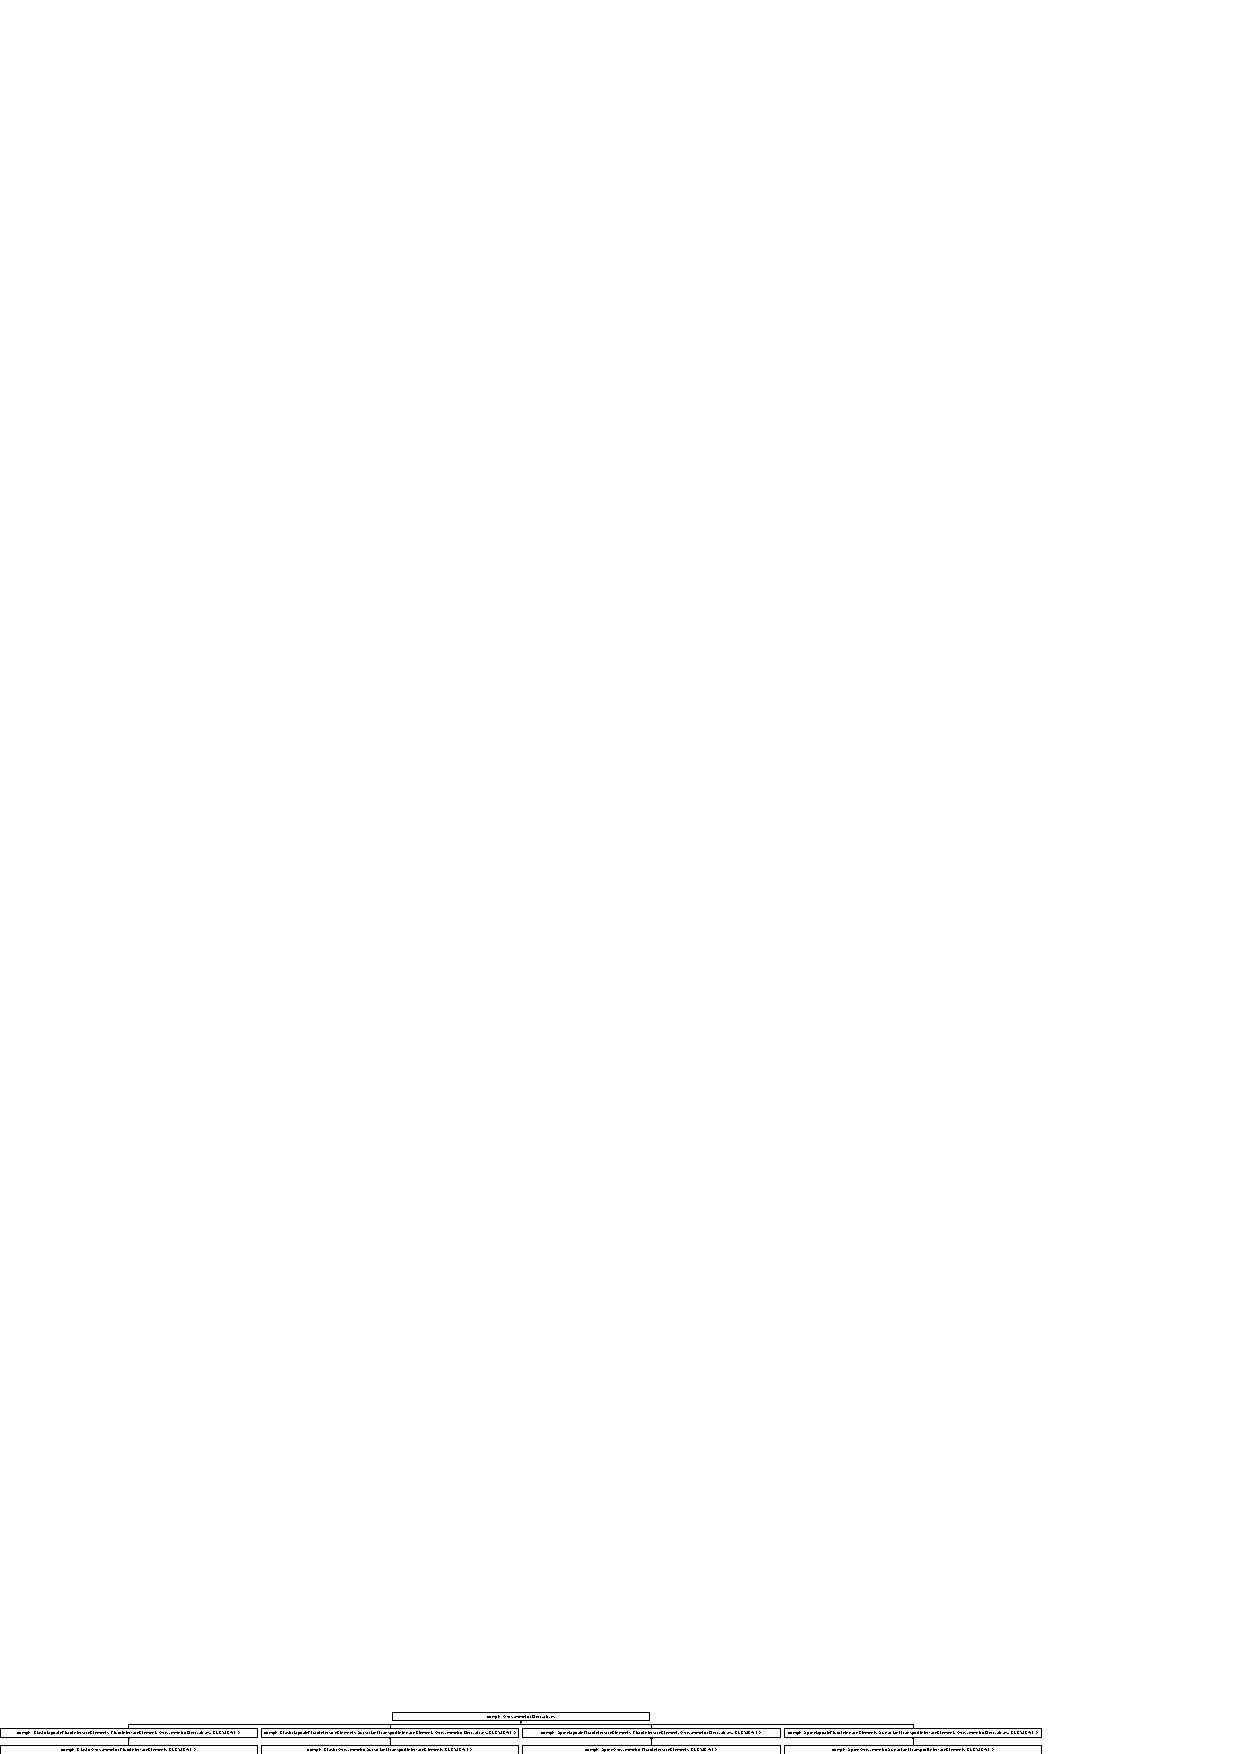
\includegraphics[height=0.794326cm]{classoomph_1_1AxisymmetricDerivatives}
\end{center}
\end{figure}
\subsection*{Public Member Functions}
\begin{DoxyCompactItemize}
\item 
\hyperlink{classoomph_1_1AxisymmetricDerivatives_a91b259ef45c7563b05bf79de4b0fe4bf}{Axisymmetric\+Derivatives} ()
\end{DoxyCompactItemize}
\subsection*{Protected Member Functions}
\begin{DoxyCompactItemize}
\item 
double \hyperlink{classoomph_1_1AxisymmetricDerivatives_a306ea6b57d09d57e87e8d74a13c2f828}{compute\+\_\+surface\+\_\+derivatives} (const Shape \&psi, const D\+Shape \&dpsids, const Dense\+Matrix$<$ double $>$ \&interpolated\+\_\+t, const Vector$<$ double $>$ \&interpolated\+\_\+x, D\+Shape \&surface\+\_\+gradient, D\+Shape \&surface\+\_\+divergence)
\begin{DoxyCompactList}\small\item\em Fill in the specific surface derivative calculations. \end{DoxyCompactList}\end{DoxyCompactItemize}


\subsection{Detailed Description}
Class that establishes the surface derivative functions for Axisymmetric\+Interface\+Elements. These are defined in a separate class so that they can be used by other interface equation-\/type classes. 

Definition at line 669 of file interface\+\_\+elements.\+h.



\subsection{Constructor \& Destructor Documentation}
\mbox{\Hypertarget{classoomph_1_1AxisymmetricDerivatives_a91b259ef45c7563b05bf79de4b0fe4bf}\label{classoomph_1_1AxisymmetricDerivatives_a91b259ef45c7563b05bf79de4b0fe4bf}} 
\index{oomph\+::\+Axisymmetric\+Derivatives@{oomph\+::\+Axisymmetric\+Derivatives}!Axisymmetric\+Derivatives@{Axisymmetric\+Derivatives}}
\index{Axisymmetric\+Derivatives@{Axisymmetric\+Derivatives}!oomph\+::\+Axisymmetric\+Derivatives@{oomph\+::\+Axisymmetric\+Derivatives}}
\subsubsection{\texorpdfstring{Axisymmetric\+Derivatives()}{AxisymmetricDerivatives()}}
{\footnotesize\ttfamily oomph\+::\+Axisymmetric\+Derivatives\+::\+Axisymmetric\+Derivatives (\begin{DoxyParamCaption}{ }\end{DoxyParamCaption})\hspace{0.3cm}{\ttfamily [inline]}}



Definition at line 673 of file interface\+\_\+elements.\+h.



\subsection{Member Function Documentation}
\mbox{\Hypertarget{classoomph_1_1AxisymmetricDerivatives_a306ea6b57d09d57e87e8d74a13c2f828}\label{classoomph_1_1AxisymmetricDerivatives_a306ea6b57d09d57e87e8d74a13c2f828}} 
\index{oomph\+::\+Axisymmetric\+Derivatives@{oomph\+::\+Axisymmetric\+Derivatives}!compute\+\_\+surface\+\_\+derivatives@{compute\+\_\+surface\+\_\+derivatives}}
\index{compute\+\_\+surface\+\_\+derivatives@{compute\+\_\+surface\+\_\+derivatives}!oomph\+::\+Axisymmetric\+Derivatives@{oomph\+::\+Axisymmetric\+Derivatives}}
\subsubsection{\texorpdfstring{compute\+\_\+surface\+\_\+derivatives()}{compute\_surface\_derivatives()}}
{\footnotesize\ttfamily double oomph\+::\+Axisymmetric\+Derivatives\+::compute\+\_\+surface\+\_\+derivatives (\begin{DoxyParamCaption}\item[{const Shape \&}]{psi,  }\item[{const D\+Shape \&}]{dpsids,  }\item[{const Dense\+Matrix$<$ double $>$ \&}]{interpolated\+\_\+t,  }\item[{const Vector$<$ double $>$ \&}]{interpolated\+\_\+x,  }\item[{D\+Shape \&}]{surface\+\_\+gradient,  }\item[{D\+Shape \&}]{surface\+\_\+divergence }\end{DoxyParamCaption})\hspace{0.3cm}{\ttfamily [protected]}}



Fill in the specific surface derivative calculations. 

Specialise the surface derivatives for the axisymmetric interface case. 

Definition at line 803 of file interface\+\_\+elements.\+cc.



The documentation for this class was generated from the following files\+:\begin{DoxyCompactItemize}
\item 
\hyperlink{interface__elements_8h}{interface\+\_\+elements.\+h}\item 
\hyperlink{interface__elements_8cc}{interface\+\_\+elements.\+cc}\end{DoxyCompactItemize}

\hypertarget{classoomph_1_1AxisymmetricVolumeConstraintBoundingElement}{}\section{oomph\+:\+:Axisymmetric\+Volume\+Constraint\+Bounding\+Element Class Reference}
\label{classoomph_1_1AxisymmetricVolumeConstraintBoundingElement}\index{oomph\+::\+Axisymmetric\+Volume\+Constraint\+Bounding\+Element@{oomph\+::\+Axisymmetric\+Volume\+Constraint\+Bounding\+Element}}


{\ttfamily \#include $<$constrained\+\_\+volume\+\_\+elements.\+h$>$}

Inheritance diagram for oomph\+:\+:Axisymmetric\+Volume\+Constraint\+Bounding\+Element\+:\begin{figure}[H]
\begin{center}
\leavevmode
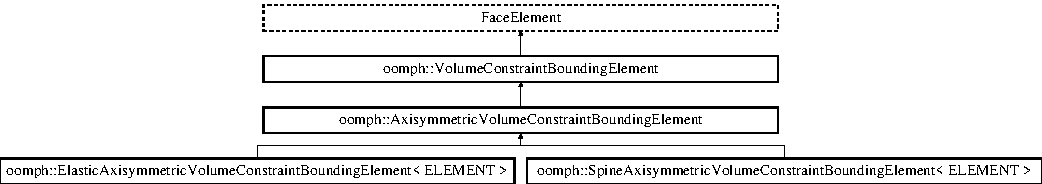
\includegraphics[height=3.716814cm]{classoomph_1_1AxisymmetricVolumeConstraintBoundingElement}
\end{center}
\end{figure}
\subsection*{Public Member Functions}
\begin{DoxyCompactItemize}
\item 
\hyperlink{classoomph_1_1AxisymmetricVolumeConstraintBoundingElement_a716ae91b7c11f6d71c474bec6f6d6d24}{Axisymmetric\+Volume\+Constraint\+Bounding\+Element} ()
\begin{DoxyCompactList}\small\item\em Empty Contructor. \end{DoxyCompactList}\item 
\hyperlink{classoomph_1_1AxisymmetricVolumeConstraintBoundingElement_ac7b98a2915cef69c7e4825e1f5730bc5}{$\sim$\+Axisymmetric\+Volume\+Constraint\+Bounding\+Element} ()
\begin{DoxyCompactList}\small\item\em Empty Destructor. \end{DoxyCompactList}\item 
double \hyperlink{classoomph_1_1AxisymmetricVolumeConstraintBoundingElement_a2d54cd3bce11538b066c8626b241d2c9}{contribution\+\_\+to\+\_\+enclosed\+\_\+volume} ()
\begin{DoxyCompactList}\small\item\em Return this element\textquotesingle{}s contribution to the total volume enclosed. \end{DoxyCompactList}\item 
double \hyperlink{classoomph_1_1AxisymmetricVolumeConstraintBoundingElement_a746f88f325d61610e10e97465fd2ca09}{contribution\+\_\+to\+\_\+volume\+\_\+flux} ()
\begin{DoxyCompactList}\small\item\em Return this element\textquotesingle{}s contribution to the volume flux over the boundary. \end{DoxyCompactList}\end{DoxyCompactItemize}
\subsection*{Protected Member Functions}
\begin{DoxyCompactItemize}
\item 
void \hyperlink{classoomph_1_1AxisymmetricVolumeConstraintBoundingElement_a2a3f3b86079f27d52679f357f5276d91}{fill\+\_\+in\+\_\+generic\+\_\+residual\+\_\+contribution\+\_\+volume\+\_\+constraint} (\hyperlink{classoomph_1_1Vector}{Vector}$<$ double $>$ \&residuals)
\begin{DoxyCompactList}\small\item\em Helper function to fill in contributions to residuals (remember that part of the residual is added by the the associated \hyperlink{classoomph_1_1VolumeConstraintElement}{Volume\+Constraint\+Element}). This is specific for 1D line elements that bound 2D cartesian fluid elements. \end{DoxyCompactList}\end{DoxyCompactItemize}
\subsection*{Additional Inherited Members}


\subsection{Detailed Description}
Axisymmetric (one-\/dimensional) interface elements that allow the application of a volume constraint on the region bounded by these elements. The volume is computed by integrating x.\+n around the boundary of the domain and then dividing by three. The sign is chosen so that the volume will be positive when the elements surround a fluid domain.

These elements must be used together with the associated \hyperlink{classoomph_1_1VolumeConstraintElement}{Volume\+Constraint\+Element}, which stores the value of the target volume. 

Definition at line 493 of file constrained\+\_\+volume\+\_\+elements.\+h.



\subsection{Constructor \& Destructor Documentation}
\mbox{\Hypertarget{classoomph_1_1AxisymmetricVolumeConstraintBoundingElement_a716ae91b7c11f6d71c474bec6f6d6d24}\label{classoomph_1_1AxisymmetricVolumeConstraintBoundingElement_a716ae91b7c11f6d71c474bec6f6d6d24}} 
\index{oomph\+::\+Axisymmetric\+Volume\+Constraint\+Bounding\+Element@{oomph\+::\+Axisymmetric\+Volume\+Constraint\+Bounding\+Element}!Axisymmetric\+Volume\+Constraint\+Bounding\+Element@{Axisymmetric\+Volume\+Constraint\+Bounding\+Element}}
\index{Axisymmetric\+Volume\+Constraint\+Bounding\+Element@{Axisymmetric\+Volume\+Constraint\+Bounding\+Element}!oomph\+::\+Axisymmetric\+Volume\+Constraint\+Bounding\+Element@{oomph\+::\+Axisymmetric\+Volume\+Constraint\+Bounding\+Element}}
\subsubsection{\texorpdfstring{Axisymmetric\+Volume\+Constraint\+Bounding\+Element()}{AxisymmetricVolumeConstraintBoundingElement()}}
{\footnotesize\ttfamily oomph\+::\+Axisymmetric\+Volume\+Constraint\+Bounding\+Element\+::\+Axisymmetric\+Volume\+Constraint\+Bounding\+Element (\begin{DoxyParamCaption}{ }\end{DoxyParamCaption})\hspace{0.3cm}{\ttfamily [inline]}}



Empty Contructor. 



Definition at line 508 of file constrained\+\_\+volume\+\_\+elements.\+h.

\mbox{\Hypertarget{classoomph_1_1AxisymmetricVolumeConstraintBoundingElement_ac7b98a2915cef69c7e4825e1f5730bc5}\label{classoomph_1_1AxisymmetricVolumeConstraintBoundingElement_ac7b98a2915cef69c7e4825e1f5730bc5}} 
\index{oomph\+::\+Axisymmetric\+Volume\+Constraint\+Bounding\+Element@{oomph\+::\+Axisymmetric\+Volume\+Constraint\+Bounding\+Element}!````~Axisymmetric\+Volume\+Constraint\+Bounding\+Element@{$\sim$\+Axisymmetric\+Volume\+Constraint\+Bounding\+Element}}
\index{````~Axisymmetric\+Volume\+Constraint\+Bounding\+Element@{$\sim$\+Axisymmetric\+Volume\+Constraint\+Bounding\+Element}!oomph\+::\+Axisymmetric\+Volume\+Constraint\+Bounding\+Element@{oomph\+::\+Axisymmetric\+Volume\+Constraint\+Bounding\+Element}}
\subsubsection{\texorpdfstring{$\sim$\+Axisymmetric\+Volume\+Constraint\+Bounding\+Element()}{~AxisymmetricVolumeConstraintBoundingElement()}}
{\footnotesize\ttfamily oomph\+::\+Axisymmetric\+Volume\+Constraint\+Bounding\+Element\+::$\sim$\+Axisymmetric\+Volume\+Constraint\+Bounding\+Element (\begin{DoxyParamCaption}{ }\end{DoxyParamCaption})\hspace{0.3cm}{\ttfamily [inline]}}



Empty Destructor. 



Definition at line 512 of file constrained\+\_\+volume\+\_\+elements.\+h.



\subsection{Member Function Documentation}
\mbox{\Hypertarget{classoomph_1_1AxisymmetricVolumeConstraintBoundingElement_a2d54cd3bce11538b066c8626b241d2c9}\label{classoomph_1_1AxisymmetricVolumeConstraintBoundingElement_a2d54cd3bce11538b066c8626b241d2c9}} 
\index{oomph\+::\+Axisymmetric\+Volume\+Constraint\+Bounding\+Element@{oomph\+::\+Axisymmetric\+Volume\+Constraint\+Bounding\+Element}!contribution\+\_\+to\+\_\+enclosed\+\_\+volume@{contribution\+\_\+to\+\_\+enclosed\+\_\+volume}}
\index{contribution\+\_\+to\+\_\+enclosed\+\_\+volume@{contribution\+\_\+to\+\_\+enclosed\+\_\+volume}!oomph\+::\+Axisymmetric\+Volume\+Constraint\+Bounding\+Element@{oomph\+::\+Axisymmetric\+Volume\+Constraint\+Bounding\+Element}}
\subsubsection{\texorpdfstring{contribution\+\_\+to\+\_\+enclosed\+\_\+volume()}{contribution\_to\_enclosed\_volume()}}
{\footnotesize\ttfamily double oomph\+::\+Axisymmetric\+Volume\+Constraint\+Bounding\+Element\+::contribution\+\_\+to\+\_\+enclosed\+\_\+volume (\begin{DoxyParamCaption}{ }\end{DoxyParamCaption})}



Return this element\textquotesingle{}s contribution to the total volume enclosed. 



Definition at line 274 of file constrained\+\_\+volume\+\_\+elements.\+cc.



References oomph\+::\+Vector\+Helpers\+::dot(), fill\+\_\+in\+\_\+generic\+\_\+residual\+\_\+contribution\+\_\+volume\+\_\+constraint(), i, s, and oomph\+::\+Quad\+Tree\+Names\+::W.



Referenced by oomph\+::\+Line\+Volume\+Constraint\+Bounding\+Element\+::contribution\+\_\+to\+\_\+enclosed\+\_\+volume().

\mbox{\Hypertarget{classoomph_1_1AxisymmetricVolumeConstraintBoundingElement_a746f88f325d61610e10e97465fd2ca09}\label{classoomph_1_1AxisymmetricVolumeConstraintBoundingElement_a746f88f325d61610e10e97465fd2ca09}} 
\index{oomph\+::\+Axisymmetric\+Volume\+Constraint\+Bounding\+Element@{oomph\+::\+Axisymmetric\+Volume\+Constraint\+Bounding\+Element}!contribution\+\_\+to\+\_\+volume\+\_\+flux@{contribution\+\_\+to\+\_\+volume\+\_\+flux}}
\index{contribution\+\_\+to\+\_\+volume\+\_\+flux@{contribution\+\_\+to\+\_\+volume\+\_\+flux}!oomph\+::\+Axisymmetric\+Volume\+Constraint\+Bounding\+Element@{oomph\+::\+Axisymmetric\+Volume\+Constraint\+Bounding\+Element}}
\subsubsection{\texorpdfstring{contribution\+\_\+to\+\_\+volume\+\_\+flux()}{contribution\_to\_volume\_flux()}}
{\footnotesize\ttfamily double oomph\+::\+Axisymmetric\+Volume\+Constraint\+Bounding\+Element\+::contribution\+\_\+to\+\_\+volume\+\_\+flux (\begin{DoxyParamCaption}{ }\end{DoxyParamCaption})\hspace{0.3cm}{\ttfamily [inline]}}



Return this element\textquotesingle{}s contribution to the volume flux over the boundary. 



Definition at line 519 of file constrained\+\_\+volume\+\_\+elements.\+h.



References oomph\+::\+Vector\+Helpers\+::dot(), i, s, and oomph\+::\+Quad\+Tree\+Names\+::W.

\mbox{\Hypertarget{classoomph_1_1AxisymmetricVolumeConstraintBoundingElement_a2a3f3b86079f27d52679f357f5276d91}\label{classoomph_1_1AxisymmetricVolumeConstraintBoundingElement_a2a3f3b86079f27d52679f357f5276d91}} 
\index{oomph\+::\+Axisymmetric\+Volume\+Constraint\+Bounding\+Element@{oomph\+::\+Axisymmetric\+Volume\+Constraint\+Bounding\+Element}!fill\+\_\+in\+\_\+generic\+\_\+residual\+\_\+contribution\+\_\+volume\+\_\+constraint@{fill\+\_\+in\+\_\+generic\+\_\+residual\+\_\+contribution\+\_\+volume\+\_\+constraint}}
\index{fill\+\_\+in\+\_\+generic\+\_\+residual\+\_\+contribution\+\_\+volume\+\_\+constraint@{fill\+\_\+in\+\_\+generic\+\_\+residual\+\_\+contribution\+\_\+volume\+\_\+constraint}!oomph\+::\+Axisymmetric\+Volume\+Constraint\+Bounding\+Element@{oomph\+::\+Axisymmetric\+Volume\+Constraint\+Bounding\+Element}}
\subsubsection{\texorpdfstring{fill\+\_\+in\+\_\+generic\+\_\+residual\+\_\+contribution\+\_\+volume\+\_\+constraint()}{fill\_in\_generic\_residual\_contribution\_volume\_constraint()}}
{\footnotesize\ttfamily void oomph\+::\+Axisymmetric\+Volume\+Constraint\+Bounding\+Element\+::fill\+\_\+in\+\_\+generic\+\_\+residual\+\_\+contribution\+\_\+volume\+\_\+constraint (\begin{DoxyParamCaption}\item[{\hyperlink{classoomph_1_1Vector}{Vector}$<$ double $>$ \&}]{residuals }\end{DoxyParamCaption})\hspace{0.3cm}{\ttfamily [protected]}, {\ttfamily [virtual]}}



Helper function to fill in contributions to residuals (remember that part of the residual is added by the the associated \hyperlink{classoomph_1_1VolumeConstraintElement}{Volume\+Constraint\+Element}). This is specific for 1D line elements that bound 2D cartesian fluid elements. 

Helper function to fill in contributions to residuals (remember that part of the residual is added by the the associated \hyperlink{classoomph_1_1VolumeConstraintElement}{Volume\+Constraint\+Element}). This is specific for axisymmetric line elements that bound 2D axisymmetric fluid elements. The only difference from the 1D case is the addition of the weighting factor in the integrand and division of the dot product by three. 

Implements \hyperlink{classoomph_1_1VolumeConstraintBoundingElement_a717f1085709bd8820b8043ff94ecb0c5}{oomph\+::\+Volume\+Constraint\+Bounding\+Element}.



Definition at line 359 of file constrained\+\_\+volume\+\_\+elements.\+cc.



References oomph\+::\+Vector\+Helpers\+::dot(), oomph\+::\+Surface\+Volume\+Constraint\+Bounding\+Element\+::fill\+\_\+in\+\_\+generic\+\_\+residual\+\_\+contribution\+\_\+volume\+\_\+constraint(), i, oomph\+::\+Volume\+Constraint\+Element\+::ptraded\+\_\+local\+\_\+eqn(), s, and oomph\+::\+Quad\+Tree\+Names\+::W.



Referenced by contribution\+\_\+to\+\_\+enclosed\+\_\+volume().



The documentation for this class was generated from the following files\+:\begin{DoxyCompactItemize}
\item 
\hyperlink{constrained__volume__elements_8h}{constrained\+\_\+volume\+\_\+elements.\+h}\item 
\hyperlink{constrained__volume__elements_8cc}{constrained\+\_\+volume\+\_\+elements.\+cc}\end{DoxyCompactItemize}

\hypertarget{classoomph_1_1BoundingElementType}{}\section{oomph\+:\+:Bounding\+Element\+Type$<$ E\+L\+E\+M\+E\+NT $>$ Class Template Reference}
\label{classoomph_1_1BoundingElementType}\index{oomph\+::\+Bounding\+Element\+Type$<$ E\+L\+E\+M\+E\+N\+T $>$@{oomph\+::\+Bounding\+Element\+Type$<$ E\+L\+E\+M\+E\+N\+T $>$}}


This policy class is used to associate specific bounding elements with specific Fluid\+Interface elements. It must be filled in for every class that uses the Spine\+Update\+Fluid\+Interface$<$...$>$ or Elastic\+Update\+Fluid\+Interface$<$....$>$ generic template classes. Examples for our default Line, Axisymmetric and Surface types are included below.  




{\ttfamily \#include $<$specific\+\_\+node\+\_\+update\+\_\+interface\+\_\+elements.\+h$>$}



\subsection{Detailed Description}
\subsubsection*{template$<$class E\+L\+E\+M\+E\+NT$>$\newline
class oomph\+::\+Bounding\+Element\+Type$<$ E\+L\+E\+M\+E\+N\+T $>$}

This policy class is used to associate specific bounding elements with specific Fluid\+Interface elements. It must be filled in for every class that uses the Spine\+Update\+Fluid\+Interface$<$...$>$ or Elastic\+Update\+Fluid\+Interface$<$....$>$ generic template classes. Examples for our default Line, Axisymmetric and Surface types are included below. 

Definition at line 59 of file specific\+\_\+node\+\_\+update\+\_\+interface\+\_\+elements.\+h.



The documentation for this class was generated from the following file\+:\begin{DoxyCompactItemize}
\item 
\hyperlink{specific__node__update__interface__elements_8h}{specific\+\_\+node\+\_\+update\+\_\+interface\+\_\+elements.\+h}\end{DoxyCompactItemize}

\hypertarget{classoomph_1_1BoundingElementType_3_01ElasticUpdateFluidInterfaceElement_3_01FluidInterfaceEleme3184fbb3565ba21902c1c3c09e7b1c72}{}\section{oomph\+:\+:Bounding\+Element\+Type$<$ Elastic\+Update\+Fluid\+Interface\+Element$<$ Fluid\+Interface\+Element, Axisymmetric\+Derivatives, E\+L\+E\+M\+E\+NT $>$ $>$ Class Template Reference}
\label{classoomph_1_1BoundingElementType_3_01ElasticUpdateFluidInterfaceElement_3_01FluidInterfaceEleme3184fbb3565ba21902c1c3c09e7b1c72}\index{oomph\+::\+Bounding\+Element\+Type$<$ Elastic\+Update\+Fluid\+Interface\+Element$<$ Fluid\+Interface\+Element, Axisymmetric\+Derivatives, E\+L\+E\+M\+E\+N\+T $>$ $>$@{oomph\+::\+Bounding\+Element\+Type$<$ Elastic\+Update\+Fluid\+Interface\+Element$<$ Fluid\+Interface\+Element, Axisymmetric\+Derivatives, E\+L\+E\+M\+E\+N\+T $>$ $>$}}


{\ttfamily \#include $<$specific\+\_\+node\+\_\+update\+\_\+interface\+\_\+elements.\+h$>$}

Inheritance diagram for oomph\+:\+:Bounding\+Element\+Type$<$ Elastic\+Update\+Fluid\+Interface\+Element$<$ Fluid\+Interface\+Element, Axisymmetric\+Derivatives, E\+L\+E\+M\+E\+NT $>$ $>$\+:\begin{figure}[H]
\begin{center}
\leavevmode
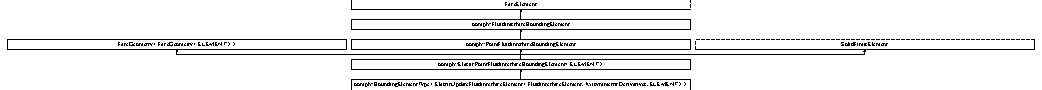
\includegraphics[height=1.212121cm]{classoomph_1_1BoundingElementType_3_01ElasticUpdateFluidInterfaceElement_3_01FluidInterfaceEleme3184fbb3565ba21902c1c3c09e7b1c72}
\end{center}
\end{figure}
\subsection*{Public Member Functions}
\begin{DoxyCompactItemize}
\item 
\hyperlink{classoomph_1_1BoundingElementType_3_01ElasticUpdateFluidInterfaceElement_3_01FluidInterfaceEleme3184fbb3565ba21902c1c3c09e7b1c72_af8a39d59170abd06b1504fcc1c4d84e8}{Bounding\+Element\+Type} ()
\end{DoxyCompactItemize}
\subsection*{Additional Inherited Members}


\subsection{Detailed Description}
\subsubsection*{template$<$class E\+L\+E\+M\+E\+NT$>$\newline
class oomph\+::\+Bounding\+Element\+Type$<$ Elastic\+Update\+Fluid\+Interface\+Element$<$ Fluid\+Interface\+Element, Axisymmetric\+Derivatives, E\+L\+E\+M\+E\+N\+T $>$ $>$}



Definition at line 1111 of file specific\+\_\+node\+\_\+update\+\_\+interface\+\_\+elements.\+h.



\subsection{Constructor \& Destructor Documentation}
\mbox{\Hypertarget{classoomph_1_1BoundingElementType_3_01ElasticUpdateFluidInterfaceElement_3_01FluidInterfaceEleme3184fbb3565ba21902c1c3c09e7b1c72_af8a39d59170abd06b1504fcc1c4d84e8}\label{classoomph_1_1BoundingElementType_3_01ElasticUpdateFluidInterfaceElement_3_01FluidInterfaceEleme3184fbb3565ba21902c1c3c09e7b1c72_af8a39d59170abd06b1504fcc1c4d84e8}} 
\index{oomph\+::\+Bounding\+Element\+Type$<$ Elastic\+Update\+Fluid\+Interface\+Element$<$ Fluid\+Interface\+Element, Axisymmetric\+Derivatives, E\+L\+E\+M\+E\+N\+T $>$ $>$@{oomph\+::\+Bounding\+Element\+Type$<$ Elastic\+Update\+Fluid\+Interface\+Element$<$ Fluid\+Interface\+Element, Axisymmetric\+Derivatives, E\+L\+E\+M\+E\+N\+T $>$ $>$}!Bounding\+Element\+Type@{Bounding\+Element\+Type}}
\index{Bounding\+Element\+Type@{Bounding\+Element\+Type}!oomph\+::\+Bounding\+Element\+Type$<$ Elastic\+Update\+Fluid\+Interface\+Element$<$ Fluid\+Interface\+Element, Axisymmetric\+Derivatives, E\+L\+E\+M\+E\+N\+T $>$ $>$@{oomph\+::\+Bounding\+Element\+Type$<$ Elastic\+Update\+Fluid\+Interface\+Element$<$ Fluid\+Interface\+Element, Axisymmetric\+Derivatives, E\+L\+E\+M\+E\+N\+T $>$ $>$}}
\subsubsection{\texorpdfstring{Bounding\+Element\+Type()}{BoundingElementType()}}
{\footnotesize\ttfamily template$<$class E\+L\+E\+M\+E\+NT $>$ \\
\hyperlink{classoomph_1_1BoundingElementType}{oomph\+::\+Bounding\+Element\+Type}$<$ \hyperlink{classoomph_1_1ElasticUpdateFluidInterfaceElement}{Elastic\+Update\+Fluid\+Interface\+Element}$<$ \hyperlink{classoomph_1_1FluidInterfaceElement}{Fluid\+Interface\+Element}, \hyperlink{classoomph_1_1AxisymmetricDerivatives}{Axisymmetric\+Derivatives}, E\+L\+E\+M\+E\+NT $>$ $>$\+::\hyperlink{classoomph_1_1BoundingElementType}{Bounding\+Element\+Type} (\begin{DoxyParamCaption}{ }\end{DoxyParamCaption})\hspace{0.3cm}{\ttfamily [inline]}}



Definition at line 1118 of file specific\+\_\+node\+\_\+update\+\_\+interface\+\_\+elements.\+h.



The documentation for this class was generated from the following file\+:\begin{DoxyCompactItemize}
\item 
\hyperlink{specific__node__update__interface__elements_8h}{specific\+\_\+node\+\_\+update\+\_\+interface\+\_\+elements.\+h}\end{DoxyCompactItemize}

\hypertarget{classoomph_1_1BoundingElementType_3_01ElasticUpdateFluidInterfaceElement_3_01FluidInterfaceEleme25258208c656cd18bb5e78a946d0c1ca}{}\section{oomph\+:\+:Bounding\+Element\+Type$<$ Elastic\+Update\+Fluid\+Interface\+Element$<$ Fluid\+Interface\+Element, Line\+Derivatives, E\+L\+E\+M\+E\+NT $>$ $>$ Class Template Reference}
\label{classoomph_1_1BoundingElementType_3_01ElasticUpdateFluidInterfaceElement_3_01FluidInterfaceEleme25258208c656cd18bb5e78a946d0c1ca}\index{oomph\+::\+Bounding\+Element\+Type$<$ Elastic\+Update\+Fluid\+Interface\+Element$<$ Fluid\+Interface\+Element, Line\+Derivatives, E\+L\+E\+M\+E\+N\+T $>$ $>$@{oomph\+::\+Bounding\+Element\+Type$<$ Elastic\+Update\+Fluid\+Interface\+Element$<$ Fluid\+Interface\+Element, Line\+Derivatives, E\+L\+E\+M\+E\+N\+T $>$ $>$}}


Define the Bounding\+Element type associated with the 1D surface element.  




{\ttfamily \#include $<$specific\+\_\+node\+\_\+update\+\_\+interface\+\_\+elements.\+h$>$}

Inheritance diagram for oomph\+:\+:Bounding\+Element\+Type$<$ Elastic\+Update\+Fluid\+Interface\+Element$<$ Fluid\+Interface\+Element, Line\+Derivatives, E\+L\+E\+M\+E\+NT $>$ $>$\+:\begin{figure}[H]
\begin{center}
\leavevmode
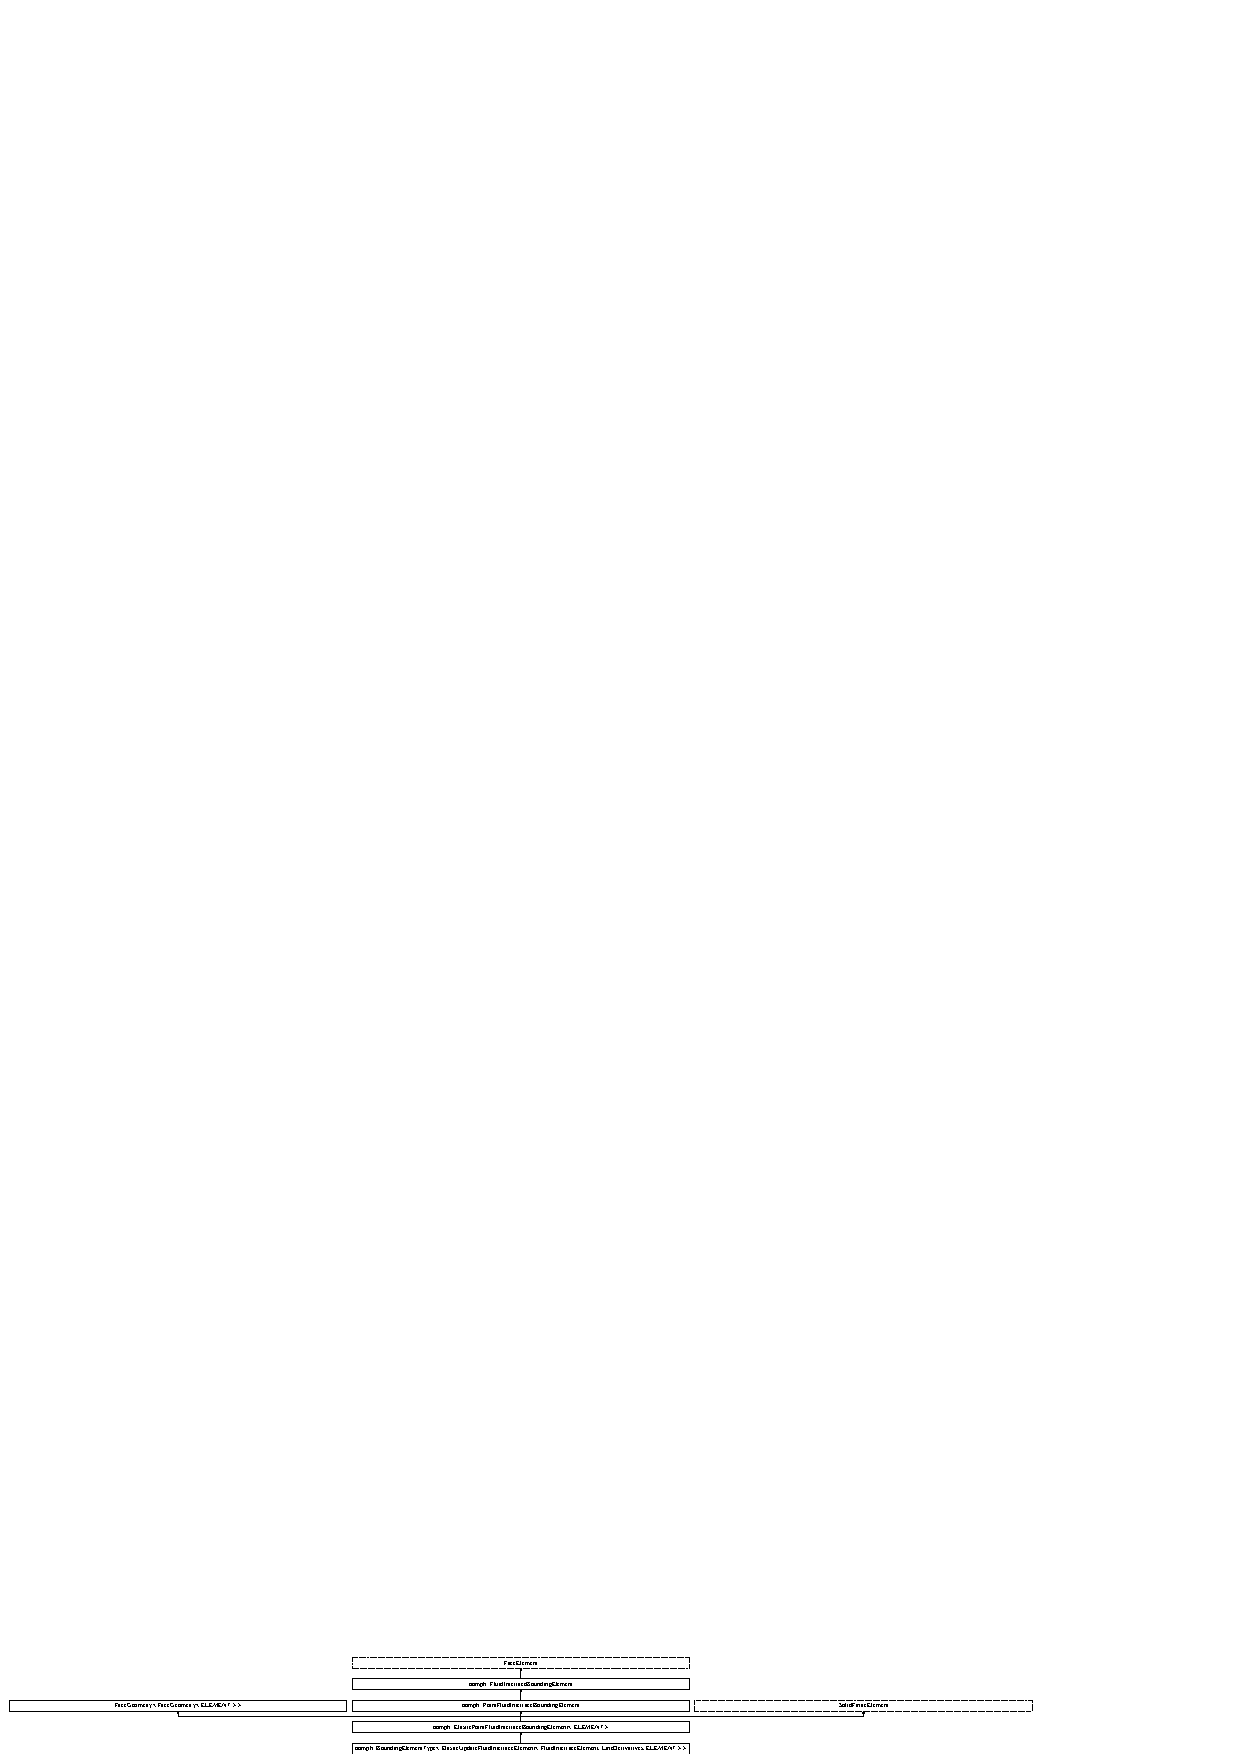
\includegraphics[height=1.361111cm]{classoomph_1_1BoundingElementType_3_01ElasticUpdateFluidInterfaceElement_3_01FluidInterfaceEleme25258208c656cd18bb5e78a946d0c1ca}
\end{center}
\end{figure}
\subsection*{Public Member Functions}
\begin{DoxyCompactItemize}
\item 
\hyperlink{classoomph_1_1BoundingElementType_3_01ElasticUpdateFluidInterfaceElement_3_01FluidInterfaceEleme25258208c656cd18bb5e78a946d0c1ca_a3b2358d710986e238d7e4e5291bc0d1b}{Bounding\+Element\+Type} ()
\end{DoxyCompactItemize}
\subsection*{Additional Inherited Members}


\subsection{Detailed Description}
\subsubsection*{template$<$class E\+L\+E\+M\+E\+NT$>$\newline
class oomph\+::\+Bounding\+Element\+Type$<$ Elastic\+Update\+Fluid\+Interface\+Element$<$ Fluid\+Interface\+Element, Line\+Derivatives, E\+L\+E\+M\+E\+N\+T $>$ $>$}

Define the Bounding\+Element type associated with the 1D surface element. 

Definition at line 1081 of file specific\+\_\+node\+\_\+update\+\_\+interface\+\_\+elements.\+h.



\subsection{Constructor \& Destructor Documentation}
\mbox{\Hypertarget{classoomph_1_1BoundingElementType_3_01ElasticUpdateFluidInterfaceElement_3_01FluidInterfaceEleme25258208c656cd18bb5e78a946d0c1ca_a3b2358d710986e238d7e4e5291bc0d1b}\label{classoomph_1_1BoundingElementType_3_01ElasticUpdateFluidInterfaceElement_3_01FluidInterfaceEleme25258208c656cd18bb5e78a946d0c1ca_a3b2358d710986e238d7e4e5291bc0d1b}} 
\index{oomph\+::\+Bounding\+Element\+Type$<$ Elastic\+Update\+Fluid\+Interface\+Element$<$ Fluid\+Interface\+Element, Line\+Derivatives, E\+L\+E\+M\+E\+N\+T $>$ $>$@{oomph\+::\+Bounding\+Element\+Type$<$ Elastic\+Update\+Fluid\+Interface\+Element$<$ Fluid\+Interface\+Element, Line\+Derivatives, E\+L\+E\+M\+E\+N\+T $>$ $>$}!Bounding\+Element\+Type@{Bounding\+Element\+Type}}
\index{Bounding\+Element\+Type@{Bounding\+Element\+Type}!oomph\+::\+Bounding\+Element\+Type$<$ Elastic\+Update\+Fluid\+Interface\+Element$<$ Fluid\+Interface\+Element, Line\+Derivatives, E\+L\+E\+M\+E\+N\+T $>$ $>$@{oomph\+::\+Bounding\+Element\+Type$<$ Elastic\+Update\+Fluid\+Interface\+Element$<$ Fluid\+Interface\+Element, Line\+Derivatives, E\+L\+E\+M\+E\+N\+T $>$ $>$}}
\subsubsection{\texorpdfstring{Bounding\+Element\+Type()}{BoundingElementType()}}
{\footnotesize\ttfamily template$<$class E\+L\+E\+M\+E\+NT $>$ \\
\hyperlink{classoomph_1_1BoundingElementType}{oomph\+::\+Bounding\+Element\+Type}$<$ \hyperlink{classoomph_1_1ElasticUpdateFluidInterfaceElement}{Elastic\+Update\+Fluid\+Interface\+Element}$<$ \hyperlink{classoomph_1_1FluidInterfaceElement}{Fluid\+Interface\+Element}, \hyperlink{classoomph_1_1LineDerivatives}{Line\+Derivatives}, E\+L\+E\+M\+E\+NT $>$ $>$\+::\hyperlink{classoomph_1_1BoundingElementType}{Bounding\+Element\+Type} (\begin{DoxyParamCaption}{ }\end{DoxyParamCaption})\hspace{0.3cm}{\ttfamily [inline]}}



Definition at line 1088 of file specific\+\_\+node\+\_\+update\+\_\+interface\+\_\+elements.\+h.



The documentation for this class was generated from the following file\+:\begin{DoxyCompactItemize}
\item 
\hyperlink{specific__node__update__interface__elements_8h}{specific\+\_\+node\+\_\+update\+\_\+interface\+\_\+elements.\+h}\end{DoxyCompactItemize}

\hypertarget{classoomph_1_1BoundingElementType_3_01ElasticUpdateFluidInterfaceElement_3_01FluidInterfaceEleme0e022f57b173f7bea5703185db24e722}{}\section{oomph\+:\+:Bounding\+Element\+Type$<$ Elastic\+Update\+Fluid\+Interface\+Element$<$ Fluid\+Interface\+Element, Surface\+Derivatives, E\+L\+E\+M\+E\+NT $>$ $>$ Class Template Reference}
\label{classoomph_1_1BoundingElementType_3_01ElasticUpdateFluidInterfaceElement_3_01FluidInterfaceEleme0e022f57b173f7bea5703185db24e722}\index{oomph\+::\+Bounding\+Element\+Type$<$ Elastic\+Update\+Fluid\+Interface\+Element$<$ Fluid\+Interface\+Element, Surface\+Derivatives, E\+L\+E\+M\+E\+N\+T $>$ $>$@{oomph\+::\+Bounding\+Element\+Type$<$ Elastic\+Update\+Fluid\+Interface\+Element$<$ Fluid\+Interface\+Element, Surface\+Derivatives, E\+L\+E\+M\+E\+N\+T $>$ $>$}}


{\ttfamily \#include $<$specific\+\_\+node\+\_\+update\+\_\+interface\+\_\+elements.\+h$>$}

Inheritance diagram for oomph\+:\+:Bounding\+Element\+Type$<$ Elastic\+Update\+Fluid\+Interface\+Element$<$ Fluid\+Interface\+Element, Surface\+Derivatives, E\+L\+E\+M\+E\+NT $>$ $>$\+:\begin{figure}[H]
\begin{center}
\leavevmode
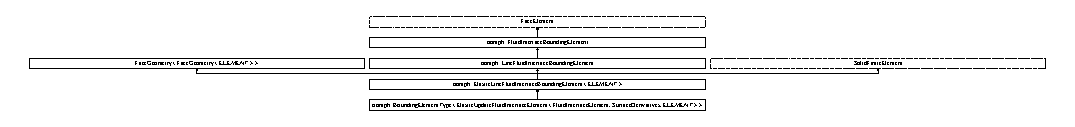
\includegraphics[height=1.322537cm]{classoomph_1_1BoundingElementType_3_01ElasticUpdateFluidInterfaceElement_3_01FluidInterfaceEleme0e022f57b173f7bea5703185db24e722}
\end{center}
\end{figure}
\subsection*{Public Member Functions}
\begin{DoxyCompactItemize}
\item 
\hyperlink{classoomph_1_1BoundingElementType_3_01ElasticUpdateFluidInterfaceElement_3_01FluidInterfaceEleme0e022f57b173f7bea5703185db24e722_a9fbbfa74ad44bc10345170222218ecf1}{Bounding\+Element\+Type} ()
\end{DoxyCompactItemize}
\subsection*{Additional Inherited Members}


\subsection{Detailed Description}
\subsubsection*{template$<$class E\+L\+E\+M\+E\+NT$>$\newline
class oomph\+::\+Bounding\+Element\+Type$<$ Elastic\+Update\+Fluid\+Interface\+Element$<$ Fluid\+Interface\+Element, Surface\+Derivatives, E\+L\+E\+M\+E\+N\+T $>$ $>$}



Definition at line 1141 of file specific\+\_\+node\+\_\+update\+\_\+interface\+\_\+elements.\+h.



\subsection{Constructor \& Destructor Documentation}
\mbox{\Hypertarget{classoomph_1_1BoundingElementType_3_01ElasticUpdateFluidInterfaceElement_3_01FluidInterfaceEleme0e022f57b173f7bea5703185db24e722_a9fbbfa74ad44bc10345170222218ecf1}\label{classoomph_1_1BoundingElementType_3_01ElasticUpdateFluidInterfaceElement_3_01FluidInterfaceEleme0e022f57b173f7bea5703185db24e722_a9fbbfa74ad44bc10345170222218ecf1}} 
\index{oomph\+::\+Bounding\+Element\+Type$<$ Elastic\+Update\+Fluid\+Interface\+Element$<$ Fluid\+Interface\+Element, Surface\+Derivatives, E\+L\+E\+M\+E\+N\+T $>$ $>$@{oomph\+::\+Bounding\+Element\+Type$<$ Elastic\+Update\+Fluid\+Interface\+Element$<$ Fluid\+Interface\+Element, Surface\+Derivatives, E\+L\+E\+M\+E\+N\+T $>$ $>$}!Bounding\+Element\+Type@{Bounding\+Element\+Type}}
\index{Bounding\+Element\+Type@{Bounding\+Element\+Type}!oomph\+::\+Bounding\+Element\+Type$<$ Elastic\+Update\+Fluid\+Interface\+Element$<$ Fluid\+Interface\+Element, Surface\+Derivatives, E\+L\+E\+M\+E\+N\+T $>$ $>$@{oomph\+::\+Bounding\+Element\+Type$<$ Elastic\+Update\+Fluid\+Interface\+Element$<$ Fluid\+Interface\+Element, Surface\+Derivatives, E\+L\+E\+M\+E\+N\+T $>$ $>$}}
\subsubsection{\texorpdfstring{Bounding\+Element\+Type()}{BoundingElementType()}}
{\footnotesize\ttfamily template$<$class E\+L\+E\+M\+E\+NT $>$ \\
\hyperlink{classoomph_1_1BoundingElementType}{oomph\+::\+Bounding\+Element\+Type}$<$ \hyperlink{classoomph_1_1ElasticUpdateFluidInterfaceElement}{Elastic\+Update\+Fluid\+Interface\+Element}$<$ \hyperlink{classoomph_1_1FluidInterfaceElement}{Fluid\+Interface\+Element}, \hyperlink{classoomph_1_1SurfaceDerivatives}{Surface\+Derivatives}, E\+L\+E\+M\+E\+NT $>$ $>$\+::\hyperlink{classoomph_1_1BoundingElementType}{Bounding\+Element\+Type} (\begin{DoxyParamCaption}{ }\end{DoxyParamCaption})\hspace{0.3cm}{\ttfamily [inline]}}



Definition at line 1148 of file specific\+\_\+node\+\_\+update\+\_\+interface\+\_\+elements.\+h.



The documentation for this class was generated from the following file\+:\begin{DoxyCompactItemize}
\item 
\hyperlink{specific__node__update__interface__elements_8h}{specific\+\_\+node\+\_\+update\+\_\+interface\+\_\+elements.\+h}\end{DoxyCompactItemize}

\hypertarget{classoomph_1_1BoundingElementType_3_01ElasticUpdateFluidInterfaceElement_3_01SurfactantTransportdc53e7a70087d96a28c80f422fe03679}{}\section{oomph\+:\+:Bounding\+Element\+Type$<$ Elastic\+Update\+Fluid\+Interface\+Element$<$ Surfactant\+Transport\+Interface\+Element, Axisymmetric\+Derivatives, E\+L\+E\+M\+E\+NT $>$ $>$ Class Template Reference}
\label{classoomph_1_1BoundingElementType_3_01ElasticUpdateFluidInterfaceElement_3_01SurfactantTransportdc53e7a70087d96a28c80f422fe03679}\index{oomph\+::\+Bounding\+Element\+Type$<$ Elastic\+Update\+Fluid\+Interface\+Element$<$ Surfactant\+Transport\+Interface\+Element, Axisymmetric\+Derivatives, E\+L\+E\+M\+E\+N\+T $>$ $>$@{oomph\+::\+Bounding\+Element\+Type$<$ Elastic\+Update\+Fluid\+Interface\+Element$<$ Surfactant\+Transport\+Interface\+Element, Axisymmetric\+Derivatives, E\+L\+E\+M\+E\+N\+T $>$ $>$}}


{\ttfamily \#include $<$surfactant\+\_\+transport\+\_\+elements.\+h$>$}

Inheritance diagram for oomph\+:\+:Bounding\+Element\+Type$<$ Elastic\+Update\+Fluid\+Interface\+Element$<$ Surfactant\+Transport\+Interface\+Element, Axisymmetric\+Derivatives, E\+L\+E\+M\+E\+NT $>$ $>$\+:\begin{figure}[H]
\begin{center}
\leavevmode
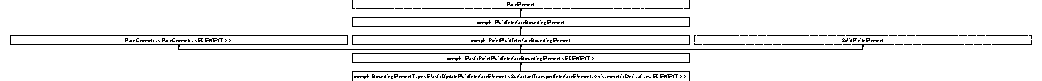
\includegraphics[height=1.092896cm]{classoomph_1_1BoundingElementType_3_01ElasticUpdateFluidInterfaceElement_3_01SurfactantTransportdc53e7a70087d96a28c80f422fe03679}
\end{center}
\end{figure}
\subsection*{Public Member Functions}
\begin{DoxyCompactItemize}
\item 
\hyperlink{classoomph_1_1BoundingElementType_3_01ElasticUpdateFluidInterfaceElement_3_01SurfactantTransportdc53e7a70087d96a28c80f422fe03679_a0ab9a7c644e0ea79321d11c5e661099a}{Bounding\+Element\+Type} ()
\end{DoxyCompactItemize}
\subsection*{Additional Inherited Members}


\subsection{Detailed Description}
\subsubsection*{template$<$class E\+L\+E\+M\+E\+NT$>$\newline
class oomph\+::\+Bounding\+Element\+Type$<$ Elastic\+Update\+Fluid\+Interface\+Element$<$ Surfactant\+Transport\+Interface\+Element, Axisymmetric\+Derivatives, E\+L\+E\+M\+E\+N\+T $>$ $>$}



Definition at line 277 of file surfactant\+\_\+transport\+\_\+elements.\+h.



\subsection{Constructor \& Destructor Documentation}
\mbox{\Hypertarget{classoomph_1_1BoundingElementType_3_01ElasticUpdateFluidInterfaceElement_3_01SurfactantTransportdc53e7a70087d96a28c80f422fe03679_a0ab9a7c644e0ea79321d11c5e661099a}\label{classoomph_1_1BoundingElementType_3_01ElasticUpdateFluidInterfaceElement_3_01SurfactantTransportdc53e7a70087d96a28c80f422fe03679_a0ab9a7c644e0ea79321d11c5e661099a}} 
\index{oomph\+::\+Bounding\+Element\+Type$<$ Elastic\+Update\+Fluid\+Interface\+Element$<$ Surfactant\+Transport\+Interface\+Element, Axisymmetric\+Derivatives, E\+L\+E\+M\+E\+N\+T $>$ $>$@{oomph\+::\+Bounding\+Element\+Type$<$ Elastic\+Update\+Fluid\+Interface\+Element$<$ Surfactant\+Transport\+Interface\+Element, Axisymmetric\+Derivatives, E\+L\+E\+M\+E\+N\+T $>$ $>$}!Bounding\+Element\+Type@{Bounding\+Element\+Type}}
\index{Bounding\+Element\+Type@{Bounding\+Element\+Type}!oomph\+::\+Bounding\+Element\+Type$<$ Elastic\+Update\+Fluid\+Interface\+Element$<$ Surfactant\+Transport\+Interface\+Element, Axisymmetric\+Derivatives, E\+L\+E\+M\+E\+N\+T $>$ $>$@{oomph\+::\+Bounding\+Element\+Type$<$ Elastic\+Update\+Fluid\+Interface\+Element$<$ Surfactant\+Transport\+Interface\+Element, Axisymmetric\+Derivatives, E\+L\+E\+M\+E\+N\+T $>$ $>$}}
\subsubsection{\texorpdfstring{Bounding\+Element\+Type()}{BoundingElementType()}}
{\footnotesize\ttfamily template$<$class E\+L\+E\+M\+E\+NT $>$ \\
\hyperlink{classoomph_1_1BoundingElementType}{oomph\+::\+Bounding\+Element\+Type}$<$ \hyperlink{classoomph_1_1ElasticUpdateFluidInterfaceElement}{Elastic\+Update\+Fluid\+Interface\+Element}$<$ \hyperlink{classoomph_1_1SurfactantTransportInterfaceElement}{Surfactant\+Transport\+Interface\+Element}, \hyperlink{classoomph_1_1AxisymmetricDerivatives}{Axisymmetric\+Derivatives}, E\+L\+E\+M\+E\+NT $>$ $>$\+::\hyperlink{classoomph_1_1BoundingElementType}{Bounding\+Element\+Type} (\begin{DoxyParamCaption}{ }\end{DoxyParamCaption})\hspace{0.3cm}{\ttfamily [inline]}}



Definition at line 284 of file surfactant\+\_\+transport\+\_\+elements.\+h.



The documentation for this class was generated from the following file\+:\begin{DoxyCompactItemize}
\item 
\hyperlink{surfactant__transport__elements_8h}{surfactant\+\_\+transport\+\_\+elements.\+h}\end{DoxyCompactItemize}

\hypertarget{classoomph_1_1BoundingElementType_3_01SpineUpdateFluidInterfaceElement_3_01FluidInterfaceElement7e4c3b8d4bf0b8ea24b4420ab41b2522}{}\section{oomph\+:\+:Bounding\+Element\+Type$<$ Spine\+Update\+Fluid\+Interface\+Element$<$ Fluid\+Interface\+Element, Axisymmetric\+Derivatives, E\+L\+E\+M\+E\+NT $>$ $>$ Class Template Reference}
\label{classoomph_1_1BoundingElementType_3_01SpineUpdateFluidInterfaceElement_3_01FluidInterfaceElement7e4c3b8d4bf0b8ea24b4420ab41b2522}\index{oomph\+::\+Bounding\+Element\+Type$<$ Spine\+Update\+Fluid\+Interface\+Element$<$ Fluid\+Interface\+Element, Axisymmetric\+Derivatives, E\+L\+E\+M\+E\+N\+T $>$ $>$@{oomph\+::\+Bounding\+Element\+Type$<$ Spine\+Update\+Fluid\+Interface\+Element$<$ Fluid\+Interface\+Element, Axisymmetric\+Derivatives, E\+L\+E\+M\+E\+N\+T $>$ $>$}}


{\ttfamily \#include $<$specific\+\_\+node\+\_\+update\+\_\+interface\+\_\+elements.\+h$>$}

Inheritance diagram for oomph\+:\+:Bounding\+Element\+Type$<$ Spine\+Update\+Fluid\+Interface\+Element$<$ Fluid\+Interface\+Element, Axisymmetric\+Derivatives, E\+L\+E\+M\+E\+NT $>$ $>$\+:\begin{figure}[H]
\begin{center}
\leavevmode
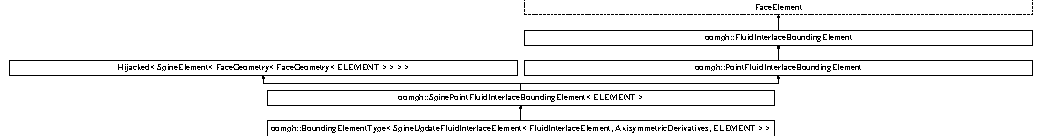
\includegraphics[height=1.830065cm]{classoomph_1_1BoundingElementType_3_01SpineUpdateFluidInterfaceElement_3_01FluidInterfaceElement7e4c3b8d4bf0b8ea24b4420ab41b2522}
\end{center}
\end{figure}
\subsection*{Public Member Functions}
\begin{DoxyCompactItemize}
\item 
\hyperlink{classoomph_1_1BoundingElementType_3_01SpineUpdateFluidInterfaceElement_3_01FluidInterfaceElement7e4c3b8d4bf0b8ea24b4420ab41b2522_a3406b4ef60c81a9019c6c80114e020bf}{Bounding\+Element\+Type} ()
\end{DoxyCompactItemize}
\subsection*{Additional Inherited Members}


\subsection{Detailed Description}
\subsubsection*{template$<$class E\+L\+E\+M\+E\+NT$>$\newline
class oomph\+::\+Bounding\+Element\+Type$<$ Spine\+Update\+Fluid\+Interface\+Element$<$ Fluid\+Interface\+Element, Axisymmetric\+Derivatives, E\+L\+E\+M\+E\+N\+T $>$ $>$}



Definition at line 540 of file specific\+\_\+node\+\_\+update\+\_\+interface\+\_\+elements.\+h.



\subsection{Constructor \& Destructor Documentation}
\mbox{\Hypertarget{classoomph_1_1BoundingElementType_3_01SpineUpdateFluidInterfaceElement_3_01FluidInterfaceElement7e4c3b8d4bf0b8ea24b4420ab41b2522_a3406b4ef60c81a9019c6c80114e020bf}\label{classoomph_1_1BoundingElementType_3_01SpineUpdateFluidInterfaceElement_3_01FluidInterfaceElement7e4c3b8d4bf0b8ea24b4420ab41b2522_a3406b4ef60c81a9019c6c80114e020bf}} 
\index{oomph\+::\+Bounding\+Element\+Type$<$ Spine\+Update\+Fluid\+Interface\+Element$<$ Fluid\+Interface\+Element, Axisymmetric\+Derivatives, E\+L\+E\+M\+E\+N\+T $>$ $>$@{oomph\+::\+Bounding\+Element\+Type$<$ Spine\+Update\+Fluid\+Interface\+Element$<$ Fluid\+Interface\+Element, Axisymmetric\+Derivatives, E\+L\+E\+M\+E\+N\+T $>$ $>$}!Bounding\+Element\+Type@{Bounding\+Element\+Type}}
\index{Bounding\+Element\+Type@{Bounding\+Element\+Type}!oomph\+::\+Bounding\+Element\+Type$<$ Spine\+Update\+Fluid\+Interface\+Element$<$ Fluid\+Interface\+Element, Axisymmetric\+Derivatives, E\+L\+E\+M\+E\+N\+T $>$ $>$@{oomph\+::\+Bounding\+Element\+Type$<$ Spine\+Update\+Fluid\+Interface\+Element$<$ Fluid\+Interface\+Element, Axisymmetric\+Derivatives, E\+L\+E\+M\+E\+N\+T $>$ $>$}}
\subsubsection{\texorpdfstring{Bounding\+Element\+Type()}{BoundingElementType()}}
{\footnotesize\ttfamily template$<$class E\+L\+E\+M\+E\+NT $>$ \\
\hyperlink{classoomph_1_1BoundingElementType}{oomph\+::\+Bounding\+Element\+Type}$<$ \hyperlink{classoomph_1_1SpineUpdateFluidInterfaceElement}{Spine\+Update\+Fluid\+Interface\+Element}$<$ \hyperlink{classoomph_1_1FluidInterfaceElement}{Fluid\+Interface\+Element}, \hyperlink{classoomph_1_1AxisymmetricDerivatives}{Axisymmetric\+Derivatives}, E\+L\+E\+M\+E\+NT $>$ $>$\+::\hyperlink{classoomph_1_1BoundingElementType}{Bounding\+Element\+Type} (\begin{DoxyParamCaption}{ }\end{DoxyParamCaption})\hspace{0.3cm}{\ttfamily [inline]}}



Definition at line 547 of file specific\+\_\+node\+\_\+update\+\_\+interface\+\_\+elements.\+h.



The documentation for this class was generated from the following file\+:\begin{DoxyCompactItemize}
\item 
\hyperlink{specific__node__update__interface__elements_8h}{specific\+\_\+node\+\_\+update\+\_\+interface\+\_\+elements.\+h}\end{DoxyCompactItemize}

\hypertarget{classoomph_1_1BoundingElementType_3_01SpineUpdateFluidInterfaceElement_3_01FluidInterfaceElement0079ff469c68e949ddcf7a17f32ba6a9}{}\section{oomph\+:\+:Bounding\+Element\+Type$<$ Spine\+Update\+Fluid\+Interface\+Element$<$ Fluid\+Interface\+Element, Line\+Derivatives, E\+L\+E\+M\+E\+NT $>$ $>$ Class Template Reference}
\label{classoomph_1_1BoundingElementType_3_01SpineUpdateFluidInterfaceElement_3_01FluidInterfaceElement0079ff469c68e949ddcf7a17f32ba6a9}\index{oomph\+::\+Bounding\+Element\+Type$<$ Spine\+Update\+Fluid\+Interface\+Element$<$ Fluid\+Interface\+Element, Line\+Derivatives, E\+L\+E\+M\+E\+N\+T $>$ $>$@{oomph\+::\+Bounding\+Element\+Type$<$ Spine\+Update\+Fluid\+Interface\+Element$<$ Fluid\+Interface\+Element, Line\+Derivatives, E\+L\+E\+M\+E\+N\+T $>$ $>$}}


{\ttfamily \#include $<$specific\+\_\+node\+\_\+update\+\_\+interface\+\_\+elements.\+h$>$}

Inheritance diagram for oomph\+:\+:Bounding\+Element\+Type$<$ Spine\+Update\+Fluid\+Interface\+Element$<$ Fluid\+Interface\+Element, Line\+Derivatives, E\+L\+E\+M\+E\+NT $>$ $>$\+:\begin{figure}[H]
\begin{center}
\leavevmode
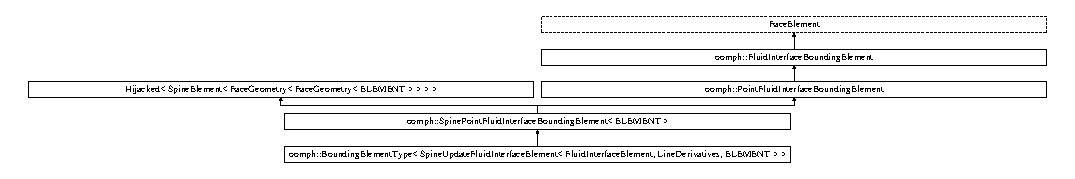
\includegraphics[height=1.253147cm]{classoomph_1_1BoundingElementType_3_01SpineUpdateFluidInterfaceElement_3_01FluidInterfaceElement0079ff469c68e949ddcf7a17f32ba6a9}
\end{center}
\end{figure}
\subsection*{Public Member Functions}
\begin{DoxyCompactItemize}
\item 
\hyperlink{classoomph_1_1BoundingElementType_3_01SpineUpdateFluidInterfaceElement_3_01FluidInterfaceElement0079ff469c68e949ddcf7a17f32ba6a9_ad029328a1fc0ed3b864f41e980601f70}{Bounding\+Element\+Type} ()
\end{DoxyCompactItemize}
\subsection*{Additional Inherited Members}


\subsection{Detailed Description}
\subsubsection*{template$<$class E\+L\+E\+M\+E\+NT$>$\newline
class oomph\+::\+Bounding\+Element\+Type$<$ Spine\+Update\+Fluid\+Interface\+Element$<$ Fluid\+Interface\+Element, Line\+Derivatives, E\+L\+E\+M\+E\+N\+T $>$ $>$}



Definition at line 511 of file specific\+\_\+node\+\_\+update\+\_\+interface\+\_\+elements.\+h.



\subsection{Constructor \& Destructor Documentation}
\mbox{\Hypertarget{classoomph_1_1BoundingElementType_3_01SpineUpdateFluidInterfaceElement_3_01FluidInterfaceElement0079ff469c68e949ddcf7a17f32ba6a9_ad029328a1fc0ed3b864f41e980601f70}\label{classoomph_1_1BoundingElementType_3_01SpineUpdateFluidInterfaceElement_3_01FluidInterfaceElement0079ff469c68e949ddcf7a17f32ba6a9_ad029328a1fc0ed3b864f41e980601f70}} 
\index{oomph\+::\+Bounding\+Element\+Type$<$ Spine\+Update\+Fluid\+Interface\+Element$<$ Fluid\+Interface\+Element, Line\+Derivatives, E\+L\+E\+M\+E\+N\+T $>$ $>$@{oomph\+::\+Bounding\+Element\+Type$<$ Spine\+Update\+Fluid\+Interface\+Element$<$ Fluid\+Interface\+Element, Line\+Derivatives, E\+L\+E\+M\+E\+N\+T $>$ $>$}!Bounding\+Element\+Type@{Bounding\+Element\+Type}}
\index{Bounding\+Element\+Type@{Bounding\+Element\+Type}!oomph\+::\+Bounding\+Element\+Type$<$ Spine\+Update\+Fluid\+Interface\+Element$<$ Fluid\+Interface\+Element, Line\+Derivatives, E\+L\+E\+M\+E\+N\+T $>$ $>$@{oomph\+::\+Bounding\+Element\+Type$<$ Spine\+Update\+Fluid\+Interface\+Element$<$ Fluid\+Interface\+Element, Line\+Derivatives, E\+L\+E\+M\+E\+N\+T $>$ $>$}}
\subsubsection{\texorpdfstring{Bounding\+Element\+Type()}{BoundingElementType()}}
{\footnotesize\ttfamily template$<$class E\+L\+E\+M\+E\+NT $>$ \\
\hyperlink{classoomph_1_1BoundingElementType}{oomph\+::\+Bounding\+Element\+Type}$<$ \hyperlink{classoomph_1_1SpineUpdateFluidInterfaceElement}{Spine\+Update\+Fluid\+Interface\+Element}$<$ \hyperlink{classoomph_1_1FluidInterfaceElement}{Fluid\+Interface\+Element}, \hyperlink{classoomph_1_1LineDerivatives}{Line\+Derivatives}, E\+L\+E\+M\+E\+NT $>$ $>$\+::\hyperlink{classoomph_1_1BoundingElementType}{Bounding\+Element\+Type} (\begin{DoxyParamCaption}{ }\end{DoxyParamCaption})\hspace{0.3cm}{\ttfamily [inline]}}



Definition at line 518 of file specific\+\_\+node\+\_\+update\+\_\+interface\+\_\+elements.\+h.



The documentation for this class was generated from the following file\+:\begin{DoxyCompactItemize}
\item 
\hyperlink{specific__node__update__interface__elements_8h}{specific\+\_\+node\+\_\+update\+\_\+interface\+\_\+elements.\+h}\end{DoxyCompactItemize}

\hypertarget{classoomph_1_1BoundingElementType_3_01SpineUpdateFluidInterfaceElement_3_01FluidInterfaceElement967a9cdd4c55a2ab80dbfbe6be84b5ab}{}\section{oomph\+:\+:Bounding\+Element\+Type$<$ Spine\+Update\+Fluid\+Interface\+Element$<$ Fluid\+Interface\+Element, Surface\+Derivatives, E\+L\+E\+M\+E\+NT $>$ $>$ Class Template Reference}
\label{classoomph_1_1BoundingElementType_3_01SpineUpdateFluidInterfaceElement_3_01FluidInterfaceElement967a9cdd4c55a2ab80dbfbe6be84b5ab}\index{oomph\+::\+Bounding\+Element\+Type$<$ Spine\+Update\+Fluid\+Interface\+Element$<$ Fluid\+Interface\+Element, Surface\+Derivatives, E\+L\+E\+M\+E\+N\+T $>$ $>$@{oomph\+::\+Bounding\+Element\+Type$<$ Spine\+Update\+Fluid\+Interface\+Element$<$ Fluid\+Interface\+Element, Surface\+Derivatives, E\+L\+E\+M\+E\+N\+T $>$ $>$}}


{\ttfamily \#include $<$specific\+\_\+node\+\_\+update\+\_\+interface\+\_\+elements.\+h$>$}

Inheritance diagram for oomph\+:\+:Bounding\+Element\+Type$<$ Spine\+Update\+Fluid\+Interface\+Element$<$ Fluid\+Interface\+Element, Surface\+Derivatives, E\+L\+E\+M\+E\+NT $>$ $>$\+:\begin{figure}[H]
\begin{center}
\leavevmode
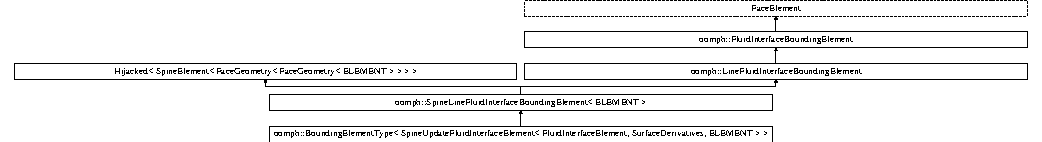
\includegraphics[height=1.217391cm]{classoomph_1_1BoundingElementType_3_01SpineUpdateFluidInterfaceElement_3_01FluidInterfaceElement967a9cdd4c55a2ab80dbfbe6be84b5ab}
\end{center}
\end{figure}
\subsection*{Public Member Functions}
\begin{DoxyCompactItemize}
\item 
\hyperlink{classoomph_1_1BoundingElementType_3_01SpineUpdateFluidInterfaceElement_3_01FluidInterfaceElement967a9cdd4c55a2ab80dbfbe6be84b5ab_a5712fbbcfadc0510cd217141facaa0a2}{Bounding\+Element\+Type} ()
\end{DoxyCompactItemize}
\subsection*{Additional Inherited Members}


\subsection{Detailed Description}
\subsubsection*{template$<$class E\+L\+E\+M\+E\+NT$>$\newline
class oomph\+::\+Bounding\+Element\+Type$<$ Spine\+Update\+Fluid\+Interface\+Element$<$ Fluid\+Interface\+Element, Surface\+Derivatives, E\+L\+E\+M\+E\+N\+T $>$ $>$}



Definition at line 568 of file specific\+\_\+node\+\_\+update\+\_\+interface\+\_\+elements.\+h.



\subsection{Constructor \& Destructor Documentation}
\mbox{\Hypertarget{classoomph_1_1BoundingElementType_3_01SpineUpdateFluidInterfaceElement_3_01FluidInterfaceElement967a9cdd4c55a2ab80dbfbe6be84b5ab_a5712fbbcfadc0510cd217141facaa0a2}\label{classoomph_1_1BoundingElementType_3_01SpineUpdateFluidInterfaceElement_3_01FluidInterfaceElement967a9cdd4c55a2ab80dbfbe6be84b5ab_a5712fbbcfadc0510cd217141facaa0a2}} 
\index{oomph\+::\+Bounding\+Element\+Type$<$ Spine\+Update\+Fluid\+Interface\+Element$<$ Fluid\+Interface\+Element, Surface\+Derivatives, E\+L\+E\+M\+E\+N\+T $>$ $>$@{oomph\+::\+Bounding\+Element\+Type$<$ Spine\+Update\+Fluid\+Interface\+Element$<$ Fluid\+Interface\+Element, Surface\+Derivatives, E\+L\+E\+M\+E\+N\+T $>$ $>$}!Bounding\+Element\+Type@{Bounding\+Element\+Type}}
\index{Bounding\+Element\+Type@{Bounding\+Element\+Type}!oomph\+::\+Bounding\+Element\+Type$<$ Spine\+Update\+Fluid\+Interface\+Element$<$ Fluid\+Interface\+Element, Surface\+Derivatives, E\+L\+E\+M\+E\+N\+T $>$ $>$@{oomph\+::\+Bounding\+Element\+Type$<$ Spine\+Update\+Fluid\+Interface\+Element$<$ Fluid\+Interface\+Element, Surface\+Derivatives, E\+L\+E\+M\+E\+N\+T $>$ $>$}}
\subsubsection{\texorpdfstring{Bounding\+Element\+Type()}{BoundingElementType()}}
{\footnotesize\ttfamily template$<$class E\+L\+E\+M\+E\+NT $>$ \\
\hyperlink{classoomph_1_1BoundingElementType}{oomph\+::\+Bounding\+Element\+Type}$<$ \hyperlink{classoomph_1_1SpineUpdateFluidInterfaceElement}{Spine\+Update\+Fluid\+Interface\+Element}$<$ \hyperlink{classoomph_1_1FluidInterfaceElement}{Fluid\+Interface\+Element}, \hyperlink{classoomph_1_1SurfaceDerivatives}{Surface\+Derivatives}, E\+L\+E\+M\+E\+NT $>$ $>$\+::\hyperlink{classoomph_1_1BoundingElementType}{Bounding\+Element\+Type} (\begin{DoxyParamCaption}{ }\end{DoxyParamCaption})\hspace{0.3cm}{\ttfamily [inline]}}



Definition at line 575 of file specific\+\_\+node\+\_\+update\+\_\+interface\+\_\+elements.\+h.



The documentation for this class was generated from the following file\+:\begin{DoxyCompactItemize}
\item 
\hyperlink{specific__node__update__interface__elements_8h}{specific\+\_\+node\+\_\+update\+\_\+interface\+\_\+elements.\+h}\end{DoxyCompactItemize}

\hypertarget{classoomph_1_1BoundingElementType_3_01SpineUpdateFluidInterfaceElement_3_01SurfactantTransportIn96bc27501b38520de44b2adcd1d39239}{}\section{oomph\+:\+:Bounding\+Element\+Type$<$ Spine\+Update\+Fluid\+Interface\+Element$<$ Surfactant\+Transport\+Interface\+Element, Axisymmetric\+Derivatives, E\+L\+E\+M\+E\+NT $>$ $>$ Class Template Reference}
\label{classoomph_1_1BoundingElementType_3_01SpineUpdateFluidInterfaceElement_3_01SurfactantTransportIn96bc27501b38520de44b2adcd1d39239}\index{oomph\+::\+Bounding\+Element\+Type$<$ Spine\+Update\+Fluid\+Interface\+Element$<$ Surfactant\+Transport\+Interface\+Element, Axisymmetric\+Derivatives, E\+L\+E\+M\+E\+N\+T $>$ $>$@{oomph\+::\+Bounding\+Element\+Type$<$ Spine\+Update\+Fluid\+Interface\+Element$<$ Surfactant\+Transport\+Interface\+Element, Axisymmetric\+Derivatives, E\+L\+E\+M\+E\+N\+T $>$ $>$}}


{\ttfamily \#include $<$surfactant\+\_\+transport\+\_\+elements.\+h$>$}

Inheritance diagram for oomph\+:\+:Bounding\+Element\+Type$<$ Spine\+Update\+Fluid\+Interface\+Element$<$ Surfactant\+Transport\+Interface\+Element, Axisymmetric\+Derivatives, E\+L\+E\+M\+E\+NT $>$ $>$\+:\begin{figure}[H]
\begin{center}
\leavevmode
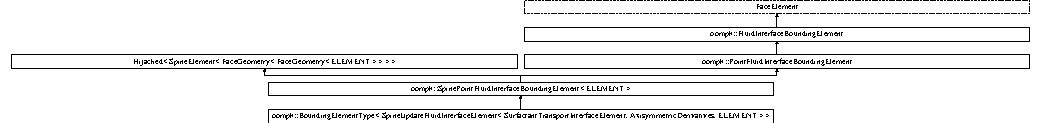
\includegraphics[height=1.055359cm]{classoomph_1_1BoundingElementType_3_01SpineUpdateFluidInterfaceElement_3_01SurfactantTransportIn96bc27501b38520de44b2adcd1d39239}
\end{center}
\end{figure}
\subsection*{Public Member Functions}
\begin{DoxyCompactItemize}
\item 
\hyperlink{classoomph_1_1BoundingElementType_3_01SpineUpdateFluidInterfaceElement_3_01SurfactantTransportIn96bc27501b38520de44b2adcd1d39239_ac2e8a92c0183f1ef76c05e1a20e45ba0}{Bounding\+Element\+Type} ()
\end{DoxyCompactItemize}
\subsection*{Additional Inherited Members}


\subsection{Detailed Description}
\subsubsection*{template$<$class E\+L\+E\+M\+E\+NT$>$\newline
class oomph\+::\+Bounding\+Element\+Type$<$ Spine\+Update\+Fluid\+Interface\+Element$<$ Surfactant\+Transport\+Interface\+Element, Axisymmetric\+Derivatives, E\+L\+E\+M\+E\+N\+T $>$ $>$}



Definition at line 248 of file surfactant\+\_\+transport\+\_\+elements.\+h.



\subsection{Constructor \& Destructor Documentation}
\mbox{\Hypertarget{classoomph_1_1BoundingElementType_3_01SpineUpdateFluidInterfaceElement_3_01SurfactantTransportIn96bc27501b38520de44b2adcd1d39239_ac2e8a92c0183f1ef76c05e1a20e45ba0}\label{classoomph_1_1BoundingElementType_3_01SpineUpdateFluidInterfaceElement_3_01SurfactantTransportIn96bc27501b38520de44b2adcd1d39239_ac2e8a92c0183f1ef76c05e1a20e45ba0}} 
\index{oomph\+::\+Bounding\+Element\+Type$<$ Spine\+Update\+Fluid\+Interface\+Element$<$ Surfactant\+Transport\+Interface\+Element, Axisymmetric\+Derivatives, E\+L\+E\+M\+E\+N\+T $>$ $>$@{oomph\+::\+Bounding\+Element\+Type$<$ Spine\+Update\+Fluid\+Interface\+Element$<$ Surfactant\+Transport\+Interface\+Element, Axisymmetric\+Derivatives, E\+L\+E\+M\+E\+N\+T $>$ $>$}!Bounding\+Element\+Type@{Bounding\+Element\+Type}}
\index{Bounding\+Element\+Type@{Bounding\+Element\+Type}!oomph\+::\+Bounding\+Element\+Type$<$ Spine\+Update\+Fluid\+Interface\+Element$<$ Surfactant\+Transport\+Interface\+Element, Axisymmetric\+Derivatives, E\+L\+E\+M\+E\+N\+T $>$ $>$@{oomph\+::\+Bounding\+Element\+Type$<$ Spine\+Update\+Fluid\+Interface\+Element$<$ Surfactant\+Transport\+Interface\+Element, Axisymmetric\+Derivatives, E\+L\+E\+M\+E\+N\+T $>$ $>$}}
\subsubsection{\texorpdfstring{Bounding\+Element\+Type()}{BoundingElementType()}}
{\footnotesize\ttfamily template$<$class E\+L\+E\+M\+E\+NT $>$ \\
\hyperlink{classoomph_1_1BoundingElementType}{oomph\+::\+Bounding\+Element\+Type}$<$ \hyperlink{classoomph_1_1SpineUpdateFluidInterfaceElement}{Spine\+Update\+Fluid\+Interface\+Element}$<$ \hyperlink{classoomph_1_1SurfactantTransportInterfaceElement}{Surfactant\+Transport\+Interface\+Element}, \hyperlink{classoomph_1_1AxisymmetricDerivatives}{Axisymmetric\+Derivatives}, E\+L\+E\+M\+E\+NT $>$ $>$\+::\hyperlink{classoomph_1_1BoundingElementType}{Bounding\+Element\+Type} (\begin{DoxyParamCaption}{ }\end{DoxyParamCaption})\hspace{0.3cm}{\ttfamily [inline]}}



Definition at line 255 of file surfactant\+\_\+transport\+\_\+elements.\+h.



The documentation for this class was generated from the following file\+:\begin{DoxyCompactItemize}
\item 
\hyperlink{surfactant__transport__elements_8h}{surfactant\+\_\+transport\+\_\+elements.\+h}\end{DoxyCompactItemize}

\hypertarget{classoomph_1_1BoundingElementType_3_01SpineUpdateFluidInterfaceElement_3_01SurfactantTransportIn1a79ed5e636f8826f4a8a00ba9f037b4}{}\section{oomph\+:\+:Bounding\+Element\+Type$<$ Spine\+Update\+Fluid\+Interface\+Element$<$ Surfactant\+Transport\+Interface\+Element, Line\+Derivatives, E\+L\+E\+M\+E\+NT $>$ $>$ Class Template Reference}
\label{classoomph_1_1BoundingElementType_3_01SpineUpdateFluidInterfaceElement_3_01SurfactantTransportIn1a79ed5e636f8826f4a8a00ba9f037b4}\index{oomph\+::\+Bounding\+Element\+Type$<$ Spine\+Update\+Fluid\+Interface\+Element$<$ Surfactant\+Transport\+Interface\+Element, Line\+Derivatives, E\+L\+E\+M\+E\+N\+T $>$ $>$@{oomph\+::\+Bounding\+Element\+Type$<$ Spine\+Update\+Fluid\+Interface\+Element$<$ Surfactant\+Transport\+Interface\+Element, Line\+Derivatives, E\+L\+E\+M\+E\+N\+T $>$ $>$}}


{\ttfamily \#include $<$surfactant\+\_\+transport\+\_\+elements.\+h$>$}

Inheritance diagram for oomph\+:\+:Bounding\+Element\+Type$<$ Spine\+Update\+Fluid\+Interface\+Element$<$ Surfactant\+Transport\+Interface\+Element, Line\+Derivatives, E\+L\+E\+M\+E\+NT $>$ $>$\+:\begin{figure}[H]
\begin{center}
\leavevmode
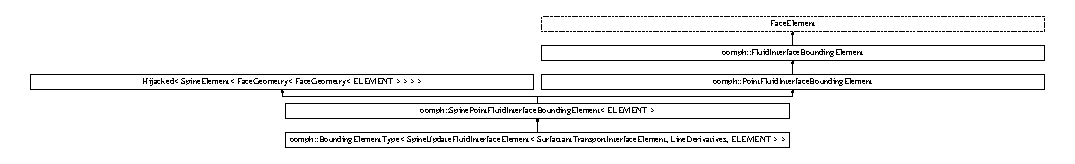
\includegraphics[height=1.752190cm]{classoomph_1_1BoundingElementType_3_01SpineUpdateFluidInterfaceElement_3_01SurfactantTransportIn1a79ed5e636f8826f4a8a00ba9f037b4}
\end{center}
\end{figure}
\subsection*{Public Member Functions}
\begin{DoxyCompactItemize}
\item 
\hyperlink{classoomph_1_1BoundingElementType_3_01SpineUpdateFluidInterfaceElement_3_01SurfactantTransportIn1a79ed5e636f8826f4a8a00ba9f037b4_a101abb5e7f32b95198b31e5dd6a6a1d0}{Bounding\+Element\+Type} ()
\end{DoxyCompactItemize}
\subsection*{Additional Inherited Members}


\subsection{Detailed Description}
\subsubsection*{template$<$class E\+L\+E\+M\+E\+NT$>$\newline
class oomph\+::\+Bounding\+Element\+Type$<$ Spine\+Update\+Fluid\+Interface\+Element$<$ Surfactant\+Transport\+Interface\+Element, Line\+Derivatives, E\+L\+E\+M\+E\+N\+T $>$ $>$}



Definition at line 218 of file surfactant\+\_\+transport\+\_\+elements.\+h.



\subsection{Constructor \& Destructor Documentation}
\mbox{\Hypertarget{classoomph_1_1BoundingElementType_3_01SpineUpdateFluidInterfaceElement_3_01SurfactantTransportIn1a79ed5e636f8826f4a8a00ba9f037b4_a101abb5e7f32b95198b31e5dd6a6a1d0}\label{classoomph_1_1BoundingElementType_3_01SpineUpdateFluidInterfaceElement_3_01SurfactantTransportIn1a79ed5e636f8826f4a8a00ba9f037b4_a101abb5e7f32b95198b31e5dd6a6a1d0}} 
\index{oomph\+::\+Bounding\+Element\+Type$<$ Spine\+Update\+Fluid\+Interface\+Element$<$ Surfactant\+Transport\+Interface\+Element, Line\+Derivatives, E\+L\+E\+M\+E\+N\+T $>$ $>$@{oomph\+::\+Bounding\+Element\+Type$<$ Spine\+Update\+Fluid\+Interface\+Element$<$ Surfactant\+Transport\+Interface\+Element, Line\+Derivatives, E\+L\+E\+M\+E\+N\+T $>$ $>$}!Bounding\+Element\+Type@{Bounding\+Element\+Type}}
\index{Bounding\+Element\+Type@{Bounding\+Element\+Type}!oomph\+::\+Bounding\+Element\+Type$<$ Spine\+Update\+Fluid\+Interface\+Element$<$ Surfactant\+Transport\+Interface\+Element, Line\+Derivatives, E\+L\+E\+M\+E\+N\+T $>$ $>$@{oomph\+::\+Bounding\+Element\+Type$<$ Spine\+Update\+Fluid\+Interface\+Element$<$ Surfactant\+Transport\+Interface\+Element, Line\+Derivatives, E\+L\+E\+M\+E\+N\+T $>$ $>$}}
\subsubsection{\texorpdfstring{Bounding\+Element\+Type()}{BoundingElementType()}}
{\footnotesize\ttfamily template$<$class E\+L\+E\+M\+E\+NT $>$ \\
\hyperlink{classoomph_1_1BoundingElementType}{oomph\+::\+Bounding\+Element\+Type}$<$ \hyperlink{classoomph_1_1SpineUpdateFluidInterfaceElement}{Spine\+Update\+Fluid\+Interface\+Element}$<$ \hyperlink{classoomph_1_1SurfactantTransportInterfaceElement}{Surfactant\+Transport\+Interface\+Element}, \hyperlink{classoomph_1_1LineDerivatives}{Line\+Derivatives}, E\+L\+E\+M\+E\+NT $>$ $>$\+::\hyperlink{classoomph_1_1BoundingElementType}{Bounding\+Element\+Type} (\begin{DoxyParamCaption}{ }\end{DoxyParamCaption})\hspace{0.3cm}{\ttfamily [inline]}}



Definition at line 225 of file surfactant\+\_\+transport\+\_\+elements.\+h.



The documentation for this class was generated from the following file\+:\begin{DoxyCompactItemize}
\item 
\hyperlink{surfactant__transport__elements_8h}{surfactant\+\_\+transport\+\_\+elements.\+h}\end{DoxyCompactItemize}

\hypertarget{classoomph_1_1BoundingElementType_3_01SpineUpdateFluidInterfaceElement_3_01SurfactantTransportIn0aa155ddfcfcc4520e061f144b3ee14d}{}\section{oomph\+:\+:Bounding\+Element\+Type$<$ Spine\+Update\+Fluid\+Interface\+Element$<$ Surfactant\+Transport\+Interface\+Element, Surface\+Derivatives, E\+L\+E\+M\+E\+NT $>$ $>$ Class Template Reference}
\label{classoomph_1_1BoundingElementType_3_01SpineUpdateFluidInterfaceElement_3_01SurfactantTransportIn0aa155ddfcfcc4520e061f144b3ee14d}\index{oomph\+::\+Bounding\+Element\+Type$<$ Spine\+Update\+Fluid\+Interface\+Element$<$ Surfactant\+Transport\+Interface\+Element, Surface\+Derivatives, E\+L\+E\+M\+E\+N\+T $>$ $>$@{oomph\+::\+Bounding\+Element\+Type$<$ Spine\+Update\+Fluid\+Interface\+Element$<$ Surfactant\+Transport\+Interface\+Element, Surface\+Derivatives, E\+L\+E\+M\+E\+N\+T $>$ $>$}}


{\ttfamily \#include $<$surfactant\+\_\+transport\+\_\+elements.\+h$>$}

Inheritance diagram for oomph\+:\+:Bounding\+Element\+Type$<$ Spine\+Update\+Fluid\+Interface\+Element$<$ Surfactant\+Transport\+Interface\+Element, Surface\+Derivatives, E\+L\+E\+M\+E\+NT $>$ $>$\+:\begin{figure}[H]
\begin{center}
\leavevmode
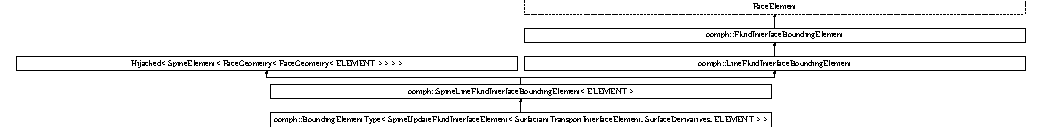
\includegraphics[height=1.092683cm]{classoomph_1_1BoundingElementType_3_01SpineUpdateFluidInterfaceElement_3_01SurfactantTransportIn0aa155ddfcfcc4520e061f144b3ee14d}
\end{center}
\end{figure}
\subsection*{Public Member Functions}
\begin{DoxyCompactItemize}
\item 
\hyperlink{classoomph_1_1BoundingElementType_3_01SpineUpdateFluidInterfaceElement_3_01SurfactantTransportIn0aa155ddfcfcc4520e061f144b3ee14d_a91a5b9d653a80f4ae5cd871b17e21936}{Bounding\+Element\+Type} ()
\end{DoxyCompactItemize}
\subsection*{Additional Inherited Members}


\subsection{Detailed Description}
\subsubsection*{template$<$class E\+L\+E\+M\+E\+NT$>$\newline
class oomph\+::\+Bounding\+Element\+Type$<$ Spine\+Update\+Fluid\+Interface\+Element$<$ Surfactant\+Transport\+Interface\+Element, Surface\+Derivatives, E\+L\+E\+M\+E\+N\+T $>$ $>$}



Definition at line 307 of file surfactant\+\_\+transport\+\_\+elements.\+h.



\subsection{Constructor \& Destructor Documentation}
\mbox{\Hypertarget{classoomph_1_1BoundingElementType_3_01SpineUpdateFluidInterfaceElement_3_01SurfactantTransportIn0aa155ddfcfcc4520e061f144b3ee14d_a91a5b9d653a80f4ae5cd871b17e21936}\label{classoomph_1_1BoundingElementType_3_01SpineUpdateFluidInterfaceElement_3_01SurfactantTransportIn0aa155ddfcfcc4520e061f144b3ee14d_a91a5b9d653a80f4ae5cd871b17e21936}} 
\index{oomph\+::\+Bounding\+Element\+Type$<$ Spine\+Update\+Fluid\+Interface\+Element$<$ Surfactant\+Transport\+Interface\+Element, Surface\+Derivatives, E\+L\+E\+M\+E\+N\+T $>$ $>$@{oomph\+::\+Bounding\+Element\+Type$<$ Spine\+Update\+Fluid\+Interface\+Element$<$ Surfactant\+Transport\+Interface\+Element, Surface\+Derivatives, E\+L\+E\+M\+E\+N\+T $>$ $>$}!Bounding\+Element\+Type@{Bounding\+Element\+Type}}
\index{Bounding\+Element\+Type@{Bounding\+Element\+Type}!oomph\+::\+Bounding\+Element\+Type$<$ Spine\+Update\+Fluid\+Interface\+Element$<$ Surfactant\+Transport\+Interface\+Element, Surface\+Derivatives, E\+L\+E\+M\+E\+N\+T $>$ $>$@{oomph\+::\+Bounding\+Element\+Type$<$ Spine\+Update\+Fluid\+Interface\+Element$<$ Surfactant\+Transport\+Interface\+Element, Surface\+Derivatives, E\+L\+E\+M\+E\+N\+T $>$ $>$}}
\subsubsection{\texorpdfstring{Bounding\+Element\+Type()}{BoundingElementType()}}
{\footnotesize\ttfamily template$<$class E\+L\+E\+M\+E\+NT $>$ \\
\hyperlink{classoomph_1_1BoundingElementType}{oomph\+::\+Bounding\+Element\+Type}$<$ \hyperlink{classoomph_1_1SpineUpdateFluidInterfaceElement}{Spine\+Update\+Fluid\+Interface\+Element}$<$ \hyperlink{classoomph_1_1SurfactantTransportInterfaceElement}{Surfactant\+Transport\+Interface\+Element}, \hyperlink{classoomph_1_1SurfaceDerivatives}{Surface\+Derivatives}, E\+L\+E\+M\+E\+NT $>$ $>$\+::\hyperlink{classoomph_1_1BoundingElementType}{Bounding\+Element\+Type} (\begin{DoxyParamCaption}{ }\end{DoxyParamCaption})\hspace{0.3cm}{\ttfamily [inline]}}



Definition at line 314 of file surfactant\+\_\+transport\+\_\+elements.\+h.



The documentation for this class was generated from the following file\+:\begin{DoxyCompactItemize}
\item 
\hyperlink{surfactant__transport__elements_8h}{surfactant\+\_\+transport\+\_\+elements.\+h}\end{DoxyCompactItemize}

\hypertarget{classoomph_1_1ElasticAxisymmetricFluidInterfaceElement}{}\section{oomph\+:\+:Elastic\+Axisymmetric\+Fluid\+Interface\+Element$<$ E\+L\+E\+M\+E\+NT $>$ Class Template Reference}
\label{classoomph_1_1ElasticAxisymmetricFluidInterfaceElement}\index{oomph\+::\+Elastic\+Axisymmetric\+Fluid\+Interface\+Element$<$ E\+L\+E\+M\+E\+N\+T $>$@{oomph\+::\+Elastic\+Axisymmetric\+Fluid\+Interface\+Element$<$ E\+L\+E\+M\+E\+N\+T $>$}}


Specialise the Elastic update case to axisymmetric equations.  




{\ttfamily \#include $<$specific\+\_\+node\+\_\+update\+\_\+interface\+\_\+elements.\+h$>$}

Inheritance diagram for oomph\+:\+:Elastic\+Axisymmetric\+Fluid\+Interface\+Element$<$ E\+L\+E\+M\+E\+NT $>$\+:\begin{figure}[H]
\begin{center}
\leavevmode
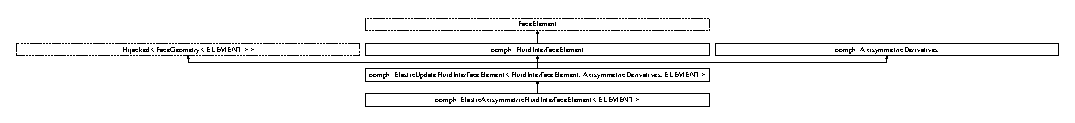
\includegraphics[height=1.202362cm]{classoomph_1_1ElasticAxisymmetricFluidInterfaceElement}
\end{center}
\end{figure}
\subsection*{Public Member Functions}
\begin{DoxyCompactItemize}
\item 
\hyperlink{classoomph_1_1ElasticAxisymmetricFluidInterfaceElement_a9cb419f11aa4504bca4b6a9c40cca505}{Elastic\+Axisymmetric\+Fluid\+Interface\+Element} (Finite\+Element $\ast$const \&element\+\_\+pt, const int \&face\+\_\+index, const unsigned \&id=0)
\end{DoxyCompactItemize}
\subsection*{Additional Inherited Members}


\subsection{Detailed Description}
\subsubsection*{template$<$class E\+L\+E\+M\+E\+NT$>$\newline
class oomph\+::\+Elastic\+Axisymmetric\+Fluid\+Interface\+Element$<$ E\+L\+E\+M\+E\+N\+T $>$}

Specialise the Elastic update case to axisymmetric equations. 

Definition at line 1095 of file specific\+\_\+node\+\_\+update\+\_\+interface\+\_\+elements.\+h.



\subsection{Constructor \& Destructor Documentation}
\mbox{\Hypertarget{classoomph_1_1ElasticAxisymmetricFluidInterfaceElement_a9cb419f11aa4504bca4b6a9c40cca505}\label{classoomph_1_1ElasticAxisymmetricFluidInterfaceElement_a9cb419f11aa4504bca4b6a9c40cca505}} 
\index{oomph\+::\+Elastic\+Axisymmetric\+Fluid\+Interface\+Element@{oomph\+::\+Elastic\+Axisymmetric\+Fluid\+Interface\+Element}!Elastic\+Axisymmetric\+Fluid\+Interface\+Element@{Elastic\+Axisymmetric\+Fluid\+Interface\+Element}}
\index{Elastic\+Axisymmetric\+Fluid\+Interface\+Element@{Elastic\+Axisymmetric\+Fluid\+Interface\+Element}!oomph\+::\+Elastic\+Axisymmetric\+Fluid\+Interface\+Element@{oomph\+::\+Elastic\+Axisymmetric\+Fluid\+Interface\+Element}}
\subsubsection{\texorpdfstring{Elastic\+Axisymmetric\+Fluid\+Interface\+Element()}{ElasticAxisymmetricFluidInterfaceElement()}}
{\footnotesize\ttfamily template$<$class E\+L\+E\+M\+E\+NT $>$ \\
\hyperlink{classoomph_1_1ElasticAxisymmetricFluidInterfaceElement}{oomph\+::\+Elastic\+Axisymmetric\+Fluid\+Interface\+Element}$<$ E\+L\+E\+M\+E\+NT $>$\+::\hyperlink{classoomph_1_1ElasticAxisymmetricFluidInterfaceElement}{Elastic\+Axisymmetric\+Fluid\+Interface\+Element} (\begin{DoxyParamCaption}\item[{Finite\+Element $\ast$const \&}]{element\+\_\+pt,  }\item[{const int \&}]{face\+\_\+index,  }\item[{const unsigned \&}]{id = {\ttfamily 0} }\end{DoxyParamCaption})\hspace{0.3cm}{\ttfamily [inline]}}



Definition at line 1101 of file specific\+\_\+node\+\_\+update\+\_\+interface\+\_\+elements.\+h.



The documentation for this class was generated from the following file\+:\begin{DoxyCompactItemize}
\item 
\hyperlink{specific__node__update__interface__elements_8h}{specific\+\_\+node\+\_\+update\+\_\+interface\+\_\+elements.\+h}\end{DoxyCompactItemize}

\hypertarget{classoomph_1_1ElasticAxisymmetricSurfactantTransportInterfaceElement}{}\section{oomph\+:\+:Elastic\+Axisymmetric\+Surfactant\+Transport\+Interface\+Element$<$ E\+L\+E\+M\+E\+NT $>$ Class Template Reference}
\label{classoomph_1_1ElasticAxisymmetricSurfactantTransportInterfaceElement}\index{oomph\+::\+Elastic\+Axisymmetric\+Surfactant\+Transport\+Interface\+Element$<$ E\+L\+E\+M\+E\+N\+T $>$@{oomph\+::\+Elastic\+Axisymmetric\+Surfactant\+Transport\+Interface\+Element$<$ E\+L\+E\+M\+E\+N\+T $>$}}


Specialise to the Axisymmetric geometry.  




{\ttfamily \#include $<$surfactant\+\_\+transport\+\_\+elements.\+h$>$}

Inheritance diagram for oomph\+:\+:Elastic\+Axisymmetric\+Surfactant\+Transport\+Interface\+Element$<$ E\+L\+E\+M\+E\+NT $>$\+:\begin{figure}[H]
\begin{center}
\leavevmode
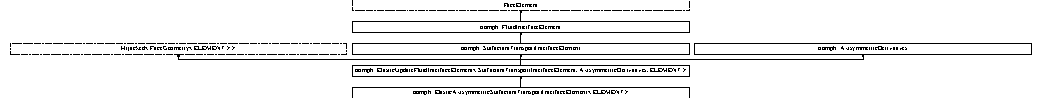
\includegraphics[height=1.390071cm]{classoomph_1_1ElasticAxisymmetricSurfactantTransportInterfaceElement}
\end{center}
\end{figure}
\subsection*{Public Member Functions}
\begin{DoxyCompactItemize}
\item 
\hyperlink{classoomph_1_1ElasticAxisymmetricSurfactantTransportInterfaceElement_a7e0f4dbf25bf0556a2675e599eeb6365}{Elastic\+Axisymmetric\+Surfactant\+Transport\+Interface\+Element} (\hyperlink{classoomph_1_1FiniteElement}{Finite\+Element} $\ast$const \&element\+\_\+pt, const int \&\hyperlink{classoomph_1_1FaceElement_a478d577ac6db67ecc80f1f02ae3ab170}{face\+\_\+index})
\end{DoxyCompactItemize}
\subsection*{Additional Inherited Members}


\subsection{Detailed Description}
\subsubsection*{template$<$class E\+L\+E\+M\+E\+NT$>$\newline
class oomph\+::\+Elastic\+Axisymmetric\+Surfactant\+Transport\+Interface\+Element$<$ E\+L\+E\+M\+E\+N\+T $>$}

Specialise to the Axisymmetric geometry. 

Definition at line 261 of file surfactant\+\_\+transport\+\_\+elements.\+h.



\subsection{Constructor \& Destructor Documentation}
\mbox{\Hypertarget{classoomph_1_1ElasticAxisymmetricSurfactantTransportInterfaceElement_a7e0f4dbf25bf0556a2675e599eeb6365}\label{classoomph_1_1ElasticAxisymmetricSurfactantTransportInterfaceElement_a7e0f4dbf25bf0556a2675e599eeb6365}} 
\index{oomph\+::\+Elastic\+Axisymmetric\+Surfactant\+Transport\+Interface\+Element@{oomph\+::\+Elastic\+Axisymmetric\+Surfactant\+Transport\+Interface\+Element}!Elastic\+Axisymmetric\+Surfactant\+Transport\+Interface\+Element@{Elastic\+Axisymmetric\+Surfactant\+Transport\+Interface\+Element}}
\index{Elastic\+Axisymmetric\+Surfactant\+Transport\+Interface\+Element@{Elastic\+Axisymmetric\+Surfactant\+Transport\+Interface\+Element}!oomph\+::\+Elastic\+Axisymmetric\+Surfactant\+Transport\+Interface\+Element@{oomph\+::\+Elastic\+Axisymmetric\+Surfactant\+Transport\+Interface\+Element}}
\subsubsection{\texorpdfstring{Elastic\+Axisymmetric\+Surfactant\+Transport\+Interface\+Element()}{ElasticAxisymmetricSurfactantTransportInterfaceElement()}}
{\footnotesize\ttfamily template$<$class E\+L\+E\+M\+E\+NT $>$ \\
\hyperlink{classoomph_1_1ElasticAxisymmetricSurfactantTransportInterfaceElement}{oomph\+::\+Elastic\+Axisymmetric\+Surfactant\+Transport\+Interface\+Element}$<$ E\+L\+E\+M\+E\+NT $>$\+::\hyperlink{classoomph_1_1ElasticAxisymmetricSurfactantTransportInterfaceElement}{Elastic\+Axisymmetric\+Surfactant\+Transport\+Interface\+Element} (\begin{DoxyParamCaption}\item[{\hyperlink{classoomph_1_1FiniteElement}{Finite\+Element} $\ast$const \&}]{element\+\_\+pt,  }\item[{const int \&}]{face\+\_\+index }\end{DoxyParamCaption})\hspace{0.3cm}{\ttfamily [inline]}}



Definition at line 267 of file surfactant\+\_\+transport\+\_\+elements.\+h.



The documentation for this class was generated from the following file\+:\begin{DoxyCompactItemize}
\item 
\hyperlink{surfactant__transport__elements_8h}{surfactant\+\_\+transport\+\_\+elements.\+h}\end{DoxyCompactItemize}

\hypertarget{classoomph_1_1ElasticAxisymmetricVolumeConstraintBoundingElement}{}\section{oomph\+:\+:Elastic\+Axisymmetric\+Volume\+Constraint\+Bounding\+Element$<$ E\+L\+E\+M\+E\+NT $>$ Class Template Reference}
\label{classoomph_1_1ElasticAxisymmetricVolumeConstraintBoundingElement}\index{oomph\+::\+Elastic\+Axisymmetric\+Volume\+Constraint\+Bounding\+Element$<$ E\+L\+E\+M\+E\+N\+T $>$@{oomph\+::\+Elastic\+Axisymmetric\+Volume\+Constraint\+Bounding\+Element$<$ E\+L\+E\+M\+E\+N\+T $>$}}


{\ttfamily \#include $<$constrained\+\_\+volume\+\_\+elements.\+h$>$}

Inheritance diagram for oomph\+:\+:Elastic\+Axisymmetric\+Volume\+Constraint\+Bounding\+Element$<$ E\+L\+E\+M\+E\+NT $>$\+:\begin{figure}[H]
\begin{center}
\leavevmode
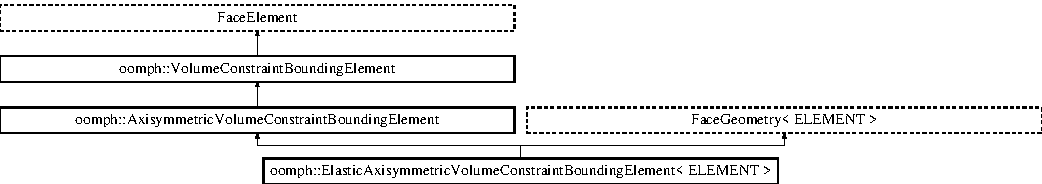
\includegraphics[height=2.477876cm]{classoomph_1_1ElasticAxisymmetricVolumeConstraintBoundingElement}
\end{center}
\end{figure}
\subsection*{Public Member Functions}
\begin{DoxyCompactItemize}
\item 
\hyperlink{classoomph_1_1ElasticAxisymmetricVolumeConstraintBoundingElement_a533376e1f314fabc4c014f9c7547f5e8}{Elastic\+Axisymmetric\+Volume\+Constraint\+Bounding\+Element} (Finite\+Element $\ast$const \&element\+\_\+pt, const int \&face\+\_\+index)
\begin{DoxyCompactList}\small\item\em Contructor\+: Specify bulk element and index of face to which this face element is to be attached. \end{DoxyCompactList}\item 
void \hyperlink{classoomph_1_1ElasticAxisymmetricVolumeConstraintBoundingElement_adc7f5296f867251fe4b97b01f40c11e7}{fill\+\_\+in\+\_\+contribution\+\_\+to\+\_\+jacobian} (Vector$<$ double $>$ \&residuals, Dense\+Matrix$<$ double $>$ \&jacobian)
\item 
double \hyperlink{classoomph_1_1ElasticAxisymmetricVolumeConstraintBoundingElement_a8fe8843e542a626dd374cc4cd6850bcb}{zeta\+\_\+nodal} (const unsigned \&n, const unsigned \&k, const unsigned \&i) const
\begin{DoxyCompactList}\small\item\em The \char`\"{}global\char`\"{} intrinsic coordinate of the element when viewed as part of a geometric object should be given by the Face\+Element representation, by default. \end{DoxyCompactList}\end{DoxyCompactItemize}
\subsection*{Additional Inherited Members}


\subsection{Detailed Description}
\subsubsection*{template$<$class E\+L\+E\+M\+E\+NT$>$\newline
class oomph\+::\+Elastic\+Axisymmetric\+Volume\+Constraint\+Bounding\+Element$<$ E\+L\+E\+M\+E\+N\+T $>$}

The axisymmetric (one-\/dimensional) interface elements that allow imposition of a volume constraint specialised for the case when the nodal positions of the bulk elements are treated as solid degrees of freedom. To enforce that a fluid volume has a certain volume, attach these elements to all faces of the (2D axisymmetric) bulk fluid elements (of type E\+L\+E\+M\+E\+NT) that bound that region and then specify the \char`\"{}pressure\char`\"{} value that is traded for the constraint. 

Definition at line 612 of file constrained\+\_\+volume\+\_\+elements.\+h.



\subsection{Constructor \& Destructor Documentation}
\mbox{\Hypertarget{classoomph_1_1ElasticAxisymmetricVolumeConstraintBoundingElement_a533376e1f314fabc4c014f9c7547f5e8}\label{classoomph_1_1ElasticAxisymmetricVolumeConstraintBoundingElement_a533376e1f314fabc4c014f9c7547f5e8}} 
\index{oomph\+::\+Elastic\+Axisymmetric\+Volume\+Constraint\+Bounding\+Element@{oomph\+::\+Elastic\+Axisymmetric\+Volume\+Constraint\+Bounding\+Element}!Elastic\+Axisymmetric\+Volume\+Constraint\+Bounding\+Element@{Elastic\+Axisymmetric\+Volume\+Constraint\+Bounding\+Element}}
\index{Elastic\+Axisymmetric\+Volume\+Constraint\+Bounding\+Element@{Elastic\+Axisymmetric\+Volume\+Constraint\+Bounding\+Element}!oomph\+::\+Elastic\+Axisymmetric\+Volume\+Constraint\+Bounding\+Element@{oomph\+::\+Elastic\+Axisymmetric\+Volume\+Constraint\+Bounding\+Element}}
\subsubsection{\texorpdfstring{Elastic\+Axisymmetric\+Volume\+Constraint\+Bounding\+Element()}{ElasticAxisymmetricVolumeConstraintBoundingElement()}}
{\footnotesize\ttfamily template$<$class E\+L\+E\+M\+E\+NT $>$ \\
\hyperlink{classoomph_1_1ElasticAxisymmetricVolumeConstraintBoundingElement}{oomph\+::\+Elastic\+Axisymmetric\+Volume\+Constraint\+Bounding\+Element}$<$ E\+L\+E\+M\+E\+NT $>$\+::\hyperlink{classoomph_1_1ElasticAxisymmetricVolumeConstraintBoundingElement}{Elastic\+Axisymmetric\+Volume\+Constraint\+Bounding\+Element} (\begin{DoxyParamCaption}\item[{Finite\+Element $\ast$const \&}]{element\+\_\+pt,  }\item[{const int \&}]{face\+\_\+index }\end{DoxyParamCaption})\hspace{0.3cm}{\ttfamily [inline]}}



Contructor\+: Specify bulk element and index of face to which this face element is to be attached. 



Definition at line 621 of file constrained\+\_\+volume\+\_\+elements.\+h.



\subsection{Member Function Documentation}
\mbox{\Hypertarget{classoomph_1_1ElasticAxisymmetricVolumeConstraintBoundingElement_adc7f5296f867251fe4b97b01f40c11e7}\label{classoomph_1_1ElasticAxisymmetricVolumeConstraintBoundingElement_adc7f5296f867251fe4b97b01f40c11e7}} 
\index{oomph\+::\+Elastic\+Axisymmetric\+Volume\+Constraint\+Bounding\+Element@{oomph\+::\+Elastic\+Axisymmetric\+Volume\+Constraint\+Bounding\+Element}!fill\+\_\+in\+\_\+contribution\+\_\+to\+\_\+jacobian@{fill\+\_\+in\+\_\+contribution\+\_\+to\+\_\+jacobian}}
\index{fill\+\_\+in\+\_\+contribution\+\_\+to\+\_\+jacobian@{fill\+\_\+in\+\_\+contribution\+\_\+to\+\_\+jacobian}!oomph\+::\+Elastic\+Axisymmetric\+Volume\+Constraint\+Bounding\+Element@{oomph\+::\+Elastic\+Axisymmetric\+Volume\+Constraint\+Bounding\+Element}}
\subsubsection{\texorpdfstring{fill\+\_\+in\+\_\+contribution\+\_\+to\+\_\+jacobian()}{fill\_in\_contribution\_to\_jacobian()}}
{\footnotesize\ttfamily template$<$class E\+L\+E\+M\+E\+NT $>$ \\
void \hyperlink{classoomph_1_1ElasticAxisymmetricVolumeConstraintBoundingElement}{oomph\+::\+Elastic\+Axisymmetric\+Volume\+Constraint\+Bounding\+Element}$<$ E\+L\+E\+M\+E\+NT $>$\+::fill\+\_\+in\+\_\+contribution\+\_\+to\+\_\+jacobian (\begin{DoxyParamCaption}\item[{Vector$<$ double $>$ \&}]{residuals,  }\item[{Dense\+Matrix$<$ double $>$ \&}]{jacobian }\end{DoxyParamCaption})\hspace{0.3cm}{\ttfamily [inline]}}

Fill in contribution to residuals and Jacobian. This is specific to solid-\/based elements in which derivatives w.\+r.\+t. to nodal positions are evaluated by finite differencing 

Definition at line 635 of file constrained\+\_\+volume\+\_\+elements.\+h.

\mbox{\Hypertarget{classoomph_1_1ElasticAxisymmetricVolumeConstraintBoundingElement_a8fe8843e542a626dd374cc4cd6850bcb}\label{classoomph_1_1ElasticAxisymmetricVolumeConstraintBoundingElement_a8fe8843e542a626dd374cc4cd6850bcb}} 
\index{oomph\+::\+Elastic\+Axisymmetric\+Volume\+Constraint\+Bounding\+Element@{oomph\+::\+Elastic\+Axisymmetric\+Volume\+Constraint\+Bounding\+Element}!zeta\+\_\+nodal@{zeta\+\_\+nodal}}
\index{zeta\+\_\+nodal@{zeta\+\_\+nodal}!oomph\+::\+Elastic\+Axisymmetric\+Volume\+Constraint\+Bounding\+Element@{oomph\+::\+Elastic\+Axisymmetric\+Volume\+Constraint\+Bounding\+Element}}
\subsubsection{\texorpdfstring{zeta\+\_\+nodal()}{zeta\_nodal()}}
{\footnotesize\ttfamily template$<$class E\+L\+E\+M\+E\+NT $>$ \\
double \hyperlink{classoomph_1_1ElasticAxisymmetricVolumeConstraintBoundingElement}{oomph\+::\+Elastic\+Axisymmetric\+Volume\+Constraint\+Bounding\+Element}$<$ E\+L\+E\+M\+E\+NT $>$\+::zeta\+\_\+nodal (\begin{DoxyParamCaption}\item[{const unsigned \&}]{n,  }\item[{const unsigned \&}]{k,  }\item[{const unsigned \&}]{i }\end{DoxyParamCaption}) const\hspace{0.3cm}{\ttfamily [inline]}}



The \char`\"{}global\char`\"{} intrinsic coordinate of the element when viewed as part of a geometric object should be given by the Face\+Element representation, by default. 



Definition at line 649 of file constrained\+\_\+volume\+\_\+elements.\+h.



The documentation for this class was generated from the following file\+:\begin{DoxyCompactItemize}
\item 
\hyperlink{constrained__volume__elements_8h}{constrained\+\_\+volume\+\_\+elements.\+h}\end{DoxyCompactItemize}

\hypertarget{classoomph_1_1ElasticLineFluidInterfaceBoundingElement}{}\section{oomph\+:\+:Elastic\+Line\+Fluid\+Interface\+Bounding\+Element$<$ E\+L\+E\+M\+E\+NT $>$ Class Template Reference}
\label{classoomph_1_1ElasticLineFluidInterfaceBoundingElement}\index{oomph\+::\+Elastic\+Line\+Fluid\+Interface\+Bounding\+Element$<$ E\+L\+E\+M\+E\+N\+T $>$@{oomph\+::\+Elastic\+Line\+Fluid\+Interface\+Bounding\+Element$<$ E\+L\+E\+M\+E\+N\+T $>$}}


Pseudo-\/elasticity version of the \hyperlink{classoomph_1_1LineFluidInterfaceBoundingElement}{Line\+Fluid\+Interface\+Bounding\+Element}.  




{\ttfamily \#include $<$specific\+\_\+node\+\_\+update\+\_\+interface\+\_\+elements.\+h$>$}

Inheritance diagram for oomph\+:\+:Elastic\+Line\+Fluid\+Interface\+Bounding\+Element$<$ E\+L\+E\+M\+E\+NT $>$\+:\begin{figure}[H]
\begin{center}
\leavevmode
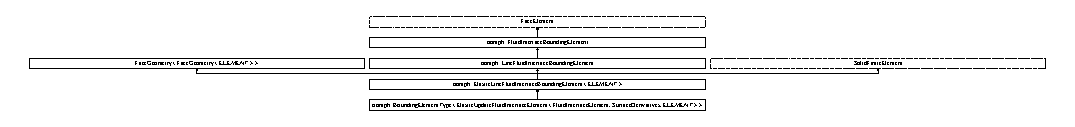
\includegraphics[height=1.322537cm]{classoomph_1_1ElasticLineFluidInterfaceBoundingElement}
\end{center}
\end{figure}
\subsection*{Public Member Functions}
\begin{DoxyCompactItemize}
\item 
void \hyperlink{classoomph_1_1ElasticLineFluidInterfaceBoundingElement_a524b359509676cd429729e0dde59da92}{set\+\_\+lagrange\+\_\+index} (const \hyperlink{classoomph_1_1Vector}{Vector}$<$ unsigned $>$ \&lagrange\+\_\+index)
\begin{DoxyCompactList}\small\item\em Set the Id. \end{DoxyCompactList}\item 
\hyperlink{classoomph_1_1ElasticLineFluidInterfaceBoundingElement_ad531b7e5debaecc74d64755c82bbc17d}{Elastic\+Line\+Fluid\+Interface\+Bounding\+Element} ()
\begin{DoxyCompactList}\small\item\em Constructor. \end{DoxyCompactList}\item 
double \hyperlink{classoomph_1_1ElasticLineFluidInterfaceBoundingElement_a1d8a7213d7bd2826bc59af770f66f402}{zeta\+\_\+nodal} (const unsigned \&n, const unsigned \&k, const unsigned \&\hyperlink{cfortran_8h_adb50e893b86b3e55e751a42eab3cba82}{i}) const
\begin{DoxyCompactList}\small\item\em Specify the value of nodal zeta from the face geometry The \char`\"{}global\char`\"{} intrinsic coordinate of the element when viewed as part of a geometric object should be given by the \hyperlink{classoomph_1_1FaceElement}{Face\+Element} representation, by default. \end{DoxyCompactList}\item 
void \hyperlink{classoomph_1_1ElasticLineFluidInterfaceBoundingElement_a50444fef924185e8d462238045e24543}{output} (std\+::ostream \&outfile)
\begin{DoxyCompactList}\small\item\em Overload the output function. \end{DoxyCompactList}\item 
void \hyperlink{classoomph_1_1ElasticLineFluidInterfaceBoundingElement_a7a0df1419f28df0351ed1c5e05f8f751}{output} (std\+::ostream \&outfile, const unsigned \&n\+\_\+plot)
\begin{DoxyCompactList}\small\item\em Output the element. \end{DoxyCompactList}\item 
void \hyperlink{classoomph_1_1ElasticLineFluidInterfaceBoundingElement_a0979784b94ab8285a964ab14077b8320}{output} (F\+I\+LE $\ast$file\+\_\+pt)
\begin{DoxyCompactList}\small\item\em Overload the C-\/style output function. \end{DoxyCompactList}\item 
void \hyperlink{classoomph_1_1ElasticLineFluidInterfaceBoundingElement_a6e4c4d356c7d66f6b5ec4c7a375ecc91}{output} (F\+I\+LE $\ast$file\+\_\+pt, const unsigned \&n\+\_\+plot)
\begin{DoxyCompactList}\small\item\em C-\/style Output function. \end{DoxyCompactList}\item 
void \hyperlink{classoomph_1_1ElasticLineFluidInterfaceBoundingElement_a71b23e3ad49d5137ca4a7f654f828077}{fill\+\_\+in\+\_\+contribution\+\_\+to\+\_\+jacobian} (\hyperlink{classoomph_1_1Vector}{Vector}$<$ double $>$ \&residuals, \hyperlink{classoomph_1_1DenseMatrix}{Dense\+Matrix}$<$ double $>$ \&jacobian)
\begin{DoxyCompactList}\small\item\em Calculate the elemental residual vector and Jacobian. \end{DoxyCompactList}\item 
int \hyperlink{classoomph_1_1ElasticLineFluidInterfaceBoundingElement_a0f3d4bdd756165d6a2225f5b13eac005}{kinematic\+\_\+local\+\_\+eqn} (const unsigned \&n)
\begin{DoxyCompactList}\small\item\em Local eqn number of kinematic bc associated with local node n. \end{DoxyCompactList}\end{DoxyCompactItemize}
\subsection*{Private Attributes}
\begin{DoxyCompactItemize}
\item 
\hyperlink{classoomph_1_1Vector}{Vector}$<$ unsigned $>$ \hyperlink{classoomph_1_1ElasticLineFluidInterfaceBoundingElement_ab60624e63f1ef1b59d191a83b16eb1de}{Lagrange\+\_\+index}
\begin{DoxyCompactList}\small\item\em Short Storage for the index of Lagrange multiplier. \end{DoxyCompactList}\end{DoxyCompactItemize}
\subsection*{Additional Inherited Members}


\subsection{Detailed Description}
\subsubsection*{template$<$class E\+L\+E\+M\+E\+NT$>$\newline
class oomph\+::\+Elastic\+Line\+Fluid\+Interface\+Bounding\+Element$<$ E\+L\+E\+M\+E\+N\+T $>$}

Pseudo-\/elasticity version of the \hyperlink{classoomph_1_1LineFluidInterfaceBoundingElement}{Line\+Fluid\+Interface\+Bounding\+Element}. 

Definition at line 991 of file specific\+\_\+node\+\_\+update\+\_\+interface\+\_\+elements.\+h.



\subsection{Constructor \& Destructor Documentation}
\mbox{\Hypertarget{classoomph_1_1ElasticLineFluidInterfaceBoundingElement_ad531b7e5debaecc74d64755c82bbc17d}\label{classoomph_1_1ElasticLineFluidInterfaceBoundingElement_ad531b7e5debaecc74d64755c82bbc17d}} 
\index{oomph\+::\+Elastic\+Line\+Fluid\+Interface\+Bounding\+Element@{oomph\+::\+Elastic\+Line\+Fluid\+Interface\+Bounding\+Element}!Elastic\+Line\+Fluid\+Interface\+Bounding\+Element@{Elastic\+Line\+Fluid\+Interface\+Bounding\+Element}}
\index{Elastic\+Line\+Fluid\+Interface\+Bounding\+Element@{Elastic\+Line\+Fluid\+Interface\+Bounding\+Element}!oomph\+::\+Elastic\+Line\+Fluid\+Interface\+Bounding\+Element@{oomph\+::\+Elastic\+Line\+Fluid\+Interface\+Bounding\+Element}}
\subsubsection{\texorpdfstring{Elastic\+Line\+Fluid\+Interface\+Bounding\+Element()}{ElasticLineFluidInterfaceBoundingElement()}}
{\footnotesize\ttfamily template$<$class E\+L\+E\+M\+E\+NT $>$ \\
\hyperlink{classoomph_1_1ElasticLineFluidInterfaceBoundingElement}{oomph\+::\+Elastic\+Line\+Fluid\+Interface\+Bounding\+Element}$<$ E\+L\+E\+M\+E\+NT $>$\+::\hyperlink{classoomph_1_1ElasticLineFluidInterfaceBoundingElement}{Elastic\+Line\+Fluid\+Interface\+Bounding\+Element} (\begin{DoxyParamCaption}{ }\end{DoxyParamCaption})\hspace{0.3cm}{\ttfamily [inline]}}



Constructor. 



Definition at line 1007 of file specific\+\_\+node\+\_\+update\+\_\+interface\+\_\+elements.\+h.



\subsection{Member Function Documentation}
\mbox{\Hypertarget{classoomph_1_1ElasticLineFluidInterfaceBoundingElement_a71b23e3ad49d5137ca4a7f654f828077}\label{classoomph_1_1ElasticLineFluidInterfaceBoundingElement_a71b23e3ad49d5137ca4a7f654f828077}} 
\index{oomph\+::\+Elastic\+Line\+Fluid\+Interface\+Bounding\+Element@{oomph\+::\+Elastic\+Line\+Fluid\+Interface\+Bounding\+Element}!fill\+\_\+in\+\_\+contribution\+\_\+to\+\_\+jacobian@{fill\+\_\+in\+\_\+contribution\+\_\+to\+\_\+jacobian}}
\index{fill\+\_\+in\+\_\+contribution\+\_\+to\+\_\+jacobian@{fill\+\_\+in\+\_\+contribution\+\_\+to\+\_\+jacobian}!oomph\+::\+Elastic\+Line\+Fluid\+Interface\+Bounding\+Element@{oomph\+::\+Elastic\+Line\+Fluid\+Interface\+Bounding\+Element}}
\subsubsection{\texorpdfstring{fill\+\_\+in\+\_\+contribution\+\_\+to\+\_\+jacobian()}{fill\_in\_contribution\_to\_jacobian()}}
{\footnotesize\ttfamily template$<$class E\+L\+E\+M\+E\+NT $>$ \\
void \hyperlink{classoomph_1_1ElasticLineFluidInterfaceBoundingElement}{oomph\+::\+Elastic\+Line\+Fluid\+Interface\+Bounding\+Element}$<$ E\+L\+E\+M\+E\+NT $>$\+::fill\+\_\+in\+\_\+contribution\+\_\+to\+\_\+jacobian (\begin{DoxyParamCaption}\item[{\hyperlink{classoomph_1_1Vector}{Vector}$<$ double $>$ \&}]{residuals,  }\item[{\hyperlink{classoomph_1_1DenseMatrix}{Dense\+Matrix}$<$ double $>$ \&}]{jacobian }\end{DoxyParamCaption})\hspace{0.3cm}{\ttfamily [inline]}, {\ttfamily [virtual]}}



Calculate the elemental residual vector and Jacobian. 



Reimplemented from \hyperlink{classoomph_1_1GeneralisedElement_a6ae09fc0d68e4309ac1b03583d252845}{oomph\+::\+Generalised\+Element}.



Definition at line 1037 of file specific\+\_\+node\+\_\+update\+\_\+interface\+\_\+elements.\+h.

\mbox{\Hypertarget{classoomph_1_1ElasticLineFluidInterfaceBoundingElement_a0f3d4bdd756165d6a2225f5b13eac005}\label{classoomph_1_1ElasticLineFluidInterfaceBoundingElement_a0f3d4bdd756165d6a2225f5b13eac005}} 
\index{oomph\+::\+Elastic\+Line\+Fluid\+Interface\+Bounding\+Element@{oomph\+::\+Elastic\+Line\+Fluid\+Interface\+Bounding\+Element}!kinematic\+\_\+local\+\_\+eqn@{kinematic\+\_\+local\+\_\+eqn}}
\index{kinematic\+\_\+local\+\_\+eqn@{kinematic\+\_\+local\+\_\+eqn}!oomph\+::\+Elastic\+Line\+Fluid\+Interface\+Bounding\+Element@{oomph\+::\+Elastic\+Line\+Fluid\+Interface\+Bounding\+Element}}
\subsubsection{\texorpdfstring{kinematic\+\_\+local\+\_\+eqn()}{kinematic\_local\_eqn()}}
{\footnotesize\ttfamily template$<$class E\+L\+E\+M\+E\+NT $>$ \\
int \hyperlink{classoomph_1_1ElasticLineFluidInterfaceBoundingElement}{oomph\+::\+Elastic\+Line\+Fluid\+Interface\+Bounding\+Element}$<$ E\+L\+E\+M\+E\+NT $>$\+::kinematic\+\_\+local\+\_\+eqn (\begin{DoxyParamCaption}\item[{const unsigned \&}]{n }\end{DoxyParamCaption})\hspace{0.3cm}{\ttfamily [inline]}, {\ttfamily [virtual]}}



Local eqn number of kinematic bc associated with local node n. 



Implements \hyperlink{classoomph_1_1FluidInterfaceBoundingElement_a12a0a6d7c3c1c1a5a0f42a57e60eab34}{oomph\+::\+Fluid\+Interface\+Bounding\+Element}.



Definition at line 1051 of file specific\+\_\+node\+\_\+update\+\_\+interface\+\_\+elements.\+h.

\mbox{\Hypertarget{classoomph_1_1ElasticLineFluidInterfaceBoundingElement_a50444fef924185e8d462238045e24543}\label{classoomph_1_1ElasticLineFluidInterfaceBoundingElement_a50444fef924185e8d462238045e24543}} 
\index{oomph\+::\+Elastic\+Line\+Fluid\+Interface\+Bounding\+Element@{oomph\+::\+Elastic\+Line\+Fluid\+Interface\+Bounding\+Element}!output@{output}}
\index{output@{output}!oomph\+::\+Elastic\+Line\+Fluid\+Interface\+Bounding\+Element@{oomph\+::\+Elastic\+Line\+Fluid\+Interface\+Bounding\+Element}}
\subsubsection{\texorpdfstring{output()}{output()}\hspace{0.1cm}{\footnotesize\ttfamily [1/4]}}
{\footnotesize\ttfamily template$<$class E\+L\+E\+M\+E\+NT $>$ \\
void \hyperlink{classoomph_1_1ElasticLineFluidInterfaceBoundingElement}{oomph\+::\+Elastic\+Line\+Fluid\+Interface\+Bounding\+Element}$<$ E\+L\+E\+M\+E\+NT $>$\+::output (\begin{DoxyParamCaption}\item[{std\+::ostream \&}]{outfile }\end{DoxyParamCaption})\hspace{0.3cm}{\ttfamily [inline]}, {\ttfamily [virtual]}}



Overload the output function. 



Reimplemented from \hyperlink{classoomph_1_1FluidInterfaceBoundingElement_a81adc5ae89ddfa120f587c61b972622f}{oomph\+::\+Fluid\+Interface\+Bounding\+Element}.



Definition at line 1021 of file specific\+\_\+node\+\_\+update\+\_\+interface\+\_\+elements.\+h.



References oomph\+::\+Finite\+Element\+::output().

\mbox{\Hypertarget{classoomph_1_1ElasticLineFluidInterfaceBoundingElement_a7a0df1419f28df0351ed1c5e05f8f751}\label{classoomph_1_1ElasticLineFluidInterfaceBoundingElement_a7a0df1419f28df0351ed1c5e05f8f751}} 
\index{oomph\+::\+Elastic\+Line\+Fluid\+Interface\+Bounding\+Element@{oomph\+::\+Elastic\+Line\+Fluid\+Interface\+Bounding\+Element}!output@{output}}
\index{output@{output}!oomph\+::\+Elastic\+Line\+Fluid\+Interface\+Bounding\+Element@{oomph\+::\+Elastic\+Line\+Fluid\+Interface\+Bounding\+Element}}
\subsubsection{\texorpdfstring{output()}{output()}\hspace{0.1cm}{\footnotesize\ttfamily [2/4]}}
{\footnotesize\ttfamily template$<$class E\+L\+E\+M\+E\+NT $>$ \\
void \hyperlink{classoomph_1_1ElasticLineFluidInterfaceBoundingElement}{oomph\+::\+Elastic\+Line\+Fluid\+Interface\+Bounding\+Element}$<$ E\+L\+E\+M\+E\+NT $>$\+::output (\begin{DoxyParamCaption}\item[{std\+::ostream \&}]{outfile,  }\item[{const unsigned \&}]{n\+\_\+plot }\end{DoxyParamCaption})\hspace{0.3cm}{\ttfamily [inline]}, {\ttfamily [virtual]}}



Output the element. 



Reimplemented from \hyperlink{classoomph_1_1FluidInterfaceBoundingElement_af2c821d51d506221976a0c17e1615ac3}{oomph\+::\+Fluid\+Interface\+Bounding\+Element}.



Definition at line 1024 of file specific\+\_\+node\+\_\+update\+\_\+interface\+\_\+elements.\+h.



References oomph\+::\+Fluid\+Interface\+Bounding\+Element\+::output().

\mbox{\Hypertarget{classoomph_1_1ElasticLineFluidInterfaceBoundingElement_a0979784b94ab8285a964ab14077b8320}\label{classoomph_1_1ElasticLineFluidInterfaceBoundingElement_a0979784b94ab8285a964ab14077b8320}} 
\index{oomph\+::\+Elastic\+Line\+Fluid\+Interface\+Bounding\+Element@{oomph\+::\+Elastic\+Line\+Fluid\+Interface\+Bounding\+Element}!output@{output}}
\index{output@{output}!oomph\+::\+Elastic\+Line\+Fluid\+Interface\+Bounding\+Element@{oomph\+::\+Elastic\+Line\+Fluid\+Interface\+Bounding\+Element}}
\subsubsection{\texorpdfstring{output()}{output()}\hspace{0.1cm}{\footnotesize\ttfamily [3/4]}}
{\footnotesize\ttfamily template$<$class E\+L\+E\+M\+E\+NT $>$ \\
void \hyperlink{classoomph_1_1ElasticLineFluidInterfaceBoundingElement}{oomph\+::\+Elastic\+Line\+Fluid\+Interface\+Bounding\+Element}$<$ E\+L\+E\+M\+E\+NT $>$\+::output (\begin{DoxyParamCaption}\item[{F\+I\+LE $\ast$}]{file\+\_\+pt }\end{DoxyParamCaption})\hspace{0.3cm}{\ttfamily [inline]}, {\ttfamily [virtual]}}



Overload the C-\/style output function. 



Reimplemented from \hyperlink{classoomph_1_1FluidInterfaceBoundingElement_a85cc62405429744e3e3585894315cb9e}{oomph\+::\+Fluid\+Interface\+Bounding\+Element}.



Definition at line 1030 of file specific\+\_\+node\+\_\+update\+\_\+interface\+\_\+elements.\+h.



References oomph\+::\+Finite\+Element\+::output().

\mbox{\Hypertarget{classoomph_1_1ElasticLineFluidInterfaceBoundingElement_a6e4c4d356c7d66f6b5ec4c7a375ecc91}\label{classoomph_1_1ElasticLineFluidInterfaceBoundingElement_a6e4c4d356c7d66f6b5ec4c7a375ecc91}} 
\index{oomph\+::\+Elastic\+Line\+Fluid\+Interface\+Bounding\+Element@{oomph\+::\+Elastic\+Line\+Fluid\+Interface\+Bounding\+Element}!output@{output}}
\index{output@{output}!oomph\+::\+Elastic\+Line\+Fluid\+Interface\+Bounding\+Element@{oomph\+::\+Elastic\+Line\+Fluid\+Interface\+Bounding\+Element}}
\subsubsection{\texorpdfstring{output()}{output()}\hspace{0.1cm}{\footnotesize\ttfamily [4/4]}}
{\footnotesize\ttfamily template$<$class E\+L\+E\+M\+E\+NT $>$ \\
void \hyperlink{classoomph_1_1ElasticLineFluidInterfaceBoundingElement}{oomph\+::\+Elastic\+Line\+Fluid\+Interface\+Bounding\+Element}$<$ E\+L\+E\+M\+E\+NT $>$\+::output (\begin{DoxyParamCaption}\item[{F\+I\+LE $\ast$}]{file\+\_\+pt,  }\item[{const unsigned \&}]{n\+\_\+plot }\end{DoxyParamCaption})\hspace{0.3cm}{\ttfamily [inline]}, {\ttfamily [virtual]}}



C-\/style Output function. 



Reimplemented from \hyperlink{classoomph_1_1FluidInterfaceBoundingElement_ae85ea987a06275a03ad6d0e3710871da}{oomph\+::\+Fluid\+Interface\+Bounding\+Element}.



Definition at line 1033 of file specific\+\_\+node\+\_\+update\+\_\+interface\+\_\+elements.\+h.



References oomph\+::\+Fluid\+Interface\+Bounding\+Element\+::output().

\mbox{\Hypertarget{classoomph_1_1ElasticLineFluidInterfaceBoundingElement_a524b359509676cd429729e0dde59da92}\label{classoomph_1_1ElasticLineFluidInterfaceBoundingElement_a524b359509676cd429729e0dde59da92}} 
\index{oomph\+::\+Elastic\+Line\+Fluid\+Interface\+Bounding\+Element@{oomph\+::\+Elastic\+Line\+Fluid\+Interface\+Bounding\+Element}!set\+\_\+lagrange\+\_\+index@{set\+\_\+lagrange\+\_\+index}}
\index{set\+\_\+lagrange\+\_\+index@{set\+\_\+lagrange\+\_\+index}!oomph\+::\+Elastic\+Line\+Fluid\+Interface\+Bounding\+Element@{oomph\+::\+Elastic\+Line\+Fluid\+Interface\+Bounding\+Element}}
\subsubsection{\texorpdfstring{set\+\_\+lagrange\+\_\+index()}{set\_lagrange\_index()}}
{\footnotesize\ttfamily template$<$class E\+L\+E\+M\+E\+NT $>$ \\
void \hyperlink{classoomph_1_1ElasticLineFluidInterfaceBoundingElement}{oomph\+::\+Elastic\+Line\+Fluid\+Interface\+Bounding\+Element}$<$ E\+L\+E\+M\+E\+NT $>$\+::set\+\_\+lagrange\+\_\+index (\begin{DoxyParamCaption}\item[{const \hyperlink{classoomph_1_1Vector}{Vector}$<$ unsigned $>$ \&}]{lagrange\+\_\+index }\end{DoxyParamCaption})\hspace{0.3cm}{\ttfamily [inline]}}



Set the Id. 



Definition at line 1003 of file specific\+\_\+node\+\_\+update\+\_\+interface\+\_\+elements.\+h.

\mbox{\Hypertarget{classoomph_1_1ElasticLineFluidInterfaceBoundingElement_a1d8a7213d7bd2826bc59af770f66f402}\label{classoomph_1_1ElasticLineFluidInterfaceBoundingElement_a1d8a7213d7bd2826bc59af770f66f402}} 
\index{oomph\+::\+Elastic\+Line\+Fluid\+Interface\+Bounding\+Element@{oomph\+::\+Elastic\+Line\+Fluid\+Interface\+Bounding\+Element}!zeta\+\_\+nodal@{zeta\+\_\+nodal}}
\index{zeta\+\_\+nodal@{zeta\+\_\+nodal}!oomph\+::\+Elastic\+Line\+Fluid\+Interface\+Bounding\+Element@{oomph\+::\+Elastic\+Line\+Fluid\+Interface\+Bounding\+Element}}
\subsubsection{\texorpdfstring{zeta\+\_\+nodal()}{zeta\_nodal()}}
{\footnotesize\ttfamily template$<$class E\+L\+E\+M\+E\+NT $>$ \\
double \hyperlink{classoomph_1_1ElasticLineFluidInterfaceBoundingElement}{oomph\+::\+Elastic\+Line\+Fluid\+Interface\+Bounding\+Element}$<$ E\+L\+E\+M\+E\+NT $>$\+::zeta\+\_\+nodal (\begin{DoxyParamCaption}\item[{const unsigned \&}]{n,  }\item[{const unsigned \&}]{k,  }\item[{const unsigned \&}]{i }\end{DoxyParamCaption}) const\hspace{0.3cm}{\ttfamily [inline]}, {\ttfamily [virtual]}}



Specify the value of nodal zeta from the face geometry The \char`\"{}global\char`\"{} intrinsic coordinate of the element when viewed as part of a geometric object should be given by the \hyperlink{classoomph_1_1FaceElement}{Face\+Element} representation, by default. 



Reimplemented from \hyperlink{classoomph_1_1FiniteElement_a849561c5fbcbc07dc49d2dc6cca68559}{oomph\+::\+Finite\+Element}.



Definition at line 1015 of file specific\+\_\+node\+\_\+update\+\_\+interface\+\_\+elements.\+h.



References oomph\+::\+Face\+Element\+::zeta\+\_\+nodal().



\subsection{Member Data Documentation}
\mbox{\Hypertarget{classoomph_1_1ElasticLineFluidInterfaceBoundingElement_ab60624e63f1ef1b59d191a83b16eb1de}\label{classoomph_1_1ElasticLineFluidInterfaceBoundingElement_ab60624e63f1ef1b59d191a83b16eb1de}} 
\index{oomph\+::\+Elastic\+Line\+Fluid\+Interface\+Bounding\+Element@{oomph\+::\+Elastic\+Line\+Fluid\+Interface\+Bounding\+Element}!Lagrange\+\_\+index@{Lagrange\+\_\+index}}
\index{Lagrange\+\_\+index@{Lagrange\+\_\+index}!oomph\+::\+Elastic\+Line\+Fluid\+Interface\+Bounding\+Element@{oomph\+::\+Elastic\+Line\+Fluid\+Interface\+Bounding\+Element}}
\subsubsection{\texorpdfstring{Lagrange\+\_\+index}{Lagrange\_index}}
{\footnotesize\ttfamily template$<$class E\+L\+E\+M\+E\+NT $>$ \\
\hyperlink{classoomph_1_1Vector}{Vector}$<$unsigned$>$ \hyperlink{classoomph_1_1ElasticLineFluidInterfaceBoundingElement}{oomph\+::\+Elastic\+Line\+Fluid\+Interface\+Bounding\+Element}$<$ E\+L\+E\+M\+E\+NT $>$\+::Lagrange\+\_\+index\hspace{0.3cm}{\ttfamily [private]}}



Short Storage for the index of Lagrange multiplier. 



Definition at line 998 of file specific\+\_\+node\+\_\+update\+\_\+interface\+\_\+elements.\+h.



The documentation for this class was generated from the following file\+:\begin{DoxyCompactItemize}
\item 
\hyperlink{specific__node__update__interface__elements_8h}{specific\+\_\+node\+\_\+update\+\_\+interface\+\_\+elements.\+h}\end{DoxyCompactItemize}

\hypertarget{classoomph_1_1ElasticLineFluidInterfaceElement}{}\section{oomph\+:\+:Elastic\+Line\+Fluid\+Interface\+Element$<$ E\+L\+E\+M\+E\+NT $>$ Class Template Reference}
\label{classoomph_1_1ElasticLineFluidInterfaceElement}\index{oomph\+::\+Elastic\+Line\+Fluid\+Interface\+Element$<$ E\+L\+E\+M\+E\+N\+T $>$@{oomph\+::\+Elastic\+Line\+Fluid\+Interface\+Element$<$ E\+L\+E\+M\+E\+N\+T $>$}}


Specialise the elastic update template class to concrete 1D case.  




{\ttfamily \#include $<$specific\+\_\+node\+\_\+update\+\_\+interface\+\_\+elements.\+h$>$}

Inheritance diagram for oomph\+:\+:Elastic\+Line\+Fluid\+Interface\+Element$<$ E\+L\+E\+M\+E\+NT $>$\+:\begin{figure}[H]
\begin{center}
\leavevmode
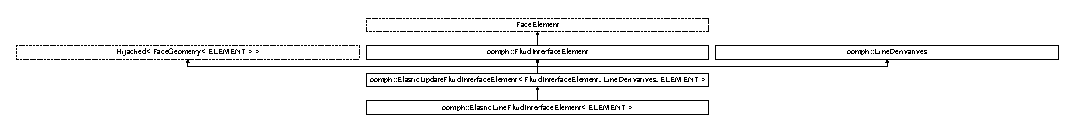
\includegraphics[height=1.307647cm]{classoomph_1_1ElasticLineFluidInterfaceElement}
\end{center}
\end{figure}
\subsection*{Public Member Functions}
\begin{DoxyCompactItemize}
\item 
\hyperlink{classoomph_1_1ElasticLineFluidInterfaceElement_ab0dde23477404e1c97956e40cfe361ab}{Elastic\+Line\+Fluid\+Interface\+Element} (Finite\+Element $\ast$const \&element\+\_\+pt, const int \&face\+\_\+index, const unsigned \&id=0)
\end{DoxyCompactItemize}
\subsection*{Additional Inherited Members}


\subsection{Detailed Description}
\subsubsection*{template$<$class E\+L\+E\+M\+E\+NT$>$\newline
class oomph\+::\+Elastic\+Line\+Fluid\+Interface\+Element$<$ E\+L\+E\+M\+E\+N\+T $>$}

Specialise the elastic update template class to concrete 1D case. 

Definition at line 1066 of file specific\+\_\+node\+\_\+update\+\_\+interface\+\_\+elements.\+h.



\subsection{Constructor \& Destructor Documentation}
\mbox{\Hypertarget{classoomph_1_1ElasticLineFluidInterfaceElement_ab0dde23477404e1c97956e40cfe361ab}\label{classoomph_1_1ElasticLineFluidInterfaceElement_ab0dde23477404e1c97956e40cfe361ab}} 
\index{oomph\+::\+Elastic\+Line\+Fluid\+Interface\+Element@{oomph\+::\+Elastic\+Line\+Fluid\+Interface\+Element}!Elastic\+Line\+Fluid\+Interface\+Element@{Elastic\+Line\+Fluid\+Interface\+Element}}
\index{Elastic\+Line\+Fluid\+Interface\+Element@{Elastic\+Line\+Fluid\+Interface\+Element}!oomph\+::\+Elastic\+Line\+Fluid\+Interface\+Element@{oomph\+::\+Elastic\+Line\+Fluid\+Interface\+Element}}
\subsubsection{\texorpdfstring{Elastic\+Line\+Fluid\+Interface\+Element()}{ElasticLineFluidInterfaceElement()}}
{\footnotesize\ttfamily template$<$class E\+L\+E\+M\+E\+NT $>$ \\
\hyperlink{classoomph_1_1ElasticLineFluidInterfaceElement}{oomph\+::\+Elastic\+Line\+Fluid\+Interface\+Element}$<$ E\+L\+E\+M\+E\+NT $>$\+::\hyperlink{classoomph_1_1ElasticLineFluidInterfaceElement}{Elastic\+Line\+Fluid\+Interface\+Element} (\begin{DoxyParamCaption}\item[{Finite\+Element $\ast$const \&}]{element\+\_\+pt,  }\item[{const int \&}]{face\+\_\+index,  }\item[{const unsigned \&}]{id = {\ttfamily 0} }\end{DoxyParamCaption})\hspace{0.3cm}{\ttfamily [inline]}}



Definition at line 1072 of file specific\+\_\+node\+\_\+update\+\_\+interface\+\_\+elements.\+h.



The documentation for this class was generated from the following file\+:\begin{DoxyCompactItemize}
\item 
\hyperlink{specific__node__update__interface__elements_8h}{specific\+\_\+node\+\_\+update\+\_\+interface\+\_\+elements.\+h}\end{DoxyCompactItemize}

\hypertarget{classoomph_1_1ElasticLineVolumeConstraintBoundingElement}{}\section{oomph\+:\+:Elastic\+Line\+Volume\+Constraint\+Bounding\+Element$<$ E\+L\+E\+M\+E\+NT $>$ Class Template Reference}
\label{classoomph_1_1ElasticLineVolumeConstraintBoundingElement}\index{oomph\+::\+Elastic\+Line\+Volume\+Constraint\+Bounding\+Element$<$ E\+L\+E\+M\+E\+N\+T $>$@{oomph\+::\+Elastic\+Line\+Volume\+Constraint\+Bounding\+Element$<$ E\+L\+E\+M\+E\+N\+T $>$}}


{\ttfamily \#include $<$constrained\+\_\+volume\+\_\+elements.\+h$>$}

Inheritance diagram for oomph\+:\+:Elastic\+Line\+Volume\+Constraint\+Bounding\+Element$<$ E\+L\+E\+M\+E\+NT $>$\+:\begin{figure}[H]
\begin{center}
\leavevmode
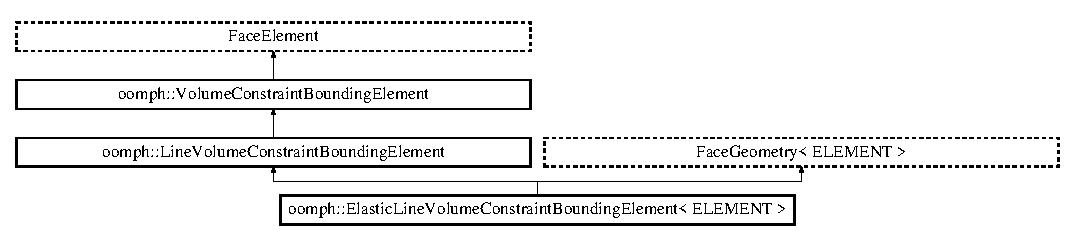
\includegraphics[height=2.786070cm]{classoomph_1_1ElasticLineVolumeConstraintBoundingElement}
\end{center}
\end{figure}
\subsection*{Public Member Functions}
\begin{DoxyCompactItemize}
\item 
\hyperlink{classoomph_1_1ElasticLineVolumeConstraintBoundingElement_a4759433aaab9f854126480581e4f08d5}{Elastic\+Line\+Volume\+Constraint\+Bounding\+Element} (\hyperlink{classoomph_1_1FiniteElement}{Finite\+Element} $\ast$const \&element\+\_\+pt, const int \&\hyperlink{classoomph_1_1FaceElement_a478d577ac6db67ecc80f1f02ae3ab170}{face\+\_\+index})
\begin{DoxyCompactList}\small\item\em Contructor\+: Specify bulk element and index of face to which this face element is to be attached. \end{DoxyCompactList}\item 
void \hyperlink{classoomph_1_1ElasticLineVolumeConstraintBoundingElement_a6b9670b4a995765e0b2793a3cab05966}{fill\+\_\+in\+\_\+contribution\+\_\+to\+\_\+jacobian} (\hyperlink{classoomph_1_1Vector}{Vector}$<$ double $>$ \&residuals, \hyperlink{classoomph_1_1DenseMatrix}{Dense\+Matrix}$<$ double $>$ \&jacobian)
\item 
double \hyperlink{classoomph_1_1ElasticLineVolumeConstraintBoundingElement_a99fee8b9d2bea757909174f26415139b}{zeta\+\_\+nodal} (const unsigned \&n, const unsigned \&k, const unsigned \&\hyperlink{cfortran_8h_adb50e893b86b3e55e751a42eab3cba82}{i}) const
\begin{DoxyCompactList}\small\item\em The \char`\"{}global\char`\"{} intrinsic coordinate of the element when viewed as part of a geometric object should be given by the \hyperlink{classoomph_1_1FaceElement}{Face\+Element} representation, by default. \end{DoxyCompactList}\end{DoxyCompactItemize}
\subsection*{Additional Inherited Members}


\subsection{Detailed Description}
\subsubsection*{template$<$class E\+L\+E\+M\+E\+NT$>$\newline
class oomph\+::\+Elastic\+Line\+Volume\+Constraint\+Bounding\+Element$<$ E\+L\+E\+M\+E\+N\+T $>$}

The one-\/dimensional interface elements that allow imposition of a volume constraint specialised for the case when the nodal positions of the bulk elements are treated as solid degrees of freedom. To enforce that a fluid volume has a certain volume, attach these elements to all faces of the (2D cartesian) bulk fluid elements (of type E\+L\+E\+M\+E\+NT) that bound that region and then specify the \char`\"{}pressure\char`\"{} value that is traded for the constraint. 

Definition at line 381 of file constrained\+\_\+volume\+\_\+elements.\+h.



\subsection{Constructor \& Destructor Documentation}
\mbox{\Hypertarget{classoomph_1_1ElasticLineVolumeConstraintBoundingElement_a4759433aaab9f854126480581e4f08d5}\label{classoomph_1_1ElasticLineVolumeConstraintBoundingElement_a4759433aaab9f854126480581e4f08d5}} 
\index{oomph\+::\+Elastic\+Line\+Volume\+Constraint\+Bounding\+Element@{oomph\+::\+Elastic\+Line\+Volume\+Constraint\+Bounding\+Element}!Elastic\+Line\+Volume\+Constraint\+Bounding\+Element@{Elastic\+Line\+Volume\+Constraint\+Bounding\+Element}}
\index{Elastic\+Line\+Volume\+Constraint\+Bounding\+Element@{Elastic\+Line\+Volume\+Constraint\+Bounding\+Element}!oomph\+::\+Elastic\+Line\+Volume\+Constraint\+Bounding\+Element@{oomph\+::\+Elastic\+Line\+Volume\+Constraint\+Bounding\+Element}}
\subsubsection{\texorpdfstring{Elastic\+Line\+Volume\+Constraint\+Bounding\+Element()}{ElasticLineVolumeConstraintBoundingElement()}}
{\footnotesize\ttfamily template$<$class E\+L\+E\+M\+E\+NT $>$ \\
\hyperlink{classoomph_1_1ElasticLineVolumeConstraintBoundingElement}{oomph\+::\+Elastic\+Line\+Volume\+Constraint\+Bounding\+Element}$<$ E\+L\+E\+M\+E\+NT $>$\+::\hyperlink{classoomph_1_1ElasticLineVolumeConstraintBoundingElement}{Elastic\+Line\+Volume\+Constraint\+Bounding\+Element} (\begin{DoxyParamCaption}\item[{\hyperlink{classoomph_1_1FiniteElement}{Finite\+Element} $\ast$const \&}]{element\+\_\+pt,  }\item[{const int \&}]{face\+\_\+index }\end{DoxyParamCaption})\hspace{0.3cm}{\ttfamily [inline]}}



Contructor\+: Specify bulk element and index of face to which this face element is to be attached. 



Definition at line 390 of file constrained\+\_\+volume\+\_\+elements.\+h.



References oomph\+::\+Finite\+Element\+::build\+\_\+face\+\_\+element().



\subsection{Member Function Documentation}
\mbox{\Hypertarget{classoomph_1_1ElasticLineVolumeConstraintBoundingElement_a6b9670b4a995765e0b2793a3cab05966}\label{classoomph_1_1ElasticLineVolumeConstraintBoundingElement_a6b9670b4a995765e0b2793a3cab05966}} 
\index{oomph\+::\+Elastic\+Line\+Volume\+Constraint\+Bounding\+Element@{oomph\+::\+Elastic\+Line\+Volume\+Constraint\+Bounding\+Element}!fill\+\_\+in\+\_\+contribution\+\_\+to\+\_\+jacobian@{fill\+\_\+in\+\_\+contribution\+\_\+to\+\_\+jacobian}}
\index{fill\+\_\+in\+\_\+contribution\+\_\+to\+\_\+jacobian@{fill\+\_\+in\+\_\+contribution\+\_\+to\+\_\+jacobian}!oomph\+::\+Elastic\+Line\+Volume\+Constraint\+Bounding\+Element@{oomph\+::\+Elastic\+Line\+Volume\+Constraint\+Bounding\+Element}}
\subsubsection{\texorpdfstring{fill\+\_\+in\+\_\+contribution\+\_\+to\+\_\+jacobian()}{fill\_in\_contribution\_to\_jacobian()}}
{\footnotesize\ttfamily template$<$class E\+L\+E\+M\+E\+NT $>$ \\
void \hyperlink{classoomph_1_1ElasticLineVolumeConstraintBoundingElement}{oomph\+::\+Elastic\+Line\+Volume\+Constraint\+Bounding\+Element}$<$ E\+L\+E\+M\+E\+NT $>$\+::fill\+\_\+in\+\_\+contribution\+\_\+to\+\_\+jacobian (\begin{DoxyParamCaption}\item[{\hyperlink{classoomph_1_1Vector}{Vector}$<$ double $>$ \&}]{residuals,  }\item[{\hyperlink{classoomph_1_1DenseMatrix}{Dense\+Matrix}$<$ double $>$ \&}]{jacobian }\end{DoxyParamCaption})\hspace{0.3cm}{\ttfamily [inline]}, {\ttfamily [virtual]}}

Fill in contribution to residuals and Jacobian. This is specific to solid-\/based elements in which derivatives w.\+r.\+t. to nodal positions are evaluated by finite differencing 

Reimplemented from \hyperlink{classoomph_1_1GeneralisedElement_a6ae09fc0d68e4309ac1b03583d252845}{oomph\+::\+Generalised\+Element}.



Definition at line 403 of file constrained\+\_\+volume\+\_\+elements.\+h.

\mbox{\Hypertarget{classoomph_1_1ElasticLineVolumeConstraintBoundingElement_a99fee8b9d2bea757909174f26415139b}\label{classoomph_1_1ElasticLineVolumeConstraintBoundingElement_a99fee8b9d2bea757909174f26415139b}} 
\index{oomph\+::\+Elastic\+Line\+Volume\+Constraint\+Bounding\+Element@{oomph\+::\+Elastic\+Line\+Volume\+Constraint\+Bounding\+Element}!zeta\+\_\+nodal@{zeta\+\_\+nodal}}
\index{zeta\+\_\+nodal@{zeta\+\_\+nodal}!oomph\+::\+Elastic\+Line\+Volume\+Constraint\+Bounding\+Element@{oomph\+::\+Elastic\+Line\+Volume\+Constraint\+Bounding\+Element}}
\subsubsection{\texorpdfstring{zeta\+\_\+nodal()}{zeta\_nodal()}}
{\footnotesize\ttfamily template$<$class E\+L\+E\+M\+E\+NT $>$ \\
double \hyperlink{classoomph_1_1ElasticLineVolumeConstraintBoundingElement}{oomph\+::\+Elastic\+Line\+Volume\+Constraint\+Bounding\+Element}$<$ E\+L\+E\+M\+E\+NT $>$\+::zeta\+\_\+nodal (\begin{DoxyParamCaption}\item[{const unsigned \&}]{n,  }\item[{const unsigned \&}]{k,  }\item[{const unsigned \&}]{i }\end{DoxyParamCaption}) const\hspace{0.3cm}{\ttfamily [inline]}, {\ttfamily [virtual]}}



The \char`\"{}global\char`\"{} intrinsic coordinate of the element when viewed as part of a geometric object should be given by the \hyperlink{classoomph_1_1FaceElement}{Face\+Element} representation, by default. 



Reimplemented from \hyperlink{classoomph_1_1FiniteElement_a849561c5fbcbc07dc49d2dc6cca68559}{oomph\+::\+Finite\+Element}.



Definition at line 417 of file constrained\+\_\+volume\+\_\+elements.\+h.



References oomph\+::\+Face\+Element\+::zeta\+\_\+nodal().



The documentation for this class was generated from the following file\+:\begin{DoxyCompactItemize}
\item 
\hyperlink{constrained__volume__elements_8h}{constrained\+\_\+volume\+\_\+elements.\+h}\end{DoxyCompactItemize}

\hypertarget{classoomph_1_1ElasticPointFluidInterfaceBoundingElement}{}\section{oomph\+:\+:Elastic\+Point\+Fluid\+Interface\+Bounding\+Element$<$ E\+L\+E\+M\+E\+NT $>$ Class Template Reference}
\label{classoomph_1_1ElasticPointFluidInterfaceBoundingElement}\index{oomph\+::\+Elastic\+Point\+Fluid\+Interface\+Bounding\+Element$<$ E\+L\+E\+M\+E\+N\+T $>$@{oomph\+::\+Elastic\+Point\+Fluid\+Interface\+Bounding\+Element$<$ E\+L\+E\+M\+E\+N\+T $>$}}


Pseudo-\/elasticity version of the \hyperlink{classoomph_1_1PointFluidInterfaceBoundingElement}{Point\+Fluid\+Interface\+Bounding\+Element}.  




{\ttfamily \#include $<$specific\+\_\+node\+\_\+update\+\_\+interface\+\_\+elements.\+h$>$}

Inheritance diagram for oomph\+:\+:Elastic\+Point\+Fluid\+Interface\+Bounding\+Element$<$ E\+L\+E\+M\+E\+NT $>$\+:\begin{figure}[H]
\begin{center}
\leavevmode
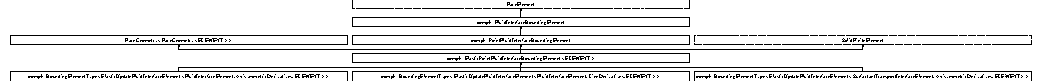
\includegraphics[height=1.147541cm]{classoomph_1_1ElasticPointFluidInterfaceBoundingElement}
\end{center}
\end{figure}
\subsection*{Public Member Functions}
\begin{DoxyCompactItemize}
\item 
void \hyperlink{classoomph_1_1ElasticPointFluidInterfaceBoundingElement_a9a36ac6e616ed271507cbfe26de085b4}{set\+\_\+lagrange\+\_\+index} (const \hyperlink{classoomph_1_1Vector}{Vector}$<$ unsigned $>$ \&lagrange\+\_\+index)
\begin{DoxyCompactList}\small\item\em Set the Id and offset. \end{DoxyCompactList}\item 
double \hyperlink{classoomph_1_1ElasticPointFluidInterfaceBoundingElement_a9d72fee284b866769347fb471c5828ad}{zeta\+\_\+nodal} (const unsigned \&n, const unsigned \&k, const unsigned \&\hyperlink{cfortran_8h_adb50e893b86b3e55e751a42eab3cba82}{i}) const
\begin{DoxyCompactList}\small\item\em Specify the value of nodal zeta from the face geometry The \char`\"{}global\char`\"{} intrinsic coordinate of the element when viewed as part of a geometric object should be given by the \hyperlink{classoomph_1_1FaceElement}{Face\+Element} representation, by default. \end{DoxyCompactList}\item 
\hyperlink{classoomph_1_1ElasticPointFluidInterfaceBoundingElement_a18e40e63a31953ad02cb0a2e7d0577b3}{Elastic\+Point\+Fluid\+Interface\+Bounding\+Element} ()
\begin{DoxyCompactList}\small\item\em Constructor. \end{DoxyCompactList}\item 
void \hyperlink{classoomph_1_1ElasticPointFluidInterfaceBoundingElement_a3a09e94ba3bf5ce0922bc4b75097078c}{output} (std\+::ostream \&outfile)
\begin{DoxyCompactList}\small\item\em Overload the output function. \end{DoxyCompactList}\item 
void \hyperlink{classoomph_1_1ElasticPointFluidInterfaceBoundingElement_a20c0678a9fdd6ef91fe48aa1b9209c38}{output} (std\+::ostream \&outfile, const unsigned \&n\+\_\+plot)
\begin{DoxyCompactList}\small\item\em Output the element. \end{DoxyCompactList}\item 
void \hyperlink{classoomph_1_1ElasticPointFluidInterfaceBoundingElement_a61782633205934c9af1aead51640e220}{output} (F\+I\+LE $\ast$file\+\_\+pt)
\begin{DoxyCompactList}\small\item\em Overload the C-\/style output function. \end{DoxyCompactList}\item 
void \hyperlink{classoomph_1_1ElasticPointFluidInterfaceBoundingElement_a4b30d56cc1869b5c9c4819843fb65ecc}{output} (F\+I\+LE $\ast$file\+\_\+pt, const unsigned \&n\+\_\+plot)
\begin{DoxyCompactList}\small\item\em C-\/style Output function. \end{DoxyCompactList}\item 
void \hyperlink{classoomph_1_1ElasticPointFluidInterfaceBoundingElement_a87802dab899430374a926d1e1bf3d90b}{fill\+\_\+in\+\_\+contribution\+\_\+to\+\_\+jacobian} (\hyperlink{classoomph_1_1Vector}{Vector}$<$ double $>$ \&residuals, \hyperlink{classoomph_1_1DenseMatrix}{Dense\+Matrix}$<$ double $>$ \&jacobian)
\begin{DoxyCompactList}\small\item\em Calculate the element\textquotesingle{}s residual vector and Jacobian. \end{DoxyCompactList}\item 
int \hyperlink{classoomph_1_1ElasticPointFluidInterfaceBoundingElement_ac3d7ce3db705bee219bf56cbb0d9ba92}{kinematic\+\_\+local\+\_\+eqn} (const unsigned \&n)
\begin{DoxyCompactList}\small\item\em Set the kinematic local equation. \end{DoxyCompactList}\end{DoxyCompactItemize}
\subsection*{Private Attributes}
\begin{DoxyCompactItemize}
\item 
\hyperlink{classoomph_1_1Vector}{Vector}$<$ unsigned $>$ \hyperlink{classoomph_1_1ElasticPointFluidInterfaceBoundingElement_a6ba345f9959aa12708c3ef8598327bc2}{Lagrange\+\_\+index}
\begin{DoxyCompactList}\small\item\em Short Storage for the index of the Lagrange multiplier at the chosen nodes. \end{DoxyCompactList}\end{DoxyCompactItemize}
\subsection*{Additional Inherited Members}


\subsection{Detailed Description}
\subsubsection*{template$<$class E\+L\+E\+M\+E\+NT$>$\newline
class oomph\+::\+Elastic\+Point\+Fluid\+Interface\+Bounding\+Element$<$ E\+L\+E\+M\+E\+N\+T $>$}

Pseudo-\/elasticity version of the \hyperlink{classoomph_1_1PointFluidInterfaceBoundingElement}{Point\+Fluid\+Interface\+Bounding\+Element}. 

Definition at line 919 of file specific\+\_\+node\+\_\+update\+\_\+interface\+\_\+elements.\+h.



\subsection{Constructor \& Destructor Documentation}
\mbox{\Hypertarget{classoomph_1_1ElasticPointFluidInterfaceBoundingElement_a18e40e63a31953ad02cb0a2e7d0577b3}\label{classoomph_1_1ElasticPointFluidInterfaceBoundingElement_a18e40e63a31953ad02cb0a2e7d0577b3}} 
\index{oomph\+::\+Elastic\+Point\+Fluid\+Interface\+Bounding\+Element@{oomph\+::\+Elastic\+Point\+Fluid\+Interface\+Bounding\+Element}!Elastic\+Point\+Fluid\+Interface\+Bounding\+Element@{Elastic\+Point\+Fluid\+Interface\+Bounding\+Element}}
\index{Elastic\+Point\+Fluid\+Interface\+Bounding\+Element@{Elastic\+Point\+Fluid\+Interface\+Bounding\+Element}!oomph\+::\+Elastic\+Point\+Fluid\+Interface\+Bounding\+Element@{oomph\+::\+Elastic\+Point\+Fluid\+Interface\+Bounding\+Element}}
\subsubsection{\texorpdfstring{Elastic\+Point\+Fluid\+Interface\+Bounding\+Element()}{ElasticPointFluidInterfaceBoundingElement()}}
{\footnotesize\ttfamily template$<$class E\+L\+E\+M\+E\+NT $>$ \\
\hyperlink{classoomph_1_1ElasticPointFluidInterfaceBoundingElement}{oomph\+::\+Elastic\+Point\+Fluid\+Interface\+Bounding\+Element}$<$ E\+L\+E\+M\+E\+NT $>$\+::\hyperlink{classoomph_1_1ElasticPointFluidInterfaceBoundingElement}{Elastic\+Point\+Fluid\+Interface\+Bounding\+Element} (\begin{DoxyParamCaption}{ }\end{DoxyParamCaption})\hspace{0.3cm}{\ttfamily [inline]}}



Constructor. 



Definition at line 946 of file specific\+\_\+node\+\_\+update\+\_\+interface\+\_\+elements.\+h.



\subsection{Member Function Documentation}
\mbox{\Hypertarget{classoomph_1_1ElasticPointFluidInterfaceBoundingElement_a87802dab899430374a926d1e1bf3d90b}\label{classoomph_1_1ElasticPointFluidInterfaceBoundingElement_a87802dab899430374a926d1e1bf3d90b}} 
\index{oomph\+::\+Elastic\+Point\+Fluid\+Interface\+Bounding\+Element@{oomph\+::\+Elastic\+Point\+Fluid\+Interface\+Bounding\+Element}!fill\+\_\+in\+\_\+contribution\+\_\+to\+\_\+jacobian@{fill\+\_\+in\+\_\+contribution\+\_\+to\+\_\+jacobian}}
\index{fill\+\_\+in\+\_\+contribution\+\_\+to\+\_\+jacobian@{fill\+\_\+in\+\_\+contribution\+\_\+to\+\_\+jacobian}!oomph\+::\+Elastic\+Point\+Fluid\+Interface\+Bounding\+Element@{oomph\+::\+Elastic\+Point\+Fluid\+Interface\+Bounding\+Element}}
\subsubsection{\texorpdfstring{fill\+\_\+in\+\_\+contribution\+\_\+to\+\_\+jacobian()}{fill\_in\_contribution\_to\_jacobian()}}
{\footnotesize\ttfamily template$<$class E\+L\+E\+M\+E\+NT $>$ \\
void \hyperlink{classoomph_1_1ElasticPointFluidInterfaceBoundingElement}{oomph\+::\+Elastic\+Point\+Fluid\+Interface\+Bounding\+Element}$<$ E\+L\+E\+M\+E\+NT $>$\+::fill\+\_\+in\+\_\+contribution\+\_\+to\+\_\+jacobian (\begin{DoxyParamCaption}\item[{\hyperlink{classoomph_1_1Vector}{Vector}$<$ double $>$ \&}]{residuals,  }\item[{\hyperlink{classoomph_1_1DenseMatrix}{Dense\+Matrix}$<$ double $>$ \&}]{jacobian }\end{DoxyParamCaption})\hspace{0.3cm}{\ttfamily [inline]}, {\ttfamily [virtual]}}



Calculate the element\textquotesingle{}s residual vector and Jacobian. 



Reimplemented from \hyperlink{classoomph_1_1GeneralisedElement_a6ae09fc0d68e4309ac1b03583d252845}{oomph\+::\+Generalised\+Element}.



Definition at line 965 of file specific\+\_\+node\+\_\+update\+\_\+interface\+\_\+elements.\+h.

\mbox{\Hypertarget{classoomph_1_1ElasticPointFluidInterfaceBoundingElement_ac3d7ce3db705bee219bf56cbb0d9ba92}\label{classoomph_1_1ElasticPointFluidInterfaceBoundingElement_ac3d7ce3db705bee219bf56cbb0d9ba92}} 
\index{oomph\+::\+Elastic\+Point\+Fluid\+Interface\+Bounding\+Element@{oomph\+::\+Elastic\+Point\+Fluid\+Interface\+Bounding\+Element}!kinematic\+\_\+local\+\_\+eqn@{kinematic\+\_\+local\+\_\+eqn}}
\index{kinematic\+\_\+local\+\_\+eqn@{kinematic\+\_\+local\+\_\+eqn}!oomph\+::\+Elastic\+Point\+Fluid\+Interface\+Bounding\+Element@{oomph\+::\+Elastic\+Point\+Fluid\+Interface\+Bounding\+Element}}
\subsubsection{\texorpdfstring{kinematic\+\_\+local\+\_\+eqn()}{kinematic\_local\_eqn()}}
{\footnotesize\ttfamily template$<$class E\+L\+E\+M\+E\+NT $>$ \\
int \hyperlink{classoomph_1_1ElasticPointFluidInterfaceBoundingElement}{oomph\+::\+Elastic\+Point\+Fluid\+Interface\+Bounding\+Element}$<$ E\+L\+E\+M\+E\+NT $>$\+::kinematic\+\_\+local\+\_\+eqn (\begin{DoxyParamCaption}\item[{const unsigned \&}]{n }\end{DoxyParamCaption})\hspace{0.3cm}{\ttfamily [inline]}, {\ttfamily [virtual]}}



Set the kinematic local equation. 



Implements \hyperlink{classoomph_1_1FluidInterfaceBoundingElement_a12a0a6d7c3c1c1a5a0f42a57e60eab34}{oomph\+::\+Fluid\+Interface\+Bounding\+Element}.



Definition at line 979 of file specific\+\_\+node\+\_\+update\+\_\+interface\+\_\+elements.\+h.

\mbox{\Hypertarget{classoomph_1_1ElasticPointFluidInterfaceBoundingElement_a3a09e94ba3bf5ce0922bc4b75097078c}\label{classoomph_1_1ElasticPointFluidInterfaceBoundingElement_a3a09e94ba3bf5ce0922bc4b75097078c}} 
\index{oomph\+::\+Elastic\+Point\+Fluid\+Interface\+Bounding\+Element@{oomph\+::\+Elastic\+Point\+Fluid\+Interface\+Bounding\+Element}!output@{output}}
\index{output@{output}!oomph\+::\+Elastic\+Point\+Fluid\+Interface\+Bounding\+Element@{oomph\+::\+Elastic\+Point\+Fluid\+Interface\+Bounding\+Element}}
\subsubsection{\texorpdfstring{output()}{output()}\hspace{0.1cm}{\footnotesize\ttfamily [1/4]}}
{\footnotesize\ttfamily template$<$class E\+L\+E\+M\+E\+NT $>$ \\
void \hyperlink{classoomph_1_1ElasticPointFluidInterfaceBoundingElement}{oomph\+::\+Elastic\+Point\+Fluid\+Interface\+Bounding\+Element}$<$ E\+L\+E\+M\+E\+NT $>$\+::output (\begin{DoxyParamCaption}\item[{std\+::ostream \&}]{outfile }\end{DoxyParamCaption})\hspace{0.3cm}{\ttfamily [inline]}, {\ttfamily [virtual]}}



Overload the output function. 



Reimplemented from \hyperlink{classoomph_1_1FluidInterfaceBoundingElement_a81adc5ae89ddfa120f587c61b972622f}{oomph\+::\+Fluid\+Interface\+Bounding\+Element}.



Definition at line 951 of file specific\+\_\+node\+\_\+update\+\_\+interface\+\_\+elements.\+h.



References oomph\+::\+Finite\+Element\+::output().

\mbox{\Hypertarget{classoomph_1_1ElasticPointFluidInterfaceBoundingElement_a20c0678a9fdd6ef91fe48aa1b9209c38}\label{classoomph_1_1ElasticPointFluidInterfaceBoundingElement_a20c0678a9fdd6ef91fe48aa1b9209c38}} 
\index{oomph\+::\+Elastic\+Point\+Fluid\+Interface\+Bounding\+Element@{oomph\+::\+Elastic\+Point\+Fluid\+Interface\+Bounding\+Element}!output@{output}}
\index{output@{output}!oomph\+::\+Elastic\+Point\+Fluid\+Interface\+Bounding\+Element@{oomph\+::\+Elastic\+Point\+Fluid\+Interface\+Bounding\+Element}}
\subsubsection{\texorpdfstring{output()}{output()}\hspace{0.1cm}{\footnotesize\ttfamily [2/4]}}
{\footnotesize\ttfamily template$<$class E\+L\+E\+M\+E\+NT $>$ \\
void \hyperlink{classoomph_1_1ElasticPointFluidInterfaceBoundingElement}{oomph\+::\+Elastic\+Point\+Fluid\+Interface\+Bounding\+Element}$<$ E\+L\+E\+M\+E\+NT $>$\+::output (\begin{DoxyParamCaption}\item[{std\+::ostream \&}]{outfile,  }\item[{const unsigned \&}]{n\+\_\+plot }\end{DoxyParamCaption})\hspace{0.3cm}{\ttfamily [inline]}, {\ttfamily [virtual]}}



Output the element. 



Reimplemented from \hyperlink{classoomph_1_1FluidInterfaceBoundingElement_af2c821d51d506221976a0c17e1615ac3}{oomph\+::\+Fluid\+Interface\+Bounding\+Element}.



Definition at line 954 of file specific\+\_\+node\+\_\+update\+\_\+interface\+\_\+elements.\+h.



References oomph\+::\+Fluid\+Interface\+Bounding\+Element\+::output().

\mbox{\Hypertarget{classoomph_1_1ElasticPointFluidInterfaceBoundingElement_a61782633205934c9af1aead51640e220}\label{classoomph_1_1ElasticPointFluidInterfaceBoundingElement_a61782633205934c9af1aead51640e220}} 
\index{oomph\+::\+Elastic\+Point\+Fluid\+Interface\+Bounding\+Element@{oomph\+::\+Elastic\+Point\+Fluid\+Interface\+Bounding\+Element}!output@{output}}
\index{output@{output}!oomph\+::\+Elastic\+Point\+Fluid\+Interface\+Bounding\+Element@{oomph\+::\+Elastic\+Point\+Fluid\+Interface\+Bounding\+Element}}
\subsubsection{\texorpdfstring{output()}{output()}\hspace{0.1cm}{\footnotesize\ttfamily [3/4]}}
{\footnotesize\ttfamily template$<$class E\+L\+E\+M\+E\+NT $>$ \\
void \hyperlink{classoomph_1_1ElasticPointFluidInterfaceBoundingElement}{oomph\+::\+Elastic\+Point\+Fluid\+Interface\+Bounding\+Element}$<$ E\+L\+E\+M\+E\+NT $>$\+::output (\begin{DoxyParamCaption}\item[{F\+I\+LE $\ast$}]{file\+\_\+pt }\end{DoxyParamCaption})\hspace{0.3cm}{\ttfamily [inline]}, {\ttfamily [virtual]}}



Overload the C-\/style output function. 



Reimplemented from \hyperlink{classoomph_1_1FluidInterfaceBoundingElement_a85cc62405429744e3e3585894315cb9e}{oomph\+::\+Fluid\+Interface\+Bounding\+Element}.



Definition at line 958 of file specific\+\_\+node\+\_\+update\+\_\+interface\+\_\+elements.\+h.



References oomph\+::\+Finite\+Element\+::output().

\mbox{\Hypertarget{classoomph_1_1ElasticPointFluidInterfaceBoundingElement_a4b30d56cc1869b5c9c4819843fb65ecc}\label{classoomph_1_1ElasticPointFluidInterfaceBoundingElement_a4b30d56cc1869b5c9c4819843fb65ecc}} 
\index{oomph\+::\+Elastic\+Point\+Fluid\+Interface\+Bounding\+Element@{oomph\+::\+Elastic\+Point\+Fluid\+Interface\+Bounding\+Element}!output@{output}}
\index{output@{output}!oomph\+::\+Elastic\+Point\+Fluid\+Interface\+Bounding\+Element@{oomph\+::\+Elastic\+Point\+Fluid\+Interface\+Bounding\+Element}}
\subsubsection{\texorpdfstring{output()}{output()}\hspace{0.1cm}{\footnotesize\ttfamily [4/4]}}
{\footnotesize\ttfamily template$<$class E\+L\+E\+M\+E\+NT $>$ \\
void \hyperlink{classoomph_1_1ElasticPointFluidInterfaceBoundingElement}{oomph\+::\+Elastic\+Point\+Fluid\+Interface\+Bounding\+Element}$<$ E\+L\+E\+M\+E\+NT $>$\+::output (\begin{DoxyParamCaption}\item[{F\+I\+LE $\ast$}]{file\+\_\+pt,  }\item[{const unsigned \&}]{n\+\_\+plot }\end{DoxyParamCaption})\hspace{0.3cm}{\ttfamily [inline]}, {\ttfamily [virtual]}}



C-\/style Output function. 



Reimplemented from \hyperlink{classoomph_1_1FluidInterfaceBoundingElement_ae85ea987a06275a03ad6d0e3710871da}{oomph\+::\+Fluid\+Interface\+Bounding\+Element}.



Definition at line 961 of file specific\+\_\+node\+\_\+update\+\_\+interface\+\_\+elements.\+h.



References oomph\+::\+Fluid\+Interface\+Bounding\+Element\+::output().

\mbox{\Hypertarget{classoomph_1_1ElasticPointFluidInterfaceBoundingElement_a9a36ac6e616ed271507cbfe26de085b4}\label{classoomph_1_1ElasticPointFluidInterfaceBoundingElement_a9a36ac6e616ed271507cbfe26de085b4}} 
\index{oomph\+::\+Elastic\+Point\+Fluid\+Interface\+Bounding\+Element@{oomph\+::\+Elastic\+Point\+Fluid\+Interface\+Bounding\+Element}!set\+\_\+lagrange\+\_\+index@{set\+\_\+lagrange\+\_\+index}}
\index{set\+\_\+lagrange\+\_\+index@{set\+\_\+lagrange\+\_\+index}!oomph\+::\+Elastic\+Point\+Fluid\+Interface\+Bounding\+Element@{oomph\+::\+Elastic\+Point\+Fluid\+Interface\+Bounding\+Element}}
\subsubsection{\texorpdfstring{set\+\_\+lagrange\+\_\+index()}{set\_lagrange\_index()}}
{\footnotesize\ttfamily template$<$class E\+L\+E\+M\+E\+NT $>$ \\
void \hyperlink{classoomph_1_1ElasticPointFluidInterfaceBoundingElement}{oomph\+::\+Elastic\+Point\+Fluid\+Interface\+Bounding\+Element}$<$ E\+L\+E\+M\+E\+NT $>$\+::set\+\_\+lagrange\+\_\+index (\begin{DoxyParamCaption}\item[{const \hyperlink{classoomph_1_1Vector}{Vector}$<$ unsigned $>$ \&}]{lagrange\+\_\+index }\end{DoxyParamCaption})\hspace{0.3cm}{\ttfamily [inline]}}



Set the Id and offset. 



Definition at line 932 of file specific\+\_\+node\+\_\+update\+\_\+interface\+\_\+elements.\+h.

\mbox{\Hypertarget{classoomph_1_1ElasticPointFluidInterfaceBoundingElement_a9d72fee284b866769347fb471c5828ad}\label{classoomph_1_1ElasticPointFluidInterfaceBoundingElement_a9d72fee284b866769347fb471c5828ad}} 
\index{oomph\+::\+Elastic\+Point\+Fluid\+Interface\+Bounding\+Element@{oomph\+::\+Elastic\+Point\+Fluid\+Interface\+Bounding\+Element}!zeta\+\_\+nodal@{zeta\+\_\+nodal}}
\index{zeta\+\_\+nodal@{zeta\+\_\+nodal}!oomph\+::\+Elastic\+Point\+Fluid\+Interface\+Bounding\+Element@{oomph\+::\+Elastic\+Point\+Fluid\+Interface\+Bounding\+Element}}
\subsubsection{\texorpdfstring{zeta\+\_\+nodal()}{zeta\_nodal()}}
{\footnotesize\ttfamily template$<$class E\+L\+E\+M\+E\+NT $>$ \\
double \hyperlink{classoomph_1_1ElasticPointFluidInterfaceBoundingElement}{oomph\+::\+Elastic\+Point\+Fluid\+Interface\+Bounding\+Element}$<$ E\+L\+E\+M\+E\+NT $>$\+::zeta\+\_\+nodal (\begin{DoxyParamCaption}\item[{const unsigned \&}]{n,  }\item[{const unsigned \&}]{k,  }\item[{const unsigned \&}]{i }\end{DoxyParamCaption}) const\hspace{0.3cm}{\ttfamily [inline]}, {\ttfamily [virtual]}}



Specify the value of nodal zeta from the face geometry The \char`\"{}global\char`\"{} intrinsic coordinate of the element when viewed as part of a geometric object should be given by the \hyperlink{classoomph_1_1FaceElement}{Face\+Element} representation, by default. 



Reimplemented from \hyperlink{classoomph_1_1FiniteElement_a849561c5fbcbc07dc49d2dc6cca68559}{oomph\+::\+Finite\+Element}.



Definition at line 940 of file specific\+\_\+node\+\_\+update\+\_\+interface\+\_\+elements.\+h.



References oomph\+::\+Face\+Element\+::zeta\+\_\+nodal().



\subsection{Member Data Documentation}
\mbox{\Hypertarget{classoomph_1_1ElasticPointFluidInterfaceBoundingElement_a6ba345f9959aa12708c3ef8598327bc2}\label{classoomph_1_1ElasticPointFluidInterfaceBoundingElement_a6ba345f9959aa12708c3ef8598327bc2}} 
\index{oomph\+::\+Elastic\+Point\+Fluid\+Interface\+Bounding\+Element@{oomph\+::\+Elastic\+Point\+Fluid\+Interface\+Bounding\+Element}!Lagrange\+\_\+index@{Lagrange\+\_\+index}}
\index{Lagrange\+\_\+index@{Lagrange\+\_\+index}!oomph\+::\+Elastic\+Point\+Fluid\+Interface\+Bounding\+Element@{oomph\+::\+Elastic\+Point\+Fluid\+Interface\+Bounding\+Element}}
\subsubsection{\texorpdfstring{Lagrange\+\_\+index}{Lagrange\_index}}
{\footnotesize\ttfamily template$<$class E\+L\+E\+M\+E\+NT $>$ \\
\hyperlink{classoomph_1_1Vector}{Vector}$<$unsigned$>$ \hyperlink{classoomph_1_1ElasticPointFluidInterfaceBoundingElement}{oomph\+::\+Elastic\+Point\+Fluid\+Interface\+Bounding\+Element}$<$ E\+L\+E\+M\+E\+NT $>$\+::Lagrange\+\_\+index\hspace{0.3cm}{\ttfamily [private]}}



Short Storage for the index of the Lagrange multiplier at the chosen nodes. 



Definition at line 927 of file specific\+\_\+node\+\_\+update\+\_\+interface\+\_\+elements.\+h.



The documentation for this class was generated from the following file\+:\begin{DoxyCompactItemize}
\item 
\hyperlink{specific__node__update__interface__elements_8h}{specific\+\_\+node\+\_\+update\+\_\+interface\+\_\+elements.\+h}\end{DoxyCompactItemize}

\hypertarget{classoomph_1_1ElasticSurfaceFluidInterfaceElement}{}\section{oomph\+:\+:Elastic\+Surface\+Fluid\+Interface\+Element$<$ E\+L\+E\+M\+E\+NT $>$ Class Template Reference}
\label{classoomph_1_1ElasticSurfaceFluidInterfaceElement}\index{oomph\+::\+Elastic\+Surface\+Fluid\+Interface\+Element$<$ E\+L\+E\+M\+E\+N\+T $>$@{oomph\+::\+Elastic\+Surface\+Fluid\+Interface\+Element$<$ E\+L\+E\+M\+E\+N\+T $>$}}


Specialise Elastic update case to the concrete 2D case.  




{\ttfamily \#include $<$specific\+\_\+node\+\_\+update\+\_\+interface\+\_\+elements.\+h$>$}

Inheritance diagram for oomph\+:\+:Elastic\+Surface\+Fluid\+Interface\+Element$<$ E\+L\+E\+M\+E\+NT $>$\+:\begin{figure}[H]
\begin{center}
\leavevmode
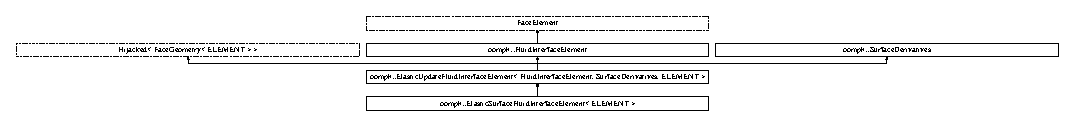
\includegraphics[height=1.418919cm]{classoomph_1_1ElasticSurfaceFluidInterfaceElement}
\end{center}
\end{figure}
\subsection*{Public Member Functions}
\begin{DoxyCompactItemize}
\item 
\hyperlink{classoomph_1_1ElasticSurfaceFluidInterfaceElement_aa2add34e23b16990c7000d699bc395e2}{Elastic\+Surface\+Fluid\+Interface\+Element} (\hyperlink{classoomph_1_1FiniteElement}{Finite\+Element} $\ast$const \&element\+\_\+pt, const int \&\hyperlink{classoomph_1_1FaceElement_a478d577ac6db67ecc80f1f02ae3ab170}{face\+\_\+index}, const unsigned \&id=0)
\end{DoxyCompactItemize}
\subsection*{Additional Inherited Members}


\subsection{Detailed Description}
\subsubsection*{template$<$class E\+L\+E\+M\+E\+NT$>$\newline
class oomph\+::\+Elastic\+Surface\+Fluid\+Interface\+Element$<$ E\+L\+E\+M\+E\+N\+T $>$}

Specialise Elastic update case to the concrete 2D case. 

Definition at line 1125 of file specific\+\_\+node\+\_\+update\+\_\+interface\+\_\+elements.\+h.



\subsection{Constructor \& Destructor Documentation}
\mbox{\Hypertarget{classoomph_1_1ElasticSurfaceFluidInterfaceElement_aa2add34e23b16990c7000d699bc395e2}\label{classoomph_1_1ElasticSurfaceFluidInterfaceElement_aa2add34e23b16990c7000d699bc395e2}} 
\index{oomph\+::\+Elastic\+Surface\+Fluid\+Interface\+Element@{oomph\+::\+Elastic\+Surface\+Fluid\+Interface\+Element}!Elastic\+Surface\+Fluid\+Interface\+Element@{Elastic\+Surface\+Fluid\+Interface\+Element}}
\index{Elastic\+Surface\+Fluid\+Interface\+Element@{Elastic\+Surface\+Fluid\+Interface\+Element}!oomph\+::\+Elastic\+Surface\+Fluid\+Interface\+Element@{oomph\+::\+Elastic\+Surface\+Fluid\+Interface\+Element}}
\subsubsection{\texorpdfstring{Elastic\+Surface\+Fluid\+Interface\+Element()}{ElasticSurfaceFluidInterfaceElement()}}
{\footnotesize\ttfamily template$<$class E\+L\+E\+M\+E\+NT $>$ \\
\hyperlink{classoomph_1_1ElasticSurfaceFluidInterfaceElement}{oomph\+::\+Elastic\+Surface\+Fluid\+Interface\+Element}$<$ E\+L\+E\+M\+E\+NT $>$\+::\hyperlink{classoomph_1_1ElasticSurfaceFluidInterfaceElement}{Elastic\+Surface\+Fluid\+Interface\+Element} (\begin{DoxyParamCaption}\item[{\hyperlink{classoomph_1_1FiniteElement}{Finite\+Element} $\ast$const \&}]{element\+\_\+pt,  }\item[{const int \&}]{face\+\_\+index,  }\item[{const unsigned \&}]{id = {\ttfamily 0} }\end{DoxyParamCaption})\hspace{0.3cm}{\ttfamily [inline]}}



Definition at line 1131 of file specific\+\_\+node\+\_\+update\+\_\+interface\+\_\+elements.\+h.



The documentation for this class was generated from the following file\+:\begin{DoxyCompactItemize}
\item 
\hyperlink{specific__node__update__interface__elements_8h}{specific\+\_\+node\+\_\+update\+\_\+interface\+\_\+elements.\+h}\end{DoxyCompactItemize}

\hypertarget{classoomph_1_1ElasticSurfaceVolumeConstraintBoundingElement}{}\section{oomph\+:\+:Elastic\+Surface\+Volume\+Constraint\+Bounding\+Element$<$ E\+L\+E\+M\+E\+NT $>$ Class Template Reference}
\label{classoomph_1_1ElasticSurfaceVolumeConstraintBoundingElement}\index{oomph\+::\+Elastic\+Surface\+Volume\+Constraint\+Bounding\+Element$<$ E\+L\+E\+M\+E\+N\+T $>$@{oomph\+::\+Elastic\+Surface\+Volume\+Constraint\+Bounding\+Element$<$ E\+L\+E\+M\+E\+N\+T $>$}}


{\ttfamily \#include $<$constrained\+\_\+volume\+\_\+elements.\+h$>$}

Inheritance diagram for oomph\+:\+:Elastic\+Surface\+Volume\+Constraint\+Bounding\+Element$<$ E\+L\+E\+M\+E\+NT $>$\+:\begin{figure}[H]
\begin{center}
\leavevmode
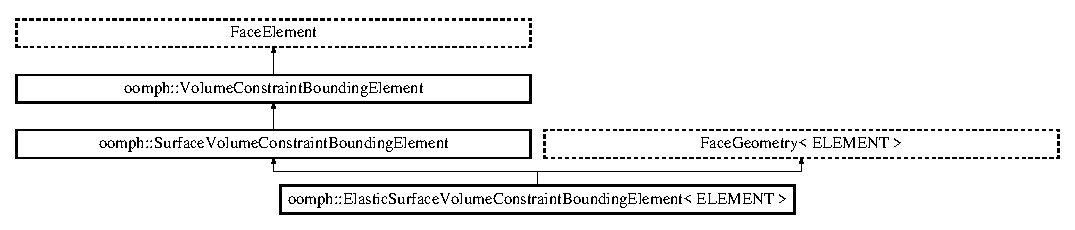
\includegraphics[height=2.647754cm]{classoomph_1_1ElasticSurfaceVolumeConstraintBoundingElement}
\end{center}
\end{figure}
\subsection*{Public Member Functions}
\begin{DoxyCompactItemize}
\item 
\hyperlink{classoomph_1_1ElasticSurfaceVolumeConstraintBoundingElement_a22e5cb7f3cb0d363301ae8ef232dd6cb}{Elastic\+Surface\+Volume\+Constraint\+Bounding\+Element} (Finite\+Element $\ast$const \&element\+\_\+pt, const int \&face\+\_\+index)
\begin{DoxyCompactList}\small\item\em Contructor\+: Specify bulk element and index of face to which this face element is to be attached. \end{DoxyCompactList}\item 
void \hyperlink{classoomph_1_1ElasticSurfaceVolumeConstraintBoundingElement_a16addc228d9871f22cd9eaf9b581ff5c}{fill\+\_\+in\+\_\+contribution\+\_\+to\+\_\+jacobian} (Vector$<$ double $>$ \&residuals, Dense\+Matrix$<$ double $>$ \&jacobian)
\item 
double \hyperlink{classoomph_1_1ElasticSurfaceVolumeConstraintBoundingElement_ab9826b68e1931ed4eafdf20af0bf070d}{zeta\+\_\+nodal} (const unsigned \&n, const unsigned \&k, const unsigned \&i) const
\begin{DoxyCompactList}\small\item\em The \char`\"{}global\char`\"{} intrinsic coordinate of the element when viewed as part of a geometric object should be given by the Face\+Element representation, by default. \end{DoxyCompactList}\end{DoxyCompactItemize}
\subsection*{Additional Inherited Members}


\subsection{Detailed Description}
\subsubsection*{template$<$class E\+L\+E\+M\+E\+NT$>$\newline
class oomph\+::\+Elastic\+Surface\+Volume\+Constraint\+Bounding\+Element$<$ E\+L\+E\+M\+E\+N\+T $>$}

The Two-\/dimensional interface elements that allow the application of a volume constraint specialised for the case when the nodal positions of the bulk elements are treated as solid degrees of freedom. To enforce that a fluid volume has a certain volume, attach these elements to all faces of the (3D Cartesian) bulk fluid elements (of type E\+L\+E\+M\+E\+NT) that bound that region and then specify the \char`\"{}pressure\char`\"{} value that is traded for the constraint. 

Definition at line 768 of file constrained\+\_\+volume\+\_\+elements.\+h.



\subsection{Constructor \& Destructor Documentation}
\mbox{\Hypertarget{classoomph_1_1ElasticSurfaceVolumeConstraintBoundingElement_a22e5cb7f3cb0d363301ae8ef232dd6cb}\label{classoomph_1_1ElasticSurfaceVolumeConstraintBoundingElement_a22e5cb7f3cb0d363301ae8ef232dd6cb}} 
\index{oomph\+::\+Elastic\+Surface\+Volume\+Constraint\+Bounding\+Element@{oomph\+::\+Elastic\+Surface\+Volume\+Constraint\+Bounding\+Element}!Elastic\+Surface\+Volume\+Constraint\+Bounding\+Element@{Elastic\+Surface\+Volume\+Constraint\+Bounding\+Element}}
\index{Elastic\+Surface\+Volume\+Constraint\+Bounding\+Element@{Elastic\+Surface\+Volume\+Constraint\+Bounding\+Element}!oomph\+::\+Elastic\+Surface\+Volume\+Constraint\+Bounding\+Element@{oomph\+::\+Elastic\+Surface\+Volume\+Constraint\+Bounding\+Element}}
\subsubsection{\texorpdfstring{Elastic\+Surface\+Volume\+Constraint\+Bounding\+Element()}{ElasticSurfaceVolumeConstraintBoundingElement()}}
{\footnotesize\ttfamily template$<$class E\+L\+E\+M\+E\+NT $>$ \\
\hyperlink{classoomph_1_1ElasticSurfaceVolumeConstraintBoundingElement}{oomph\+::\+Elastic\+Surface\+Volume\+Constraint\+Bounding\+Element}$<$ E\+L\+E\+M\+E\+NT $>$\+::\hyperlink{classoomph_1_1ElasticSurfaceVolumeConstraintBoundingElement}{Elastic\+Surface\+Volume\+Constraint\+Bounding\+Element} (\begin{DoxyParamCaption}\item[{Finite\+Element $\ast$const \&}]{element\+\_\+pt,  }\item[{const int \&}]{face\+\_\+index }\end{DoxyParamCaption})\hspace{0.3cm}{\ttfamily [inline]}}



Contructor\+: Specify bulk element and index of face to which this face element is to be attached. 



Definition at line 777 of file constrained\+\_\+volume\+\_\+elements.\+h.



\subsection{Member Function Documentation}
\mbox{\Hypertarget{classoomph_1_1ElasticSurfaceVolumeConstraintBoundingElement_a16addc228d9871f22cd9eaf9b581ff5c}\label{classoomph_1_1ElasticSurfaceVolumeConstraintBoundingElement_a16addc228d9871f22cd9eaf9b581ff5c}} 
\index{oomph\+::\+Elastic\+Surface\+Volume\+Constraint\+Bounding\+Element@{oomph\+::\+Elastic\+Surface\+Volume\+Constraint\+Bounding\+Element}!fill\+\_\+in\+\_\+contribution\+\_\+to\+\_\+jacobian@{fill\+\_\+in\+\_\+contribution\+\_\+to\+\_\+jacobian}}
\index{fill\+\_\+in\+\_\+contribution\+\_\+to\+\_\+jacobian@{fill\+\_\+in\+\_\+contribution\+\_\+to\+\_\+jacobian}!oomph\+::\+Elastic\+Surface\+Volume\+Constraint\+Bounding\+Element@{oomph\+::\+Elastic\+Surface\+Volume\+Constraint\+Bounding\+Element}}
\subsubsection{\texorpdfstring{fill\+\_\+in\+\_\+contribution\+\_\+to\+\_\+jacobian()}{fill\_in\_contribution\_to\_jacobian()}}
{\footnotesize\ttfamily template$<$class E\+L\+E\+M\+E\+NT $>$ \\
void \hyperlink{classoomph_1_1ElasticSurfaceVolumeConstraintBoundingElement}{oomph\+::\+Elastic\+Surface\+Volume\+Constraint\+Bounding\+Element}$<$ E\+L\+E\+M\+E\+NT $>$\+::fill\+\_\+in\+\_\+contribution\+\_\+to\+\_\+jacobian (\begin{DoxyParamCaption}\item[{Vector$<$ double $>$ \&}]{residuals,  }\item[{Dense\+Matrix$<$ double $>$ \&}]{jacobian }\end{DoxyParamCaption})\hspace{0.3cm}{\ttfamily [inline]}}

Fill in contribution to residuals and Jacobian. This is specific to solid-\/based elements in which derivatives w.\+r.\+t. to nodal positions are evaluated by finite differencing 

Definition at line 792 of file constrained\+\_\+volume\+\_\+elements.\+h.

\mbox{\Hypertarget{classoomph_1_1ElasticSurfaceVolumeConstraintBoundingElement_ab9826b68e1931ed4eafdf20af0bf070d}\label{classoomph_1_1ElasticSurfaceVolumeConstraintBoundingElement_ab9826b68e1931ed4eafdf20af0bf070d}} 
\index{oomph\+::\+Elastic\+Surface\+Volume\+Constraint\+Bounding\+Element@{oomph\+::\+Elastic\+Surface\+Volume\+Constraint\+Bounding\+Element}!zeta\+\_\+nodal@{zeta\+\_\+nodal}}
\index{zeta\+\_\+nodal@{zeta\+\_\+nodal}!oomph\+::\+Elastic\+Surface\+Volume\+Constraint\+Bounding\+Element@{oomph\+::\+Elastic\+Surface\+Volume\+Constraint\+Bounding\+Element}}
\subsubsection{\texorpdfstring{zeta\+\_\+nodal()}{zeta\_nodal()}}
{\footnotesize\ttfamily template$<$class E\+L\+E\+M\+E\+NT $>$ \\
double \hyperlink{classoomph_1_1ElasticSurfaceVolumeConstraintBoundingElement}{oomph\+::\+Elastic\+Surface\+Volume\+Constraint\+Bounding\+Element}$<$ E\+L\+E\+M\+E\+NT $>$\+::zeta\+\_\+nodal (\begin{DoxyParamCaption}\item[{const unsigned \&}]{n,  }\item[{const unsigned \&}]{k,  }\item[{const unsigned \&}]{i }\end{DoxyParamCaption}) const\hspace{0.3cm}{\ttfamily [inline]}}



The \char`\"{}global\char`\"{} intrinsic coordinate of the element when viewed as part of a geometric object should be given by the Face\+Element representation, by default. 



Definition at line 807 of file constrained\+\_\+volume\+\_\+elements.\+h.



The documentation for this class was generated from the following file\+:\begin{DoxyCompactItemize}
\item 
\hyperlink{constrained__volume__elements_8h}{constrained\+\_\+volume\+\_\+elements.\+h}\end{DoxyCompactItemize}

\hypertarget{classoomph_1_1ElasticUpdateFluidInterfaceElement}{}\section{oomph\+:\+:Elastic\+Update\+Fluid\+Interface\+Element$<$ E\+Q\+U\+A\+T\+I\+O\+N\+\_\+\+C\+L\+A\+SS, D\+E\+R\+I\+V\+A\+T\+I\+V\+E\+\_\+\+C\+L\+A\+SS, E\+L\+E\+M\+E\+NT $>$ Class Template Reference}
\label{classoomph_1_1ElasticUpdateFluidInterfaceElement}\index{oomph\+::\+Elastic\+Update\+Fluid\+Interface\+Element$<$ E\+Q\+U\+A\+T\+I\+O\+N\+\_\+\+C\+L\+A\+S\+S, D\+E\+R\+I\+V\+A\+T\+I\+V\+E\+\_\+\+C\+L\+A\+S\+S, E\+L\+E\+M\+E\+N\+T $>$@{oomph\+::\+Elastic\+Update\+Fluid\+Interface\+Element$<$ E\+Q\+U\+A\+T\+I\+O\+N\+\_\+\+C\+L\+A\+S\+S, D\+E\+R\+I\+V\+A\+T\+I\+V\+E\+\_\+\+C\+L\+A\+S\+S, E\+L\+E\+M\+E\+N\+T $>$}}


Generic Elastic node update interface template class that can be combined with a given surface equations class and surface derivative class to provide a concrete implementation of any surface element that uses elastic node updates.  




{\ttfamily \#include $<$specific\+\_\+node\+\_\+update\+\_\+interface\+\_\+elements.\+h$>$}

Inheritance diagram for oomph\+:\+:Elastic\+Update\+Fluid\+Interface\+Element$<$ E\+Q\+U\+A\+T\+I\+O\+N\+\_\+\+C\+L\+A\+SS, D\+E\+R\+I\+V\+A\+T\+I\+V\+E\+\_\+\+C\+L\+A\+SS, E\+L\+E\+M\+E\+NT $>$\+:\begin{figure}[H]
\begin{center}
\leavevmode
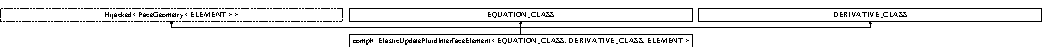
\includegraphics[height=0.707071cm]{classoomph_1_1ElasticUpdateFluidInterfaceElement}
\end{center}
\end{figure}
\subsection*{Public Member Functions}
\begin{DoxyCompactItemize}
\item 
\hyperlink{classoomph_1_1ElasticUpdateFluidInterfaceElement_a5e5d81d8ba6c7b6567ec6d1dd42c1c96}{Elastic\+Update\+Fluid\+Interface\+Element} (\hyperlink{classoomph_1_1FiniteElement}{Finite\+Element} $\ast$const \&element\+\_\+pt, const int \&face\+\_\+index, const unsigned \&id=0)
\begin{DoxyCompactList}\small\item\em Constructor, pass a pointer to the bulk element and the face index of the bulk element to which the element is to be attached to. The optional identifier can be used to distinguish the additional nodal value (Lagr mult) created by this element from those created by other Face\+Elements. \end{DoxyCompactList}\item 
double \hyperlink{classoomph_1_1ElasticUpdateFluidInterfaceElement_a41706192ce4de3c4c51a70086199d8fa}{zeta\+\_\+nodal} (const unsigned \&n, const unsigned \&k, const unsigned \&\hyperlink{cfortran_8h_adb50e893b86b3e55e751a42eab3cba82}{i}) const
\begin{DoxyCompactList}\small\item\em The \char`\"{}global\char`\"{} intrinsic coordinate of the element when viewed as part of a geometric object should be given by the \hyperlink{classoomph_1_1FaceElement}{Face\+Element} representation, by default. \end{DoxyCompactList}\item 
double \& \hyperlink{classoomph_1_1ElasticUpdateFluidInterfaceElement_a8b5c5b703e6daafbe1dcafd3fe93e537}{lagrange} (const unsigned \&n)
\begin{DoxyCompactList}\small\item\em Return the lagrange multiplier at local node n. \end{DoxyCompactList}\item 
void \hyperlink{classoomph_1_1ElasticUpdateFluidInterfaceElement_acc1d5bb57e5664b86a9a76a4cfb8259f}{fill\+\_\+in\+\_\+contribution\+\_\+to\+\_\+jacobian} (\hyperlink{classoomph_1_1Vector}{Vector}$<$ double $>$ \&residuals, \hyperlink{classoomph_1_1DenseMatrix}{Dense\+Matrix}$<$ double $>$ \&jacobian)
\begin{DoxyCompactList}\small\item\em Fill in contribution to residuals and Jacobian. \end{DoxyCompactList}\item 
void \hyperlink{classoomph_1_1ElasticUpdateFluidInterfaceElement_a46b22d178b248355083a3564e4e92eb0}{output} (std\+::ostream \&outfile)
\begin{DoxyCompactList}\small\item\em Overload the output function. \end{DoxyCompactList}\item 
void \hyperlink{classoomph_1_1ElasticUpdateFluidInterfaceElement_ac193aa64a8223a96e4148a5af456fb64}{output} (std\+::ostream \&outfile, const unsigned \&n\+\_\+plot)
\begin{DoxyCompactList}\small\item\em Output the element. \end{DoxyCompactList}\item 
void \hyperlink{classoomph_1_1ElasticUpdateFluidInterfaceElement_a8baae14bdede6a659e948942d7a08cb5}{output} (F\+I\+LE $\ast$file\+\_\+pt)
\begin{DoxyCompactList}\small\item\em Overload the C-\/style output function. \end{DoxyCompactList}\item 
void \hyperlink{classoomph_1_1ElasticUpdateFluidInterfaceElement_a10b64a463b5ff98475e727b06d95b0ac}{output} (F\+I\+LE $\ast$file\+\_\+pt, const unsigned \&n\+\_\+plot)
\begin{DoxyCompactList}\small\item\em C-\/style Output function. \end{DoxyCompactList}\item 
void \hyperlink{classoomph_1_1ElasticUpdateFluidInterfaceElement_a15c3d2912325ace17676366c1469121f}{add\+\_\+additional\+\_\+residual\+\_\+contributions\+\_\+interface} (\hyperlink{classoomph_1_1Vector}{Vector}$<$ double $>$ \&residuals, \hyperlink{classoomph_1_1DenseMatrix}{Dense\+Matrix}$<$ double $>$ \&jacobian, const unsigned \&flag, const \hyperlink{classoomph_1_1Shape}{Shape} \&psif, const \hyperlink{classoomph_1_1DShape}{D\+Shape} \&dpsifds, const \hyperlink{classoomph_1_1DShape}{D\+Shape} \&dpsifdS, const \hyperlink{classoomph_1_1DShape}{D\+Shape} \&dpsifd\+S\+\_\+div, const \hyperlink{classoomph_1_1Vector}{Vector}$<$ double $>$ \&\hyperlink{cfortran_8h_ab7123126e4885ef647dd9c6e3807a21c}{s}, const \hyperlink{classoomph_1_1Vector}{Vector}$<$ double $>$ \&interpolated\+\_\+x, const \hyperlink{classoomph_1_1Vector}{Vector}$<$ double $>$ \&interpolated\+\_\+n, const double \&W, const double \&J)
\begin{DoxyCompactList}\small\item\em Helper function to calculate the additional contributions to be added at each integration point. This deals with Lagrange multiplier contribution, as well as any additional contributions by the other equations. \end{DoxyCompactList}\item 
virtual \hyperlink{classoomph_1_1FluidInterfaceBoundingElement}{Fluid\+Interface\+Bounding\+Element} $\ast$ \hyperlink{classoomph_1_1ElasticUpdateFluidInterfaceElement_a91c59905720a4417447fcce09032ce7f}{make\+\_\+bounding\+\_\+element} (const int \&face\+\_\+index)
\begin{DoxyCompactList}\small\item\em Create an \char`\"{}bounding\char`\"{} element (here actually a 2D line element of type Elastic\+Line\+Fluid\+Interface\+Bounding\+Element$<$\+E\+L\+E\+M\+E\+N\+T$>$ that allows the application of a contact angle boundary condition on the the specified face. \end{DoxyCompactList}\end{DoxyCompactItemize}
\subsection*{Protected Member Functions}
\begin{DoxyCompactItemize}
\item 
double \hyperlink{classoomph_1_1ElasticUpdateFluidInterfaceElement_ae9df6c11ccb63dc04c0d5ca655fe1482}{compute\+\_\+surface\+\_\+derivatives} (const \hyperlink{classoomph_1_1Shape}{Shape} \&psi, const \hyperlink{classoomph_1_1DShape}{D\+Shape} \&dpsids, const \hyperlink{classoomph_1_1DenseMatrix}{Dense\+Matrix}$<$ double $>$ \&interpolated\+\_\+t, const \hyperlink{classoomph_1_1Vector}{Vector}$<$ double $>$ \&interpolated\+\_\+x, \hyperlink{classoomph_1_1DShape}{D\+Shape} \&surface\+\_\+gradient, \hyperlink{classoomph_1_1DShape}{D\+Shape} \&surface\+\_\+divergence)
\begin{DoxyCompactList}\small\item\em Fill in the specific surface derivative calculations by calling the appropriate function from the derivative class. \end{DoxyCompactList}\end{DoxyCompactItemize}
\subsection*{Private Member Functions}
\begin{DoxyCompactItemize}
\item 
unsigned \hyperlink{classoomph_1_1ElasticUpdateFluidInterfaceElement_a2eb4fbe50ac4ff1e9b26e0e1d8ff3186}{lagrange\+\_\+index} (const unsigned \&n)
\begin{DoxyCompactList}\small\item\em Return the index at which the lagrange multiplier is stored at the n-\/th node. \end{DoxyCompactList}\item 
int \hyperlink{classoomph_1_1ElasticUpdateFluidInterfaceElement_a940840693906b7b8d619ff97f521c811}{kinematic\+\_\+local\+\_\+eqn} (const unsigned \&n)
\begin{DoxyCompactList}\small\item\em Equation number of the kinematic BC associated with node j. (This is the equation for the Lagrange multiplier) \end{DoxyCompactList}\item 
void \hyperlink{classoomph_1_1ElasticUpdateFluidInterfaceElement_ae82f486496a0647d905ab6ee857de0d0}{hijack\+\_\+kinematic\+\_\+conditions} (const \hyperlink{classoomph_1_1Vector}{Vector}$<$ unsigned $>$ \&bulk\+\_\+node\+\_\+number)
\begin{DoxyCompactList}\small\item\em Hijacking the kinematic condition corresponds to hijacking the variables associated with the Lagrange multipliers that are assigned on construction of this element. \end{DoxyCompactList}\end{DoxyCompactItemize}
\subsection*{Private Attributes}
\begin{DoxyCompactItemize}
\item 
\hyperlink{classoomph_1_1Vector}{Vector}$<$ unsigned $>$ \hyperlink{classoomph_1_1ElasticUpdateFluidInterfaceElement_a7852050a89e3aac51ed3693814be9018}{Lagrange\+\_\+index}
\begin{DoxyCompactList}\small\item\em Storage for the location of the Lagrange multiplier (If other additional values have been added we need to add the Lagrange multiplier at the end) \end{DoxyCompactList}\end{DoxyCompactItemize}
\subsection*{Additional Inherited Members}


\subsection{Detailed Description}
\subsubsection*{template$<$class E\+Q\+U\+A\+T\+I\+O\+N\+\_\+\+C\+L\+A\+SS, class D\+E\+R\+I\+V\+A\+T\+I\+V\+E\+\_\+\+C\+L\+A\+SS, class E\+L\+E\+M\+E\+NT$>$\newline
class oomph\+::\+Elastic\+Update\+Fluid\+Interface\+Element$<$ E\+Q\+U\+A\+T\+I\+O\+N\+\_\+\+C\+L\+A\+S\+S, D\+E\+R\+I\+V\+A\+T\+I\+V\+E\+\_\+\+C\+L\+A\+S\+S, E\+L\+E\+M\+E\+N\+T $>$}

Generic Elastic node update interface template class that can be combined with a given surface equations class and surface derivative class to provide a concrete implementation of any surface element that uses elastic node updates. 

Definition at line 595 of file specific\+\_\+node\+\_\+update\+\_\+interface\+\_\+elements.\+h.



\subsection{Constructor \& Destructor Documentation}
\mbox{\Hypertarget{classoomph_1_1ElasticUpdateFluidInterfaceElement_a5e5d81d8ba6c7b6567ec6d1dd42c1c96}\label{classoomph_1_1ElasticUpdateFluidInterfaceElement_a5e5d81d8ba6c7b6567ec6d1dd42c1c96}} 
\index{oomph\+::\+Elastic\+Update\+Fluid\+Interface\+Element@{oomph\+::\+Elastic\+Update\+Fluid\+Interface\+Element}!Elastic\+Update\+Fluid\+Interface\+Element@{Elastic\+Update\+Fluid\+Interface\+Element}}
\index{Elastic\+Update\+Fluid\+Interface\+Element@{Elastic\+Update\+Fluid\+Interface\+Element}!oomph\+::\+Elastic\+Update\+Fluid\+Interface\+Element@{oomph\+::\+Elastic\+Update\+Fluid\+Interface\+Element}}
\subsubsection{\texorpdfstring{Elastic\+Update\+Fluid\+Interface\+Element()}{ElasticUpdateFluidInterfaceElement()}}
{\footnotesize\ttfamily template$<$class E\+Q\+U\+A\+T\+I\+O\+N\+\_\+\+C\+L\+A\+SS, class D\+E\+R\+I\+V\+A\+T\+I\+V\+E\+\_\+\+C\+L\+A\+SS, class E\+L\+E\+M\+E\+NT$>$ \\
\hyperlink{classoomph_1_1ElasticUpdateFluidInterfaceElement}{oomph\+::\+Elastic\+Update\+Fluid\+Interface\+Element}$<$ E\+Q\+U\+A\+T\+I\+O\+N\+\_\+\+C\+L\+A\+SS, D\+E\+R\+I\+V\+A\+T\+I\+V\+E\+\_\+\+C\+L\+A\+SS, E\+L\+E\+M\+E\+NT $>$\+::\hyperlink{classoomph_1_1ElasticUpdateFluidInterfaceElement}{Elastic\+Update\+Fluid\+Interface\+Element} (\begin{DoxyParamCaption}\item[{\hyperlink{classoomph_1_1FiniteElement}{Finite\+Element} $\ast$const \&}]{element\+\_\+pt,  }\item[{const int \&}]{face\+\_\+index,  }\item[{const unsigned \&}]{id = {\ttfamily 0} }\end{DoxyParamCaption})\hspace{0.3cm}{\ttfamily [inline]}}



Constructor, pass a pointer to the bulk element and the face index of the bulk element to which the element is to be attached to. The optional identifier can be used to distinguish the additional nodal value (Lagr mult) created by this element from those created by other Face\+Elements. 



Definition at line 654 of file specific\+\_\+node\+\_\+update\+\_\+interface\+\_\+elements.\+h.



\subsection{Member Function Documentation}
\mbox{\Hypertarget{classoomph_1_1ElasticUpdateFluidInterfaceElement_a15c3d2912325ace17676366c1469121f}\label{classoomph_1_1ElasticUpdateFluidInterfaceElement_a15c3d2912325ace17676366c1469121f}} 
\index{oomph\+::\+Elastic\+Update\+Fluid\+Interface\+Element@{oomph\+::\+Elastic\+Update\+Fluid\+Interface\+Element}!add\+\_\+additional\+\_\+residual\+\_\+contributions\+\_\+interface@{add\+\_\+additional\+\_\+residual\+\_\+contributions\+\_\+interface}}
\index{add\+\_\+additional\+\_\+residual\+\_\+contributions\+\_\+interface@{add\+\_\+additional\+\_\+residual\+\_\+contributions\+\_\+interface}!oomph\+::\+Elastic\+Update\+Fluid\+Interface\+Element@{oomph\+::\+Elastic\+Update\+Fluid\+Interface\+Element}}
\subsubsection{\texorpdfstring{add\+\_\+additional\+\_\+residual\+\_\+contributions\+\_\+interface()}{add\_additional\_residual\_contributions\_interface()}}
{\footnotesize\ttfamily template$<$class E\+Q\+U\+A\+T\+I\+O\+N\+\_\+\+C\+L\+A\+SS, class D\+E\+R\+I\+V\+A\+T\+I\+V\+E\+\_\+\+C\+L\+A\+SS, class E\+L\+E\+M\+E\+NT$>$ \\
void \hyperlink{classoomph_1_1ElasticUpdateFluidInterfaceElement}{oomph\+::\+Elastic\+Update\+Fluid\+Interface\+Element}$<$ E\+Q\+U\+A\+T\+I\+O\+N\+\_\+\+C\+L\+A\+SS, D\+E\+R\+I\+V\+A\+T\+I\+V\+E\+\_\+\+C\+L\+A\+SS, E\+L\+E\+M\+E\+NT $>$\+::add\+\_\+additional\+\_\+residual\+\_\+contributions\+\_\+interface (\begin{DoxyParamCaption}\item[{\hyperlink{classoomph_1_1Vector}{Vector}$<$ double $>$ \&}]{residuals,  }\item[{\hyperlink{classoomph_1_1DenseMatrix}{Dense\+Matrix}$<$ double $>$ \&}]{jacobian,  }\item[{const unsigned \&}]{flag,  }\item[{const \hyperlink{classoomph_1_1Shape}{Shape} \&}]{psif,  }\item[{const \hyperlink{classoomph_1_1DShape}{D\+Shape} \&}]{dpsifds,  }\item[{const \hyperlink{classoomph_1_1DShape}{D\+Shape} \&}]{dpsifdS,  }\item[{const \hyperlink{classoomph_1_1DShape}{D\+Shape} \&}]{dpsifd\+S\+\_\+div,  }\item[{const \hyperlink{classoomph_1_1Vector}{Vector}$<$ double $>$ \&}]{s,  }\item[{const \hyperlink{classoomph_1_1Vector}{Vector}$<$ double $>$ \&}]{interpolated\+\_\+x,  }\item[{const \hyperlink{classoomph_1_1Vector}{Vector}$<$ double $>$ \&}]{interpolated\+\_\+n,  }\item[{const double \&}]{W,  }\item[{const double \&}]{J }\end{DoxyParamCaption})\hspace{0.3cm}{\ttfamily [inline]}}



Helper function to calculate the additional contributions to be added at each integration point. This deals with Lagrange multiplier contribution, as well as any additional contributions by the other equations. 



Definition at line 772 of file specific\+\_\+node\+\_\+update\+\_\+interface\+\_\+elements.\+h.

\mbox{\Hypertarget{classoomph_1_1ElasticUpdateFluidInterfaceElement_ae9df6c11ccb63dc04c0d5ca655fe1482}\label{classoomph_1_1ElasticUpdateFluidInterfaceElement_ae9df6c11ccb63dc04c0d5ca655fe1482}} 
\index{oomph\+::\+Elastic\+Update\+Fluid\+Interface\+Element@{oomph\+::\+Elastic\+Update\+Fluid\+Interface\+Element}!compute\+\_\+surface\+\_\+derivatives@{compute\+\_\+surface\+\_\+derivatives}}
\index{compute\+\_\+surface\+\_\+derivatives@{compute\+\_\+surface\+\_\+derivatives}!oomph\+::\+Elastic\+Update\+Fluid\+Interface\+Element@{oomph\+::\+Elastic\+Update\+Fluid\+Interface\+Element}}
\subsubsection{\texorpdfstring{compute\+\_\+surface\+\_\+derivatives()}{compute\_surface\_derivatives()}}
{\footnotesize\ttfamily template$<$class E\+Q\+U\+A\+T\+I\+O\+N\+\_\+\+C\+L\+A\+SS, class D\+E\+R\+I\+V\+A\+T\+I\+V\+E\+\_\+\+C\+L\+A\+SS, class E\+L\+E\+M\+E\+NT$>$ \\
double \hyperlink{classoomph_1_1ElasticUpdateFluidInterfaceElement}{oomph\+::\+Elastic\+Update\+Fluid\+Interface\+Element}$<$ E\+Q\+U\+A\+T\+I\+O\+N\+\_\+\+C\+L\+A\+SS, D\+E\+R\+I\+V\+A\+T\+I\+V\+E\+\_\+\+C\+L\+A\+SS, E\+L\+E\+M\+E\+NT $>$\+::compute\+\_\+surface\+\_\+derivatives (\begin{DoxyParamCaption}\item[{const \hyperlink{classoomph_1_1Shape}{Shape} \&}]{psi,  }\item[{const \hyperlink{classoomph_1_1DShape}{D\+Shape} \&}]{dpsids,  }\item[{const \hyperlink{classoomph_1_1DenseMatrix}{Dense\+Matrix}$<$ double $>$ \&}]{interpolated\+\_\+t,  }\item[{const \hyperlink{classoomph_1_1Vector}{Vector}$<$ double $>$ \&}]{interpolated\+\_\+x,  }\item[{\hyperlink{classoomph_1_1DShape}{D\+Shape} \&}]{surface\+\_\+gradient,  }\item[{\hyperlink{classoomph_1_1DShape}{D\+Shape} \&}]{surface\+\_\+divergence }\end{DoxyParamCaption})\hspace{0.3cm}{\ttfamily [inline]}, {\ttfamily [protected]}}



Fill in the specific surface derivative calculations by calling the appropriate function from the derivative class. 



Definition at line 637 of file specific\+\_\+node\+\_\+update\+\_\+interface\+\_\+elements.\+h.

\mbox{\Hypertarget{classoomph_1_1ElasticUpdateFluidInterfaceElement_acc1d5bb57e5664b86a9a76a4cfb8259f}\label{classoomph_1_1ElasticUpdateFluidInterfaceElement_acc1d5bb57e5664b86a9a76a4cfb8259f}} 
\index{oomph\+::\+Elastic\+Update\+Fluid\+Interface\+Element@{oomph\+::\+Elastic\+Update\+Fluid\+Interface\+Element}!fill\+\_\+in\+\_\+contribution\+\_\+to\+\_\+jacobian@{fill\+\_\+in\+\_\+contribution\+\_\+to\+\_\+jacobian}}
\index{fill\+\_\+in\+\_\+contribution\+\_\+to\+\_\+jacobian@{fill\+\_\+in\+\_\+contribution\+\_\+to\+\_\+jacobian}!oomph\+::\+Elastic\+Update\+Fluid\+Interface\+Element@{oomph\+::\+Elastic\+Update\+Fluid\+Interface\+Element}}
\subsubsection{\texorpdfstring{fill\+\_\+in\+\_\+contribution\+\_\+to\+\_\+jacobian()}{fill\_in\_contribution\_to\_jacobian()}}
{\footnotesize\ttfamily template$<$class E\+Q\+U\+A\+T\+I\+O\+N\+\_\+\+C\+L\+A\+SS, class D\+E\+R\+I\+V\+A\+T\+I\+V\+E\+\_\+\+C\+L\+A\+SS, class E\+L\+E\+M\+E\+NT$>$ \\
void \hyperlink{classoomph_1_1ElasticUpdateFluidInterfaceElement}{oomph\+::\+Elastic\+Update\+Fluid\+Interface\+Element}$<$ E\+Q\+U\+A\+T\+I\+O\+N\+\_\+\+C\+L\+A\+SS, D\+E\+R\+I\+V\+A\+T\+I\+V\+E\+\_\+\+C\+L\+A\+SS, E\+L\+E\+M\+E\+NT $>$\+::fill\+\_\+in\+\_\+contribution\+\_\+to\+\_\+jacobian (\begin{DoxyParamCaption}\item[{\hyperlink{classoomph_1_1Vector}{Vector}$<$ double $>$ \&}]{residuals,  }\item[{\hyperlink{classoomph_1_1DenseMatrix}{Dense\+Matrix}$<$ double $>$ \&}]{jacobian }\end{DoxyParamCaption})\hspace{0.3cm}{\ttfamily [inline]}}



Fill in contribution to residuals and Jacobian. 



Definition at line 743 of file specific\+\_\+node\+\_\+update\+\_\+interface\+\_\+elements.\+h.

\mbox{\Hypertarget{classoomph_1_1ElasticUpdateFluidInterfaceElement_ae82f486496a0647d905ab6ee857de0d0}\label{classoomph_1_1ElasticUpdateFluidInterfaceElement_ae82f486496a0647d905ab6ee857de0d0}} 
\index{oomph\+::\+Elastic\+Update\+Fluid\+Interface\+Element@{oomph\+::\+Elastic\+Update\+Fluid\+Interface\+Element}!hijack\+\_\+kinematic\+\_\+conditions@{hijack\+\_\+kinematic\+\_\+conditions}}
\index{hijack\+\_\+kinematic\+\_\+conditions@{hijack\+\_\+kinematic\+\_\+conditions}!oomph\+::\+Elastic\+Update\+Fluid\+Interface\+Element@{oomph\+::\+Elastic\+Update\+Fluid\+Interface\+Element}}
\subsubsection{\texorpdfstring{hijack\+\_\+kinematic\+\_\+conditions()}{hijack\_kinematic\_conditions()}}
{\footnotesize\ttfamily template$<$class E\+Q\+U\+A\+T\+I\+O\+N\+\_\+\+C\+L\+A\+SS, class D\+E\+R\+I\+V\+A\+T\+I\+V\+E\+\_\+\+C\+L\+A\+SS, class E\+L\+E\+M\+E\+NT$>$ \\
void \hyperlink{classoomph_1_1ElasticUpdateFluidInterfaceElement}{oomph\+::\+Elastic\+Update\+Fluid\+Interface\+Element}$<$ E\+Q\+U\+A\+T\+I\+O\+N\+\_\+\+C\+L\+A\+SS, D\+E\+R\+I\+V\+A\+T\+I\+V\+E\+\_\+\+C\+L\+A\+SS, E\+L\+E\+M\+E\+NT $>$\+::hijack\+\_\+kinematic\+\_\+conditions (\begin{DoxyParamCaption}\item[{const \hyperlink{classoomph_1_1Vector}{Vector}$<$ unsigned $>$ \&}]{bulk\+\_\+node\+\_\+number }\end{DoxyParamCaption})\hspace{0.3cm}{\ttfamily [inline]}, {\ttfamily [private]}}



Hijacking the kinematic condition corresponds to hijacking the variables associated with the Lagrange multipliers that are assigned on construction of this element. 



Definition at line 622 of file specific\+\_\+node\+\_\+update\+\_\+interface\+\_\+elements.\+h.

\mbox{\Hypertarget{classoomph_1_1ElasticUpdateFluidInterfaceElement_a940840693906b7b8d619ff97f521c811}\label{classoomph_1_1ElasticUpdateFluidInterfaceElement_a940840693906b7b8d619ff97f521c811}} 
\index{oomph\+::\+Elastic\+Update\+Fluid\+Interface\+Element@{oomph\+::\+Elastic\+Update\+Fluid\+Interface\+Element}!kinematic\+\_\+local\+\_\+eqn@{kinematic\+\_\+local\+\_\+eqn}}
\index{kinematic\+\_\+local\+\_\+eqn@{kinematic\+\_\+local\+\_\+eqn}!oomph\+::\+Elastic\+Update\+Fluid\+Interface\+Element@{oomph\+::\+Elastic\+Update\+Fluid\+Interface\+Element}}
\subsubsection{\texorpdfstring{kinematic\+\_\+local\+\_\+eqn()}{kinematic\_local\_eqn()}}
{\footnotesize\ttfamily template$<$class E\+Q\+U\+A\+T\+I\+O\+N\+\_\+\+C\+L\+A\+SS, class D\+E\+R\+I\+V\+A\+T\+I\+V\+E\+\_\+\+C\+L\+A\+SS, class E\+L\+E\+M\+E\+NT$>$ \\
int \hyperlink{classoomph_1_1ElasticUpdateFluidInterfaceElement}{oomph\+::\+Elastic\+Update\+Fluid\+Interface\+Element}$<$ E\+Q\+U\+A\+T\+I\+O\+N\+\_\+\+C\+L\+A\+SS, D\+E\+R\+I\+V\+A\+T\+I\+V\+E\+\_\+\+C\+L\+A\+SS, E\+L\+E\+M\+E\+NT $>$\+::kinematic\+\_\+local\+\_\+eqn (\begin{DoxyParamCaption}\item[{const unsigned \&}]{n }\end{DoxyParamCaption})\hspace{0.3cm}{\ttfamily [inline]}, {\ttfamily [private]}}



Equation number of the kinematic BC associated with node j. (This is the equation for the Lagrange multiplier) 



Definition at line 613 of file specific\+\_\+node\+\_\+update\+\_\+interface\+\_\+elements.\+h.

\mbox{\Hypertarget{classoomph_1_1ElasticUpdateFluidInterfaceElement_a8b5c5b703e6daafbe1dcafd3fe93e537}\label{classoomph_1_1ElasticUpdateFluidInterfaceElement_a8b5c5b703e6daafbe1dcafd3fe93e537}} 
\index{oomph\+::\+Elastic\+Update\+Fluid\+Interface\+Element@{oomph\+::\+Elastic\+Update\+Fluid\+Interface\+Element}!lagrange@{lagrange}}
\index{lagrange@{lagrange}!oomph\+::\+Elastic\+Update\+Fluid\+Interface\+Element@{oomph\+::\+Elastic\+Update\+Fluid\+Interface\+Element}}
\subsubsection{\texorpdfstring{lagrange()}{lagrange()}}
{\footnotesize\ttfamily template$<$class E\+Q\+U\+A\+T\+I\+O\+N\+\_\+\+C\+L\+A\+SS, class D\+E\+R\+I\+V\+A\+T\+I\+V\+E\+\_\+\+C\+L\+A\+SS, class E\+L\+E\+M\+E\+NT$>$ \\
double\& \hyperlink{classoomph_1_1ElasticUpdateFluidInterfaceElement}{oomph\+::\+Elastic\+Update\+Fluid\+Interface\+Element}$<$ E\+Q\+U\+A\+T\+I\+O\+N\+\_\+\+C\+L\+A\+SS, D\+E\+R\+I\+V\+A\+T\+I\+V\+E\+\_\+\+C\+L\+A\+SS, E\+L\+E\+M\+E\+NT $>$\+::lagrange (\begin{DoxyParamCaption}\item[{const unsigned \&}]{n }\end{DoxyParamCaption})\hspace{0.3cm}{\ttfamily [inline]}}



Return the lagrange multiplier at local node n. 



Definition at line 736 of file specific\+\_\+node\+\_\+update\+\_\+interface\+\_\+elements.\+h.

\mbox{\Hypertarget{classoomph_1_1ElasticUpdateFluidInterfaceElement_a2eb4fbe50ac4ff1e9b26e0e1d8ff3186}\label{classoomph_1_1ElasticUpdateFluidInterfaceElement_a2eb4fbe50ac4ff1e9b26e0e1d8ff3186}} 
\index{oomph\+::\+Elastic\+Update\+Fluid\+Interface\+Element@{oomph\+::\+Elastic\+Update\+Fluid\+Interface\+Element}!lagrange\+\_\+index@{lagrange\+\_\+index}}
\index{lagrange\+\_\+index@{lagrange\+\_\+index}!oomph\+::\+Elastic\+Update\+Fluid\+Interface\+Element@{oomph\+::\+Elastic\+Update\+Fluid\+Interface\+Element}}
\subsubsection{\texorpdfstring{lagrange\+\_\+index()}{lagrange\_index()}}
{\footnotesize\ttfamily template$<$class E\+Q\+U\+A\+T\+I\+O\+N\+\_\+\+C\+L\+A\+SS, class D\+E\+R\+I\+V\+A\+T\+I\+V\+E\+\_\+\+C\+L\+A\+SS, class E\+L\+E\+M\+E\+NT$>$ \\
unsigned \hyperlink{classoomph_1_1ElasticUpdateFluidInterfaceElement}{oomph\+::\+Elastic\+Update\+Fluid\+Interface\+Element}$<$ E\+Q\+U\+A\+T\+I\+O\+N\+\_\+\+C\+L\+A\+SS, D\+E\+R\+I\+V\+A\+T\+I\+V\+E\+\_\+\+C\+L\+A\+SS, E\+L\+E\+M\+E\+NT $>$\+::lagrange\+\_\+index (\begin{DoxyParamCaption}\item[{const unsigned \&}]{n }\end{DoxyParamCaption})\hspace{0.3cm}{\ttfamily [inline]}, {\ttfamily [private]}}



Return the index at which the lagrange multiplier is stored at the n-\/th node. 



Definition at line 608 of file specific\+\_\+node\+\_\+update\+\_\+interface\+\_\+elements.\+h.

\mbox{\Hypertarget{classoomph_1_1ElasticUpdateFluidInterfaceElement_a91c59905720a4417447fcce09032ce7f}\label{classoomph_1_1ElasticUpdateFluidInterfaceElement_a91c59905720a4417447fcce09032ce7f}} 
\index{oomph\+::\+Elastic\+Update\+Fluid\+Interface\+Element@{oomph\+::\+Elastic\+Update\+Fluid\+Interface\+Element}!make\+\_\+bounding\+\_\+element@{make\+\_\+bounding\+\_\+element}}
\index{make\+\_\+bounding\+\_\+element@{make\+\_\+bounding\+\_\+element}!oomph\+::\+Elastic\+Update\+Fluid\+Interface\+Element@{oomph\+::\+Elastic\+Update\+Fluid\+Interface\+Element}}
\subsubsection{\texorpdfstring{make\+\_\+bounding\+\_\+element()}{make\_bounding\_element()}}
{\footnotesize\ttfamily template$<$class E\+Q\+U\+A\+T\+I\+O\+N\+\_\+\+C\+L\+A\+SS, class D\+E\+R\+I\+V\+A\+T\+I\+V\+E\+\_\+\+C\+L\+A\+SS, class E\+L\+E\+M\+E\+NT$>$ \\
virtual \hyperlink{classoomph_1_1FluidInterfaceBoundingElement}{Fluid\+Interface\+Bounding\+Element}$\ast$ \hyperlink{classoomph_1_1ElasticUpdateFluidInterfaceElement}{oomph\+::\+Elastic\+Update\+Fluid\+Interface\+Element}$<$ E\+Q\+U\+A\+T\+I\+O\+N\+\_\+\+C\+L\+A\+SS, D\+E\+R\+I\+V\+A\+T\+I\+V\+E\+\_\+\+C\+L\+A\+SS, E\+L\+E\+M\+E\+NT $>$\+::make\+\_\+bounding\+\_\+element (\begin{DoxyParamCaption}\item[{const int \&}]{face\+\_\+index }\end{DoxyParamCaption})\hspace{0.3cm}{\ttfamily [inline]}, {\ttfamily [virtual]}}



Create an \char`\"{}bounding\char`\"{} element (here actually a 2D line element of type Elastic\+Line\+Fluid\+Interface\+Bounding\+Element$<$\+E\+L\+E\+M\+E\+N\+T$>$ that allows the application of a contact angle boundary condition on the the specified face. 



Definition at line 846 of file specific\+\_\+node\+\_\+update\+\_\+interface\+\_\+elements.\+h.

\mbox{\Hypertarget{classoomph_1_1ElasticUpdateFluidInterfaceElement_a46b22d178b248355083a3564e4e92eb0}\label{classoomph_1_1ElasticUpdateFluidInterfaceElement_a46b22d178b248355083a3564e4e92eb0}} 
\index{oomph\+::\+Elastic\+Update\+Fluid\+Interface\+Element@{oomph\+::\+Elastic\+Update\+Fluid\+Interface\+Element}!output@{output}}
\index{output@{output}!oomph\+::\+Elastic\+Update\+Fluid\+Interface\+Element@{oomph\+::\+Elastic\+Update\+Fluid\+Interface\+Element}}
\subsubsection{\texorpdfstring{output()}{output()}\hspace{0.1cm}{\footnotesize\ttfamily [1/4]}}
{\footnotesize\ttfamily template$<$class E\+Q\+U\+A\+T\+I\+O\+N\+\_\+\+C\+L\+A\+SS, class D\+E\+R\+I\+V\+A\+T\+I\+V\+E\+\_\+\+C\+L\+A\+SS, class E\+L\+E\+M\+E\+NT$>$ \\
void \hyperlink{classoomph_1_1ElasticUpdateFluidInterfaceElement}{oomph\+::\+Elastic\+Update\+Fluid\+Interface\+Element}$<$ E\+Q\+U\+A\+T\+I\+O\+N\+\_\+\+C\+L\+A\+SS, D\+E\+R\+I\+V\+A\+T\+I\+V\+E\+\_\+\+C\+L\+A\+SS, E\+L\+E\+M\+E\+NT $>$\+::output (\begin{DoxyParamCaption}\item[{std\+::ostream \&}]{outfile }\end{DoxyParamCaption})\hspace{0.3cm}{\ttfamily [inline]}}



Overload the output function. 



Definition at line 754 of file specific\+\_\+node\+\_\+update\+\_\+interface\+\_\+elements.\+h.

\mbox{\Hypertarget{classoomph_1_1ElasticUpdateFluidInterfaceElement_ac193aa64a8223a96e4148a5af456fb64}\label{classoomph_1_1ElasticUpdateFluidInterfaceElement_ac193aa64a8223a96e4148a5af456fb64}} 
\index{oomph\+::\+Elastic\+Update\+Fluid\+Interface\+Element@{oomph\+::\+Elastic\+Update\+Fluid\+Interface\+Element}!output@{output}}
\index{output@{output}!oomph\+::\+Elastic\+Update\+Fluid\+Interface\+Element@{oomph\+::\+Elastic\+Update\+Fluid\+Interface\+Element}}
\subsubsection{\texorpdfstring{output()}{output()}\hspace{0.1cm}{\footnotesize\ttfamily [2/4]}}
{\footnotesize\ttfamily template$<$class E\+Q\+U\+A\+T\+I\+O\+N\+\_\+\+C\+L\+A\+SS, class D\+E\+R\+I\+V\+A\+T\+I\+V\+E\+\_\+\+C\+L\+A\+SS, class E\+L\+E\+M\+E\+NT$>$ \\
void \hyperlink{classoomph_1_1ElasticUpdateFluidInterfaceElement}{oomph\+::\+Elastic\+Update\+Fluid\+Interface\+Element}$<$ E\+Q\+U\+A\+T\+I\+O\+N\+\_\+\+C\+L\+A\+SS, D\+E\+R\+I\+V\+A\+T\+I\+V\+E\+\_\+\+C\+L\+A\+SS, E\+L\+E\+M\+E\+NT $>$\+::output (\begin{DoxyParamCaption}\item[{std\+::ostream \&}]{outfile,  }\item[{const unsigned \&}]{n\+\_\+plot }\end{DoxyParamCaption})\hspace{0.3cm}{\ttfamily [inline]}}



Output the element. 



Definition at line 757 of file specific\+\_\+node\+\_\+update\+\_\+interface\+\_\+elements.\+h.

\mbox{\Hypertarget{classoomph_1_1ElasticUpdateFluidInterfaceElement_a8baae14bdede6a659e948942d7a08cb5}\label{classoomph_1_1ElasticUpdateFluidInterfaceElement_a8baae14bdede6a659e948942d7a08cb5}} 
\index{oomph\+::\+Elastic\+Update\+Fluid\+Interface\+Element@{oomph\+::\+Elastic\+Update\+Fluid\+Interface\+Element}!output@{output}}
\index{output@{output}!oomph\+::\+Elastic\+Update\+Fluid\+Interface\+Element@{oomph\+::\+Elastic\+Update\+Fluid\+Interface\+Element}}
\subsubsection{\texorpdfstring{output()}{output()}\hspace{0.1cm}{\footnotesize\ttfamily [3/4]}}
{\footnotesize\ttfamily template$<$class E\+Q\+U\+A\+T\+I\+O\+N\+\_\+\+C\+L\+A\+SS, class D\+E\+R\+I\+V\+A\+T\+I\+V\+E\+\_\+\+C\+L\+A\+SS, class E\+L\+E\+M\+E\+NT$>$ \\
void \hyperlink{classoomph_1_1ElasticUpdateFluidInterfaceElement}{oomph\+::\+Elastic\+Update\+Fluid\+Interface\+Element}$<$ E\+Q\+U\+A\+T\+I\+O\+N\+\_\+\+C\+L\+A\+SS, D\+E\+R\+I\+V\+A\+T\+I\+V\+E\+\_\+\+C\+L\+A\+SS, E\+L\+E\+M\+E\+NT $>$\+::output (\begin{DoxyParamCaption}\item[{F\+I\+LE $\ast$}]{file\+\_\+pt }\end{DoxyParamCaption})\hspace{0.3cm}{\ttfamily [inline]}}



Overload the C-\/style output function. 



Definition at line 761 of file specific\+\_\+node\+\_\+update\+\_\+interface\+\_\+elements.\+h.

\mbox{\Hypertarget{classoomph_1_1ElasticUpdateFluidInterfaceElement_a10b64a463b5ff98475e727b06d95b0ac}\label{classoomph_1_1ElasticUpdateFluidInterfaceElement_a10b64a463b5ff98475e727b06d95b0ac}} 
\index{oomph\+::\+Elastic\+Update\+Fluid\+Interface\+Element@{oomph\+::\+Elastic\+Update\+Fluid\+Interface\+Element}!output@{output}}
\index{output@{output}!oomph\+::\+Elastic\+Update\+Fluid\+Interface\+Element@{oomph\+::\+Elastic\+Update\+Fluid\+Interface\+Element}}
\subsubsection{\texorpdfstring{output()}{output()}\hspace{0.1cm}{\footnotesize\ttfamily [4/4]}}
{\footnotesize\ttfamily template$<$class E\+Q\+U\+A\+T\+I\+O\+N\+\_\+\+C\+L\+A\+SS, class D\+E\+R\+I\+V\+A\+T\+I\+V\+E\+\_\+\+C\+L\+A\+SS, class E\+L\+E\+M\+E\+NT$>$ \\
void \hyperlink{classoomph_1_1ElasticUpdateFluidInterfaceElement}{oomph\+::\+Elastic\+Update\+Fluid\+Interface\+Element}$<$ E\+Q\+U\+A\+T\+I\+O\+N\+\_\+\+C\+L\+A\+SS, D\+E\+R\+I\+V\+A\+T\+I\+V\+E\+\_\+\+C\+L\+A\+SS, E\+L\+E\+M\+E\+NT $>$\+::output (\begin{DoxyParamCaption}\item[{F\+I\+LE $\ast$}]{file\+\_\+pt,  }\item[{const unsigned \&}]{n\+\_\+plot }\end{DoxyParamCaption})\hspace{0.3cm}{\ttfamily [inline]}}



C-\/style Output function. 



Definition at line 764 of file specific\+\_\+node\+\_\+update\+\_\+interface\+\_\+elements.\+h.

\mbox{\Hypertarget{classoomph_1_1ElasticUpdateFluidInterfaceElement_a41706192ce4de3c4c51a70086199d8fa}\label{classoomph_1_1ElasticUpdateFluidInterfaceElement_a41706192ce4de3c4c51a70086199d8fa}} 
\index{oomph\+::\+Elastic\+Update\+Fluid\+Interface\+Element@{oomph\+::\+Elastic\+Update\+Fluid\+Interface\+Element}!zeta\+\_\+nodal@{zeta\+\_\+nodal}}
\index{zeta\+\_\+nodal@{zeta\+\_\+nodal}!oomph\+::\+Elastic\+Update\+Fluid\+Interface\+Element@{oomph\+::\+Elastic\+Update\+Fluid\+Interface\+Element}}
\subsubsection{\texorpdfstring{zeta\+\_\+nodal()}{zeta\_nodal()}}
{\footnotesize\ttfamily template$<$class E\+Q\+U\+A\+T\+I\+O\+N\+\_\+\+C\+L\+A\+SS, class D\+E\+R\+I\+V\+A\+T\+I\+V\+E\+\_\+\+C\+L\+A\+SS, class E\+L\+E\+M\+E\+NT$>$ \\
double \hyperlink{classoomph_1_1ElasticUpdateFluidInterfaceElement}{oomph\+::\+Elastic\+Update\+Fluid\+Interface\+Element}$<$ E\+Q\+U\+A\+T\+I\+O\+N\+\_\+\+C\+L\+A\+SS, D\+E\+R\+I\+V\+A\+T\+I\+V\+E\+\_\+\+C\+L\+A\+SS, E\+L\+E\+M\+E\+NT $>$\+::zeta\+\_\+nodal (\begin{DoxyParamCaption}\item[{const unsigned \&}]{n,  }\item[{const unsigned \&}]{k,  }\item[{const unsigned \&}]{i }\end{DoxyParamCaption}) const\hspace{0.3cm}{\ttfamily [inline]}}



The \char`\"{}global\char`\"{} intrinsic coordinate of the element when viewed as part of a geometric object should be given by the \hyperlink{classoomph_1_1FaceElement}{Face\+Element} representation, by default. 



Definition at line 731 of file specific\+\_\+node\+\_\+update\+\_\+interface\+\_\+elements.\+h.



\subsection{Member Data Documentation}
\mbox{\Hypertarget{classoomph_1_1ElasticUpdateFluidInterfaceElement_a7852050a89e3aac51ed3693814be9018}\label{classoomph_1_1ElasticUpdateFluidInterfaceElement_a7852050a89e3aac51ed3693814be9018}} 
\index{oomph\+::\+Elastic\+Update\+Fluid\+Interface\+Element@{oomph\+::\+Elastic\+Update\+Fluid\+Interface\+Element}!Lagrange\+\_\+index@{Lagrange\+\_\+index}}
\index{Lagrange\+\_\+index@{Lagrange\+\_\+index}!oomph\+::\+Elastic\+Update\+Fluid\+Interface\+Element@{oomph\+::\+Elastic\+Update\+Fluid\+Interface\+Element}}
\subsubsection{\texorpdfstring{Lagrange\+\_\+index}{Lagrange\_index}}
{\footnotesize\ttfamily template$<$class E\+Q\+U\+A\+T\+I\+O\+N\+\_\+\+C\+L\+A\+SS, class D\+E\+R\+I\+V\+A\+T\+I\+V\+E\+\_\+\+C\+L\+A\+SS, class E\+L\+E\+M\+E\+NT$>$ \\
\hyperlink{classoomph_1_1Vector}{Vector}$<$unsigned$>$ \hyperlink{classoomph_1_1ElasticUpdateFluidInterfaceElement}{oomph\+::\+Elastic\+Update\+Fluid\+Interface\+Element}$<$ E\+Q\+U\+A\+T\+I\+O\+N\+\_\+\+C\+L\+A\+SS, D\+E\+R\+I\+V\+A\+T\+I\+V\+E\+\_\+\+C\+L\+A\+SS, E\+L\+E\+M\+E\+NT $>$\+::Lagrange\+\_\+index\hspace{0.3cm}{\ttfamily [private]}}



Storage for the location of the Lagrange multiplier (If other additional values have been added we need to add the Lagrange multiplier at the end) 



Definition at line 604 of file specific\+\_\+node\+\_\+update\+\_\+interface\+\_\+elements.\+h.



The documentation for this class was generated from the following file\+:\begin{DoxyCompactItemize}
\item 
\hyperlink{specific__node__update__interface__elements_8h}{specific\+\_\+node\+\_\+update\+\_\+interface\+\_\+elements.\+h}\end{DoxyCompactItemize}

\hypertarget{classoomph_1_1FluidInterfaceAdditionalValues}{}\section{oomph\+:\+:Fluid\+Interface\+Additional\+Values$<$ E\+L\+E\+M\+E\+NT $>$ Class Template Reference}
\label{classoomph_1_1FluidInterfaceAdditionalValues}\index{oomph\+::\+Fluid\+Interface\+Additional\+Values$<$ E\+L\+E\+M\+E\+N\+T $>$@{oomph\+::\+Fluid\+Interface\+Additional\+Values$<$ E\+L\+E\+M\+E\+N\+T $>$}}


This policy class is used to allow additional values to be added to the nodes from new surface equations, for examples of usage see the Surfactant\+Transport\+Fluid\+Interface\+Elements. The use of this class avoids issues with calling virtual functions in constructors and avoids having a global look-\/up able, although it functions in much the same way. Typically, this will only be filled in by \char`\"{}expert users\char`\"{} and is only required if you want to write generic surface-\/element classes. Specific classes can always be overloaded on a case-\/by-\/case basis.  




{\ttfamily \#include $<$specific\+\_\+node\+\_\+update\+\_\+interface\+\_\+elements.\+h$>$}

\subsection*{Public Member Functions}
\begin{DoxyCompactItemize}
\item 
\hyperlink{classoomph_1_1FluidInterfaceAdditionalValues_a90883b471723538d92a28fb691ce7230}{Fluid\+Interface\+Additional\+Values} ()
\begin{DoxyCompactList}\small\item\em Empty constructor. \end{DoxyCompactList}\item 
unsigned \hyperlink{classoomph_1_1FluidInterfaceAdditionalValues_a20e916575114dcb64be896c777dbcbb8}{nadditional\+\_\+values} (const unsigned \&n)
\begin{DoxyCompactList}\small\item\em Specific interface that states how many additional values are required for the n-\/th node. Default is zero, but issue error\+\_\+message. \end{DoxyCompactList}\item 
void \hyperlink{classoomph_1_1FluidInterfaceAdditionalValues_aaf63152daba918213fbd512e6d5a6c32}{setup\+\_\+equation\+\_\+indices} (E\+L\+E\+M\+E\+NT $\ast$const \&element\+\_\+pt, const unsigned \&id)
\begin{DoxyCompactList}\small\item\em Specify any additional index setup information that is required; i.\+e. the look-\/up schemes for the additional values. Default is empty with error message. \end{DoxyCompactList}\end{DoxyCompactItemize}
\subsection*{Private Member Functions}
\begin{DoxyCompactItemize}
\item 
void \hyperlink{classoomph_1_1FluidInterfaceAdditionalValues_abcf9870977c827475d3ad4f5e9ec9ee9}{error\+\_\+message} ()
\end{DoxyCompactItemize}


\subsection{Detailed Description}
\subsubsection*{template$<$class E\+L\+E\+M\+E\+NT$>$\newline
class oomph\+::\+Fluid\+Interface\+Additional\+Values$<$ E\+L\+E\+M\+E\+N\+T $>$}

This policy class is used to allow additional values to be added to the nodes from new surface equations, for examples of usage see the Surfactant\+Transport\+Fluid\+Interface\+Elements. The use of this class avoids issues with calling virtual functions in constructors and avoids having a global look-\/up able, although it functions in much the same way. Typically, this will only be filled in by \char`\"{}expert users\char`\"{} and is only required if you want to write generic surface-\/element classes. Specific classes can always be overloaded on a case-\/by-\/case basis. 

Definition at line 75 of file specific\+\_\+node\+\_\+update\+\_\+interface\+\_\+elements.\+h.



\subsection{Constructor \& Destructor Documentation}
\mbox{\Hypertarget{classoomph_1_1FluidInterfaceAdditionalValues_a90883b471723538d92a28fb691ce7230}\label{classoomph_1_1FluidInterfaceAdditionalValues_a90883b471723538d92a28fb691ce7230}} 
\index{oomph\+::\+Fluid\+Interface\+Additional\+Values@{oomph\+::\+Fluid\+Interface\+Additional\+Values}!Fluid\+Interface\+Additional\+Values@{Fluid\+Interface\+Additional\+Values}}
\index{Fluid\+Interface\+Additional\+Values@{Fluid\+Interface\+Additional\+Values}!oomph\+::\+Fluid\+Interface\+Additional\+Values@{oomph\+::\+Fluid\+Interface\+Additional\+Values}}
\subsubsection{\texorpdfstring{Fluid\+Interface\+Additional\+Values()}{FluidInterfaceAdditionalValues()}}
{\footnotesize\ttfamily template$<$class E\+L\+E\+M\+E\+NT$>$ \\
\hyperlink{classoomph_1_1FluidInterfaceAdditionalValues}{oomph\+::\+Fluid\+Interface\+Additional\+Values}$<$ E\+L\+E\+M\+E\+NT $>$\+::\hyperlink{classoomph_1_1FluidInterfaceAdditionalValues}{Fluid\+Interface\+Additional\+Values} (\begin{DoxyParamCaption}{ }\end{DoxyParamCaption})\hspace{0.3cm}{\ttfamily [inline]}}



Empty constructor. 



Definition at line 102 of file specific\+\_\+node\+\_\+update\+\_\+interface\+\_\+elements.\+h.



\subsection{Member Function Documentation}
\mbox{\Hypertarget{classoomph_1_1FluidInterfaceAdditionalValues_abcf9870977c827475d3ad4f5e9ec9ee9}\label{classoomph_1_1FluidInterfaceAdditionalValues_abcf9870977c827475d3ad4f5e9ec9ee9}} 
\index{oomph\+::\+Fluid\+Interface\+Additional\+Values@{oomph\+::\+Fluid\+Interface\+Additional\+Values}!error\+\_\+message@{error\+\_\+message}}
\index{error\+\_\+message@{error\+\_\+message}!oomph\+::\+Fluid\+Interface\+Additional\+Values@{oomph\+::\+Fluid\+Interface\+Additional\+Values}}
\subsubsection{\texorpdfstring{error\+\_\+message()}{error\_message()}}
{\footnotesize\ttfamily template$<$class E\+L\+E\+M\+E\+NT$>$ \\
void \hyperlink{classoomph_1_1FluidInterfaceAdditionalValues}{oomph\+::\+Fluid\+Interface\+Additional\+Values}$<$ E\+L\+E\+M\+E\+NT $>$\+::error\+\_\+message (\begin{DoxyParamCaption}{ }\end{DoxyParamCaption})\hspace{0.3cm}{\ttfamily [inline]}, {\ttfamily [private]}}



Definition at line 79 of file specific\+\_\+node\+\_\+update\+\_\+interface\+\_\+elements.\+h.

\mbox{\Hypertarget{classoomph_1_1FluidInterfaceAdditionalValues_a20e916575114dcb64be896c777dbcbb8}\label{classoomph_1_1FluidInterfaceAdditionalValues_a20e916575114dcb64be896c777dbcbb8}} 
\index{oomph\+::\+Fluid\+Interface\+Additional\+Values@{oomph\+::\+Fluid\+Interface\+Additional\+Values}!nadditional\+\_\+values@{nadditional\+\_\+values}}
\index{nadditional\+\_\+values@{nadditional\+\_\+values}!oomph\+::\+Fluid\+Interface\+Additional\+Values@{oomph\+::\+Fluid\+Interface\+Additional\+Values}}
\subsubsection{\texorpdfstring{nadditional\+\_\+values()}{nadditional\_values()}}
{\footnotesize\ttfamily template$<$class E\+L\+E\+M\+E\+NT$>$ \\
unsigned \hyperlink{classoomph_1_1FluidInterfaceAdditionalValues}{oomph\+::\+Fluid\+Interface\+Additional\+Values}$<$ E\+L\+E\+M\+E\+NT $>$\+::nadditional\+\_\+values (\begin{DoxyParamCaption}\item[{const unsigned \&}]{n }\end{DoxyParamCaption})\hspace{0.3cm}{\ttfamily [inline]}}



Specific interface that states how many additional values are required for the n-\/th node. Default is zero, but issue error\+\_\+message. 



Definition at line 106 of file specific\+\_\+node\+\_\+update\+\_\+interface\+\_\+elements.\+h.



Referenced by oomph\+::\+Elastic\+Update\+Fluid\+Interface\+Element$<$ Fluid\+Interface\+Element, Line\+Derivatives, E\+L\+E\+M\+E\+N\+T $>$\+::\+Elastic\+Update\+Fluid\+Interface\+Element(), and oomph\+::\+Spine\+Update\+Fluid\+Interface\+Element$<$ Fluid\+Interface\+Element, Line\+Derivatives, E\+L\+E\+M\+E\+N\+T $>$\+::\+Spine\+Update\+Fluid\+Interface\+Element().

\mbox{\Hypertarget{classoomph_1_1FluidInterfaceAdditionalValues_aaf63152daba918213fbd512e6d5a6c32}\label{classoomph_1_1FluidInterfaceAdditionalValues_aaf63152daba918213fbd512e6d5a6c32}} 
\index{oomph\+::\+Fluid\+Interface\+Additional\+Values@{oomph\+::\+Fluid\+Interface\+Additional\+Values}!setup\+\_\+equation\+\_\+indices@{setup\+\_\+equation\+\_\+indices}}
\index{setup\+\_\+equation\+\_\+indices@{setup\+\_\+equation\+\_\+indices}!oomph\+::\+Fluid\+Interface\+Additional\+Values@{oomph\+::\+Fluid\+Interface\+Additional\+Values}}
\subsubsection{\texorpdfstring{setup\+\_\+equation\+\_\+indices()}{setup\_equation\_indices()}}
{\footnotesize\ttfamily template$<$class E\+L\+E\+M\+E\+NT$>$ \\
void \hyperlink{classoomph_1_1FluidInterfaceAdditionalValues}{oomph\+::\+Fluid\+Interface\+Additional\+Values}$<$ E\+L\+E\+M\+E\+NT $>$\+::setup\+\_\+equation\+\_\+indices (\begin{DoxyParamCaption}\item[{E\+L\+E\+M\+E\+NT $\ast$const \&}]{element\+\_\+pt,  }\item[{const unsigned \&}]{id }\end{DoxyParamCaption})\hspace{0.3cm}{\ttfamily [inline]}}



Specify any additional index setup information that is required; i.\+e. the look-\/up schemes for the additional values. Default is empty with error message. 



Definition at line 112 of file specific\+\_\+node\+\_\+update\+\_\+interface\+\_\+elements.\+h.



Referenced by oomph\+::\+Elastic\+Update\+Fluid\+Interface\+Element$<$ Fluid\+Interface\+Element, Line\+Derivatives, E\+L\+E\+M\+E\+N\+T $>$\+::\+Elastic\+Update\+Fluid\+Interface\+Element(), and oomph\+::\+Spine\+Update\+Fluid\+Interface\+Element$<$ Fluid\+Interface\+Element, Line\+Derivatives, E\+L\+E\+M\+E\+N\+T $>$\+::\+Spine\+Update\+Fluid\+Interface\+Element().



The documentation for this class was generated from the following file\+:\begin{DoxyCompactItemize}
\item 
\hyperlink{specific__node__update__interface__elements_8h}{specific\+\_\+node\+\_\+update\+\_\+interface\+\_\+elements.\+h}\end{DoxyCompactItemize}

\hypertarget{classoomph_1_1FluidInterfaceAdditionalValues_3_01FluidInterfaceElement_01_4}{}\section{oomph\+:\+:Fluid\+Interface\+Additional\+Values$<$ Fluid\+Interface\+Element $>$ Class Template Reference}
\label{classoomph_1_1FluidInterfaceAdditionalValues_3_01FluidInterfaceElement_01_4}\index{oomph\+::\+Fluid\+Interface\+Additional\+Values$<$ Fluid\+Interface\+Element $>$@{oomph\+::\+Fluid\+Interface\+Additional\+Values$<$ Fluid\+Interface\+Element $>$}}


Specific policy class for the Fluid\+Interface\+Elemetnts, which do not require any additional values at the nodes.  




{\ttfamily \#include $<$specific\+\_\+node\+\_\+update\+\_\+interface\+\_\+elements.\+h$>$}

\subsection*{Public Member Functions}
\begin{DoxyCompactItemize}
\item 
\hyperlink{classoomph_1_1FluidInterfaceAdditionalValues_3_01FluidInterfaceElement_01_4_abf3371f839088990c4b9b7aef781b505}{Fluid\+Interface\+Additional\+Values} ()
\begin{DoxyCompactList}\small\item\em Empty constructor. \end{DoxyCompactList}\item 
unsigned \hyperlink{classoomph_1_1FluidInterfaceAdditionalValues_3_01FluidInterfaceElement_01_4_a810b9419626fecd85d0cc3d0d9c91a4f}{nadditional\+\_\+values} (const unsigned \&n)
\begin{DoxyCompactList}\small\item\em Specific interface that states how many additional values are required for the n-\/th node. No additional values. \end{DoxyCompactList}\item 
void \hyperlink{classoomph_1_1FluidInterfaceAdditionalValues_3_01FluidInterfaceElement_01_4_a618de69bfe64c263f1e7f44bdf864001}{setup\+\_\+equation\+\_\+indices} (\hyperlink{classoomph_1_1FluidInterfaceElement}{Fluid\+Interface\+Element} $\ast$const \&element\+\_\+pt, const unsigned \&id)
\begin{DoxyCompactList}\small\item\em Specify any additional index setup information that is required; i.\+e. the look-\/up schemes for the additional values. Empty. \end{DoxyCompactList}\end{DoxyCompactItemize}


\subsection{Detailed Description}
\subsubsection*{template$<$$>$\newline
class oomph\+::\+Fluid\+Interface\+Additional\+Values$<$ Fluid\+Interface\+Element $>$}

Specific policy class for the Fluid\+Interface\+Elemetnts, which do not require any additional values at the nodes. 

Definition at line 122 of file specific\+\_\+node\+\_\+update\+\_\+interface\+\_\+elements.\+h.



\subsection{Constructor \& Destructor Documentation}
\mbox{\Hypertarget{classoomph_1_1FluidInterfaceAdditionalValues_3_01FluidInterfaceElement_01_4_abf3371f839088990c4b9b7aef781b505}\label{classoomph_1_1FluidInterfaceAdditionalValues_3_01FluidInterfaceElement_01_4_abf3371f839088990c4b9b7aef781b505}} 
\index{oomph\+::\+Fluid\+Interface\+Additional\+Values$<$ Fluid\+Interface\+Element $>$@{oomph\+::\+Fluid\+Interface\+Additional\+Values$<$ Fluid\+Interface\+Element $>$}!Fluid\+Interface\+Additional\+Values@{Fluid\+Interface\+Additional\+Values}}
\index{Fluid\+Interface\+Additional\+Values@{Fluid\+Interface\+Additional\+Values}!oomph\+::\+Fluid\+Interface\+Additional\+Values$<$ Fluid\+Interface\+Element $>$@{oomph\+::\+Fluid\+Interface\+Additional\+Values$<$ Fluid\+Interface\+Element $>$}}
\subsubsection{\texorpdfstring{Fluid\+Interface\+Additional\+Values()}{FluidInterfaceAdditionalValues()}}
{\footnotesize\ttfamily \hyperlink{classoomph_1_1FluidInterfaceAdditionalValues}{oomph\+::\+Fluid\+Interface\+Additional\+Values}$<$ \hyperlink{classoomph_1_1FluidInterfaceElement}{Fluid\+Interface\+Element} $>$\+::\hyperlink{classoomph_1_1FluidInterfaceAdditionalValues}{Fluid\+Interface\+Additional\+Values} (\begin{DoxyParamCaption}{ }\end{DoxyParamCaption})\hspace{0.3cm}{\ttfamily [inline]}}



Empty constructor. 



Definition at line 127 of file specific\+\_\+node\+\_\+update\+\_\+interface\+\_\+elements.\+h.



\subsection{Member Function Documentation}
\mbox{\Hypertarget{classoomph_1_1FluidInterfaceAdditionalValues_3_01FluidInterfaceElement_01_4_a810b9419626fecd85d0cc3d0d9c91a4f}\label{classoomph_1_1FluidInterfaceAdditionalValues_3_01FluidInterfaceElement_01_4_a810b9419626fecd85d0cc3d0d9c91a4f}} 
\index{oomph\+::\+Fluid\+Interface\+Additional\+Values$<$ Fluid\+Interface\+Element $>$@{oomph\+::\+Fluid\+Interface\+Additional\+Values$<$ Fluid\+Interface\+Element $>$}!nadditional\+\_\+values@{nadditional\+\_\+values}}
\index{nadditional\+\_\+values@{nadditional\+\_\+values}!oomph\+::\+Fluid\+Interface\+Additional\+Values$<$ Fluid\+Interface\+Element $>$@{oomph\+::\+Fluid\+Interface\+Additional\+Values$<$ Fluid\+Interface\+Element $>$}}
\subsubsection{\texorpdfstring{nadditional\+\_\+values()}{nadditional\_values()}}
{\footnotesize\ttfamily unsigned \hyperlink{classoomph_1_1FluidInterfaceAdditionalValues}{oomph\+::\+Fluid\+Interface\+Additional\+Values}$<$ \hyperlink{classoomph_1_1FluidInterfaceElement}{Fluid\+Interface\+Element} $>$\+::nadditional\+\_\+values (\begin{DoxyParamCaption}\item[{const unsigned \&}]{n }\end{DoxyParamCaption})\hspace{0.3cm}{\ttfamily [inline]}}



Specific interface that states how many additional values are required for the n-\/th node. No additional values. 



Definition at line 131 of file specific\+\_\+node\+\_\+update\+\_\+interface\+\_\+elements.\+h.

\mbox{\Hypertarget{classoomph_1_1FluidInterfaceAdditionalValues_3_01FluidInterfaceElement_01_4_a618de69bfe64c263f1e7f44bdf864001}\label{classoomph_1_1FluidInterfaceAdditionalValues_3_01FluidInterfaceElement_01_4_a618de69bfe64c263f1e7f44bdf864001}} 
\index{oomph\+::\+Fluid\+Interface\+Additional\+Values$<$ Fluid\+Interface\+Element $>$@{oomph\+::\+Fluid\+Interface\+Additional\+Values$<$ Fluid\+Interface\+Element $>$}!setup\+\_\+equation\+\_\+indices@{setup\+\_\+equation\+\_\+indices}}
\index{setup\+\_\+equation\+\_\+indices@{setup\+\_\+equation\+\_\+indices}!oomph\+::\+Fluid\+Interface\+Additional\+Values$<$ Fluid\+Interface\+Element $>$@{oomph\+::\+Fluid\+Interface\+Additional\+Values$<$ Fluid\+Interface\+Element $>$}}
\subsubsection{\texorpdfstring{setup\+\_\+equation\+\_\+indices()}{setup\_equation\_indices()}}
{\footnotesize\ttfamily void \hyperlink{classoomph_1_1FluidInterfaceAdditionalValues}{oomph\+::\+Fluid\+Interface\+Additional\+Values}$<$ \hyperlink{classoomph_1_1FluidInterfaceElement}{Fluid\+Interface\+Element} $>$\+::setup\+\_\+equation\+\_\+indices (\begin{DoxyParamCaption}\item[{\hyperlink{classoomph_1_1FluidInterfaceElement}{Fluid\+Interface\+Element} $\ast$const \&}]{element\+\_\+pt,  }\item[{const unsigned \&}]{id }\end{DoxyParamCaption})\hspace{0.3cm}{\ttfamily [inline]}}



Specify any additional index setup information that is required; i.\+e. the look-\/up schemes for the additional values. Empty. 



Definition at line 137 of file specific\+\_\+node\+\_\+update\+\_\+interface\+\_\+elements.\+h.



The documentation for this class was generated from the following file\+:\begin{DoxyCompactItemize}
\item 
\hyperlink{specific__node__update__interface__elements_8h}{specific\+\_\+node\+\_\+update\+\_\+interface\+\_\+elements.\+h}\end{DoxyCompactItemize}

\hypertarget{classoomph_1_1FluidInterfaceAdditionalValues_3_01SurfactantTransportInterfaceElement_01_4}{}\section{oomph\+:\+:Fluid\+Interface\+Additional\+Values$<$ Surfactant\+Transport\+Interface\+Element $>$ Class Template Reference}
\label{classoomph_1_1FluidInterfaceAdditionalValues_3_01SurfactantTransportInterfaceElement_01_4}\index{oomph\+::\+Fluid\+Interface\+Additional\+Values$<$ Surfactant\+Transport\+Interface\+Element $>$@{oomph\+::\+Fluid\+Interface\+Additional\+Values$<$ Surfactant\+Transport\+Interface\+Element $>$}}


{\ttfamily \#include $<$surfactant\+\_\+transport\+\_\+elements.\+h$>$}

\subsection*{Public Member Functions}
\begin{DoxyCompactItemize}
\item 
\hyperlink{classoomph_1_1FluidInterfaceAdditionalValues_3_01SurfactantTransportInterfaceElement_01_4_aff7c8643ad9a5c817d99afa3dc48f701}{Fluid\+Interface\+Additional\+Values} ()
\item 
unsigned \hyperlink{classoomph_1_1FluidInterfaceAdditionalValues_3_01SurfactantTransportInterfaceElement_01_4_abeaecc53e255bf92f6cb8570400da979}{nadditional\+\_\+values} (const unsigned \&n)
\item 
void \hyperlink{classoomph_1_1FluidInterfaceAdditionalValues_3_01SurfactantTransportInterfaceElement_01_4_aa438b01934eb2f1a94c9bfba792e35fe}{setup\+\_\+equation\+\_\+indices} (\hyperlink{classoomph_1_1SurfactantTransportInterfaceElement}{Surfactant\+Transport\+Interface\+Element} $\ast$const \&element\+\_\+pt, const unsigned \&id)
\end{DoxyCompactItemize}


\subsection{Detailed Description}
\subsubsection*{template$<$$>$\newline
class oomph\+::\+Fluid\+Interface\+Additional\+Values$<$ Surfactant\+Transport\+Interface\+Element $>$}

============================================================================= This is the policy class for the surfactanttransport equations which require one additional value for the surface concentration 

Definition at line 172 of file surfactant\+\_\+transport\+\_\+elements.\+h.



\subsection{Constructor \& Destructor Documentation}
\mbox{\Hypertarget{classoomph_1_1FluidInterfaceAdditionalValues_3_01SurfactantTransportInterfaceElement_01_4_aff7c8643ad9a5c817d99afa3dc48f701}\label{classoomph_1_1FluidInterfaceAdditionalValues_3_01SurfactantTransportInterfaceElement_01_4_aff7c8643ad9a5c817d99afa3dc48f701}} 
\index{oomph\+::\+Fluid\+Interface\+Additional\+Values$<$ Surfactant\+Transport\+Interface\+Element $>$@{oomph\+::\+Fluid\+Interface\+Additional\+Values$<$ Surfactant\+Transport\+Interface\+Element $>$}!Fluid\+Interface\+Additional\+Values@{Fluid\+Interface\+Additional\+Values}}
\index{Fluid\+Interface\+Additional\+Values@{Fluid\+Interface\+Additional\+Values}!oomph\+::\+Fluid\+Interface\+Additional\+Values$<$ Surfactant\+Transport\+Interface\+Element $>$@{oomph\+::\+Fluid\+Interface\+Additional\+Values$<$ Surfactant\+Transport\+Interface\+Element $>$}}
\subsubsection{\texorpdfstring{Fluid\+Interface\+Additional\+Values()}{FluidInterfaceAdditionalValues()}}
{\footnotesize\ttfamily \hyperlink{classoomph_1_1FluidInterfaceAdditionalValues}{oomph\+::\+Fluid\+Interface\+Additional\+Values}$<$ \hyperlink{classoomph_1_1SurfactantTransportInterfaceElement}{Surfactant\+Transport\+Interface\+Element} $>$\+::\hyperlink{classoomph_1_1FluidInterfaceAdditionalValues}{Fluid\+Interface\+Additional\+Values} (\begin{DoxyParamCaption}{ }\end{DoxyParamCaption})\hspace{0.3cm}{\ttfamily [inline]}}



Definition at line 175 of file surfactant\+\_\+transport\+\_\+elements.\+h.



\subsection{Member Function Documentation}
\mbox{\Hypertarget{classoomph_1_1FluidInterfaceAdditionalValues_3_01SurfactantTransportInterfaceElement_01_4_abeaecc53e255bf92f6cb8570400da979}\label{classoomph_1_1FluidInterfaceAdditionalValues_3_01SurfactantTransportInterfaceElement_01_4_abeaecc53e255bf92f6cb8570400da979}} 
\index{oomph\+::\+Fluid\+Interface\+Additional\+Values$<$ Surfactant\+Transport\+Interface\+Element $>$@{oomph\+::\+Fluid\+Interface\+Additional\+Values$<$ Surfactant\+Transport\+Interface\+Element $>$}!nadditional\+\_\+values@{nadditional\+\_\+values}}
\index{nadditional\+\_\+values@{nadditional\+\_\+values}!oomph\+::\+Fluid\+Interface\+Additional\+Values$<$ Surfactant\+Transport\+Interface\+Element $>$@{oomph\+::\+Fluid\+Interface\+Additional\+Values$<$ Surfactant\+Transport\+Interface\+Element $>$}}
\subsubsection{\texorpdfstring{nadditional\+\_\+values()}{nadditional\_values()}}
{\footnotesize\ttfamily unsigned \hyperlink{classoomph_1_1FluidInterfaceAdditionalValues}{oomph\+::\+Fluid\+Interface\+Additional\+Values}$<$ \hyperlink{classoomph_1_1SurfactantTransportInterfaceElement}{Surfactant\+Transport\+Interface\+Element} $>$\+::nadditional\+\_\+values (\begin{DoxyParamCaption}\item[{const unsigned \&}]{n }\end{DoxyParamCaption})\hspace{0.3cm}{\ttfamily [inline]}}



Definition at line 177 of file surfactant\+\_\+transport\+\_\+elements.\+h.

\mbox{\Hypertarget{classoomph_1_1FluidInterfaceAdditionalValues_3_01SurfactantTransportInterfaceElement_01_4_aa438b01934eb2f1a94c9bfba792e35fe}\label{classoomph_1_1FluidInterfaceAdditionalValues_3_01SurfactantTransportInterfaceElement_01_4_aa438b01934eb2f1a94c9bfba792e35fe}} 
\index{oomph\+::\+Fluid\+Interface\+Additional\+Values$<$ Surfactant\+Transport\+Interface\+Element $>$@{oomph\+::\+Fluid\+Interface\+Additional\+Values$<$ Surfactant\+Transport\+Interface\+Element $>$}!setup\+\_\+equation\+\_\+indices@{setup\+\_\+equation\+\_\+indices}}
\index{setup\+\_\+equation\+\_\+indices@{setup\+\_\+equation\+\_\+indices}!oomph\+::\+Fluid\+Interface\+Additional\+Values$<$ Surfactant\+Transport\+Interface\+Element $>$@{oomph\+::\+Fluid\+Interface\+Additional\+Values$<$ Surfactant\+Transport\+Interface\+Element $>$}}
\subsubsection{\texorpdfstring{setup\+\_\+equation\+\_\+indices()}{setup\_equation\_indices()}}
{\footnotesize\ttfamily void \hyperlink{classoomph_1_1FluidInterfaceAdditionalValues}{oomph\+::\+Fluid\+Interface\+Additional\+Values}$<$ \hyperlink{classoomph_1_1SurfactantTransportInterfaceElement}{Surfactant\+Transport\+Interface\+Element} $>$\+::setup\+\_\+equation\+\_\+indices (\begin{DoxyParamCaption}\item[{\hyperlink{classoomph_1_1SurfactantTransportInterfaceElement}{Surfactant\+Transport\+Interface\+Element} $\ast$const \&}]{element\+\_\+pt,  }\item[{const unsigned \&}]{id }\end{DoxyParamCaption})\hspace{0.3cm}{\ttfamily [inline]}}



Definition at line 179 of file surfactant\+\_\+transport\+\_\+elements.\+h.



References oomph\+::\+Surfactant\+Transport\+Interface\+Element\+::set\+\_\+c\+\_\+index().



The documentation for this class was generated from the following file\+:\begin{DoxyCompactItemize}
\item 
\hyperlink{surfactant__transport__elements_8h}{surfactant\+\_\+transport\+\_\+elements.\+h}\end{DoxyCompactItemize}

\hypertarget{classoomph_1_1FluidInterfaceBoundingElement}{}\section{oomph\+:\+:Fluid\+Interface\+Bounding\+Element Class Reference}
\label{classoomph_1_1FluidInterfaceBoundingElement}\index{oomph\+::\+Fluid\+Interface\+Bounding\+Element@{oomph\+::\+Fluid\+Interface\+Bounding\+Element}}


{\ttfamily \#include $<$interface\+\_\+elements.\+h$>$}

Inheritance diagram for oomph\+:\+:Fluid\+Interface\+Bounding\+Element\+:\begin{figure}[H]
\begin{center}
\leavevmode
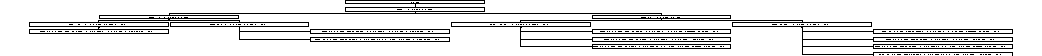
\includegraphics[height=0.936768cm]{classoomph_1_1FluidInterfaceBoundingElement}
\end{center}
\end{figure}
\subsection*{Public Member Functions}
\begin{DoxyCompactItemize}
\item 
\hyperlink{classoomph_1_1FluidInterfaceBoundingElement_ab47dc01b830d4c405002e61a7205ca7c}{Fluid\+Interface\+Bounding\+Element} ()
\begin{DoxyCompactList}\small\item\em Constructor. \end{DoxyCompactList}\item 
\hyperlink{classoomph_1_1FluidInterfaceBoundingElement_a09c0b1df7d653eaf55e94e3951d409dd}{Wall\+Unit\+Normal\+Fct\+Pt} \& \hyperlink{classoomph_1_1FluidInterfaceBoundingElement_a3d8ea7b8e1f22eaaa1235231454b753c}{wall\+\_\+unit\+\_\+normal\+\_\+fct\+\_\+pt} ()
\begin{DoxyCompactList}\small\item\em Access function\+: Pointer to wall unit normal function. \end{DoxyCompactList}\item 
\hyperlink{classoomph_1_1FluidInterfaceBoundingElement_a09c0b1df7d653eaf55e94e3951d409dd}{Wall\+Unit\+Normal\+Fct\+Pt} \hyperlink{classoomph_1_1FluidInterfaceBoundingElement_a393601b322d0b8d6d2f86d07bd17550f}{wall\+\_\+unit\+\_\+normal\+\_\+fct\+\_\+pt} () const
\begin{DoxyCompactList}\small\item\em Access function\+: Pointer to wall unit normal function. Const version. \end{DoxyCompactList}\item 
\hyperlink{classoomph_1_1Vector}{Vector}$<$ unsigned $>$ \& \hyperlink{classoomph_1_1FluidInterfaceBoundingElement_ad74aadb79a88536e188fbff44f35cc02}{u\+\_\+index\+\_\+interface\+\_\+boundary} ()
\begin{DoxyCompactList}\small\item\em Access for nodal index at which the velocity components are stored. \end{DoxyCompactList}\item 
void \hyperlink{classoomph_1_1FluidInterfaceBoundingElement_a8566c5bed5c87717fcb155d398ed8c8f}{set\+\_\+contact\+\_\+angle} (double $\ast$const \&angle\+\_\+pt, const bool \&strong=true)
\begin{DoxyCompactList}\small\item\em Set a pointer to the desired contact angle. Optional boolean (defaults to true) chooses strong imposition via hijacking (true) or weak imposition via addition to momentum equation (false). The default strong imposition is appropriate for static contact angle problems. \end{DoxyCompactList}\item 
double $\ast$\& \hyperlink{classoomph_1_1FluidInterfaceBoundingElement_a00fc3fdc8c3b7d149ba2c6de44f4a150}{contact\+\_\+angle\+\_\+pt} ()
\begin{DoxyCompactList}\small\item\em Access function to the pointer specifying the prescribed contact angle. \end{DoxyCompactList}\item 
double $\ast$\& \hyperlink{classoomph_1_1FluidInterfaceBoundingElement_acf132633ea7ed6b063c1f2a0a62d0b8c}{ca\+\_\+pt} ()
\begin{DoxyCompactList}\small\item\em Access function to the pointer specifying the capillary number. \end{DoxyCompactList}\item 
double \hyperlink{classoomph_1_1FluidInterfaceBoundingElement_ae5d097813762a2544d0b49c6e2fbaaac}{ca} ()
\begin{DoxyCompactList}\small\item\em Return the value of the capillary number. \end{DoxyCompactList}\item 
double \& \hyperlink{classoomph_1_1FluidInterfaceBoundingElement_a6803f4ea8de0b3fe17b703d7489c8147}{contact\+\_\+angle} ()
\begin{DoxyCompactList}\small\item\em Return value of the contact angle. \end{DoxyCompactList}\item 
void \hyperlink{classoomph_1_1FluidInterfaceBoundingElement_acaa709e7a402418fb03f2bf0f57f53ea}{fill\+\_\+in\+\_\+contribution\+\_\+to\+\_\+residuals} (\hyperlink{classoomph_1_1Vector}{Vector}$<$ double $>$ \&residuals)
\begin{DoxyCompactList}\small\item\em Calculate the residuals. \end{DoxyCompactList}\item 
virtual void \hyperlink{classoomph_1_1FluidInterfaceBoundingElement_a69fa099e0cbfe8ae028a4edc77fedc60}{fill\+\_\+in\+\_\+generic\+\_\+residual\+\_\+contribution\+\_\+interface\+\_\+boundary} (\hyperlink{classoomph_1_1Vector}{Vector}$<$ double $>$ \&residuals, \hyperlink{classoomph_1_1DenseMatrix}{Dense\+Matrix}$<$ double $>$ \&jacobian, unsigned flag)=0
\begin{DoxyCompactList}\small\item\em Calculate the generic residuals contribution. \end{DoxyCompactList}\item 
virtual void \hyperlink{classoomph_1_1FluidInterfaceBoundingElement_a4510bd81b572d758694715f673080041}{add\+\_\+additional\+\_\+residual\+\_\+contributions\+\_\+interface\+\_\+boundary} (\hyperlink{classoomph_1_1Vector}{Vector}$<$ double $>$ \&residuals, \hyperlink{classoomph_1_1DenseMatrix}{Dense\+Matrix}$<$ double $>$ \&jacobian, const unsigned \&flag, const \hyperlink{classoomph_1_1Shape}{Shape} \&psif, const \hyperlink{classoomph_1_1DShape}{D\+Shape} \&dpsifds, const \hyperlink{classoomph_1_1Vector}{Vector}$<$ double $>$ \&interpolated\+\_\+n, const double \&W)
\begin{DoxyCompactList}\small\item\em Empty helper function to calculate the additional contributions arising from the node update strategy to the Jacobian within the integration loop. This will be overloaded by elements that require contributions to their underlying equations from boundary integrals. The shape functions, their derivatives w.\+r.\+t. to the local coordinates, the unit normal and integral weight are passed in so that they do not have to be recalculated. \end{DoxyCompactList}\item 
void \hyperlink{classoomph_1_1FluidInterfaceBoundingElement_a81adc5ae89ddfa120f587c61b972622f}{output} (std\+::ostream \&outfile)
\begin{DoxyCompactList}\small\item\em Overload the output function. \end{DoxyCompactList}\item 
void \hyperlink{classoomph_1_1FluidInterfaceBoundingElement_af2c821d51d506221976a0c17e1615ac3}{output} (std\+::ostream \&outfile, const unsigned \&n\+\_\+plot)
\begin{DoxyCompactList}\small\item\em Output function. \end{DoxyCompactList}\item 
void \hyperlink{classoomph_1_1FluidInterfaceBoundingElement_a85cc62405429744e3e3585894315cb9e}{output} (F\+I\+LE $\ast$file\+\_\+pt)
\begin{DoxyCompactList}\small\item\em Overload the C-\/style output function. \end{DoxyCompactList}\item 
void \hyperlink{classoomph_1_1FluidInterfaceBoundingElement_ae85ea987a06275a03ad6d0e3710871da}{output} (F\+I\+LE $\ast$file\+\_\+pt, const unsigned \&n\+\_\+plot)
\begin{DoxyCompactList}\small\item\em C-\/style Output function. \end{DoxyCompactList}\end{DoxyCompactItemize}
\subsection*{Protected Member Functions}
\begin{DoxyCompactItemize}
\item 
virtual int \hyperlink{classoomph_1_1FluidInterfaceBoundingElement_a12a0a6d7c3c1c1a5a0f42a57e60eab34}{kinematic\+\_\+local\+\_\+eqn} (const unsigned \&n)=0
\begin{DoxyCompactList}\small\item\em Function that is used to determine the local equation number of the kinematic equation associated with the nodes of the element This must be overloaded depending on the node update scheme. \end{DoxyCompactList}\item 
void \hyperlink{classoomph_1_1FluidInterfaceBoundingElement_a1a715427e2037278891c06afd5d096fb}{wall\+\_\+unit\+\_\+normal} (const \hyperlink{classoomph_1_1Vector}{Vector}$<$ double $>$ \&x, \hyperlink{classoomph_1_1Vector}{Vector}$<$ double $>$ \&normal)
\begin{DoxyCompactList}\small\item\em Function that returns the unit normal of the bounding wall directed out of the fluid. \end{DoxyCompactList}\item 
void \hyperlink{classoomph_1_1FluidInterfaceBoundingElement_ab2639a1585fe815bed2d2a3d69fa5164}{update\+\_\+in\+\_\+external\+\_\+fd} (const unsigned \&\hyperlink{cfortran_8h_adb50e893b86b3e55e751a42eab3cba82}{i})
\begin{DoxyCompactList}\small\item\em The geometric data of the parent element is included as external data and so a (bulk) node update must take place after the variation of any of this external data. \end{DoxyCompactList}\item 
void \hyperlink{classoomph_1_1FluidInterfaceBoundingElement_a7347eb5984a18ffb1cfea1f9240badee}{reset\+\_\+in\+\_\+external\+\_\+fd} (const unsigned \&\hyperlink{cfortran_8h_adb50e893b86b3e55e751a42eab3cba82}{i})
\begin{DoxyCompactList}\small\item\em The only external data are these geometric data so We can omit the reset function (relying on the next update. \end{DoxyCompactList}\item 
void \hyperlink{classoomph_1_1FluidInterfaceBoundingElement_a6b0de0d11dfcfc912e2f56fbd6359ebe}{reset\+\_\+after\+\_\+external\+\_\+fd} ()
\begin{DoxyCompactList}\small\item\em We require a final node update in the bulk element after all finite differencing. \end{DoxyCompactList}\end{DoxyCompactItemize}
\subsection*{Protected Attributes}
\begin{DoxyCompactItemize}
\item 
unsigned \hyperlink{classoomph_1_1FluidInterfaceBoundingElement_affa8d787e58ca23c2e73b4c8a2c30766}{Contact\+\_\+angle\+\_\+flag}
\begin{DoxyCompactList}\small\item\em Flag used to determine whether the contact angle is to be used (0 if not), and whether it will be applied weakly as a force term in the momentum equations (1) or by hijacking the kinematic condition (2). \end{DoxyCompactList}\item 
\hyperlink{classoomph_1_1Vector}{Vector}$<$ unsigned $>$ \hyperlink{classoomph_1_1FluidInterfaceBoundingElement_a08223fefc36922f4661e30e9de16830f}{U\+\_\+index\+\_\+interface\+\_\+boundary}
\begin{DoxyCompactList}\small\item\em Index at which the i-\/th velocity component is stored in the element\textquotesingle{}s nodes. \end{DoxyCompactList}\end{DoxyCompactItemize}
\subsection*{Private Types}
\begin{DoxyCompactItemize}
\item 
typedef void($\ast$ \hyperlink{classoomph_1_1FluidInterfaceBoundingElement_a09c0b1df7d653eaf55e94e3951d409dd}{Wall\+Unit\+Normal\+Fct\+Pt}) (const \hyperlink{classoomph_1_1Vector}{Vector}$<$ double $>$ \&x, \hyperlink{classoomph_1_1Vector}{Vector}$<$ double $>$ \&unit\+\_\+normal)
\begin{DoxyCompactList}\small\item\em Function pointer to a wall unit normal function. Returns the unit normal on the wall, at the specified Eulerian coordinate. \end{DoxyCompactList}\end{DoxyCompactItemize}
\subsection*{Private Attributes}
\begin{DoxyCompactItemize}
\item 
\hyperlink{classoomph_1_1FluidInterfaceBoundingElement_a09c0b1df7d653eaf55e94e3951d409dd}{Wall\+Unit\+Normal\+Fct\+Pt} \hyperlink{classoomph_1_1FluidInterfaceBoundingElement_abc765a3b2c4eac762a1a5ba85ac4a7a4}{Wall\+\_\+unit\+\_\+normal\+\_\+fct\+\_\+pt}
\begin{DoxyCompactList}\small\item\em Pointer to a wall normal function that returns the wall unit normal as a function of position in global Eulerian coordinates. \end{DoxyCompactList}\item 
double $\ast$ \hyperlink{classoomph_1_1FluidInterfaceBoundingElement_a351532c356c9e839cba87150bea354c5}{Contact\+\_\+angle\+\_\+pt}
\begin{DoxyCompactList}\small\item\em Pointer to the desired value of the contact angle (if any) \end{DoxyCompactList}\item 
double $\ast$ \hyperlink{classoomph_1_1FluidInterfaceBoundingElement_abf47719443253c1117705b0a20e9ef70}{Ca\+\_\+pt}
\begin{DoxyCompactList}\small\item\em Pointer to the desired value of the capillary number. \end{DoxyCompactList}\end{DoxyCompactItemize}
\subsection*{Additional Inherited Members}


\subsection{Detailed Description}
Base class for elements at the boundary of free surfaces or interfaces, used typically to impose contact angle boundary conditions. The elemental dimensions are one less than those of the surface elements, or two less than those of the original bulk elements. Thus in two-\/dimensional and axi-\/symmetric problems, are points, but in three-\/dimensional problems, they are lines. These boundaries may be in contact with a solid surface, in which case the normal to that surface must be provided. 

Definition at line 58 of file interface\+\_\+elements.\+h.



\subsection{Member Typedef Documentation}
\mbox{\Hypertarget{classoomph_1_1FluidInterfaceBoundingElement_a09c0b1df7d653eaf55e94e3951d409dd}\label{classoomph_1_1FluidInterfaceBoundingElement_a09c0b1df7d653eaf55e94e3951d409dd}} 
\index{oomph\+::\+Fluid\+Interface\+Bounding\+Element@{oomph\+::\+Fluid\+Interface\+Bounding\+Element}!Wall\+Unit\+Normal\+Fct\+Pt@{Wall\+Unit\+Normal\+Fct\+Pt}}
\index{Wall\+Unit\+Normal\+Fct\+Pt@{Wall\+Unit\+Normal\+Fct\+Pt}!oomph\+::\+Fluid\+Interface\+Bounding\+Element@{oomph\+::\+Fluid\+Interface\+Bounding\+Element}}
\subsubsection{\texorpdfstring{Wall\+Unit\+Normal\+Fct\+Pt}{WallUnitNormalFctPt}}
{\footnotesize\ttfamily typedef void($\ast$ oomph\+::\+Fluid\+Interface\+Bounding\+Element\+::\+Wall\+Unit\+Normal\+Fct\+Pt) (const \hyperlink{classoomph_1_1Vector}{Vector}$<$ double $>$ \&x, \hyperlink{classoomph_1_1Vector}{Vector}$<$ double $>$ \&unit\+\_\+normal)\hspace{0.3cm}{\ttfamily [private]}}



Function pointer to a wall unit normal function. Returns the unit normal on the wall, at the specified Eulerian coordinate. 



Definition at line 64 of file interface\+\_\+elements.\+h.



\subsection{Constructor \& Destructor Documentation}
\mbox{\Hypertarget{classoomph_1_1FluidInterfaceBoundingElement_ab47dc01b830d4c405002e61a7205ca7c}\label{classoomph_1_1FluidInterfaceBoundingElement_ab47dc01b830d4c405002e61a7205ca7c}} 
\index{oomph\+::\+Fluid\+Interface\+Bounding\+Element@{oomph\+::\+Fluid\+Interface\+Bounding\+Element}!Fluid\+Interface\+Bounding\+Element@{Fluid\+Interface\+Bounding\+Element}}
\index{Fluid\+Interface\+Bounding\+Element@{Fluid\+Interface\+Bounding\+Element}!oomph\+::\+Fluid\+Interface\+Bounding\+Element@{oomph\+::\+Fluid\+Interface\+Bounding\+Element}}
\subsubsection{\texorpdfstring{Fluid\+Interface\+Bounding\+Element()}{FluidInterfaceBoundingElement()}}
{\footnotesize\ttfamily oomph\+::\+Fluid\+Interface\+Bounding\+Element\+::\+Fluid\+Interface\+Bounding\+Element (\begin{DoxyParamCaption}{ }\end{DoxyParamCaption})\hspace{0.3cm}{\ttfamily [inline]}}



Constructor. 



Definition at line 141 of file interface\+\_\+elements.\+h.



\subsection{Member Function Documentation}
\mbox{\Hypertarget{classoomph_1_1FluidInterfaceBoundingElement_a4510bd81b572d758694715f673080041}\label{classoomph_1_1FluidInterfaceBoundingElement_a4510bd81b572d758694715f673080041}} 
\index{oomph\+::\+Fluid\+Interface\+Bounding\+Element@{oomph\+::\+Fluid\+Interface\+Bounding\+Element}!add\+\_\+additional\+\_\+residual\+\_\+contributions\+\_\+interface\+\_\+boundary@{add\+\_\+additional\+\_\+residual\+\_\+contributions\+\_\+interface\+\_\+boundary}}
\index{add\+\_\+additional\+\_\+residual\+\_\+contributions\+\_\+interface\+\_\+boundary@{add\+\_\+additional\+\_\+residual\+\_\+contributions\+\_\+interface\+\_\+boundary}!oomph\+::\+Fluid\+Interface\+Bounding\+Element@{oomph\+::\+Fluid\+Interface\+Bounding\+Element}}
\subsubsection{\texorpdfstring{add\+\_\+additional\+\_\+residual\+\_\+contributions\+\_\+interface\+\_\+boundary()}{add\_additional\_residual\_contributions\_interface\_boundary()}}
{\footnotesize\ttfamily virtual void oomph\+::\+Fluid\+Interface\+Bounding\+Element\+::add\+\_\+additional\+\_\+residual\+\_\+contributions\+\_\+interface\+\_\+boundary (\begin{DoxyParamCaption}\item[{\hyperlink{classoomph_1_1Vector}{Vector}$<$ double $>$ \&}]{residuals,  }\item[{\hyperlink{classoomph_1_1DenseMatrix}{Dense\+Matrix}$<$ double $>$ \&}]{jacobian,  }\item[{const unsigned \&}]{flag,  }\item[{const \hyperlink{classoomph_1_1Shape}{Shape} \&}]{psif,  }\item[{const \hyperlink{classoomph_1_1DShape}{D\+Shape} \&}]{dpsifds,  }\item[{const \hyperlink{classoomph_1_1Vector}{Vector}$<$ double $>$ \&}]{interpolated\+\_\+n,  }\item[{const double \&}]{W }\end{DoxyParamCaption})\hspace{0.3cm}{\ttfamily [inline]}, {\ttfamily [virtual]}}



Empty helper function to calculate the additional contributions arising from the node update strategy to the Jacobian within the integration loop. This will be overloaded by elements that require contributions to their underlying equations from boundary integrals. The shape functions, their derivatives w.\+r.\+t. to the local coordinates, the unit normal and integral weight are passed in so that they do not have to be recalculated. 



Definition at line 232 of file interface\+\_\+elements.\+h.



Referenced by oomph\+::\+Point\+Fluid\+Interface\+Bounding\+Element\+::fill\+\_\+in\+\_\+generic\+\_\+residual\+\_\+contribution\+\_\+interface\+\_\+boundary(), and oomph\+::\+Line\+Fluid\+Interface\+Bounding\+Element\+::fill\+\_\+in\+\_\+generic\+\_\+residual\+\_\+contribution\+\_\+interface\+\_\+boundary().

\mbox{\Hypertarget{classoomph_1_1FluidInterfaceBoundingElement_ae5d097813762a2544d0b49c6e2fbaaac}\label{classoomph_1_1FluidInterfaceBoundingElement_ae5d097813762a2544d0b49c6e2fbaaac}} 
\index{oomph\+::\+Fluid\+Interface\+Bounding\+Element@{oomph\+::\+Fluid\+Interface\+Bounding\+Element}!ca@{ca}}
\index{ca@{ca}!oomph\+::\+Fluid\+Interface\+Bounding\+Element@{oomph\+::\+Fluid\+Interface\+Bounding\+Element}}
\subsubsection{\texorpdfstring{ca()}{ca()}}
{\footnotesize\ttfamily double oomph\+::\+Fluid\+Interface\+Bounding\+Element\+::ca (\begin{DoxyParamCaption}{ }\end{DoxyParamCaption})\hspace{0.3cm}{\ttfamily [inline]}}



Return the value of the capillary number. 



Definition at line 174 of file interface\+\_\+elements.\+h.



References Ca\+\_\+pt.



Referenced by oomph\+::\+Fluid\+Interface\+Element\+::fill\+\_\+in\+\_\+generic\+\_\+residual\+\_\+contribution\+\_\+interface(), oomph\+::\+Point\+Fluid\+Interface\+Bounding\+Element\+::fill\+\_\+in\+\_\+generic\+\_\+residual\+\_\+contribution\+\_\+interface\+\_\+boundary(), and oomph\+::\+Line\+Fluid\+Interface\+Bounding\+Element\+::fill\+\_\+in\+\_\+generic\+\_\+residual\+\_\+contribution\+\_\+interface\+\_\+boundary().

\mbox{\Hypertarget{classoomph_1_1FluidInterfaceBoundingElement_acf132633ea7ed6b063c1f2a0a62d0b8c}\label{classoomph_1_1FluidInterfaceBoundingElement_acf132633ea7ed6b063c1f2a0a62d0b8c}} 
\index{oomph\+::\+Fluid\+Interface\+Bounding\+Element@{oomph\+::\+Fluid\+Interface\+Bounding\+Element}!ca\+\_\+pt@{ca\+\_\+pt}}
\index{ca\+\_\+pt@{ca\+\_\+pt}!oomph\+::\+Fluid\+Interface\+Bounding\+Element@{oomph\+::\+Fluid\+Interface\+Bounding\+Element}}
\subsubsection{\texorpdfstring{ca\+\_\+pt()}{ca\_pt()}}
{\footnotesize\ttfamily double$\ast$ \& oomph\+::\+Fluid\+Interface\+Bounding\+Element\+::ca\+\_\+pt (\begin{DoxyParamCaption}{ }\end{DoxyParamCaption})\hspace{0.3cm}{\ttfamily [inline]}}



Access function to the pointer specifying the capillary number. 



Definition at line 171 of file interface\+\_\+elements.\+h.



References Ca\+\_\+pt.

\mbox{\Hypertarget{classoomph_1_1FluidInterfaceBoundingElement_a6803f4ea8de0b3fe17b703d7489c8147}\label{classoomph_1_1FluidInterfaceBoundingElement_a6803f4ea8de0b3fe17b703d7489c8147}} 
\index{oomph\+::\+Fluid\+Interface\+Bounding\+Element@{oomph\+::\+Fluid\+Interface\+Bounding\+Element}!contact\+\_\+angle@{contact\+\_\+angle}}
\index{contact\+\_\+angle@{contact\+\_\+angle}!oomph\+::\+Fluid\+Interface\+Bounding\+Element@{oomph\+::\+Fluid\+Interface\+Bounding\+Element}}
\subsubsection{\texorpdfstring{contact\+\_\+angle()}{contact\_angle()}}
{\footnotesize\ttfamily double\& oomph\+::\+Fluid\+Interface\+Bounding\+Element\+::contact\+\_\+angle (\begin{DoxyParamCaption}{ }\end{DoxyParamCaption})\hspace{0.3cm}{\ttfamily [inline]}}



Return value of the contact angle. 



Definition at line 195 of file interface\+\_\+elements.\+h.



References Contact\+\_\+angle\+\_\+pt, and oomph\+::\+Global\+\_\+string\+\_\+for\+\_\+annotation\+::string().



Referenced by oomph\+::\+Point\+Fluid\+Interface\+Bounding\+Element\+::fill\+\_\+in\+\_\+generic\+\_\+residual\+\_\+contribution\+\_\+interface\+\_\+boundary(), and oomph\+::\+Line\+Fluid\+Interface\+Bounding\+Element\+::fill\+\_\+in\+\_\+generic\+\_\+residual\+\_\+contribution\+\_\+interface\+\_\+boundary().

\mbox{\Hypertarget{classoomph_1_1FluidInterfaceBoundingElement_a00fc3fdc8c3b7d149ba2c6de44f4a150}\label{classoomph_1_1FluidInterfaceBoundingElement_a00fc3fdc8c3b7d149ba2c6de44f4a150}} 
\index{oomph\+::\+Fluid\+Interface\+Bounding\+Element@{oomph\+::\+Fluid\+Interface\+Bounding\+Element}!contact\+\_\+angle\+\_\+pt@{contact\+\_\+angle\+\_\+pt}}
\index{contact\+\_\+angle\+\_\+pt@{contact\+\_\+angle\+\_\+pt}!oomph\+::\+Fluid\+Interface\+Bounding\+Element@{oomph\+::\+Fluid\+Interface\+Bounding\+Element}}
\subsubsection{\texorpdfstring{contact\+\_\+angle\+\_\+pt()}{contact\_angle\_pt()}}
{\footnotesize\ttfamily double$\ast$\& oomph\+::\+Fluid\+Interface\+Bounding\+Element\+::contact\+\_\+angle\+\_\+pt (\begin{DoxyParamCaption}{ }\end{DoxyParamCaption})\hspace{0.3cm}{\ttfamily [inline]}}



Access function to the pointer specifying the prescribed contact angle. 



Definition at line 168 of file interface\+\_\+elements.\+h.



References Contact\+\_\+angle\+\_\+pt.

\mbox{\Hypertarget{classoomph_1_1FluidInterfaceBoundingElement_acaa709e7a402418fb03f2bf0f57f53ea}\label{classoomph_1_1FluidInterfaceBoundingElement_acaa709e7a402418fb03f2bf0f57f53ea}} 
\index{oomph\+::\+Fluid\+Interface\+Bounding\+Element@{oomph\+::\+Fluid\+Interface\+Bounding\+Element}!fill\+\_\+in\+\_\+contribution\+\_\+to\+\_\+residuals@{fill\+\_\+in\+\_\+contribution\+\_\+to\+\_\+residuals}}
\index{fill\+\_\+in\+\_\+contribution\+\_\+to\+\_\+residuals@{fill\+\_\+in\+\_\+contribution\+\_\+to\+\_\+residuals}!oomph\+::\+Fluid\+Interface\+Bounding\+Element@{oomph\+::\+Fluid\+Interface\+Bounding\+Element}}
\subsubsection{\texorpdfstring{fill\+\_\+in\+\_\+contribution\+\_\+to\+\_\+residuals()}{fill\_in\_contribution\_to\_residuals()}}
{\footnotesize\ttfamily void oomph\+::\+Fluid\+Interface\+Bounding\+Element\+::fill\+\_\+in\+\_\+contribution\+\_\+to\+\_\+residuals (\begin{DoxyParamCaption}\item[{\hyperlink{classoomph_1_1Vector}{Vector}$<$ double $>$ \&}]{residuals }\end{DoxyParamCaption})\hspace{0.3cm}{\ttfamily [inline]}, {\ttfamily [virtual]}}



Calculate the residuals. 



Reimplemented from \hyperlink{classoomph_1_1GeneralisedElement_a310c97f515e8504a48179c0e72c550d7}{oomph\+::\+Generalised\+Element}.



Definition at line 212 of file interface\+\_\+elements.\+h.



References oomph\+::\+Generalised\+Element\+::\+Dummy\+\_\+matrix, and fill\+\_\+in\+\_\+generic\+\_\+residual\+\_\+contribution\+\_\+interface\+\_\+boundary().

\mbox{\Hypertarget{classoomph_1_1FluidInterfaceBoundingElement_a69fa099e0cbfe8ae028a4edc77fedc60}\label{classoomph_1_1FluidInterfaceBoundingElement_a69fa099e0cbfe8ae028a4edc77fedc60}} 
\index{oomph\+::\+Fluid\+Interface\+Bounding\+Element@{oomph\+::\+Fluid\+Interface\+Bounding\+Element}!fill\+\_\+in\+\_\+generic\+\_\+residual\+\_\+contribution\+\_\+interface\+\_\+boundary@{fill\+\_\+in\+\_\+generic\+\_\+residual\+\_\+contribution\+\_\+interface\+\_\+boundary}}
\index{fill\+\_\+in\+\_\+generic\+\_\+residual\+\_\+contribution\+\_\+interface\+\_\+boundary@{fill\+\_\+in\+\_\+generic\+\_\+residual\+\_\+contribution\+\_\+interface\+\_\+boundary}!oomph\+::\+Fluid\+Interface\+Bounding\+Element@{oomph\+::\+Fluid\+Interface\+Bounding\+Element}}
\subsubsection{\texorpdfstring{fill\+\_\+in\+\_\+generic\+\_\+residual\+\_\+contribution\+\_\+interface\+\_\+boundary()}{fill\_in\_generic\_residual\_contribution\_interface\_boundary()}}
{\footnotesize\ttfamily virtual void oomph\+::\+Fluid\+Interface\+Bounding\+Element\+::fill\+\_\+in\+\_\+generic\+\_\+residual\+\_\+contribution\+\_\+interface\+\_\+boundary (\begin{DoxyParamCaption}\item[{\hyperlink{classoomph_1_1Vector}{Vector}$<$ double $>$ \&}]{residuals,  }\item[{\hyperlink{classoomph_1_1DenseMatrix}{Dense\+Matrix}$<$ double $>$ \&}]{jacobian,  }\item[{unsigned}]{flag }\end{DoxyParamCaption})\hspace{0.3cm}{\ttfamily [pure virtual]}}



Calculate the generic residuals contribution. 



Implemented in \hyperlink{classoomph_1_1LineFluidInterfaceBoundingElement_aa162a09ba8dfcba4d81e6abaa7a29986}{oomph\+::\+Line\+Fluid\+Interface\+Bounding\+Element}, and \hyperlink{classoomph_1_1PointFluidInterfaceBoundingElement_aad95a7d6f4e4349ee1136e623aa69c88}{oomph\+::\+Point\+Fluid\+Interface\+Bounding\+Element}.



Referenced by fill\+\_\+in\+\_\+contribution\+\_\+to\+\_\+residuals().

\mbox{\Hypertarget{classoomph_1_1FluidInterfaceBoundingElement_a12a0a6d7c3c1c1a5a0f42a57e60eab34}\label{classoomph_1_1FluidInterfaceBoundingElement_a12a0a6d7c3c1c1a5a0f42a57e60eab34}} 
\index{oomph\+::\+Fluid\+Interface\+Bounding\+Element@{oomph\+::\+Fluid\+Interface\+Bounding\+Element}!kinematic\+\_\+local\+\_\+eqn@{kinematic\+\_\+local\+\_\+eqn}}
\index{kinematic\+\_\+local\+\_\+eqn@{kinematic\+\_\+local\+\_\+eqn}!oomph\+::\+Fluid\+Interface\+Bounding\+Element@{oomph\+::\+Fluid\+Interface\+Bounding\+Element}}
\subsubsection{\texorpdfstring{kinematic\+\_\+local\+\_\+eqn()}{kinematic\_local\_eqn()}}
{\footnotesize\ttfamily virtual int oomph\+::\+Fluid\+Interface\+Bounding\+Element\+::kinematic\+\_\+local\+\_\+eqn (\begin{DoxyParamCaption}\item[{const unsigned \&}]{n }\end{DoxyParamCaption})\hspace{0.3cm}{\ttfamily [protected]}, {\ttfamily [pure virtual]}}



Function that is used to determine the local equation number of the kinematic equation associated with the nodes of the element This must be overloaded depending on the node update scheme. 



Implemented in \hyperlink{classoomph_1_1ElasticLineFluidInterfaceBoundingElement_a0f3d4bdd756165d6a2225f5b13eac005}{oomph\+::\+Elastic\+Line\+Fluid\+Interface\+Bounding\+Element$<$ E\+L\+E\+M\+E\+N\+T $>$}, \hyperlink{classoomph_1_1ElasticPointFluidInterfaceBoundingElement_ac3d7ce3db705bee219bf56cbb0d9ba92}{oomph\+::\+Elastic\+Point\+Fluid\+Interface\+Bounding\+Element$<$ E\+L\+E\+M\+E\+N\+T $>$}, \hyperlink{classoomph_1_1SpineLineFluidInterfaceBoundingElement_a0c31dba3e151540261753679b431b04a}{oomph\+::\+Spine\+Line\+Fluid\+Interface\+Bounding\+Element$<$ E\+L\+E\+M\+E\+N\+T $>$}, and \hyperlink{classoomph_1_1SpinePointFluidInterfaceBoundingElement_a7c1c2f31b1d9f9c925889ad199a78947}{oomph\+::\+Spine\+Point\+Fluid\+Interface\+Bounding\+Element$<$ E\+L\+E\+M\+E\+N\+T $>$}.



Referenced by oomph\+::\+Fluid\+Interface\+Element\+::fill\+\_\+in\+\_\+generic\+\_\+residual\+\_\+contribution\+\_\+interface(), oomph\+::\+Point\+Fluid\+Interface\+Bounding\+Element\+::fill\+\_\+in\+\_\+generic\+\_\+residual\+\_\+contribution\+\_\+interface\+\_\+boundary(), and oomph\+::\+Line\+Fluid\+Interface\+Bounding\+Element\+::fill\+\_\+in\+\_\+generic\+\_\+residual\+\_\+contribution\+\_\+interface\+\_\+boundary().

\mbox{\Hypertarget{classoomph_1_1FluidInterfaceBoundingElement_a81adc5ae89ddfa120f587c61b972622f}\label{classoomph_1_1FluidInterfaceBoundingElement_a81adc5ae89ddfa120f587c61b972622f}} 
\index{oomph\+::\+Fluid\+Interface\+Bounding\+Element@{oomph\+::\+Fluid\+Interface\+Bounding\+Element}!output@{output}}
\index{output@{output}!oomph\+::\+Fluid\+Interface\+Bounding\+Element@{oomph\+::\+Fluid\+Interface\+Bounding\+Element}}
\subsubsection{\texorpdfstring{output()}{output()}\hspace{0.1cm}{\footnotesize\ttfamily [1/4]}}
{\footnotesize\ttfamily void oomph\+::\+Fluid\+Interface\+Bounding\+Element\+::output (\begin{DoxyParamCaption}\item[{std\+::ostream \&}]{outfile }\end{DoxyParamCaption})\hspace{0.3cm}{\ttfamily [inline]}, {\ttfamily [virtual]}}



Overload the output function. 



Reimplemented from \hyperlink{classoomph_1_1FiniteElement_a2ad98a3d2ef4999f1bef62c0ff13f2a7}{oomph\+::\+Finite\+Element}.



Reimplemented in \hyperlink{classoomph_1_1ElasticLineFluidInterfaceBoundingElement_a50444fef924185e8d462238045e24543}{oomph\+::\+Elastic\+Line\+Fluid\+Interface\+Bounding\+Element$<$ E\+L\+E\+M\+E\+N\+T $>$}, \hyperlink{classoomph_1_1ElasticPointFluidInterfaceBoundingElement_a3a09e94ba3bf5ce0922bc4b75097078c}{oomph\+::\+Elastic\+Point\+Fluid\+Interface\+Bounding\+Element$<$ E\+L\+E\+M\+E\+N\+T $>$}, \hyperlink{classoomph_1_1SpineLineFluidInterfaceBoundingElement_a5c074690d693fa7fb349b22e926064b4}{oomph\+::\+Spine\+Line\+Fluid\+Interface\+Bounding\+Element$<$ E\+L\+E\+M\+E\+N\+T $>$}, and \hyperlink{classoomph_1_1SpinePointFluidInterfaceBoundingElement_ac35833173407cde9359c8163a0eba35c}{oomph\+::\+Spine\+Point\+Fluid\+Interface\+Bounding\+Element$<$ E\+L\+E\+M\+E\+N\+T $>$}.



Definition at line 242 of file interface\+\_\+elements.\+h.



References oomph\+::\+Finite\+Element\+::output().



Referenced by oomph\+::\+Spine\+Point\+Fluid\+Interface\+Bounding\+Element$<$ E\+L\+E\+M\+E\+N\+T $>$\+::output(), oomph\+::\+Spine\+Line\+Fluid\+Interface\+Bounding\+Element$<$ E\+L\+E\+M\+E\+N\+T $>$\+::output(), oomph\+::\+Fluid\+Interface\+Element\+::output(), oomph\+::\+Elastic\+Point\+Fluid\+Interface\+Bounding\+Element$<$ E\+L\+E\+M\+E\+N\+T $>$\+::output(), and oomph\+::\+Elastic\+Line\+Fluid\+Interface\+Bounding\+Element$<$ E\+L\+E\+M\+E\+N\+T $>$\+::output().

\mbox{\Hypertarget{classoomph_1_1FluidInterfaceBoundingElement_af2c821d51d506221976a0c17e1615ac3}\label{classoomph_1_1FluidInterfaceBoundingElement_af2c821d51d506221976a0c17e1615ac3}} 
\index{oomph\+::\+Fluid\+Interface\+Bounding\+Element@{oomph\+::\+Fluid\+Interface\+Bounding\+Element}!output@{output}}
\index{output@{output}!oomph\+::\+Fluid\+Interface\+Bounding\+Element@{oomph\+::\+Fluid\+Interface\+Bounding\+Element}}
\subsubsection{\texorpdfstring{output()}{output()}\hspace{0.1cm}{\footnotesize\ttfamily [2/4]}}
{\footnotesize\ttfamily void oomph\+::\+Fluid\+Interface\+Bounding\+Element\+::output (\begin{DoxyParamCaption}\item[{std\+::ostream \&}]{outfile,  }\item[{const unsigned \&}]{n\+\_\+plot }\end{DoxyParamCaption})\hspace{0.3cm}{\ttfamily [inline]}, {\ttfamily [virtual]}}



Output function. 



Reimplemented from \hyperlink{classoomph_1_1FiniteElement_afa9d9b2670f999b43e6679c9dd28c457}{oomph\+::\+Finite\+Element}.



Reimplemented in \hyperlink{classoomph_1_1ElasticLineFluidInterfaceBoundingElement_a7a0df1419f28df0351ed1c5e05f8f751}{oomph\+::\+Elastic\+Line\+Fluid\+Interface\+Bounding\+Element$<$ E\+L\+E\+M\+E\+N\+T $>$}, \hyperlink{classoomph_1_1ElasticPointFluidInterfaceBoundingElement_a20c0678a9fdd6ef91fe48aa1b9209c38}{oomph\+::\+Elastic\+Point\+Fluid\+Interface\+Bounding\+Element$<$ E\+L\+E\+M\+E\+N\+T $>$}, \hyperlink{classoomph_1_1SpineLineFluidInterfaceBoundingElement_a77acf17ce730f50acd0d850e7460fc4d}{oomph\+::\+Spine\+Line\+Fluid\+Interface\+Bounding\+Element$<$ E\+L\+E\+M\+E\+N\+T $>$}, and \hyperlink{classoomph_1_1SpinePointFluidInterfaceBoundingElement_a05a5383f07c840e07d8c2279cce80aaa}{oomph\+::\+Spine\+Point\+Fluid\+Interface\+Bounding\+Element$<$ E\+L\+E\+M\+E\+N\+T $>$}.



Definition at line 245 of file interface\+\_\+elements.\+h.



References oomph\+::\+Finite\+Element\+::output().

\mbox{\Hypertarget{classoomph_1_1FluidInterfaceBoundingElement_a85cc62405429744e3e3585894315cb9e}\label{classoomph_1_1FluidInterfaceBoundingElement_a85cc62405429744e3e3585894315cb9e}} 
\index{oomph\+::\+Fluid\+Interface\+Bounding\+Element@{oomph\+::\+Fluid\+Interface\+Bounding\+Element}!output@{output}}
\index{output@{output}!oomph\+::\+Fluid\+Interface\+Bounding\+Element@{oomph\+::\+Fluid\+Interface\+Bounding\+Element}}
\subsubsection{\texorpdfstring{output()}{output()}\hspace{0.1cm}{\footnotesize\ttfamily [3/4]}}
{\footnotesize\ttfamily void oomph\+::\+Fluid\+Interface\+Bounding\+Element\+::output (\begin{DoxyParamCaption}\item[{F\+I\+LE $\ast$}]{file\+\_\+pt }\end{DoxyParamCaption})\hspace{0.3cm}{\ttfamily [inline]}, {\ttfamily [virtual]}}



Overload the C-\/style output function. 



Reimplemented from \hyperlink{classoomph_1_1FiniteElement_a72cddd09f8ddbee1a20a1ff404c6943e}{oomph\+::\+Finite\+Element}.



Reimplemented in \hyperlink{classoomph_1_1ElasticLineFluidInterfaceBoundingElement_a0979784b94ab8285a964ab14077b8320}{oomph\+::\+Elastic\+Line\+Fluid\+Interface\+Bounding\+Element$<$ E\+L\+E\+M\+E\+N\+T $>$}, \hyperlink{classoomph_1_1ElasticPointFluidInterfaceBoundingElement_a61782633205934c9af1aead51640e220}{oomph\+::\+Elastic\+Point\+Fluid\+Interface\+Bounding\+Element$<$ E\+L\+E\+M\+E\+N\+T $>$}, \hyperlink{classoomph_1_1SpineLineFluidInterfaceBoundingElement_ab34fbdcd7785ab6a731a3b5d50896829}{oomph\+::\+Spine\+Line\+Fluid\+Interface\+Bounding\+Element$<$ E\+L\+E\+M\+E\+N\+T $>$}, and \hyperlink{classoomph_1_1SpinePointFluidInterfaceBoundingElement_a2435b4b786ede183808834b4d0c5210c}{oomph\+::\+Spine\+Point\+Fluid\+Interface\+Bounding\+Element$<$ E\+L\+E\+M\+E\+N\+T $>$}.



Definition at line 249 of file interface\+\_\+elements.\+h.



References oomph\+::\+Finite\+Element\+::output().

\mbox{\Hypertarget{classoomph_1_1FluidInterfaceBoundingElement_ae85ea987a06275a03ad6d0e3710871da}\label{classoomph_1_1FluidInterfaceBoundingElement_ae85ea987a06275a03ad6d0e3710871da}} 
\index{oomph\+::\+Fluid\+Interface\+Bounding\+Element@{oomph\+::\+Fluid\+Interface\+Bounding\+Element}!output@{output}}
\index{output@{output}!oomph\+::\+Fluid\+Interface\+Bounding\+Element@{oomph\+::\+Fluid\+Interface\+Bounding\+Element}}
\subsubsection{\texorpdfstring{output()}{output()}\hspace{0.1cm}{\footnotesize\ttfamily [4/4]}}
{\footnotesize\ttfamily void oomph\+::\+Fluid\+Interface\+Bounding\+Element\+::output (\begin{DoxyParamCaption}\item[{F\+I\+LE $\ast$}]{file\+\_\+pt,  }\item[{const unsigned \&}]{n\+\_\+plot }\end{DoxyParamCaption})\hspace{0.3cm}{\ttfamily [inline]}, {\ttfamily [virtual]}}



C-\/style Output function. 



Reimplemented from \hyperlink{classoomph_1_1FiniteElement_adfaee690bb0608f03320eeb9d110d48c}{oomph\+::\+Finite\+Element}.



Reimplemented in \hyperlink{classoomph_1_1ElasticLineFluidInterfaceBoundingElement_a6e4c4d356c7d66f6b5ec4c7a375ecc91}{oomph\+::\+Elastic\+Line\+Fluid\+Interface\+Bounding\+Element$<$ E\+L\+E\+M\+E\+N\+T $>$}, \hyperlink{classoomph_1_1ElasticPointFluidInterfaceBoundingElement_a4b30d56cc1869b5c9c4819843fb65ecc}{oomph\+::\+Elastic\+Point\+Fluid\+Interface\+Bounding\+Element$<$ E\+L\+E\+M\+E\+N\+T $>$}, \hyperlink{classoomph_1_1SpineLineFluidInterfaceBoundingElement_ab1dbf8b8c22f78d08d431e06db80793a}{oomph\+::\+Spine\+Line\+Fluid\+Interface\+Bounding\+Element$<$ E\+L\+E\+M\+E\+N\+T $>$}, and \hyperlink{classoomph_1_1SpinePointFluidInterfaceBoundingElement_a75a530620bfa2a983fec2e1c7f801db2}{oomph\+::\+Spine\+Point\+Fluid\+Interface\+Bounding\+Element$<$ E\+L\+E\+M\+E\+N\+T $>$}.



Definition at line 252 of file interface\+\_\+elements.\+h.



References oomph\+::\+Finite\+Element\+::output().

\mbox{\Hypertarget{classoomph_1_1FluidInterfaceBoundingElement_a6b0de0d11dfcfc912e2f56fbd6359ebe}\label{classoomph_1_1FluidInterfaceBoundingElement_a6b0de0d11dfcfc912e2f56fbd6359ebe}} 
\index{oomph\+::\+Fluid\+Interface\+Bounding\+Element@{oomph\+::\+Fluid\+Interface\+Bounding\+Element}!reset\+\_\+after\+\_\+external\+\_\+fd@{reset\+\_\+after\+\_\+external\+\_\+fd}}
\index{reset\+\_\+after\+\_\+external\+\_\+fd@{reset\+\_\+after\+\_\+external\+\_\+fd}!oomph\+::\+Fluid\+Interface\+Bounding\+Element@{oomph\+::\+Fluid\+Interface\+Bounding\+Element}}
\subsubsection{\texorpdfstring{reset\+\_\+after\+\_\+external\+\_\+fd()}{reset\_after\_external\_fd()}}
{\footnotesize\ttfamily void oomph\+::\+Fluid\+Interface\+Bounding\+Element\+::reset\+\_\+after\+\_\+external\+\_\+fd (\begin{DoxyParamCaption}{ }\end{DoxyParamCaption})\hspace{0.3cm}{\ttfamily [inline]}, {\ttfamily [protected]}, {\ttfamily [virtual]}}



We require a final node update in the bulk element after all finite differencing. 



Reimplemented from \hyperlink{classoomph_1_1GeneralisedElement_a10210277ae4fa66b7701ff00d4dd9b14}{oomph\+::\+Generalised\+Element}.



Definition at line 132 of file interface\+\_\+elements.\+h.



References oomph\+::\+Face\+Element\+::bulk\+\_\+element\+\_\+pt(), and oomph\+::\+Finite\+Element\+::node\+\_\+update().

\mbox{\Hypertarget{classoomph_1_1FluidInterfaceBoundingElement_a7347eb5984a18ffb1cfea1f9240badee}\label{classoomph_1_1FluidInterfaceBoundingElement_a7347eb5984a18ffb1cfea1f9240badee}} 
\index{oomph\+::\+Fluid\+Interface\+Bounding\+Element@{oomph\+::\+Fluid\+Interface\+Bounding\+Element}!reset\+\_\+in\+\_\+external\+\_\+fd@{reset\+\_\+in\+\_\+external\+\_\+fd}}
\index{reset\+\_\+in\+\_\+external\+\_\+fd@{reset\+\_\+in\+\_\+external\+\_\+fd}!oomph\+::\+Fluid\+Interface\+Bounding\+Element@{oomph\+::\+Fluid\+Interface\+Bounding\+Element}}
\subsubsection{\texorpdfstring{reset\+\_\+in\+\_\+external\+\_\+fd()}{reset\_in\_external\_fd()}}
{\footnotesize\ttfamily void oomph\+::\+Fluid\+Interface\+Bounding\+Element\+::reset\+\_\+in\+\_\+external\+\_\+fd (\begin{DoxyParamCaption}\item[{const unsigned \&}]{i }\end{DoxyParamCaption})\hspace{0.3cm}{\ttfamily [inline]}, {\ttfamily [protected]}, {\ttfamily [virtual]}}



The only external data are these geometric data so We can omit the reset function (relying on the next update. 



Reimplemented from \hyperlink{classoomph_1_1GeneralisedElement_a027a9213e91b946346062adf96e26a85}{oomph\+::\+Generalised\+Element}.



Definition at line 128 of file interface\+\_\+elements.\+h.

\mbox{\Hypertarget{classoomph_1_1FluidInterfaceBoundingElement_a8566c5bed5c87717fcb155d398ed8c8f}\label{classoomph_1_1FluidInterfaceBoundingElement_a8566c5bed5c87717fcb155d398ed8c8f}} 
\index{oomph\+::\+Fluid\+Interface\+Bounding\+Element@{oomph\+::\+Fluid\+Interface\+Bounding\+Element}!set\+\_\+contact\+\_\+angle@{set\+\_\+contact\+\_\+angle}}
\index{set\+\_\+contact\+\_\+angle@{set\+\_\+contact\+\_\+angle}!oomph\+::\+Fluid\+Interface\+Bounding\+Element@{oomph\+::\+Fluid\+Interface\+Bounding\+Element}}
\subsubsection{\texorpdfstring{set\+\_\+contact\+\_\+angle()}{set\_contact\_angle()}}
{\footnotesize\ttfamily void oomph\+::\+Fluid\+Interface\+Bounding\+Element\+::set\+\_\+contact\+\_\+angle (\begin{DoxyParamCaption}\item[{double $\ast$const \&}]{angle\+\_\+pt,  }\item[{const bool \&}]{strong = {\ttfamily true} }\end{DoxyParamCaption})}



Set a pointer to the desired contact angle. Optional boolean (defaults to true) chooses strong imposition via hijacking (true) or weak imposition via addition to momentum equation (false). The default strong imposition is appropriate for static contact angle problems. 

Set a pointer to the desired contact angle. Optional boolean (defaults to true) chooses strong imposition via hijacking (true) or weak imposition via addition to momentum equation (false). The default strong imposition is appropriate for static contact problems. 

Definition at line 52 of file interface\+\_\+elements.\+cc.



References oomph\+::\+Face\+Element\+::bulk\+\_\+element\+\_\+pt(), oomph\+::\+Face\+Element\+::\+Bulk\+\_\+node\+\_\+number, Contact\+\_\+angle\+\_\+flag, Contact\+\_\+angle\+\_\+pt, and oomph\+::\+Point\+Fluid\+Interface\+Bounding\+Element\+::fill\+\_\+in\+\_\+generic\+\_\+residual\+\_\+contribution\+\_\+interface\+\_\+boundary().



Referenced by u\+\_\+index\+\_\+interface\+\_\+boundary().

\mbox{\Hypertarget{classoomph_1_1FluidInterfaceBoundingElement_ad74aadb79a88536e188fbff44f35cc02}\label{classoomph_1_1FluidInterfaceBoundingElement_ad74aadb79a88536e188fbff44f35cc02}} 
\index{oomph\+::\+Fluid\+Interface\+Bounding\+Element@{oomph\+::\+Fluid\+Interface\+Bounding\+Element}!u\+\_\+index\+\_\+interface\+\_\+boundary@{u\+\_\+index\+\_\+interface\+\_\+boundary}}
\index{u\+\_\+index\+\_\+interface\+\_\+boundary@{u\+\_\+index\+\_\+interface\+\_\+boundary}!oomph\+::\+Fluid\+Interface\+Bounding\+Element@{oomph\+::\+Fluid\+Interface\+Bounding\+Element}}
\subsubsection{\texorpdfstring{u\+\_\+index\+\_\+interface\+\_\+boundary()}{u\_index\_interface\_boundary()}}
{\footnotesize\ttfamily \hyperlink{classoomph_1_1Vector}{Vector}$<$unsigned$>$\& oomph\+::\+Fluid\+Interface\+Bounding\+Element\+::u\+\_\+index\+\_\+interface\+\_\+boundary (\begin{DoxyParamCaption}{ }\end{DoxyParamCaption})\hspace{0.3cm}{\ttfamily [inline]}}



Access for nodal index at which the velocity components are stored. 



Definition at line 154 of file interface\+\_\+elements.\+h.



References set\+\_\+contact\+\_\+angle(), and U\+\_\+index\+\_\+interface\+\_\+boundary.

\mbox{\Hypertarget{classoomph_1_1FluidInterfaceBoundingElement_ab2639a1585fe815bed2d2a3d69fa5164}\label{classoomph_1_1FluidInterfaceBoundingElement_ab2639a1585fe815bed2d2a3d69fa5164}} 
\index{oomph\+::\+Fluid\+Interface\+Bounding\+Element@{oomph\+::\+Fluid\+Interface\+Bounding\+Element}!update\+\_\+in\+\_\+external\+\_\+fd@{update\+\_\+in\+\_\+external\+\_\+fd}}
\index{update\+\_\+in\+\_\+external\+\_\+fd@{update\+\_\+in\+\_\+external\+\_\+fd}!oomph\+::\+Fluid\+Interface\+Bounding\+Element@{oomph\+::\+Fluid\+Interface\+Bounding\+Element}}
\subsubsection{\texorpdfstring{update\+\_\+in\+\_\+external\+\_\+fd()}{update\_in\_external\_fd()}}
{\footnotesize\ttfamily void oomph\+::\+Fluid\+Interface\+Bounding\+Element\+::update\+\_\+in\+\_\+external\+\_\+fd (\begin{DoxyParamCaption}\item[{const unsigned \&}]{i }\end{DoxyParamCaption})\hspace{0.3cm}{\ttfamily [inline]}, {\ttfamily [protected]}, {\ttfamily [virtual]}}



The geometric data of the parent element is included as external data and so a (bulk) node update must take place after the variation of any of this external data. 



Reimplemented from \hyperlink{classoomph_1_1GeneralisedElement_af740b8c507dde03700cff5d196e28019}{oomph\+::\+Generalised\+Element}.



Definition at line 119 of file interface\+\_\+elements.\+h.



References oomph\+::\+Face\+Element\+::bulk\+\_\+element\+\_\+pt(), and oomph\+::\+Finite\+Element\+::node\+\_\+update().

\mbox{\Hypertarget{classoomph_1_1FluidInterfaceBoundingElement_a1a715427e2037278891c06afd5d096fb}\label{classoomph_1_1FluidInterfaceBoundingElement_a1a715427e2037278891c06afd5d096fb}} 
\index{oomph\+::\+Fluid\+Interface\+Bounding\+Element@{oomph\+::\+Fluid\+Interface\+Bounding\+Element}!wall\+\_\+unit\+\_\+normal@{wall\+\_\+unit\+\_\+normal}}
\index{wall\+\_\+unit\+\_\+normal@{wall\+\_\+unit\+\_\+normal}!oomph\+::\+Fluid\+Interface\+Bounding\+Element@{oomph\+::\+Fluid\+Interface\+Bounding\+Element}}
\subsubsection{\texorpdfstring{wall\+\_\+unit\+\_\+normal()}{wall\_unit\_normal()}}
{\footnotesize\ttfamily void oomph\+::\+Fluid\+Interface\+Bounding\+Element\+::wall\+\_\+unit\+\_\+normal (\begin{DoxyParamCaption}\item[{const \hyperlink{classoomph_1_1Vector}{Vector}$<$ double $>$ \&}]{x,  }\item[{\hyperlink{classoomph_1_1Vector}{Vector}$<$ double $>$ \&}]{normal }\end{DoxyParamCaption})\hspace{0.3cm}{\ttfamily [inline]}, {\ttfamily [protected]}}



Function that returns the unit normal of the bounding wall directed out of the fluid. 



Definition at line 97 of file interface\+\_\+elements.\+h.



Referenced by oomph\+::\+Point\+Fluid\+Interface\+Bounding\+Element\+::fill\+\_\+in\+\_\+generic\+\_\+residual\+\_\+contribution\+\_\+interface\+\_\+boundary(), and oomph\+::\+Line\+Fluid\+Interface\+Bounding\+Element\+::fill\+\_\+in\+\_\+generic\+\_\+residual\+\_\+contribution\+\_\+interface\+\_\+boundary().

\mbox{\Hypertarget{classoomph_1_1FluidInterfaceBoundingElement_a3d8ea7b8e1f22eaaa1235231454b753c}\label{classoomph_1_1FluidInterfaceBoundingElement_a3d8ea7b8e1f22eaaa1235231454b753c}} 
\index{oomph\+::\+Fluid\+Interface\+Bounding\+Element@{oomph\+::\+Fluid\+Interface\+Bounding\+Element}!wall\+\_\+unit\+\_\+normal\+\_\+fct\+\_\+pt@{wall\+\_\+unit\+\_\+normal\+\_\+fct\+\_\+pt}}
\index{wall\+\_\+unit\+\_\+normal\+\_\+fct\+\_\+pt@{wall\+\_\+unit\+\_\+normal\+\_\+fct\+\_\+pt}!oomph\+::\+Fluid\+Interface\+Bounding\+Element@{oomph\+::\+Fluid\+Interface\+Bounding\+Element}}
\subsubsection{\texorpdfstring{wall\+\_\+unit\+\_\+normal\+\_\+fct\+\_\+pt()}{wall\_unit\_normal\_fct\_pt()}\hspace{0.1cm}{\footnotesize\ttfamily [1/2]}}
{\footnotesize\ttfamily \hyperlink{classoomph_1_1FluidInterfaceBoundingElement_a09c0b1df7d653eaf55e94e3951d409dd}{Wall\+Unit\+Normal\+Fct\+Pt}\& oomph\+::\+Fluid\+Interface\+Bounding\+Element\+::wall\+\_\+unit\+\_\+normal\+\_\+fct\+\_\+pt (\begin{DoxyParamCaption}{ }\end{DoxyParamCaption})\hspace{0.3cm}{\ttfamily [inline]}}



Access function\+: Pointer to wall unit normal function. 



Definition at line 146 of file interface\+\_\+elements.\+h.



References Wall\+\_\+unit\+\_\+normal\+\_\+fct\+\_\+pt.

\mbox{\Hypertarget{classoomph_1_1FluidInterfaceBoundingElement_a393601b322d0b8d6d2f86d07bd17550f}\label{classoomph_1_1FluidInterfaceBoundingElement_a393601b322d0b8d6d2f86d07bd17550f}} 
\index{oomph\+::\+Fluid\+Interface\+Bounding\+Element@{oomph\+::\+Fluid\+Interface\+Bounding\+Element}!wall\+\_\+unit\+\_\+normal\+\_\+fct\+\_\+pt@{wall\+\_\+unit\+\_\+normal\+\_\+fct\+\_\+pt}}
\index{wall\+\_\+unit\+\_\+normal\+\_\+fct\+\_\+pt@{wall\+\_\+unit\+\_\+normal\+\_\+fct\+\_\+pt}!oomph\+::\+Fluid\+Interface\+Bounding\+Element@{oomph\+::\+Fluid\+Interface\+Bounding\+Element}}
\subsubsection{\texorpdfstring{wall\+\_\+unit\+\_\+normal\+\_\+fct\+\_\+pt()}{wall\_unit\_normal\_fct\_pt()}\hspace{0.1cm}{\footnotesize\ttfamily [2/2]}}
{\footnotesize\ttfamily \hyperlink{classoomph_1_1FluidInterfaceBoundingElement_a09c0b1df7d653eaf55e94e3951d409dd}{Wall\+Unit\+Normal\+Fct\+Pt} oomph\+::\+Fluid\+Interface\+Bounding\+Element\+::wall\+\_\+unit\+\_\+normal\+\_\+fct\+\_\+pt (\begin{DoxyParamCaption}{ }\end{DoxyParamCaption}) const\hspace{0.3cm}{\ttfamily [inline]}}



Access function\+: Pointer to wall unit normal function. Const version. 



Definition at line 150 of file interface\+\_\+elements.\+h.



References Wall\+\_\+unit\+\_\+normal\+\_\+fct\+\_\+pt.



\subsection{Member Data Documentation}
\mbox{\Hypertarget{classoomph_1_1FluidInterfaceBoundingElement_abf47719443253c1117705b0a20e9ef70}\label{classoomph_1_1FluidInterfaceBoundingElement_abf47719443253c1117705b0a20e9ef70}} 
\index{oomph\+::\+Fluid\+Interface\+Bounding\+Element@{oomph\+::\+Fluid\+Interface\+Bounding\+Element}!Ca\+\_\+pt@{Ca\+\_\+pt}}
\index{Ca\+\_\+pt@{Ca\+\_\+pt}!oomph\+::\+Fluid\+Interface\+Bounding\+Element@{oomph\+::\+Fluid\+Interface\+Bounding\+Element}}
\subsubsection{\texorpdfstring{Ca\+\_\+pt}{Ca\_pt}}
{\footnotesize\ttfamily double$\ast$ oomph\+::\+Fluid\+Interface\+Bounding\+Element\+::\+Ca\+\_\+pt\hspace{0.3cm}{\ttfamily [private]}}



Pointer to the desired value of the capillary number. 



Definition at line 76 of file interface\+\_\+elements.\+h.



Referenced by ca(), oomph\+::\+Fluid\+Interface\+Element\+::ca(), ca\+\_\+pt(), and oomph\+::\+Fluid\+Interface\+Element\+::ca\+\_\+pt().

\mbox{\Hypertarget{classoomph_1_1FluidInterfaceBoundingElement_affa8d787e58ca23c2e73b4c8a2c30766}\label{classoomph_1_1FluidInterfaceBoundingElement_affa8d787e58ca23c2e73b4c8a2c30766}} 
\index{oomph\+::\+Fluid\+Interface\+Bounding\+Element@{oomph\+::\+Fluid\+Interface\+Bounding\+Element}!Contact\+\_\+angle\+\_\+flag@{Contact\+\_\+angle\+\_\+flag}}
\index{Contact\+\_\+angle\+\_\+flag@{Contact\+\_\+angle\+\_\+flag}!oomph\+::\+Fluid\+Interface\+Bounding\+Element@{oomph\+::\+Fluid\+Interface\+Bounding\+Element}}
\subsubsection{\texorpdfstring{Contact\+\_\+angle\+\_\+flag}{Contact\_angle\_flag}}
{\footnotesize\ttfamily unsigned oomph\+::\+Fluid\+Interface\+Bounding\+Element\+::\+Contact\+\_\+angle\+\_\+flag\hspace{0.3cm}{\ttfamily [protected]}}



Flag used to determine whether the contact angle is to be used (0 if not), and whether it will be applied weakly as a force term in the momentum equations (1) or by hijacking the kinematic condition (2). 



Definition at line 84 of file interface\+\_\+elements.\+h.



Referenced by oomph\+::\+Point\+Fluid\+Interface\+Bounding\+Element\+::fill\+\_\+in\+\_\+generic\+\_\+residual\+\_\+contribution\+\_\+interface\+\_\+boundary(), oomph\+::\+Line\+Fluid\+Interface\+Bounding\+Element\+::fill\+\_\+in\+\_\+generic\+\_\+residual\+\_\+contribution\+\_\+interface\+\_\+boundary(), and set\+\_\+contact\+\_\+angle().

\mbox{\Hypertarget{classoomph_1_1FluidInterfaceBoundingElement_a351532c356c9e839cba87150bea354c5}\label{classoomph_1_1FluidInterfaceBoundingElement_a351532c356c9e839cba87150bea354c5}} 
\index{oomph\+::\+Fluid\+Interface\+Bounding\+Element@{oomph\+::\+Fluid\+Interface\+Bounding\+Element}!Contact\+\_\+angle\+\_\+pt@{Contact\+\_\+angle\+\_\+pt}}
\index{Contact\+\_\+angle\+\_\+pt@{Contact\+\_\+angle\+\_\+pt}!oomph\+::\+Fluid\+Interface\+Bounding\+Element@{oomph\+::\+Fluid\+Interface\+Bounding\+Element}}
\subsubsection{\texorpdfstring{Contact\+\_\+angle\+\_\+pt}{Contact\_angle\_pt}}
{\footnotesize\ttfamily double$\ast$ oomph\+::\+Fluid\+Interface\+Bounding\+Element\+::\+Contact\+\_\+angle\+\_\+pt\hspace{0.3cm}{\ttfamily [private]}}



Pointer to the desired value of the contact angle (if any) 



Definition at line 73 of file interface\+\_\+elements.\+h.



Referenced by contact\+\_\+angle(), contact\+\_\+angle\+\_\+pt(), and set\+\_\+contact\+\_\+angle().

\mbox{\Hypertarget{classoomph_1_1FluidInterfaceBoundingElement_a08223fefc36922f4661e30e9de16830f}\label{classoomph_1_1FluidInterfaceBoundingElement_a08223fefc36922f4661e30e9de16830f}} 
\index{oomph\+::\+Fluid\+Interface\+Bounding\+Element@{oomph\+::\+Fluid\+Interface\+Bounding\+Element}!U\+\_\+index\+\_\+interface\+\_\+boundary@{U\+\_\+index\+\_\+interface\+\_\+boundary}}
\index{U\+\_\+index\+\_\+interface\+\_\+boundary@{U\+\_\+index\+\_\+interface\+\_\+boundary}!oomph\+::\+Fluid\+Interface\+Bounding\+Element@{oomph\+::\+Fluid\+Interface\+Bounding\+Element}}
\subsubsection{\texorpdfstring{U\+\_\+index\+\_\+interface\+\_\+boundary}{U\_index\_interface\_boundary}}
{\footnotesize\ttfamily \hyperlink{classoomph_1_1Vector}{Vector}$<$unsigned$>$ oomph\+::\+Fluid\+Interface\+Bounding\+Element\+::\+U\+\_\+index\+\_\+interface\+\_\+boundary\hspace{0.3cm}{\ttfamily [protected]}}



Index at which the i-\/th velocity component is stored in the element\textquotesingle{}s nodes. 



Definition at line 88 of file interface\+\_\+elements.\+h.



Referenced by oomph\+::\+Point\+Fluid\+Interface\+Bounding\+Element\+::fill\+\_\+in\+\_\+generic\+\_\+residual\+\_\+contribution\+\_\+interface\+\_\+boundary(), oomph\+::\+Line\+Fluid\+Interface\+Bounding\+Element\+::fill\+\_\+in\+\_\+generic\+\_\+residual\+\_\+contribution\+\_\+interface\+\_\+boundary(), and u\+\_\+index\+\_\+interface\+\_\+boundary().

\mbox{\Hypertarget{classoomph_1_1FluidInterfaceBoundingElement_abc765a3b2c4eac762a1a5ba85ac4a7a4}\label{classoomph_1_1FluidInterfaceBoundingElement_abc765a3b2c4eac762a1a5ba85ac4a7a4}} 
\index{oomph\+::\+Fluid\+Interface\+Bounding\+Element@{oomph\+::\+Fluid\+Interface\+Bounding\+Element}!Wall\+\_\+unit\+\_\+normal\+\_\+fct\+\_\+pt@{Wall\+\_\+unit\+\_\+normal\+\_\+fct\+\_\+pt}}
\index{Wall\+\_\+unit\+\_\+normal\+\_\+fct\+\_\+pt@{Wall\+\_\+unit\+\_\+normal\+\_\+fct\+\_\+pt}!oomph\+::\+Fluid\+Interface\+Bounding\+Element@{oomph\+::\+Fluid\+Interface\+Bounding\+Element}}
\subsubsection{\texorpdfstring{Wall\+\_\+unit\+\_\+normal\+\_\+fct\+\_\+pt}{Wall\_unit\_normal\_fct\_pt}}
{\footnotesize\ttfamily \hyperlink{classoomph_1_1FluidInterfaceBoundingElement_a09c0b1df7d653eaf55e94e3951d409dd}{Wall\+Unit\+Normal\+Fct\+Pt} oomph\+::\+Fluid\+Interface\+Bounding\+Element\+::\+Wall\+\_\+unit\+\_\+normal\+\_\+fct\+\_\+pt\hspace{0.3cm}{\ttfamily [private]}}



Pointer to a wall normal function that returns the wall unit normal as a function of position in global Eulerian coordinates. 



Definition at line 70 of file interface\+\_\+elements.\+h.



Referenced by wall\+\_\+unit\+\_\+normal\+\_\+fct\+\_\+pt().



The documentation for this class was generated from the following files\+:\begin{DoxyCompactItemize}
\item 
\hyperlink{interface__elements_8h}{interface\+\_\+elements.\+h}\item 
\hyperlink{interface__elements_8cc}{interface\+\_\+elements.\+cc}\end{DoxyCompactItemize}

\hypertarget{classoomph_1_1FluidInterfaceElement}{}\section{oomph\+:\+:Fluid\+Interface\+Element Class Reference}
\label{classoomph_1_1FluidInterfaceElement}\index{oomph\+::\+Fluid\+Interface\+Element@{oomph\+::\+Fluid\+Interface\+Element}}


{\ttfamily \#include $<$interface\+\_\+elements.\+h$>$}

Inheritance diagram for oomph\+:\+:Fluid\+Interface\+Element\+:\begin{figure}[H]
\begin{center}
\leavevmode
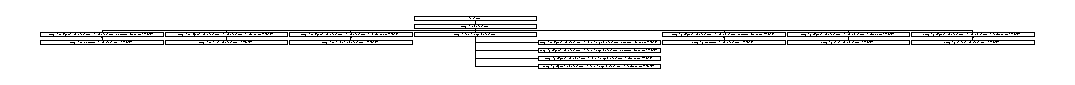
\includegraphics[height=0.695035cm]{classoomph_1_1FluidInterfaceElement}
\end{center}
\end{figure}
\subsection*{Public Member Functions}
\begin{DoxyCompactItemize}
\item 
\hyperlink{classoomph_1_1FluidInterfaceElement_a4bd4a44ee08780fb8ba1be83c4353dd4}{Fluid\+Interface\+Element} ()
\begin{DoxyCompactList}\small\item\em Constructor, set the default values of the booleans and pointers (null) \end{DoxyCompactList}\item 
virtual double \hyperlink{classoomph_1_1FluidInterfaceElement_a7e5c3ca1eba5d4dd44c0eab9be252c2a}{sigma} (const Vector$<$ double $>$ \&s\+\_\+local)
\begin{DoxyCompactList}\small\item\em Virtual function that specifies the non-\/dimensional surface tension as a function of local position within the element. The default behaviour is a constant surface tension of value 1.\+0 This function can be overloaded in more specialised elements to incorporate variations in surface tension. \end{DoxyCompactList}\item 
void \hyperlink{classoomph_1_1FluidInterfaceElement_a3f66ffd5d9a8b9b6bd8cd54e90ce2d61}{fill\+\_\+in\+\_\+contribution\+\_\+to\+\_\+residuals} (Vector$<$ double $>$ \&residuals)
\begin{DoxyCompactList}\small\item\em Calculate the residuals by calling the generic residual contribution. \end{DoxyCompactList}\item 
const double \& \hyperlink{classoomph_1_1FluidInterfaceElement_abcb18ff13b322136dd2346a6b40ecabc}{ca} () const
\begin{DoxyCompactList}\small\item\em The value of the Capillary number. \end{DoxyCompactList}\item 
double $\ast$\& \hyperlink{classoomph_1_1FluidInterfaceElement_a1a950f0202d6dd15fab2f0c03927edc9}{ca\+\_\+pt} ()
\begin{DoxyCompactList}\small\item\em Pointer to the Capillary number. \end{DoxyCompactList}\item 
const double \& \hyperlink{classoomph_1_1FluidInterfaceElement_a0c55c0e3cff597363ecb9ab0869c0015}{st} () const
\begin{DoxyCompactList}\small\item\em The value of the Strouhal number. \end{DoxyCompactList}\item 
double $\ast$\& \hyperlink{classoomph_1_1FluidInterfaceElement_a3fa462bb0ff807cf655ba02b35c1ccb4}{st\+\_\+pt} ()
\begin{DoxyCompactList}\small\item\em The pointer to the Strouhal number. \end{DoxyCompactList}\item 
double \hyperlink{classoomph_1_1FluidInterfaceElement_a50a509413ea7f2a481678837846dd476}{u} (const unsigned \&j, const unsigned \&i)
\begin{DoxyCompactList}\small\item\em Return the i-\/th velocity component at local node j. \end{DoxyCompactList}\item 
double \hyperlink{classoomph_1_1FluidInterfaceElement_a8f807a6456da7785b12e45a4c17fb969}{interpolated\+\_\+u} (const Vector$<$ double $>$ \&s, const unsigned \&i)
\begin{DoxyCompactList}\small\item\em Calculate the i-\/th velocity component at the local coordinate s. \end{DoxyCompactList}\item 
double \hyperlink{classoomph_1_1FluidInterfaceElement_a7c0a2a21afce911c301c75febd3ba44c}{pext} () const
\begin{DoxyCompactList}\small\item\em Return the value of the external pressure. \end{DoxyCompactList}\item 
void \hyperlink{classoomph_1_1FluidInterfaceElement_a7230ddea36eb36938d64583e5ee4b15f}{set\+\_\+external\+\_\+pressure\+\_\+data} (Data $\ast$external\+\_\+pressure\+\_\+data\+\_\+pt)
\begin{DoxyCompactList}\small\item\em Set the Data that contains the single pressure value that specifies the \char`\"{}external pressure\char`\"{} for the interface/free-\/surface. Setting this only makes sense if the interface is, in fact, a free surface (well, an interface to another inviscid fluid if you want to be picky). \end{DoxyCompactList}\item 
void \hyperlink{classoomph_1_1FluidInterfaceElement_a87ee1f3227c456a4c30df77c4d0bad6b}{set\+\_\+external\+\_\+pressure\+\_\+data} (Data $\ast$external\+\_\+pressure\+\_\+data\+\_\+pt, const unsigned \&index\+\_\+of\+\_\+external\+\_\+pressure\+\_\+value)
\begin{DoxyCompactList}\small\item\em Set the Data that contains the pressure value that specifies the \char`\"{}external pressure\char`\"{} for the interface/free-\/surface. Setting this only makes sense if the interface is, in fact, a free surface (well, an interface to another inviscid fluid if you want to be picky). Second argument specifies the index of the pressure value within the Data object. \end{DoxyCompactList}\item 
virtual \hyperlink{classoomph_1_1FluidInterfaceBoundingElement}{Fluid\+Interface\+Bounding\+Element} $\ast$ \hyperlink{classoomph_1_1FluidInterfaceElement_a376f8d1d451890b5725c7a991c34b6fc}{make\+\_\+bounding\+\_\+element} (const int \&face\+\_\+index)
\begin{DoxyCompactList}\small\item\em Create a bounding element e.\+g. to apply a contact angle boundary condition. \end{DoxyCompactList}\item 
virtual void \hyperlink{classoomph_1_1FluidInterfaceElement_a7eb949642baee233779e4f92478ea341}{hijack\+\_\+kinematic\+\_\+conditions} (const Vector$<$ unsigned $>$ \&bulk\+\_\+node\+\_\+number)=0
\begin{DoxyCompactList}\small\item\em Hijack the kinematic condition at the node numbers passed in the vector. The node numbers correspond to the local numbers of nodes in the associated bulk element. This is required so that contact-\/angle conditions can be applied by the Fluid\+Interface\+Bounding\+Elements. \end{DoxyCompactList}\item 
void \hyperlink{classoomph_1_1FluidInterfaceElement_aba83fbd0679ffca4ef6aa32f7aa5d179}{output} (std\+::ostream \&outfile)
\begin{DoxyCompactList}\small\item\em Overload the output function. \end{DoxyCompactList}\item 
void \hyperlink{classoomph_1_1FluidInterfaceElement_a213b1a40132a9605ee8bd31c88b225e0}{output} (std\+::ostream \&outfile, const unsigned \&n\+\_\+plot)
\begin{DoxyCompactList}\small\item\em Output function. \end{DoxyCompactList}\item 
void \hyperlink{classoomph_1_1FluidInterfaceElement_ad39bb9862c7f76e07d5ac006a1209cf9}{output} (F\+I\+LE $\ast$file\+\_\+pt)
\begin{DoxyCompactList}\small\item\em Overload the C-\/style output function. \end{DoxyCompactList}\item 
void \hyperlink{classoomph_1_1FluidInterfaceElement_a57efd66ae07fab9e0cf98ac5f8eeb000}{output} (F\+I\+LE $\ast$file\+\_\+pt, const unsigned \&n\+\_\+plot)
\begin{DoxyCompactList}\small\item\em C-\/style Output function. \end{DoxyCompactList}\end{DoxyCompactItemize}
\subsection*{Protected Member Functions}
\begin{DoxyCompactItemize}
\item 
virtual int \hyperlink{classoomph_1_1FluidInterfaceElement_a58a82e2fd839d4381e43d46a22bf1f25}{kinematic\+\_\+local\+\_\+eqn} (const unsigned \&n)=0
\begin{DoxyCompactList}\small\item\em Access function that returns the local equation number for the (scalar) kinematic equation associated with the j-\/th local node. This must be overloaded by specific interface elements and depends on the method for handing the free-\/surface deformation. \end{DoxyCompactList}\item 
int \hyperlink{classoomph_1_1FluidInterfaceElement_abd4aece98dee8173c6d796e23ccf1e03}{pext\+\_\+local\+\_\+eqn} ()
\begin{DoxyCompactList}\small\item\em Access function for the local equation number that corresponds to the external pressure. \end{DoxyCompactList}\item 
virtual void \hyperlink{classoomph_1_1FluidInterfaceElement_ae4ea3a18a513bed3725fdf413cf18874}{fill\+\_\+in\+\_\+generic\+\_\+residual\+\_\+contribution\+\_\+interface} (Vector$<$ double $>$ \&residuals, Dense\+Matrix$<$ double $>$ \&jacobian, unsigned flag)
\begin{DoxyCompactList}\small\item\em Helper function to calculate the residuals and (if flag==1) the Jacobian of the equations. This is implemented generically using the surface divergence information that is overloaded in each element i.\+e. axisymmetric, two-\/ or three-\/dimensional. \end{DoxyCompactList}\item 
virtual double \hyperlink{classoomph_1_1FluidInterfaceElement_a0180a8e36fadbbe6984f9b3c5edffc81}{compute\+\_\+surface\+\_\+derivatives} (const Shape \&psi, const D\+Shape \&dpsids, const Dense\+Matrix$<$ double $>$ \&interpolated\+\_\+t, const Vector$<$ double $>$ \&interpolated\+\_\+x, D\+Shape \&dpsidS, D\+Shape \&dpsid\+S\+\_\+div)=0
\begin{DoxyCompactList}\small\item\em Compute the surface gradient and surface divergence operators given the shape functions, derivatives, tangent vectors and position. All derivatives and tangent vectors should be formed with respect to the local coordinates. \end{DoxyCompactList}\item 
virtual void \hyperlink{classoomph_1_1FluidInterfaceElement_a0bc278bb201b861f47dc846453be4c06}{add\+\_\+additional\+\_\+residual\+\_\+contributions\+\_\+interface} (Vector$<$ double $>$ \&residuals, Dense\+Matrix$<$ double $>$ \&jacobian, const unsigned \&flag, const Shape \&psif, const D\+Shape \&dpsifds, const D\+Shape \&dpsifdS, const D\+Shape \&dpsifd\+S\+\_\+div, const Vector$<$ double $>$ \&s, const Vector$<$ double $>$ \&interpolated\+\_\+x, const Vector$<$ double $>$ \&interpolated\+\_\+n, const double \&W, const double \&J)
\begin{DoxyCompactList}\small\item\em Helper function to calculate the additional contributions to the resisuals and Jacobian that arise from specific node update strategies. This is called within the integration loop over the element (for efficiency) and therefore requires a fairly large number of input parameters\+: \end{DoxyCompactList}\end{DoxyCompactItemize}
\subsection*{Protected Attributes}
\begin{DoxyCompactItemize}
\item 
Vector$<$ unsigned $>$ \hyperlink{classoomph_1_1FluidInterfaceElement_a6a818d9999c68641223edcad217a8c3f}{U\+\_\+index\+\_\+interface}
\begin{DoxyCompactList}\small\item\em Nodal index at which the i-\/th velocity component is stored. \end{DoxyCompactList}\item 
int \hyperlink{classoomph_1_1FluidInterfaceElement_a2d4c5b3e08177f5695fa9e76bf08b570}{External\+\_\+data\+\_\+number\+\_\+of\+\_\+external\+\_\+pressure}
\begin{DoxyCompactList}\small\item\em The Data that contains the external pressure is stored as external Data for the element. Which external Data item is it? (int so it can be initialised to -\/1, indicating that external pressure hasn\textquotesingle{}t been set). \end{DoxyCompactList}\item 
Data $\ast$ \hyperlink{classoomph_1_1FluidInterfaceElement_a9177eb6e96e5ac13fe092596bc104910}{Pext\+\_\+data\+\_\+pt}
\begin{DoxyCompactList}\small\item\em Pointer to the Data item that stores the external pressure. \end{DoxyCompactList}\item 
unsigned \hyperlink{classoomph_1_1FluidInterfaceElement_a2a49c97d42ce05d1876626e5918bb8eb}{Index\+\_\+of\+\_\+external\+\_\+pressure\+\_\+value}
\begin{DoxyCompactList}\small\item\em Which of the values in Pext\+\_\+data\+\_\+pt stores the external pressure. \end{DoxyCompactList}\end{DoxyCompactItemize}
\subsection*{Private Attributes}
\begin{DoxyCompactItemize}
\item 
double $\ast$ \hyperlink{classoomph_1_1FluidInterfaceElement_adaf6e3c6739fb9081f8865773a4d0c2c}{Ca\+\_\+pt}
\begin{DoxyCompactList}\small\item\em Pointer to the Capillary number. \end{DoxyCompactList}\item 
double $\ast$ \hyperlink{classoomph_1_1FluidInterfaceElement_ae32ade5ea1742938f538e5d5f812bb2a}{St\+\_\+pt}
\begin{DoxyCompactList}\small\item\em Pointer to the Strouhal number. \end{DoxyCompactList}\end{DoxyCompactItemize}
\subsection*{Static Private Attributes}
\begin{DoxyCompactItemize}
\item 
static double \hyperlink{classoomph_1_1FluidInterfaceElement_adbe9dc951b87449522f6d19e4acac538}{Default\+\_\+\+Physical\+\_\+\+Constant\+\_\+\+Value} = 1.\+0
\begin{DoxyCompactList}\small\item\em Default value for physical constants. \end{DoxyCompactList}\end{DoxyCompactItemize}
\subsection*{Friends}
\begin{DoxyCompactItemize}
\item 
class \hyperlink{classoomph_1_1FluidInterfaceElement_af0eab9c2aa8fc5a5006df03ab93c015f}{Fluid\+Interface\+Bounding\+Element}
\end{DoxyCompactItemize}


\subsection{Detailed Description}
Base class establishing common interfaces and functions for all Navier-\/\+Stokes-\/like fluid interface elements. Namely, elements that represent either a free surface or an interface between two fluids that have distinct momentum-\/like equation for each velocity component. 

Definition at line 322 of file interface\+\_\+elements.\+h.



\subsection{Constructor \& Destructor Documentation}
\mbox{\Hypertarget{classoomph_1_1FluidInterfaceElement_a4bd4a44ee08780fb8ba1be83c4353dd4}\label{classoomph_1_1FluidInterfaceElement_a4bd4a44ee08780fb8ba1be83c4353dd4}} 
\index{oomph\+::\+Fluid\+Interface\+Element@{oomph\+::\+Fluid\+Interface\+Element}!Fluid\+Interface\+Element@{Fluid\+Interface\+Element}}
\index{Fluid\+Interface\+Element@{Fluid\+Interface\+Element}!oomph\+::\+Fluid\+Interface\+Element@{oomph\+::\+Fluid\+Interface\+Element}}
\subsubsection{\texorpdfstring{Fluid\+Interface\+Element()}{FluidInterfaceElement()}}
{\footnotesize\ttfamily oomph\+::\+Fluid\+Interface\+Element\+::\+Fluid\+Interface\+Element (\begin{DoxyParamCaption}{ }\end{DoxyParamCaption})\hspace{0.3cm}{\ttfamily [inline]}}



Constructor, set the default values of the booleans and pointers (null) 



Definition at line 448 of file interface\+\_\+elements.\+h.



\subsection{Member Function Documentation}
\mbox{\Hypertarget{classoomph_1_1FluidInterfaceElement_a0bc278bb201b861f47dc846453be4c06}\label{classoomph_1_1FluidInterfaceElement_a0bc278bb201b861f47dc846453be4c06}} 
\index{oomph\+::\+Fluid\+Interface\+Element@{oomph\+::\+Fluid\+Interface\+Element}!add\+\_\+additional\+\_\+residual\+\_\+contributions\+\_\+interface@{add\+\_\+additional\+\_\+residual\+\_\+contributions\+\_\+interface}}
\index{add\+\_\+additional\+\_\+residual\+\_\+contributions\+\_\+interface@{add\+\_\+additional\+\_\+residual\+\_\+contributions\+\_\+interface}!oomph\+::\+Fluid\+Interface\+Element@{oomph\+::\+Fluid\+Interface\+Element}}
\subsubsection{\texorpdfstring{add\+\_\+additional\+\_\+residual\+\_\+contributions\+\_\+interface()}{add\_additional\_residual\_contributions\_interface()}}
{\footnotesize\ttfamily virtual void oomph\+::\+Fluid\+Interface\+Element\+::add\+\_\+additional\+\_\+residual\+\_\+contributions\+\_\+interface (\begin{DoxyParamCaption}\item[{Vector$<$ double $>$ \&}]{residuals,  }\item[{Dense\+Matrix$<$ double $>$ \&}]{jacobian,  }\item[{const unsigned \&}]{flag,  }\item[{const Shape \&}]{psif,  }\item[{const D\+Shape \&}]{dpsifds,  }\item[{const D\+Shape \&}]{dpsifdS,  }\item[{const D\+Shape \&}]{dpsifd\+S\+\_\+div,  }\item[{const Vector$<$ double $>$ \&}]{s,  }\item[{const Vector$<$ double $>$ \&}]{interpolated\+\_\+x,  }\item[{const Vector$<$ double $>$ \&}]{interpolated\+\_\+n,  }\item[{const double \&}]{W,  }\item[{const double \&}]{J }\end{DoxyParamCaption})\hspace{0.3cm}{\ttfamily [inline]}, {\ttfamily [protected]}, {\ttfamily [virtual]}}



Helper function to calculate the additional contributions to the resisuals and Jacobian that arise from specific node update strategies. This is called within the integration loop over the element (for efficiency) and therefore requires a fairly large number of input parameters\+: 


\begin{DoxyItemize}
\item the velocity shape functions and their derivatives w.\+r.\+t. the local coordinates
\item the surface gradient and divergence of the velocity shape functions
\item The local and Eulerian coordinates,
\item the outer unit normal,
\item the integration weight from the integration scheme
\item the Jacobian of the mapping between the local and global coordinates along the element. (Note that in the axisymmmetric case this includes the r term)! 
\end{DoxyItemize}

Reimplemented in \hyperlink{classoomph_1_1ElasticUpdateFluidInterfaceElement_a15c3d2912325ace17676366c1469121f}{oomph\+::\+Elastic\+Update\+Fluid\+Interface\+Element$<$ Fluid\+Interface\+Element, Surface\+Derivatives, E\+L\+E\+M\+E\+N\+T $>$}, \hyperlink{classoomph_1_1ElasticUpdateFluidInterfaceElement_a15c3d2912325ace17676366c1469121f}{oomph\+::\+Elastic\+Update\+Fluid\+Interface\+Element$<$ Surfactant\+Transport\+Interface\+Element, Axisymmetric\+Derivatives, E\+L\+E\+M\+E\+N\+T $>$}, \hyperlink{classoomph_1_1ElasticUpdateFluidInterfaceElement_a15c3d2912325ace17676366c1469121f}{oomph\+::\+Elastic\+Update\+Fluid\+Interface\+Element$<$ Fluid\+Interface\+Element, Axisymmetric\+Derivatives, E\+L\+E\+M\+E\+N\+T $>$}, \hyperlink{classoomph_1_1ElasticUpdateFluidInterfaceElement_a15c3d2912325ace17676366c1469121f}{oomph\+::\+Elastic\+Update\+Fluid\+Interface\+Element$<$ Fluid\+Interface\+Element, Line\+Derivatives, E\+L\+E\+M\+E\+N\+T $>$}, \hyperlink{classoomph_1_1SpineAxisymmetricMarangoniSurfactantFluidInterfaceElement_a56c90572b8969dff01a4baa9de850d91}{oomph\+::\+Spine\+Axisymmetric\+Marangoni\+Surfactant\+Fluid\+Interface\+Element$<$ E\+L\+E\+M\+E\+N\+T $>$}, \hyperlink{classoomph_1_1SpineUpdateFluidInterfaceElement_a3958845051cafecd8e73745fc04c7a78}{oomph\+::\+Spine\+Update\+Fluid\+Interface\+Element$<$ Surfactant\+Transport\+Interface\+Element, Line\+Derivatives, E\+L\+E\+M\+E\+N\+T $>$}, \hyperlink{classoomph_1_1SpineUpdateFluidInterfaceElement_a3958845051cafecd8e73745fc04c7a78}{oomph\+::\+Spine\+Update\+Fluid\+Interface\+Element$<$ Fluid\+Interface\+Element, Surface\+Derivatives, E\+L\+E\+M\+E\+N\+T $>$}, \hyperlink{classoomph_1_1SpineUpdateFluidInterfaceElement_a3958845051cafecd8e73745fc04c7a78}{oomph\+::\+Spine\+Update\+Fluid\+Interface\+Element$<$ Surfactant\+Transport\+Interface\+Element, Axisymmetric\+Derivatives, E\+L\+E\+M\+E\+N\+T $>$}, \hyperlink{classoomph_1_1SpineUpdateFluidInterfaceElement_a3958845051cafecd8e73745fc04c7a78}{oomph\+::\+Spine\+Update\+Fluid\+Interface\+Element$<$ Surfactant\+Transport\+Interface\+Element, Surface\+Derivatives, E\+L\+E\+M\+E\+N\+T $>$}, \hyperlink{classoomph_1_1SpineUpdateFluidInterfaceElement_a3958845051cafecd8e73745fc04c7a78}{oomph\+::\+Spine\+Update\+Fluid\+Interface\+Element$<$ Fluid\+Interface\+Element, Axisymmetric\+Derivatives, E\+L\+E\+M\+E\+N\+T $>$}, \hyperlink{classoomph_1_1SpineUpdateFluidInterfaceElement_a3958845051cafecd8e73745fc04c7a78}{oomph\+::\+Spine\+Update\+Fluid\+Interface\+Element$<$ Fluid\+Interface\+Element, Line\+Derivatives, E\+L\+E\+M\+E\+N\+T $>$}, \hyperlink{classElasticAxisymmetricSolubleSurfactantTransportInterfaceElement_a054c0dfcc88814e128318c7ad30e6e31}{Elastic\+Axisymmetric\+Soluble\+Surfactant\+Transport\+Interface\+Element$<$ E\+L\+E\+M\+E\+N\+T $>$}, and \hyperlink{classoomph_1_1SurfactantTransportInterfaceElement_adedf33390efdf652e169f8bd38eb2350}{oomph\+::\+Surfactant\+Transport\+Interface\+Element}.



Definition at line 430 of file interface\+\_\+elements.\+h.

\mbox{\Hypertarget{classoomph_1_1FluidInterfaceElement_abcb18ff13b322136dd2346a6b40ecabc}\label{classoomph_1_1FluidInterfaceElement_abcb18ff13b322136dd2346a6b40ecabc}} 
\index{oomph\+::\+Fluid\+Interface\+Element@{oomph\+::\+Fluid\+Interface\+Element}!ca@{ca}}
\index{ca@{ca}!oomph\+::\+Fluid\+Interface\+Element@{oomph\+::\+Fluid\+Interface\+Element}}
\subsubsection{\texorpdfstring{ca()}{ca()}}
{\footnotesize\ttfamily const double\& oomph\+::\+Fluid\+Interface\+Element\+::ca (\begin{DoxyParamCaption}{ }\end{DoxyParamCaption}) const\hspace{0.3cm}{\ttfamily [inline]}}



The value of the Capillary number. 



Definition at line 475 of file interface\+\_\+elements.\+h.



References oomph\+::\+Fluid\+Interface\+Bounding\+Element\+::\+Ca\+\_\+pt.



Referenced by oomph\+::\+Surfactant\+Transport\+Interface\+Element\+::add\+\_\+additional\+\_\+residual\+\_\+contributions\+\_\+interface().

\mbox{\Hypertarget{classoomph_1_1FluidInterfaceElement_a1a950f0202d6dd15fab2f0c03927edc9}\label{classoomph_1_1FluidInterfaceElement_a1a950f0202d6dd15fab2f0c03927edc9}} 
\index{oomph\+::\+Fluid\+Interface\+Element@{oomph\+::\+Fluid\+Interface\+Element}!ca\+\_\+pt@{ca\+\_\+pt}}
\index{ca\+\_\+pt@{ca\+\_\+pt}!oomph\+::\+Fluid\+Interface\+Element@{oomph\+::\+Fluid\+Interface\+Element}}
\subsubsection{\texorpdfstring{ca\+\_\+pt()}{ca\_pt()}}
{\footnotesize\ttfamily double$\ast$\& oomph\+::\+Fluid\+Interface\+Element\+::ca\+\_\+pt (\begin{DoxyParamCaption}{ }\end{DoxyParamCaption})\hspace{0.3cm}{\ttfamily [inline]}}



Pointer to the Capillary number. 



Definition at line 494 of file interface\+\_\+elements.\+h.



References oomph\+::\+Fluid\+Interface\+Bounding\+Element\+::\+Ca\+\_\+pt.



Referenced by Interface\+Problem$<$ E\+L\+E\+M\+E\+N\+T, T\+I\+M\+E\+S\+T\+E\+P\+P\+E\+R $>$\+::deform\+\_\+free\+\_\+surface(), and Interface\+Problem$<$ E\+L\+E\+M\+E\+N\+T, T\+I\+M\+E\+S\+T\+E\+P\+P\+E\+R $>$\+::\+Interface\+Problem().

\mbox{\Hypertarget{classoomph_1_1FluidInterfaceElement_a0180a8e36fadbbe6984f9b3c5edffc81}\label{classoomph_1_1FluidInterfaceElement_a0180a8e36fadbbe6984f9b3c5edffc81}} 
\index{oomph\+::\+Fluid\+Interface\+Element@{oomph\+::\+Fluid\+Interface\+Element}!compute\+\_\+surface\+\_\+derivatives@{compute\+\_\+surface\+\_\+derivatives}}
\index{compute\+\_\+surface\+\_\+derivatives@{compute\+\_\+surface\+\_\+derivatives}!oomph\+::\+Fluid\+Interface\+Element@{oomph\+::\+Fluid\+Interface\+Element}}
\subsubsection{\texorpdfstring{compute\+\_\+surface\+\_\+derivatives()}{compute\_surface\_derivatives()}}
{\footnotesize\ttfamily virtual double oomph\+::\+Fluid\+Interface\+Element\+::compute\+\_\+surface\+\_\+derivatives (\begin{DoxyParamCaption}\item[{const Shape \&}]{psi,  }\item[{const D\+Shape \&}]{dpsids,  }\item[{const Dense\+Matrix$<$ double $>$ \&}]{interpolated\+\_\+t,  }\item[{const Vector$<$ double $>$ \&}]{interpolated\+\_\+x,  }\item[{D\+Shape \&}]{dpsidS,  }\item[{D\+Shape \&}]{dpsid\+S\+\_\+div }\end{DoxyParamCaption})\hspace{0.3cm}{\ttfamily [protected]}, {\ttfamily [pure virtual]}}



Compute the surface gradient and surface divergence operators given the shape functions, derivatives, tangent vectors and position. All derivatives and tangent vectors should be formed with respect to the local coordinates. 

Return the jacobian of the surface, as well as the dpsidS, and dpsid\+S\+\_\+div objects.

This is the only function that needs to be overloaded to specify different geometries.

In order to compute the surface gradient of a scalar function one needs only compute the sum over the nodes of dpsid\+S(l,i) $\ast$ nodal\+\_\+value(l,scalar\+\_\+index) To compute the surface divergence of a vector quantity one computes a sum over nodes and coordinate directions dpsid\+S\+\_\+div(l,i) $\ast$ nodal\+\_\+value(l,vector\+\_\+index\mbox{[}i\mbox{]}) In Cartesian cordinates the two surface derivatives are the same, but in Axisymmetric coordinates they are not! 

Implemented in \hyperlink{classoomph_1_1ElasticUpdateFluidInterfaceElement_ae9df6c11ccb63dc04c0d5ca655fe1482}{oomph\+::\+Elastic\+Update\+Fluid\+Interface\+Element$<$ Fluid\+Interface\+Element, Surface\+Derivatives, E\+L\+E\+M\+E\+N\+T $>$}, \hyperlink{classoomph_1_1ElasticUpdateFluidInterfaceElement_ae9df6c11ccb63dc04c0d5ca655fe1482}{oomph\+::\+Elastic\+Update\+Fluid\+Interface\+Element$<$ Surfactant\+Transport\+Interface\+Element, Axisymmetric\+Derivatives, E\+L\+E\+M\+E\+N\+T $>$}, \hyperlink{classoomph_1_1ElasticUpdateFluidInterfaceElement_ae9df6c11ccb63dc04c0d5ca655fe1482}{oomph\+::\+Elastic\+Update\+Fluid\+Interface\+Element$<$ Fluid\+Interface\+Element, Axisymmetric\+Derivatives, E\+L\+E\+M\+E\+N\+T $>$}, \hyperlink{classoomph_1_1ElasticUpdateFluidInterfaceElement_ae9df6c11ccb63dc04c0d5ca655fe1482}{oomph\+::\+Elastic\+Update\+Fluid\+Interface\+Element$<$ Fluid\+Interface\+Element, Line\+Derivatives, E\+L\+E\+M\+E\+N\+T $>$}, \hyperlink{classoomph_1_1SpineUpdateFluidInterfaceElement_a75debcd348674d5ea58bfefc0e72b737}{oomph\+::\+Spine\+Update\+Fluid\+Interface\+Element$<$ Surfactant\+Transport\+Interface\+Element, Line\+Derivatives, E\+L\+E\+M\+E\+N\+T $>$}, \hyperlink{classoomph_1_1SpineUpdateFluidInterfaceElement_a75debcd348674d5ea58bfefc0e72b737}{oomph\+::\+Spine\+Update\+Fluid\+Interface\+Element$<$ Fluid\+Interface\+Element, Surface\+Derivatives, E\+L\+E\+M\+E\+N\+T $>$}, \hyperlink{classoomph_1_1SpineUpdateFluidInterfaceElement_a75debcd348674d5ea58bfefc0e72b737}{oomph\+::\+Spine\+Update\+Fluid\+Interface\+Element$<$ Surfactant\+Transport\+Interface\+Element, Axisymmetric\+Derivatives, E\+L\+E\+M\+E\+N\+T $>$}, \hyperlink{classoomph_1_1SpineUpdateFluidInterfaceElement_a75debcd348674d5ea58bfefc0e72b737}{oomph\+::\+Spine\+Update\+Fluid\+Interface\+Element$<$ Surfactant\+Transport\+Interface\+Element, Surface\+Derivatives, E\+L\+E\+M\+E\+N\+T $>$}, \hyperlink{classoomph_1_1SpineUpdateFluidInterfaceElement_a75debcd348674d5ea58bfefc0e72b737}{oomph\+::\+Spine\+Update\+Fluid\+Interface\+Element$<$ Fluid\+Interface\+Element, Axisymmetric\+Derivatives, E\+L\+E\+M\+E\+N\+T $>$}, and \hyperlink{classoomph_1_1SpineUpdateFluidInterfaceElement_a75debcd348674d5ea58bfefc0e72b737}{oomph\+::\+Spine\+Update\+Fluid\+Interface\+Element$<$ Fluid\+Interface\+Element, Line\+Derivatives, E\+L\+E\+M\+E\+N\+T $>$}.



Referenced by oomph\+::\+Surfactant\+Transport\+Interface\+Element\+::integrate\+\_\+c().

\mbox{\Hypertarget{classoomph_1_1FluidInterfaceElement_a3f66ffd5d9a8b9b6bd8cd54e90ce2d61}\label{classoomph_1_1FluidInterfaceElement_a3f66ffd5d9a8b9b6bd8cd54e90ce2d61}} 
\index{oomph\+::\+Fluid\+Interface\+Element@{oomph\+::\+Fluid\+Interface\+Element}!fill\+\_\+in\+\_\+contribution\+\_\+to\+\_\+residuals@{fill\+\_\+in\+\_\+contribution\+\_\+to\+\_\+residuals}}
\index{fill\+\_\+in\+\_\+contribution\+\_\+to\+\_\+residuals@{fill\+\_\+in\+\_\+contribution\+\_\+to\+\_\+residuals}!oomph\+::\+Fluid\+Interface\+Element@{oomph\+::\+Fluid\+Interface\+Element}}
\subsubsection{\texorpdfstring{fill\+\_\+in\+\_\+contribution\+\_\+to\+\_\+residuals()}{fill\_in\_contribution\_to\_residuals()}}
{\footnotesize\ttfamily void oomph\+::\+Fluid\+Interface\+Element\+::fill\+\_\+in\+\_\+contribution\+\_\+to\+\_\+residuals (\begin{DoxyParamCaption}\item[{Vector$<$ double $>$ \&}]{residuals }\end{DoxyParamCaption})\hspace{0.3cm}{\ttfamily [inline]}}



Calculate the residuals by calling the generic residual contribution. 



Definition at line 465 of file interface\+\_\+elements.\+h.

\mbox{\Hypertarget{classoomph_1_1FluidInterfaceElement_ae4ea3a18a513bed3725fdf413cf18874}\label{classoomph_1_1FluidInterfaceElement_ae4ea3a18a513bed3725fdf413cf18874}} 
\index{oomph\+::\+Fluid\+Interface\+Element@{oomph\+::\+Fluid\+Interface\+Element}!fill\+\_\+in\+\_\+generic\+\_\+residual\+\_\+contribution\+\_\+interface@{fill\+\_\+in\+\_\+generic\+\_\+residual\+\_\+contribution\+\_\+interface}}
\index{fill\+\_\+in\+\_\+generic\+\_\+residual\+\_\+contribution\+\_\+interface@{fill\+\_\+in\+\_\+generic\+\_\+residual\+\_\+contribution\+\_\+interface}!oomph\+::\+Fluid\+Interface\+Element@{oomph\+::\+Fluid\+Interface\+Element}}
\subsubsection{\texorpdfstring{fill\+\_\+in\+\_\+generic\+\_\+residual\+\_\+contribution\+\_\+interface()}{fill\_in\_generic\_residual\_contribution\_interface()}}
{\footnotesize\ttfamily void oomph\+::\+Fluid\+Interface\+Element\+::fill\+\_\+in\+\_\+generic\+\_\+residual\+\_\+contribution\+\_\+interface (\begin{DoxyParamCaption}\item[{Vector$<$ double $>$ \&}]{residuals,  }\item[{Dense\+Matrix$<$ double $>$ \&}]{jacobian,  }\item[{unsigned}]{flag }\end{DoxyParamCaption})\hspace{0.3cm}{\ttfamily [protected]}, {\ttfamily [virtual]}}



Helper function to calculate the residuals and (if flag==1) the Jacobian of the equations. This is implemented generically using the surface divergence information that is overloaded in each element i.\+e. axisymmetric, two-\/ or three-\/dimensional. 

Calculate the contribution to the residuals from the interface implemented generically with geometric information to be added from the specific elements 

Definition at line 474 of file interface\+\_\+elements.\+cc.



References Global\+\_\+\+Physical\+\_\+\+Variables\+::\+Ca, oomph\+::\+Fluid\+Interface\+Bounding\+Element\+::ca(), oomph\+::\+Fluid\+Interface\+Bounding\+Element\+::kinematic\+\_\+local\+\_\+eqn(), and output().

\mbox{\Hypertarget{classoomph_1_1FluidInterfaceElement_a7eb949642baee233779e4f92478ea341}\label{classoomph_1_1FluidInterfaceElement_a7eb949642baee233779e4f92478ea341}} 
\index{oomph\+::\+Fluid\+Interface\+Element@{oomph\+::\+Fluid\+Interface\+Element}!hijack\+\_\+kinematic\+\_\+conditions@{hijack\+\_\+kinematic\+\_\+conditions}}
\index{hijack\+\_\+kinematic\+\_\+conditions@{hijack\+\_\+kinematic\+\_\+conditions}!oomph\+::\+Fluid\+Interface\+Element@{oomph\+::\+Fluid\+Interface\+Element}}
\subsubsection{\texorpdfstring{hijack\+\_\+kinematic\+\_\+conditions()}{hijack\_kinematic\_conditions()}}
{\footnotesize\ttfamily virtual void oomph\+::\+Fluid\+Interface\+Element\+::hijack\+\_\+kinematic\+\_\+conditions (\begin{DoxyParamCaption}\item[{const Vector$<$ unsigned $>$ \&}]{bulk\+\_\+node\+\_\+number }\end{DoxyParamCaption})\hspace{0.3cm}{\ttfamily [pure virtual]}}



Hijack the kinematic condition at the node numbers passed in the vector. The node numbers correspond to the local numbers of nodes in the associated bulk element. This is required so that contact-\/angle conditions can be applied by the Fluid\+Interface\+Bounding\+Elements. 



Implemented in \hyperlink{classoomph_1_1ElasticUpdateFluidInterfaceElement_ae82f486496a0647d905ab6ee857de0d0}{oomph\+::\+Elastic\+Update\+Fluid\+Interface\+Element$<$ Fluid\+Interface\+Element, Surface\+Derivatives, E\+L\+E\+M\+E\+N\+T $>$}, \hyperlink{classoomph_1_1ElasticUpdateFluidInterfaceElement_ae82f486496a0647d905ab6ee857de0d0}{oomph\+::\+Elastic\+Update\+Fluid\+Interface\+Element$<$ Surfactant\+Transport\+Interface\+Element, Axisymmetric\+Derivatives, E\+L\+E\+M\+E\+N\+T $>$}, \hyperlink{classoomph_1_1ElasticUpdateFluidInterfaceElement_ae82f486496a0647d905ab6ee857de0d0}{oomph\+::\+Elastic\+Update\+Fluid\+Interface\+Element$<$ Fluid\+Interface\+Element, Axisymmetric\+Derivatives, E\+L\+E\+M\+E\+N\+T $>$}, \hyperlink{classoomph_1_1ElasticUpdateFluidInterfaceElement_ae82f486496a0647d905ab6ee857de0d0}{oomph\+::\+Elastic\+Update\+Fluid\+Interface\+Element$<$ Fluid\+Interface\+Element, Line\+Derivatives, E\+L\+E\+M\+E\+N\+T $>$}, \hyperlink{classoomph_1_1SpineUpdateFluidInterfaceElement_aafe4d848b76bb62c987bdb9852c117bb}{oomph\+::\+Spine\+Update\+Fluid\+Interface\+Element$<$ Surfactant\+Transport\+Interface\+Element, Line\+Derivatives, E\+L\+E\+M\+E\+N\+T $>$}, \hyperlink{classoomph_1_1SpineUpdateFluidInterfaceElement_aafe4d848b76bb62c987bdb9852c117bb}{oomph\+::\+Spine\+Update\+Fluid\+Interface\+Element$<$ Fluid\+Interface\+Element, Surface\+Derivatives, E\+L\+E\+M\+E\+N\+T $>$}, \hyperlink{classoomph_1_1SpineUpdateFluidInterfaceElement_aafe4d848b76bb62c987bdb9852c117bb}{oomph\+::\+Spine\+Update\+Fluid\+Interface\+Element$<$ Surfactant\+Transport\+Interface\+Element, Axisymmetric\+Derivatives, E\+L\+E\+M\+E\+N\+T $>$}, \hyperlink{classoomph_1_1SpineUpdateFluidInterfaceElement_aafe4d848b76bb62c987bdb9852c117bb}{oomph\+::\+Spine\+Update\+Fluid\+Interface\+Element$<$ Surfactant\+Transport\+Interface\+Element, Surface\+Derivatives, E\+L\+E\+M\+E\+N\+T $>$}, \hyperlink{classoomph_1_1SpineUpdateFluidInterfaceElement_aafe4d848b76bb62c987bdb9852c117bb}{oomph\+::\+Spine\+Update\+Fluid\+Interface\+Element$<$ Fluid\+Interface\+Element, Axisymmetric\+Derivatives, E\+L\+E\+M\+E\+N\+T $>$}, and \hyperlink{classoomph_1_1SpineUpdateFluidInterfaceElement_aafe4d848b76bb62c987bdb9852c117bb}{oomph\+::\+Spine\+Update\+Fluid\+Interface\+Element$<$ Fluid\+Interface\+Element, Line\+Derivatives, E\+L\+E\+M\+E\+N\+T $>$}.

\mbox{\Hypertarget{classoomph_1_1FluidInterfaceElement_a8f807a6456da7785b12e45a4c17fb969}\label{classoomph_1_1FluidInterfaceElement_a8f807a6456da7785b12e45a4c17fb969}} 
\index{oomph\+::\+Fluid\+Interface\+Element@{oomph\+::\+Fluid\+Interface\+Element}!interpolated\+\_\+u@{interpolated\+\_\+u}}
\index{interpolated\+\_\+u@{interpolated\+\_\+u}!oomph\+::\+Fluid\+Interface\+Element@{oomph\+::\+Fluid\+Interface\+Element}}
\subsubsection{\texorpdfstring{interpolated\+\_\+u()}{interpolated\_u()}}
{\footnotesize\ttfamily double oomph\+::\+Fluid\+Interface\+Element\+::interpolated\+\_\+u (\begin{DoxyParamCaption}\item[{const Vector$<$ double $>$ \&}]{s,  }\item[{const unsigned \&}]{i }\end{DoxyParamCaption})}



Calculate the i-\/th velocity component at the local coordinate s. 

Calculate the i-\/th velocity component at local coordinate s. 

Definition at line 449 of file interface\+\_\+elements.\+cc.



Referenced by oomph\+::\+Surfactant\+Transport\+Interface\+Element\+::add\+\_\+additional\+\_\+residual\+\_\+contributions\+\_\+interface(), oomph\+::\+Line\+Fluid\+Interface\+Bounding\+Element\+::fill\+\_\+in\+\_\+generic\+\_\+residual\+\_\+contribution\+\_\+interface\+\_\+boundary(), and oomph\+::\+Surfactant\+Transport\+Interface\+Element\+::output().

\mbox{\Hypertarget{classoomph_1_1FluidInterfaceElement_a58a82e2fd839d4381e43d46a22bf1f25}\label{classoomph_1_1FluidInterfaceElement_a58a82e2fd839d4381e43d46a22bf1f25}} 
\index{oomph\+::\+Fluid\+Interface\+Element@{oomph\+::\+Fluid\+Interface\+Element}!kinematic\+\_\+local\+\_\+eqn@{kinematic\+\_\+local\+\_\+eqn}}
\index{kinematic\+\_\+local\+\_\+eqn@{kinematic\+\_\+local\+\_\+eqn}!oomph\+::\+Fluid\+Interface\+Element@{oomph\+::\+Fluid\+Interface\+Element}}
\subsubsection{\texorpdfstring{kinematic\+\_\+local\+\_\+eqn()}{kinematic\_local\_eqn()}}
{\footnotesize\ttfamily virtual int oomph\+::\+Fluid\+Interface\+Element\+::kinematic\+\_\+local\+\_\+eqn (\begin{DoxyParamCaption}\item[{const unsigned \&}]{n }\end{DoxyParamCaption})\hspace{0.3cm}{\ttfamily [protected]}, {\ttfamily [pure virtual]}}



Access function that returns the local equation number for the (scalar) kinematic equation associated with the j-\/th local node. This must be overloaded by specific interface elements and depends on the method for handing the free-\/surface deformation. 



Implemented in \hyperlink{classoomph_1_1ElasticUpdateFluidInterfaceElement_a940840693906b7b8d619ff97f521c811}{oomph\+::\+Elastic\+Update\+Fluid\+Interface\+Element$<$ Fluid\+Interface\+Element, Surface\+Derivatives, E\+L\+E\+M\+E\+N\+T $>$}, \hyperlink{classoomph_1_1ElasticUpdateFluidInterfaceElement_a940840693906b7b8d619ff97f521c811}{oomph\+::\+Elastic\+Update\+Fluid\+Interface\+Element$<$ Surfactant\+Transport\+Interface\+Element, Axisymmetric\+Derivatives, E\+L\+E\+M\+E\+N\+T $>$}, \hyperlink{classoomph_1_1ElasticUpdateFluidInterfaceElement_a940840693906b7b8d619ff97f521c811}{oomph\+::\+Elastic\+Update\+Fluid\+Interface\+Element$<$ Fluid\+Interface\+Element, Axisymmetric\+Derivatives, E\+L\+E\+M\+E\+N\+T $>$}, \hyperlink{classoomph_1_1ElasticUpdateFluidInterfaceElement_a940840693906b7b8d619ff97f521c811}{oomph\+::\+Elastic\+Update\+Fluid\+Interface\+Element$<$ Fluid\+Interface\+Element, Line\+Derivatives, E\+L\+E\+M\+E\+N\+T $>$}, \hyperlink{classoomph_1_1SpineUpdateFluidInterfaceElement_a94f737e046cb2796cb2b2dd5534bd3cd}{oomph\+::\+Spine\+Update\+Fluid\+Interface\+Element$<$ Surfactant\+Transport\+Interface\+Element, Line\+Derivatives, E\+L\+E\+M\+E\+N\+T $>$}, \hyperlink{classoomph_1_1SpineUpdateFluidInterfaceElement_a94f737e046cb2796cb2b2dd5534bd3cd}{oomph\+::\+Spine\+Update\+Fluid\+Interface\+Element$<$ Fluid\+Interface\+Element, Surface\+Derivatives, E\+L\+E\+M\+E\+N\+T $>$}, \hyperlink{classoomph_1_1SpineUpdateFluidInterfaceElement_a94f737e046cb2796cb2b2dd5534bd3cd}{oomph\+::\+Spine\+Update\+Fluid\+Interface\+Element$<$ Surfactant\+Transport\+Interface\+Element, Axisymmetric\+Derivatives, E\+L\+E\+M\+E\+N\+T $>$}, \hyperlink{classoomph_1_1SpineUpdateFluidInterfaceElement_a94f737e046cb2796cb2b2dd5534bd3cd}{oomph\+::\+Spine\+Update\+Fluid\+Interface\+Element$<$ Surfactant\+Transport\+Interface\+Element, Surface\+Derivatives, E\+L\+E\+M\+E\+N\+T $>$}, \hyperlink{classoomph_1_1SpineUpdateFluidInterfaceElement_a94f737e046cb2796cb2b2dd5534bd3cd}{oomph\+::\+Spine\+Update\+Fluid\+Interface\+Element$<$ Fluid\+Interface\+Element, Axisymmetric\+Derivatives, E\+L\+E\+M\+E\+N\+T $>$}, and \hyperlink{classoomph_1_1SpineUpdateFluidInterfaceElement_a94f737e046cb2796cb2b2dd5534bd3cd}{oomph\+::\+Spine\+Update\+Fluid\+Interface\+Element$<$ Fluid\+Interface\+Element, Line\+Derivatives, E\+L\+E\+M\+E\+N\+T $>$}.

\mbox{\Hypertarget{classoomph_1_1FluidInterfaceElement_a376f8d1d451890b5725c7a991c34b6fc}\label{classoomph_1_1FluidInterfaceElement_a376f8d1d451890b5725c7a991c34b6fc}} 
\index{oomph\+::\+Fluid\+Interface\+Element@{oomph\+::\+Fluid\+Interface\+Element}!make\+\_\+bounding\+\_\+element@{make\+\_\+bounding\+\_\+element}}
\index{make\+\_\+bounding\+\_\+element@{make\+\_\+bounding\+\_\+element}!oomph\+::\+Fluid\+Interface\+Element@{oomph\+::\+Fluid\+Interface\+Element}}
\subsubsection{\texorpdfstring{make\+\_\+bounding\+\_\+element()}{make\_bounding\_element()}}
{\footnotesize\ttfamily virtual \hyperlink{classoomph_1_1FluidInterfaceBoundingElement}{Fluid\+Interface\+Bounding\+Element}$\ast$ oomph\+::\+Fluid\+Interface\+Element\+::make\+\_\+bounding\+\_\+element (\begin{DoxyParamCaption}\item[{const int \&}]{face\+\_\+index }\end{DoxyParamCaption})\hspace{0.3cm}{\ttfamily [inline]}, {\ttfamily [virtual]}}



Create a bounding element e.\+g. to apply a contact angle boundary condition. 



Reimplemented in \hyperlink{classoomph_1_1ElasticUpdateFluidInterfaceElement_a91c59905720a4417447fcce09032ce7f}{oomph\+::\+Elastic\+Update\+Fluid\+Interface\+Element$<$ Fluid\+Interface\+Element, Surface\+Derivatives, E\+L\+E\+M\+E\+N\+T $>$}, \hyperlink{classoomph_1_1ElasticUpdateFluidInterfaceElement_a91c59905720a4417447fcce09032ce7f}{oomph\+::\+Elastic\+Update\+Fluid\+Interface\+Element$<$ Surfactant\+Transport\+Interface\+Element, Axisymmetric\+Derivatives, E\+L\+E\+M\+E\+N\+T $>$}, \hyperlink{classoomph_1_1ElasticUpdateFluidInterfaceElement_a91c59905720a4417447fcce09032ce7f}{oomph\+::\+Elastic\+Update\+Fluid\+Interface\+Element$<$ Fluid\+Interface\+Element, Axisymmetric\+Derivatives, E\+L\+E\+M\+E\+N\+T $>$}, \hyperlink{classoomph_1_1ElasticUpdateFluidInterfaceElement_a91c59905720a4417447fcce09032ce7f}{oomph\+::\+Elastic\+Update\+Fluid\+Interface\+Element$<$ Fluid\+Interface\+Element, Line\+Derivatives, E\+L\+E\+M\+E\+N\+T $>$}, \hyperlink{classoomph_1_1SpineUpdateFluidInterfaceElement_a8e464c689a19ce2d6fbff2c167dcc41a}{oomph\+::\+Spine\+Update\+Fluid\+Interface\+Element$<$ Surfactant\+Transport\+Interface\+Element, Line\+Derivatives, E\+L\+E\+M\+E\+N\+T $>$}, \hyperlink{classoomph_1_1SpineUpdateFluidInterfaceElement_a8e464c689a19ce2d6fbff2c167dcc41a}{oomph\+::\+Spine\+Update\+Fluid\+Interface\+Element$<$ Fluid\+Interface\+Element, Surface\+Derivatives, E\+L\+E\+M\+E\+N\+T $>$}, \hyperlink{classoomph_1_1SpineUpdateFluidInterfaceElement_a8e464c689a19ce2d6fbff2c167dcc41a}{oomph\+::\+Spine\+Update\+Fluid\+Interface\+Element$<$ Surfactant\+Transport\+Interface\+Element, Axisymmetric\+Derivatives, E\+L\+E\+M\+E\+N\+T $>$}, \hyperlink{classoomph_1_1SpineUpdateFluidInterfaceElement_a8e464c689a19ce2d6fbff2c167dcc41a}{oomph\+::\+Spine\+Update\+Fluid\+Interface\+Element$<$ Surfactant\+Transport\+Interface\+Element, Surface\+Derivatives, E\+L\+E\+M\+E\+N\+T $>$}, \hyperlink{classoomph_1_1SpineUpdateFluidInterfaceElement_a8e464c689a19ce2d6fbff2c167dcc41a}{oomph\+::\+Spine\+Update\+Fluid\+Interface\+Element$<$ Fluid\+Interface\+Element, Axisymmetric\+Derivatives, E\+L\+E\+M\+E\+N\+T $>$}, and \hyperlink{classoomph_1_1SpineUpdateFluidInterfaceElement_a8e464c689a19ce2d6fbff2c167dcc41a}{oomph\+::\+Spine\+Update\+Fluid\+Interface\+Element$<$ Fluid\+Interface\+Element, Line\+Derivatives, E\+L\+E\+M\+E\+N\+T $>$}.



Definition at line 606 of file interface\+\_\+elements.\+h.

\mbox{\Hypertarget{classoomph_1_1FluidInterfaceElement_aba83fbd0679ffca4ef6aa32f7aa5d179}\label{classoomph_1_1FluidInterfaceElement_aba83fbd0679ffca4ef6aa32f7aa5d179}} 
\index{oomph\+::\+Fluid\+Interface\+Element@{oomph\+::\+Fluid\+Interface\+Element}!output@{output}}
\index{output@{output}!oomph\+::\+Fluid\+Interface\+Element@{oomph\+::\+Fluid\+Interface\+Element}}
\subsubsection{\texorpdfstring{output()}{output()}\hspace{0.1cm}{\footnotesize\ttfamily [1/4]}}
{\footnotesize\ttfamily void oomph\+::\+Fluid\+Interface\+Element\+::output (\begin{DoxyParamCaption}\item[{std\+::ostream \&}]{outfile }\end{DoxyParamCaption})\hspace{0.3cm}{\ttfamily [inline]}}



Overload the output function. 



Definition at line 625 of file interface\+\_\+elements.\+h.



References oomph\+::\+Fluid\+Interface\+Bounding\+Element\+::output().



Referenced by fill\+\_\+in\+\_\+generic\+\_\+residual\+\_\+contribution\+\_\+interface(), and output().

\mbox{\Hypertarget{classoomph_1_1FluidInterfaceElement_a213b1a40132a9605ee8bd31c88b225e0}\label{classoomph_1_1FluidInterfaceElement_a213b1a40132a9605ee8bd31c88b225e0}} 
\index{oomph\+::\+Fluid\+Interface\+Element@{oomph\+::\+Fluid\+Interface\+Element}!output@{output}}
\index{output@{output}!oomph\+::\+Fluid\+Interface\+Element@{oomph\+::\+Fluid\+Interface\+Element}}
\subsubsection{\texorpdfstring{output()}{output()}\hspace{0.1cm}{\footnotesize\ttfamily [2/4]}}
{\footnotesize\ttfamily void oomph\+::\+Fluid\+Interface\+Element\+::output (\begin{DoxyParamCaption}\item[{std\+::ostream \&}]{outfile,  }\item[{const unsigned \&}]{n\+\_\+plot }\end{DoxyParamCaption})}



Output function. 

Overload the output functions generically. 

Definition at line 677 of file interface\+\_\+elements.\+cc.



References output().

\mbox{\Hypertarget{classoomph_1_1FluidInterfaceElement_ad39bb9862c7f76e07d5ac006a1209cf9}\label{classoomph_1_1FluidInterfaceElement_ad39bb9862c7f76e07d5ac006a1209cf9}} 
\index{oomph\+::\+Fluid\+Interface\+Element@{oomph\+::\+Fluid\+Interface\+Element}!output@{output}}
\index{output@{output}!oomph\+::\+Fluid\+Interface\+Element@{oomph\+::\+Fluid\+Interface\+Element}}
\subsubsection{\texorpdfstring{output()}{output()}\hspace{0.1cm}{\footnotesize\ttfamily [3/4]}}
{\footnotesize\ttfamily void oomph\+::\+Fluid\+Interface\+Element\+::output (\begin{DoxyParamCaption}\item[{F\+I\+LE $\ast$}]{file\+\_\+pt }\end{DoxyParamCaption})\hspace{0.3cm}{\ttfamily [inline]}}



Overload the C-\/style output function. 



Definition at line 631 of file interface\+\_\+elements.\+h.



References oomph\+::\+Fluid\+Interface\+Bounding\+Element\+::output().

\mbox{\Hypertarget{classoomph_1_1FluidInterfaceElement_a57efd66ae07fab9e0cf98ac5f8eeb000}\label{classoomph_1_1FluidInterfaceElement_a57efd66ae07fab9e0cf98ac5f8eeb000}} 
\index{oomph\+::\+Fluid\+Interface\+Element@{oomph\+::\+Fluid\+Interface\+Element}!output@{output}}
\index{output@{output}!oomph\+::\+Fluid\+Interface\+Element@{oomph\+::\+Fluid\+Interface\+Element}}
\subsubsection{\texorpdfstring{output()}{output()}\hspace{0.1cm}{\footnotesize\ttfamily [4/4]}}
{\footnotesize\ttfamily void oomph\+::\+Fluid\+Interface\+Element\+::output (\begin{DoxyParamCaption}\item[{F\+I\+LE $\ast$}]{file\+\_\+pt,  }\item[{const unsigned \&}]{n\+\_\+plot }\end{DoxyParamCaption})}



C-\/style Output function. 

Overload the output function. 

Definition at line 714 of file interface\+\_\+elements.\+cc.

\mbox{\Hypertarget{classoomph_1_1FluidInterfaceElement_a7c0a2a21afce911c301c75febd3ba44c}\label{classoomph_1_1FluidInterfaceElement_a7c0a2a21afce911c301c75febd3ba44c}} 
\index{oomph\+::\+Fluid\+Interface\+Element@{oomph\+::\+Fluid\+Interface\+Element}!pext@{pext}}
\index{pext@{pext}!oomph\+::\+Fluid\+Interface\+Element@{oomph\+::\+Fluid\+Interface\+Element}}
\subsubsection{\texorpdfstring{pext()}{pext()}}
{\footnotesize\ttfamily double oomph\+::\+Fluid\+Interface\+Element\+::pext (\begin{DoxyParamCaption}{ }\end{DoxyParamCaption}) const\hspace{0.3cm}{\ttfamily [inline]}}



Return the value of the external pressure. 



Definition at line 510 of file interface\+\_\+elements.\+h.

\mbox{\Hypertarget{classoomph_1_1FluidInterfaceElement_abd4aece98dee8173c6d796e23ccf1e03}\label{classoomph_1_1FluidInterfaceElement_abd4aece98dee8173c6d796e23ccf1e03}} 
\index{oomph\+::\+Fluid\+Interface\+Element@{oomph\+::\+Fluid\+Interface\+Element}!pext\+\_\+local\+\_\+eqn@{pext\+\_\+local\+\_\+eqn}}
\index{pext\+\_\+local\+\_\+eqn@{pext\+\_\+local\+\_\+eqn}!oomph\+::\+Fluid\+Interface\+Element@{oomph\+::\+Fluid\+Interface\+Element}}
\subsubsection{\texorpdfstring{pext\+\_\+local\+\_\+eqn()}{pext\_local\_eqn()}}
{\footnotesize\ttfamily int oomph\+::\+Fluid\+Interface\+Element\+::pext\+\_\+local\+\_\+eqn (\begin{DoxyParamCaption}{ }\end{DoxyParamCaption})\hspace{0.3cm}{\ttfamily [inline]}, {\ttfamily [protected]}}



Access function for the local equation number that corresponds to the external pressure. 



Definition at line 364 of file interface\+\_\+elements.\+h.

\mbox{\Hypertarget{classoomph_1_1FluidInterfaceElement_a7230ddea36eb36938d64583e5ee4b15f}\label{classoomph_1_1FluidInterfaceElement_a7230ddea36eb36938d64583e5ee4b15f}} 
\index{oomph\+::\+Fluid\+Interface\+Element@{oomph\+::\+Fluid\+Interface\+Element}!set\+\_\+external\+\_\+pressure\+\_\+data@{set\+\_\+external\+\_\+pressure\+\_\+data}}
\index{set\+\_\+external\+\_\+pressure\+\_\+data@{set\+\_\+external\+\_\+pressure\+\_\+data}!oomph\+::\+Fluid\+Interface\+Element@{oomph\+::\+Fluid\+Interface\+Element}}
\subsubsection{\texorpdfstring{set\+\_\+external\+\_\+pressure\+\_\+data()}{set\_external\_pressure\_data()}\hspace{0.1cm}{\footnotesize\ttfamily [1/2]}}
{\footnotesize\ttfamily void oomph\+::\+Fluid\+Interface\+Element\+::set\+\_\+external\+\_\+pressure\+\_\+data (\begin{DoxyParamCaption}\item[{Data $\ast$}]{external\+\_\+pressure\+\_\+data\+\_\+pt }\end{DoxyParamCaption})\hspace{0.3cm}{\ttfamily [inline]}}



Set the Data that contains the single pressure value that specifies the \char`\"{}external pressure\char`\"{} for the interface/free-\/surface. Setting this only makes sense if the interface is, in fact, a free surface (well, an interface to another inviscid fluid if you want to be picky). 



Definition at line 530 of file interface\+\_\+elements.\+h.



Referenced by Interface\+Problem$<$ E\+L\+E\+M\+E\+N\+T, T\+I\+M\+E\+S\+T\+E\+P\+P\+E\+R $>$\+::deform\+\_\+free\+\_\+surface(), and Interface\+Problem$<$ E\+L\+E\+M\+E\+N\+T, T\+I\+M\+E\+S\+T\+E\+P\+P\+E\+R $>$\+::\+Interface\+Problem().

\mbox{\Hypertarget{classoomph_1_1FluidInterfaceElement_a87ee1f3227c456a4c30df77c4d0bad6b}\label{classoomph_1_1FluidInterfaceElement_a87ee1f3227c456a4c30df77c4d0bad6b}} 
\index{oomph\+::\+Fluid\+Interface\+Element@{oomph\+::\+Fluid\+Interface\+Element}!set\+\_\+external\+\_\+pressure\+\_\+data@{set\+\_\+external\+\_\+pressure\+\_\+data}}
\index{set\+\_\+external\+\_\+pressure\+\_\+data@{set\+\_\+external\+\_\+pressure\+\_\+data}!oomph\+::\+Fluid\+Interface\+Element@{oomph\+::\+Fluid\+Interface\+Element}}
\subsubsection{\texorpdfstring{set\+\_\+external\+\_\+pressure\+\_\+data()}{set\_external\_pressure\_data()}\hspace{0.1cm}{\footnotesize\ttfamily [2/2]}}
{\footnotesize\ttfamily void oomph\+::\+Fluid\+Interface\+Element\+::set\+\_\+external\+\_\+pressure\+\_\+data (\begin{DoxyParamCaption}\item[{Data $\ast$}]{external\+\_\+pressure\+\_\+data\+\_\+pt,  }\item[{const unsigned \&}]{index\+\_\+of\+\_\+external\+\_\+pressure\+\_\+value }\end{DoxyParamCaption})\hspace{0.3cm}{\ttfamily [inline]}}



Set the Data that contains the pressure value that specifies the \char`\"{}external pressure\char`\"{} for the interface/free-\/surface. Setting this only makes sense if the interface is, in fact, a free surface (well, an interface to another inviscid fluid if you want to be picky). Second argument specifies the index of the pressure value within the Data object. 



Definition at line 569 of file interface\+\_\+elements.\+h.

\mbox{\Hypertarget{classoomph_1_1FluidInterfaceElement_a7e5c3ca1eba5d4dd44c0eab9be252c2a}\label{classoomph_1_1FluidInterfaceElement_a7e5c3ca1eba5d4dd44c0eab9be252c2a}} 
\index{oomph\+::\+Fluid\+Interface\+Element@{oomph\+::\+Fluid\+Interface\+Element}!sigma@{sigma}}
\index{sigma@{sigma}!oomph\+::\+Fluid\+Interface\+Element@{oomph\+::\+Fluid\+Interface\+Element}}
\subsubsection{\texorpdfstring{sigma()}{sigma()}}
{\footnotesize\ttfamily virtual double oomph\+::\+Fluid\+Interface\+Element\+::sigma (\begin{DoxyParamCaption}\item[{const Vector$<$ double $>$ \&}]{s\+\_\+local }\end{DoxyParamCaption})\hspace{0.3cm}{\ttfamily [inline]}, {\ttfamily [virtual]}}



Virtual function that specifies the non-\/dimensional surface tension as a function of local position within the element. The default behaviour is a constant surface tension of value 1.\+0 This function can be overloaded in more specialised elements to incorporate variations in surface tension. 



Reimplemented in \hyperlink{classoomph_1_1SpineAxisymmetricMarangoniSurfactantFluidInterfaceElement_a7312e78a1b5449ea2ff6d856a4fd9c46}{oomph\+::\+Spine\+Axisymmetric\+Marangoni\+Surfactant\+Fluid\+Interface\+Element$<$ E\+L\+E\+M\+E\+N\+T $>$}, and \hyperlink{classoomph_1_1SurfactantTransportInterfaceElement_a1710057c610ccccc06ef41f34f086aae}{oomph\+::\+Surfactant\+Transport\+Interface\+Element}.



Definition at line 462 of file interface\+\_\+elements.\+h.

\mbox{\Hypertarget{classoomph_1_1FluidInterfaceElement_a0c55c0e3cff597363ecb9ab0869c0015}\label{classoomph_1_1FluidInterfaceElement_a0c55c0e3cff597363ecb9ab0869c0015}} 
\index{oomph\+::\+Fluid\+Interface\+Element@{oomph\+::\+Fluid\+Interface\+Element}!st@{st}}
\index{st@{st}!oomph\+::\+Fluid\+Interface\+Element@{oomph\+::\+Fluid\+Interface\+Element}}
\subsubsection{\texorpdfstring{st()}{st()}}
{\footnotesize\ttfamily const double\& oomph\+::\+Fluid\+Interface\+Element\+::st (\begin{DoxyParamCaption}{ }\end{DoxyParamCaption}) const\hspace{0.3cm}{\ttfamily [inline]}}



The value of the Strouhal number. 



Definition at line 497 of file interface\+\_\+elements.\+h.

\mbox{\Hypertarget{classoomph_1_1FluidInterfaceElement_a3fa462bb0ff807cf655ba02b35c1ccb4}\label{classoomph_1_1FluidInterfaceElement_a3fa462bb0ff807cf655ba02b35c1ccb4}} 
\index{oomph\+::\+Fluid\+Interface\+Element@{oomph\+::\+Fluid\+Interface\+Element}!st\+\_\+pt@{st\+\_\+pt}}
\index{st\+\_\+pt@{st\+\_\+pt}!oomph\+::\+Fluid\+Interface\+Element@{oomph\+::\+Fluid\+Interface\+Element}}
\subsubsection{\texorpdfstring{st\+\_\+pt()}{st\_pt()}}
{\footnotesize\ttfamily double$\ast$ \& oomph\+::\+Fluid\+Interface\+Element\+::st\+\_\+pt (\begin{DoxyParamCaption}{ }\end{DoxyParamCaption})\hspace{0.3cm}{\ttfamily [inline]}}



The pointer to the Strouhal number. 



Definition at line 500 of file interface\+\_\+elements.\+h.

\mbox{\Hypertarget{classoomph_1_1FluidInterfaceElement_a50a509413ea7f2a481678837846dd476}\label{classoomph_1_1FluidInterfaceElement_a50a509413ea7f2a481678837846dd476}} 
\index{oomph\+::\+Fluid\+Interface\+Element@{oomph\+::\+Fluid\+Interface\+Element}!u@{u}}
\index{u@{u}!oomph\+::\+Fluid\+Interface\+Element@{oomph\+::\+Fluid\+Interface\+Element}}
\subsubsection{\texorpdfstring{u()}{u()}}
{\footnotesize\ttfamily double oomph\+::\+Fluid\+Interface\+Element\+::u (\begin{DoxyParamCaption}\item[{const unsigned \&}]{j,  }\item[{const unsigned \&}]{i }\end{DoxyParamCaption})\hspace{0.3cm}{\ttfamily [inline]}}



Return the i-\/th velocity component at local node j. 



Definition at line 503 of file interface\+\_\+elements.\+h.



Referenced by oomph\+::\+Surfactant\+Transport\+Interface\+Element\+::output().



\subsection{Friends And Related Function Documentation}
\mbox{\Hypertarget{classoomph_1_1FluidInterfaceElement_af0eab9c2aa8fc5a5006df03ab93c015f}\label{classoomph_1_1FluidInterfaceElement_af0eab9c2aa8fc5a5006df03ab93c015f}} 
\index{oomph\+::\+Fluid\+Interface\+Element@{oomph\+::\+Fluid\+Interface\+Element}!Fluid\+Interface\+Bounding\+Element@{Fluid\+Interface\+Bounding\+Element}}
\index{Fluid\+Interface\+Bounding\+Element@{Fluid\+Interface\+Bounding\+Element}!oomph\+::\+Fluid\+Interface\+Element@{oomph\+::\+Fluid\+Interface\+Element}}
\subsubsection{\texorpdfstring{Fluid\+Interface\+Bounding\+Element}{FluidInterfaceBoundingElement}}
{\footnotesize\ttfamily friend class \hyperlink{classoomph_1_1FluidInterfaceBoundingElement}{Fluid\+Interface\+Bounding\+Element}\hspace{0.3cm}{\ttfamily [friend]}}



Definition at line 325 of file interface\+\_\+elements.\+h.



\subsection{Member Data Documentation}
\mbox{\Hypertarget{classoomph_1_1FluidInterfaceElement_adaf6e3c6739fb9081f8865773a4d0c2c}\label{classoomph_1_1FluidInterfaceElement_adaf6e3c6739fb9081f8865773a4d0c2c}} 
\index{oomph\+::\+Fluid\+Interface\+Element@{oomph\+::\+Fluid\+Interface\+Element}!Ca\+\_\+pt@{Ca\+\_\+pt}}
\index{Ca\+\_\+pt@{Ca\+\_\+pt}!oomph\+::\+Fluid\+Interface\+Element@{oomph\+::\+Fluid\+Interface\+Element}}
\subsubsection{\texorpdfstring{Ca\+\_\+pt}{Ca\_pt}}
{\footnotesize\ttfamily double$\ast$ oomph\+::\+Fluid\+Interface\+Element\+::\+Ca\+\_\+pt\hspace{0.3cm}{\ttfamily [private]}}



Pointer to the Capillary number. 



Definition at line 330 of file interface\+\_\+elements.\+h.

\mbox{\Hypertarget{classoomph_1_1FluidInterfaceElement_adbe9dc951b87449522f6d19e4acac538}\label{classoomph_1_1FluidInterfaceElement_adbe9dc951b87449522f6d19e4acac538}} 
\index{oomph\+::\+Fluid\+Interface\+Element@{oomph\+::\+Fluid\+Interface\+Element}!Default\+\_\+\+Physical\+\_\+\+Constant\+\_\+\+Value@{Default\+\_\+\+Physical\+\_\+\+Constant\+\_\+\+Value}}
\index{Default\+\_\+\+Physical\+\_\+\+Constant\+\_\+\+Value@{Default\+\_\+\+Physical\+\_\+\+Constant\+\_\+\+Value}!oomph\+::\+Fluid\+Interface\+Element@{oomph\+::\+Fluid\+Interface\+Element}}
\subsubsection{\texorpdfstring{Default\+\_\+\+Physical\+\_\+\+Constant\+\_\+\+Value}{Default\_Physical\_Constant\_Value}}
{\footnotesize\ttfamily double oomph\+::\+Fluid\+Interface\+Element\+::\+Default\+\_\+\+Physical\+\_\+\+Constant\+\_\+\+Value = 1.\+0\hspace{0.3cm}{\ttfamily [static]}, {\ttfamily [private]}}



Default value for physical constants. 

Default value for physical constant (static) 

Definition at line 336 of file interface\+\_\+elements.\+h.



Referenced by oomph\+::\+Line\+Fluid\+Interface\+Bounding\+Element\+::fill\+\_\+in\+\_\+generic\+\_\+residual\+\_\+contribution\+\_\+interface\+\_\+boundary().

\mbox{\Hypertarget{classoomph_1_1FluidInterfaceElement_a2d4c5b3e08177f5695fa9e76bf08b570}\label{classoomph_1_1FluidInterfaceElement_a2d4c5b3e08177f5695fa9e76bf08b570}} 
\index{oomph\+::\+Fluid\+Interface\+Element@{oomph\+::\+Fluid\+Interface\+Element}!External\+\_\+data\+\_\+number\+\_\+of\+\_\+external\+\_\+pressure@{External\+\_\+data\+\_\+number\+\_\+of\+\_\+external\+\_\+pressure}}
\index{External\+\_\+data\+\_\+number\+\_\+of\+\_\+external\+\_\+pressure@{External\+\_\+data\+\_\+number\+\_\+of\+\_\+external\+\_\+pressure}!oomph\+::\+Fluid\+Interface\+Element@{oomph\+::\+Fluid\+Interface\+Element}}
\subsubsection{\texorpdfstring{External\+\_\+data\+\_\+number\+\_\+of\+\_\+external\+\_\+pressure}{External\_data\_number\_of\_external\_pressure}}
{\footnotesize\ttfamily int oomph\+::\+Fluid\+Interface\+Element\+::\+External\+\_\+data\+\_\+number\+\_\+of\+\_\+external\+\_\+pressure\hspace{0.3cm}{\ttfamily [protected]}}



The Data that contains the external pressure is stored as external Data for the element. Which external Data item is it? (int so it can be initialised to -\/1, indicating that external pressure hasn\textquotesingle{}t been set). 



Definition at line 348 of file interface\+\_\+elements.\+h.

\mbox{\Hypertarget{classoomph_1_1FluidInterfaceElement_a2a49c97d42ce05d1876626e5918bb8eb}\label{classoomph_1_1FluidInterfaceElement_a2a49c97d42ce05d1876626e5918bb8eb}} 
\index{oomph\+::\+Fluid\+Interface\+Element@{oomph\+::\+Fluid\+Interface\+Element}!Index\+\_\+of\+\_\+external\+\_\+pressure\+\_\+value@{Index\+\_\+of\+\_\+external\+\_\+pressure\+\_\+value}}
\index{Index\+\_\+of\+\_\+external\+\_\+pressure\+\_\+value@{Index\+\_\+of\+\_\+external\+\_\+pressure\+\_\+value}!oomph\+::\+Fluid\+Interface\+Element@{oomph\+::\+Fluid\+Interface\+Element}}
\subsubsection{\texorpdfstring{Index\+\_\+of\+\_\+external\+\_\+pressure\+\_\+value}{Index\_of\_external\_pressure\_value}}
{\footnotesize\ttfamily unsigned oomph\+::\+Fluid\+Interface\+Element\+::\+Index\+\_\+of\+\_\+external\+\_\+pressure\+\_\+value\hspace{0.3cm}{\ttfamily [protected]}}



Which of the values in Pext\+\_\+data\+\_\+pt stores the external pressure. 



Definition at line 354 of file interface\+\_\+elements.\+h.

\mbox{\Hypertarget{classoomph_1_1FluidInterfaceElement_a9177eb6e96e5ac13fe092596bc104910}\label{classoomph_1_1FluidInterfaceElement_a9177eb6e96e5ac13fe092596bc104910}} 
\index{oomph\+::\+Fluid\+Interface\+Element@{oomph\+::\+Fluid\+Interface\+Element}!Pext\+\_\+data\+\_\+pt@{Pext\+\_\+data\+\_\+pt}}
\index{Pext\+\_\+data\+\_\+pt@{Pext\+\_\+data\+\_\+pt}!oomph\+::\+Fluid\+Interface\+Element@{oomph\+::\+Fluid\+Interface\+Element}}
\subsubsection{\texorpdfstring{Pext\+\_\+data\+\_\+pt}{Pext\_data\_pt}}
{\footnotesize\ttfamily Data$\ast$ oomph\+::\+Fluid\+Interface\+Element\+::\+Pext\+\_\+data\+\_\+pt\hspace{0.3cm}{\ttfamily [protected]}}



Pointer to the Data item that stores the external pressure. 



Definition at line 351 of file interface\+\_\+elements.\+h.

\mbox{\Hypertarget{classoomph_1_1FluidInterfaceElement_ae32ade5ea1742938f538e5d5f812bb2a}\label{classoomph_1_1FluidInterfaceElement_ae32ade5ea1742938f538e5d5f812bb2a}} 
\index{oomph\+::\+Fluid\+Interface\+Element@{oomph\+::\+Fluid\+Interface\+Element}!St\+\_\+pt@{St\+\_\+pt}}
\index{St\+\_\+pt@{St\+\_\+pt}!oomph\+::\+Fluid\+Interface\+Element@{oomph\+::\+Fluid\+Interface\+Element}}
\subsubsection{\texorpdfstring{St\+\_\+pt}{St\_pt}}
{\footnotesize\ttfamily double$\ast$ oomph\+::\+Fluid\+Interface\+Element\+::\+St\+\_\+pt\hspace{0.3cm}{\ttfamily [private]}}



Pointer to the Strouhal number. 



Definition at line 333 of file interface\+\_\+elements.\+h.

\mbox{\Hypertarget{classoomph_1_1FluidInterfaceElement_a6a818d9999c68641223edcad217a8c3f}\label{classoomph_1_1FluidInterfaceElement_a6a818d9999c68641223edcad217a8c3f}} 
\index{oomph\+::\+Fluid\+Interface\+Element@{oomph\+::\+Fluid\+Interface\+Element}!U\+\_\+index\+\_\+interface@{U\+\_\+index\+\_\+interface}}
\index{U\+\_\+index\+\_\+interface@{U\+\_\+index\+\_\+interface}!oomph\+::\+Fluid\+Interface\+Element@{oomph\+::\+Fluid\+Interface\+Element}}
\subsubsection{\texorpdfstring{U\+\_\+index\+\_\+interface}{U\_index\_interface}}
{\footnotesize\ttfamily Vector$<$unsigned$>$ oomph\+::\+Fluid\+Interface\+Element\+::\+U\+\_\+index\+\_\+interface\hspace{0.3cm}{\ttfamily [protected]}}



Nodal index at which the i-\/th velocity component is stored. 



Definition at line 342 of file interface\+\_\+elements.\+h.



Referenced by oomph\+::\+Surfactant\+Transport\+Interface\+Element\+::add\+\_\+additional\+\_\+residual\+\_\+contributions\+\_\+interface(), and oomph\+::\+Surfactant\+Transport\+Interface\+Element\+::output().



The documentation for this class was generated from the following files\+:\begin{DoxyCompactItemize}
\item 
\hyperlink{interface__elements_8h}{interface\+\_\+elements.\+h}\item 
\hyperlink{interface__elements_8cc}{interface\+\_\+elements.\+cc}\end{DoxyCompactItemize}

\hypertarget{classoomph_1_1LineDerivatives}{}\section{oomph\+:\+:Line\+Derivatives Class Reference}
\label{classoomph_1_1LineDerivatives}\index{oomph\+::\+Line\+Derivatives@{oomph\+::\+Line\+Derivatives}}


{\ttfamily \#include $<$interface\+\_\+elements.\+h$>$}

Inheritance diagram for oomph\+:\+:Line\+Derivatives\+:\begin{figure}[H]
\begin{center}
\leavevmode
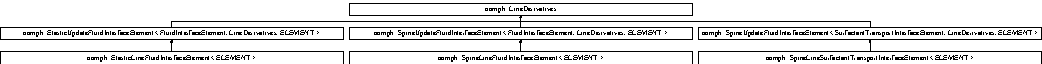
\includegraphics[height=0.861539cm]{classoomph_1_1LineDerivatives}
\end{center}
\end{figure}
\subsection*{Public Member Functions}
\begin{DoxyCompactItemize}
\item 
\hyperlink{classoomph_1_1LineDerivatives_ab8e7af32651605a82d53995caddbe7fb}{Line\+Derivatives} ()
\end{DoxyCompactItemize}
\subsection*{Protected Member Functions}
\begin{DoxyCompactItemize}
\item 
double \hyperlink{classoomph_1_1LineDerivatives_aa50209ce504b25d255f9f0a6df36c0e3}{compute\+\_\+surface\+\_\+derivatives} (const \hyperlink{classoomph_1_1Shape}{Shape} \&psi, const \hyperlink{classoomph_1_1DShape}{D\+Shape} \&dpsids, const \hyperlink{classoomph_1_1DenseMatrix}{Dense\+Matrix}$<$ double $>$ \&interpolated\+\_\+t, const \hyperlink{classoomph_1_1Vector}{Vector}$<$ double $>$ \&interpolated\+\_\+x, \hyperlink{classoomph_1_1DShape}{D\+Shape} \&surface\+\_\+gradient, \hyperlink{classoomph_1_1DShape}{D\+Shape} \&surface\+\_\+divergence)
\begin{DoxyCompactList}\small\item\em Fill in the specific surface derivative calculations. \end{DoxyCompactList}\end{DoxyCompactItemize}


\subsection{Detailed Description}
Class that establishes the surface derivative functions for Line\+Elements. These are defined in a separate class so that they can be used by other interface equation-\/type classes. 

Definition at line 644 of file interface\+\_\+elements.\+h.



\subsection{Constructor \& Destructor Documentation}
\mbox{\Hypertarget{classoomph_1_1LineDerivatives_ab8e7af32651605a82d53995caddbe7fb}\label{classoomph_1_1LineDerivatives_ab8e7af32651605a82d53995caddbe7fb}} 
\index{oomph\+::\+Line\+Derivatives@{oomph\+::\+Line\+Derivatives}!Line\+Derivatives@{Line\+Derivatives}}
\index{Line\+Derivatives@{Line\+Derivatives}!oomph\+::\+Line\+Derivatives@{oomph\+::\+Line\+Derivatives}}
\subsubsection{\texorpdfstring{Line\+Derivatives()}{LineDerivatives()}}
{\footnotesize\ttfamily oomph\+::\+Line\+Derivatives\+::\+Line\+Derivatives (\begin{DoxyParamCaption}{ }\end{DoxyParamCaption})\hspace{0.3cm}{\ttfamily [inline]}}



Definition at line 648 of file interface\+\_\+elements.\+h.



References oomph\+::\+Face\+Element\+::interpolated\+\_\+x().



\subsection{Member Function Documentation}
\mbox{\Hypertarget{classoomph_1_1LineDerivatives_aa50209ce504b25d255f9f0a6df36c0e3}\label{classoomph_1_1LineDerivatives_aa50209ce504b25d255f9f0a6df36c0e3}} 
\index{oomph\+::\+Line\+Derivatives@{oomph\+::\+Line\+Derivatives}!compute\+\_\+surface\+\_\+derivatives@{compute\+\_\+surface\+\_\+derivatives}}
\index{compute\+\_\+surface\+\_\+derivatives@{compute\+\_\+surface\+\_\+derivatives}!oomph\+::\+Line\+Derivatives@{oomph\+::\+Line\+Derivatives}}
\subsubsection{\texorpdfstring{compute\+\_\+surface\+\_\+derivatives()}{compute\_surface\_derivatives()}}
{\footnotesize\ttfamily double oomph\+::\+Line\+Derivatives\+::compute\+\_\+surface\+\_\+derivatives (\begin{DoxyParamCaption}\item[{const \hyperlink{classoomph_1_1Shape}{Shape} \&}]{psi,  }\item[{const \hyperlink{classoomph_1_1DShape}{D\+Shape} \&}]{dpsids,  }\item[{const \hyperlink{classoomph_1_1DenseMatrix}{Dense\+Matrix}$<$ double $>$ \&}]{interpolated\+\_\+t,  }\item[{const \hyperlink{classoomph_1_1Vector}{Vector}$<$ double $>$ \&}]{interpolated\+\_\+x,  }\item[{\hyperlink{classoomph_1_1DShape}{D\+Shape} \&}]{surface\+\_\+gradient,  }\item[{\hyperlink{classoomph_1_1DShape}{D\+Shape} \&}]{surface\+\_\+divergence }\end{DoxyParamCaption})\hspace{0.3cm}{\ttfamily [protected]}}



Fill in the specific surface derivative calculations. 

Specialise the surface derivatives for the line interface case. 

Definition at line 763 of file interface\+\_\+elements.\+cc.



References i, and oomph\+::\+Shape\+::nindex1().



The documentation for this class was generated from the following files\+:\begin{DoxyCompactItemize}
\item 
\hyperlink{interface__elements_8h}{interface\+\_\+elements.\+h}\item 
\hyperlink{interface__elements_8cc}{interface\+\_\+elements.\+cc}\end{DoxyCompactItemize}

\hypertarget{classoomph_1_1LineFluidInterfaceBoundingElement}{}\section{oomph\+:\+:Line\+Fluid\+Interface\+Bounding\+Element Class Reference}
\label{classoomph_1_1LineFluidInterfaceBoundingElement}\index{oomph\+::\+Line\+Fluid\+Interface\+Bounding\+Element@{oomph\+::\+Line\+Fluid\+Interface\+Bounding\+Element}}


Specialisation of the interface boundary constraint to a line.  




{\ttfamily \#include $<$interface\+\_\+elements.\+h$>$}

Inheritance diagram for oomph\+:\+:Line\+Fluid\+Interface\+Bounding\+Element\+:\begin{figure}[H]
\begin{center}
\leavevmode
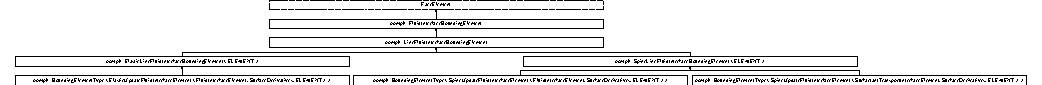
\includegraphics[height=1.593496cm]{classoomph_1_1LineFluidInterfaceBoundingElement}
\end{center}
\end{figure}
\subsection*{Public Member Functions}
\begin{DoxyCompactItemize}
\item 
\hyperlink{classoomph_1_1LineFluidInterfaceBoundingElement_a29d14ee44cd9b2db52779ea570850821}{Line\+Fluid\+Interface\+Bounding\+Element} ()
\begin{DoxyCompactList}\small\item\em Constructor. \end{DoxyCompactList}\end{DoxyCompactItemize}
\subsection*{Protected Member Functions}
\begin{DoxyCompactItemize}
\item 
void \hyperlink{classoomph_1_1LineFluidInterfaceBoundingElement_aa162a09ba8dfcba4d81e6abaa7a29986}{fill\+\_\+in\+\_\+generic\+\_\+residual\+\_\+contribution\+\_\+interface\+\_\+boundary} (\hyperlink{classoomph_1_1Vector}{Vector}$<$ double $>$ \&residuals, \hyperlink{classoomph_1_1DenseMatrix}{Dense\+Matrix}$<$ double $>$ \&jacobian, unsigned flag)
\begin{DoxyCompactList}\small\item\em Overload the helper function to calculate the residuals and (if flag==true) the Jacobian -- this function only deals with the part of the Jacobian that can be handled generically. Specific additional contributions may be provided in \hyperlink{classoomph_1_1FluidInterfaceBoundingElement_a4510bd81b572d758694715f673080041}{add\+\_\+additional\+\_\+residual\+\_\+contributions\+\_\+interface\+\_\+boundary()} \end{DoxyCompactList}\end{DoxyCompactItemize}
\subsection*{Additional Inherited Members}


\subsection{Detailed Description}
Specialisation of the interface boundary constraint to a line. 

Definition at line 289 of file interface\+\_\+elements.\+h.



\subsection{Constructor \& Destructor Documentation}
\mbox{\Hypertarget{classoomph_1_1LineFluidInterfaceBoundingElement_a29d14ee44cd9b2db52779ea570850821}\label{classoomph_1_1LineFluidInterfaceBoundingElement_a29d14ee44cd9b2db52779ea570850821}} 
\index{oomph\+::\+Line\+Fluid\+Interface\+Bounding\+Element@{oomph\+::\+Line\+Fluid\+Interface\+Bounding\+Element}!Line\+Fluid\+Interface\+Bounding\+Element@{Line\+Fluid\+Interface\+Bounding\+Element}}
\index{Line\+Fluid\+Interface\+Bounding\+Element@{Line\+Fluid\+Interface\+Bounding\+Element}!oomph\+::\+Line\+Fluid\+Interface\+Bounding\+Element@{oomph\+::\+Line\+Fluid\+Interface\+Bounding\+Element}}
\subsubsection{\texorpdfstring{Line\+Fluid\+Interface\+Bounding\+Element()}{LineFluidInterfaceBoundingElement()}}
{\footnotesize\ttfamily oomph\+::\+Line\+Fluid\+Interface\+Bounding\+Element\+::\+Line\+Fluid\+Interface\+Bounding\+Element (\begin{DoxyParamCaption}{ }\end{DoxyParamCaption})\hspace{0.3cm}{\ttfamily [inline]}}



Constructor. 



Definition at line 307 of file interface\+\_\+elements.\+h.



\subsection{Member Function Documentation}
\mbox{\Hypertarget{classoomph_1_1LineFluidInterfaceBoundingElement_aa162a09ba8dfcba4d81e6abaa7a29986}\label{classoomph_1_1LineFluidInterfaceBoundingElement_aa162a09ba8dfcba4d81e6abaa7a29986}} 
\index{oomph\+::\+Line\+Fluid\+Interface\+Bounding\+Element@{oomph\+::\+Line\+Fluid\+Interface\+Bounding\+Element}!fill\+\_\+in\+\_\+generic\+\_\+residual\+\_\+contribution\+\_\+interface\+\_\+boundary@{fill\+\_\+in\+\_\+generic\+\_\+residual\+\_\+contribution\+\_\+interface\+\_\+boundary}}
\index{fill\+\_\+in\+\_\+generic\+\_\+residual\+\_\+contribution\+\_\+interface\+\_\+boundary@{fill\+\_\+in\+\_\+generic\+\_\+residual\+\_\+contribution\+\_\+interface\+\_\+boundary}!oomph\+::\+Line\+Fluid\+Interface\+Bounding\+Element@{oomph\+::\+Line\+Fluid\+Interface\+Bounding\+Element}}
\subsubsection{\texorpdfstring{fill\+\_\+in\+\_\+generic\+\_\+residual\+\_\+contribution\+\_\+interface\+\_\+boundary()}{fill\_in\_generic\_residual\_contribution\_interface\_boundary()}}
{\footnotesize\ttfamily void oomph\+::\+Line\+Fluid\+Interface\+Bounding\+Element\+::fill\+\_\+in\+\_\+generic\+\_\+residual\+\_\+contribution\+\_\+interface\+\_\+boundary (\begin{DoxyParamCaption}\item[{\hyperlink{classoomph_1_1Vector}{Vector}$<$ double $>$ \&}]{residuals,  }\item[{\hyperlink{classoomph_1_1DenseMatrix}{Dense\+Matrix}$<$ double $>$ \&}]{jacobian,  }\item[{unsigned}]{flag }\end{DoxyParamCaption})\hspace{0.3cm}{\ttfamily [protected]}, {\ttfamily [virtual]}}



Overload the helper function to calculate the residuals and (if flag==true) the Jacobian -- this function only deals with the part of the Jacobian that can be handled generically. Specific additional contributions may be provided in \hyperlink{classoomph_1_1FluidInterfaceBoundingElement_a4510bd81b572d758694715f673080041}{add\+\_\+additional\+\_\+residual\+\_\+contributions\+\_\+interface\+\_\+boundary()} 

Add contribution to element\textquotesingle{}s residual vector and Jacobian. 

Implements \hyperlink{classoomph_1_1FluidInterfaceBoundingElement_a69fa099e0cbfe8ae028a4edc77fedc60}{oomph\+::\+Fluid\+Interface\+Bounding\+Element}.



Definition at line 238 of file interface\+\_\+elements.\+cc.



References oomph\+::\+Fluid\+Interface\+Bounding\+Element\+::add\+\_\+additional\+\_\+residual\+\_\+contributions\+\_\+interface\+\_\+boundary(), oomph\+::\+Face\+Element\+::bulk\+\_\+element\+\_\+pt(), oomph\+::\+Fluid\+Interface\+Bounding\+Element\+::ca(), oomph\+::\+Fluid\+Interface\+Bounding\+Element\+::contact\+\_\+angle(), oomph\+::\+Fluid\+Interface\+Bounding\+Element\+::\+Contact\+\_\+angle\+\_\+flag, oomph\+::\+Fluid\+Interface\+Element\+::\+Default\+\_\+\+Physical\+\_\+\+Constant\+\_\+\+Value, oomph\+::\+Finite\+Element\+::dim(), oomph\+::\+Vector\+Helpers\+::dot(), oomph\+::\+Finite\+Element\+::dshape\+\_\+local(), oomph\+::\+Face\+Element\+::get\+\_\+local\+\_\+coordinate\+\_\+in\+\_\+bulk(), i, oomph\+::\+Finite\+Element\+::integral\+\_\+pt(), oomph\+::\+Fluid\+Interface\+Element\+::interpolated\+\_\+u(), oomph\+::\+Fluid\+Interface\+Bounding\+Element\+::kinematic\+\_\+local\+\_\+eqn(), oomph\+::\+Integral\+::knot(), oomph\+::\+Finite\+Element\+::nnode(), oomph\+::\+Finite\+Element\+::nodal\+\_\+dimension(), oomph\+::\+Finite\+Element\+::nodal\+\_\+local\+\_\+eqn(), oomph\+::\+Finite\+Element\+::nodal\+\_\+position(), oomph\+::\+Integral\+::nweight(), oomph\+::\+Face\+Element\+::outer\+\_\+unit\+\_\+normal(), oomph\+::\+Fluid\+Interface\+Bounding\+Element\+::\+U\+\_\+index\+\_\+interface\+\_\+boundary, oomph\+::\+Quad\+Tree\+Names\+::W, oomph\+::\+Fluid\+Interface\+Bounding\+Element\+::wall\+\_\+unit\+\_\+normal(), and oomph\+::\+Integral\+::weight().



Referenced by oomph\+::\+Point\+Fluid\+Interface\+Bounding\+Element\+::fill\+\_\+in\+\_\+generic\+\_\+residual\+\_\+contribution\+\_\+interface\+\_\+boundary().



The documentation for this class was generated from the following files\+:\begin{DoxyCompactItemize}
\item 
\hyperlink{interface__elements_8h}{interface\+\_\+elements.\+h}\item 
\hyperlink{interface__elements_8cc}{interface\+\_\+elements.\+cc}\end{DoxyCompactItemize}

\hypertarget{classoomph_1_1LineVolumeConstraintBoundingElement}{}\section{oomph\+:\+:Line\+Volume\+Constraint\+Bounding\+Element Class Reference}
\label{classoomph_1_1LineVolumeConstraintBoundingElement}\index{oomph\+::\+Line\+Volume\+Constraint\+Bounding\+Element@{oomph\+::\+Line\+Volume\+Constraint\+Bounding\+Element}}


{\ttfamily \#include $<$constrained\+\_\+volume\+\_\+elements.\+h$>$}

Inheritance diagram for oomph\+:\+:Line\+Volume\+Constraint\+Bounding\+Element\+:\begin{figure}[H]
\begin{center}
\leavevmode
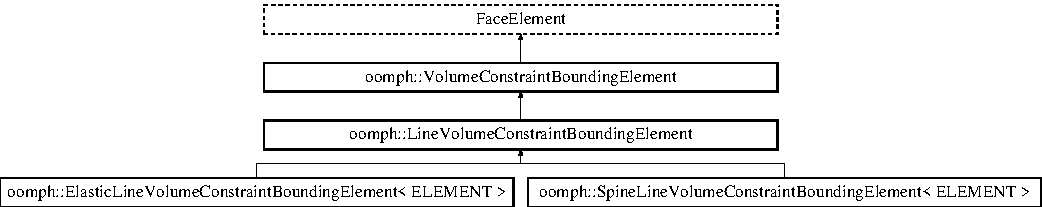
\includegraphics[height=2.786070cm]{classoomph_1_1LineVolumeConstraintBoundingElement}
\end{center}
\end{figure}
\subsection*{Public Member Functions}
\begin{DoxyCompactItemize}
\item 
\hyperlink{classoomph_1_1LineVolumeConstraintBoundingElement_a39baabe26bcf3958b80fe3dd5430c347}{Line\+Volume\+Constraint\+Bounding\+Element} ()
\begin{DoxyCompactList}\small\item\em Empty Contructor. \end{DoxyCompactList}\item 
\hyperlink{classoomph_1_1LineVolumeConstraintBoundingElement_a905d0b20f7f9a009d07c7d4506b404ed}{$\sim$\+Line\+Volume\+Constraint\+Bounding\+Element} ()
\begin{DoxyCompactList}\small\item\em Empty Destructor. \end{DoxyCompactList}\item 
double \hyperlink{classoomph_1_1LineVolumeConstraintBoundingElement_a099357dfeca3c4e1d84b0979cd495da9}{contribution\+\_\+to\+\_\+enclosed\+\_\+volume} ()
\begin{DoxyCompactList}\small\item\em Return this element\textquotesingle{}s contribution to the total volume enclosed. \end{DoxyCompactList}\end{DoxyCompactItemize}
\subsection*{Protected Member Functions}
\begin{DoxyCompactItemize}
\item 
void \hyperlink{classoomph_1_1LineVolumeConstraintBoundingElement_a03145a064e559d786f730c85000f9fb4}{fill\+\_\+in\+\_\+generic\+\_\+residual\+\_\+contribution\+\_\+volume\+\_\+constraint} (Vector$<$ double $>$ \&residuals)
\begin{DoxyCompactList}\small\item\em Helper function to fill in contributions to residuals (remember that part of the residual is added by the the associated \hyperlink{classoomph_1_1VolumeConstraintElement}{Volume\+Constraint\+Element}). This is specific for 1D line elements that bound 2D cartesian fluid elements. \end{DoxyCompactList}\end{DoxyCompactItemize}
\subsection*{Additional Inherited Members}


\subsection{Detailed Description}
One-\/dimensional interface elements that allow the application of a volume constraint on the region bounded by these elements. The volume is computed by integrating x.\+n around the boundary of the domain and then dividing by two. The sign is chosen so that the volume will be positive when the elements surround a fluid domain.

These elements must be used together with the associated \hyperlink{classoomph_1_1VolumeConstraintElement}{Volume\+Constraint\+Element}, which stores the value of the target volume. 

Definition at line 340 of file constrained\+\_\+volume\+\_\+elements.\+h.



\subsection{Constructor \& Destructor Documentation}
\mbox{\Hypertarget{classoomph_1_1LineVolumeConstraintBoundingElement_a39baabe26bcf3958b80fe3dd5430c347}\label{classoomph_1_1LineVolumeConstraintBoundingElement_a39baabe26bcf3958b80fe3dd5430c347}} 
\index{oomph\+::\+Line\+Volume\+Constraint\+Bounding\+Element@{oomph\+::\+Line\+Volume\+Constraint\+Bounding\+Element}!Line\+Volume\+Constraint\+Bounding\+Element@{Line\+Volume\+Constraint\+Bounding\+Element}}
\index{Line\+Volume\+Constraint\+Bounding\+Element@{Line\+Volume\+Constraint\+Bounding\+Element}!oomph\+::\+Line\+Volume\+Constraint\+Bounding\+Element@{oomph\+::\+Line\+Volume\+Constraint\+Bounding\+Element}}
\subsubsection{\texorpdfstring{Line\+Volume\+Constraint\+Bounding\+Element()}{LineVolumeConstraintBoundingElement()}}
{\footnotesize\ttfamily oomph\+::\+Line\+Volume\+Constraint\+Bounding\+Element\+::\+Line\+Volume\+Constraint\+Bounding\+Element (\begin{DoxyParamCaption}{ }\end{DoxyParamCaption})\hspace{0.3cm}{\ttfamily [inline]}}



Empty Contructor. 



Definition at line 355 of file constrained\+\_\+volume\+\_\+elements.\+h.

\mbox{\Hypertarget{classoomph_1_1LineVolumeConstraintBoundingElement_a905d0b20f7f9a009d07c7d4506b404ed}\label{classoomph_1_1LineVolumeConstraintBoundingElement_a905d0b20f7f9a009d07c7d4506b404ed}} 
\index{oomph\+::\+Line\+Volume\+Constraint\+Bounding\+Element@{oomph\+::\+Line\+Volume\+Constraint\+Bounding\+Element}!````~Line\+Volume\+Constraint\+Bounding\+Element@{$\sim$\+Line\+Volume\+Constraint\+Bounding\+Element}}
\index{````~Line\+Volume\+Constraint\+Bounding\+Element@{$\sim$\+Line\+Volume\+Constraint\+Bounding\+Element}!oomph\+::\+Line\+Volume\+Constraint\+Bounding\+Element@{oomph\+::\+Line\+Volume\+Constraint\+Bounding\+Element}}
\subsubsection{\texorpdfstring{$\sim$\+Line\+Volume\+Constraint\+Bounding\+Element()}{~LineVolumeConstraintBoundingElement()}}
{\footnotesize\ttfamily oomph\+::\+Line\+Volume\+Constraint\+Bounding\+Element\+::$\sim$\+Line\+Volume\+Constraint\+Bounding\+Element (\begin{DoxyParamCaption}{ }\end{DoxyParamCaption})\hspace{0.3cm}{\ttfamily [inline]}}



Empty Destructor. 



Definition at line 358 of file constrained\+\_\+volume\+\_\+elements.\+h.



\subsection{Member Function Documentation}
\mbox{\Hypertarget{classoomph_1_1LineVolumeConstraintBoundingElement_a099357dfeca3c4e1d84b0979cd495da9}\label{classoomph_1_1LineVolumeConstraintBoundingElement_a099357dfeca3c4e1d84b0979cd495da9}} 
\index{oomph\+::\+Line\+Volume\+Constraint\+Bounding\+Element@{oomph\+::\+Line\+Volume\+Constraint\+Bounding\+Element}!contribution\+\_\+to\+\_\+enclosed\+\_\+volume@{contribution\+\_\+to\+\_\+enclosed\+\_\+volume}}
\index{contribution\+\_\+to\+\_\+enclosed\+\_\+volume@{contribution\+\_\+to\+\_\+enclosed\+\_\+volume}!oomph\+::\+Line\+Volume\+Constraint\+Bounding\+Element@{oomph\+::\+Line\+Volume\+Constraint\+Bounding\+Element}}
\subsubsection{\texorpdfstring{contribution\+\_\+to\+\_\+enclosed\+\_\+volume()}{contribution\_to\_enclosed\_volume()}}
{\footnotesize\ttfamily double oomph\+::\+Line\+Volume\+Constraint\+Bounding\+Element\+::contribution\+\_\+to\+\_\+enclosed\+\_\+volume (\begin{DoxyParamCaption}{ }\end{DoxyParamCaption})}



Return this element\textquotesingle{}s contribution to the total volume enclosed. 



Definition at line 195 of file constrained\+\_\+volume\+\_\+elements.\+cc.



References oomph\+::\+Axisymmetric\+Volume\+Constraint\+Bounding\+Element\+::contribution\+\_\+to\+\_\+enclosed\+\_\+volume().

\mbox{\Hypertarget{classoomph_1_1LineVolumeConstraintBoundingElement_a03145a064e559d786f730c85000f9fb4}\label{classoomph_1_1LineVolumeConstraintBoundingElement_a03145a064e559d786f730c85000f9fb4}} 
\index{oomph\+::\+Line\+Volume\+Constraint\+Bounding\+Element@{oomph\+::\+Line\+Volume\+Constraint\+Bounding\+Element}!fill\+\_\+in\+\_\+generic\+\_\+residual\+\_\+contribution\+\_\+volume\+\_\+constraint@{fill\+\_\+in\+\_\+generic\+\_\+residual\+\_\+contribution\+\_\+volume\+\_\+constraint}}
\index{fill\+\_\+in\+\_\+generic\+\_\+residual\+\_\+contribution\+\_\+volume\+\_\+constraint@{fill\+\_\+in\+\_\+generic\+\_\+residual\+\_\+contribution\+\_\+volume\+\_\+constraint}!oomph\+::\+Line\+Volume\+Constraint\+Bounding\+Element@{oomph\+::\+Line\+Volume\+Constraint\+Bounding\+Element}}
\subsubsection{\texorpdfstring{fill\+\_\+in\+\_\+generic\+\_\+residual\+\_\+contribution\+\_\+volume\+\_\+constraint()}{fill\_in\_generic\_residual\_contribution\_volume\_constraint()}}
{\footnotesize\ttfamily void oomph\+::\+Line\+Volume\+Constraint\+Bounding\+Element\+::fill\+\_\+in\+\_\+generic\+\_\+residual\+\_\+contribution\+\_\+volume\+\_\+constraint (\begin{DoxyParamCaption}\item[{Vector$<$ double $>$ \&}]{residuals }\end{DoxyParamCaption})\hspace{0.3cm}{\ttfamily [protected]}, {\ttfamily [virtual]}}



Helper function to fill in contributions to residuals (remember that part of the residual is added by the the associated \hyperlink{classoomph_1_1VolumeConstraintElement}{Volume\+Constraint\+Element}). This is specific for 1D line elements that bound 2D cartesian fluid elements. 



Implements \hyperlink{classoomph_1_1VolumeConstraintBoundingElement_a717f1085709bd8820b8043ff94ecb0c5}{oomph\+::\+Volume\+Constraint\+Bounding\+Element}.



Definition at line 120 of file constrained\+\_\+volume\+\_\+elements.\+cc.



References oomph\+::\+Volume\+Constraint\+Element\+::ptraded\+\_\+local\+\_\+eqn().



Referenced by oomph\+::\+Volume\+Constraint\+Element\+::\+Volume\+Constraint\+Element().



The documentation for this class was generated from the following files\+:\begin{DoxyCompactItemize}
\item 
\hyperlink{constrained__volume__elements_8h}{constrained\+\_\+volume\+\_\+elements.\+h}\item 
\hyperlink{constrained__volume__elements_8cc}{constrained\+\_\+volume\+\_\+elements.\+cc}\end{DoxyCompactItemize}

\hypertarget{classoomph_1_1PointFluidInterfaceBoundingElement}{}\section{oomph\+:\+:Point\+Fluid\+Interface\+Bounding\+Element Class Reference}
\label{classoomph_1_1PointFluidInterfaceBoundingElement}\index{oomph\+::\+Point\+Fluid\+Interface\+Bounding\+Element@{oomph\+::\+Point\+Fluid\+Interface\+Bounding\+Element}}


Specialisation of the interface boundary constraint to a point.  




{\ttfamily \#include $<$interface\+\_\+elements.\+h$>$}

Inheritance diagram for oomph\+:\+:Point\+Fluid\+Interface\+Bounding\+Element\+:\begin{figure}[H]
\begin{center}
\leavevmode
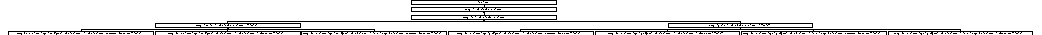
\includegraphics[height=0.468384cm]{classoomph_1_1PointFluidInterfaceBoundingElement}
\end{center}
\end{figure}
\subsection*{Public Member Functions}
\begin{DoxyCompactItemize}
\item 
\hyperlink{classoomph_1_1PointFluidInterfaceBoundingElement_a920776d9680859c72f79d446a7c3d1e8}{Point\+Fluid\+Interface\+Bounding\+Element} ()
\begin{DoxyCompactList}\small\item\em Constructor. \end{DoxyCompactList}\end{DoxyCompactItemize}
\subsection*{Protected Member Functions}
\begin{DoxyCompactItemize}
\item 
void \hyperlink{classoomph_1_1PointFluidInterfaceBoundingElement_aad95a7d6f4e4349ee1136e623aa69c88}{fill\+\_\+in\+\_\+generic\+\_\+residual\+\_\+contribution\+\_\+interface\+\_\+boundary} (Vector$<$ double $>$ \&residuals, Dense\+Matrix$<$ double $>$ \&jacobian, unsigned flag)
\begin{DoxyCompactList}\small\item\em Overload the helper function to calculate the residuals and (if flag==1) the Jacobian -- this function only deals with the part of the Jacobian that can be handled generically. Specific additional contributions may be provided in add\+\_\+additional\+\_\+residual\+\_\+contributions\+\_\+interface\+\_\+boundary(...) \end{DoxyCompactList}\end{DoxyCompactItemize}
\subsection*{Additional Inherited Members}


\subsection{Detailed Description}
Specialisation of the interface boundary constraint to a point. 

Definition at line 262 of file interface\+\_\+elements.\+h.



\subsection{Constructor \& Destructor Documentation}
\mbox{\Hypertarget{classoomph_1_1PointFluidInterfaceBoundingElement_a920776d9680859c72f79d446a7c3d1e8}\label{classoomph_1_1PointFluidInterfaceBoundingElement_a920776d9680859c72f79d446a7c3d1e8}} 
\index{oomph\+::\+Point\+Fluid\+Interface\+Bounding\+Element@{oomph\+::\+Point\+Fluid\+Interface\+Bounding\+Element}!Point\+Fluid\+Interface\+Bounding\+Element@{Point\+Fluid\+Interface\+Bounding\+Element}}
\index{Point\+Fluid\+Interface\+Bounding\+Element@{Point\+Fluid\+Interface\+Bounding\+Element}!oomph\+::\+Point\+Fluid\+Interface\+Bounding\+Element@{oomph\+::\+Point\+Fluid\+Interface\+Bounding\+Element}}
\subsubsection{\texorpdfstring{Point\+Fluid\+Interface\+Bounding\+Element()}{PointFluidInterfaceBoundingElement()}}
{\footnotesize\ttfamily oomph\+::\+Point\+Fluid\+Interface\+Bounding\+Element\+::\+Point\+Fluid\+Interface\+Bounding\+Element (\begin{DoxyParamCaption}{ }\end{DoxyParamCaption})\hspace{0.3cm}{\ttfamily [inline]}}



Constructor. 



Definition at line 280 of file interface\+\_\+elements.\+h.



\subsection{Member Function Documentation}
\mbox{\Hypertarget{classoomph_1_1PointFluidInterfaceBoundingElement_aad95a7d6f4e4349ee1136e623aa69c88}\label{classoomph_1_1PointFluidInterfaceBoundingElement_aad95a7d6f4e4349ee1136e623aa69c88}} 
\index{oomph\+::\+Point\+Fluid\+Interface\+Bounding\+Element@{oomph\+::\+Point\+Fluid\+Interface\+Bounding\+Element}!fill\+\_\+in\+\_\+generic\+\_\+residual\+\_\+contribution\+\_\+interface\+\_\+boundary@{fill\+\_\+in\+\_\+generic\+\_\+residual\+\_\+contribution\+\_\+interface\+\_\+boundary}}
\index{fill\+\_\+in\+\_\+generic\+\_\+residual\+\_\+contribution\+\_\+interface\+\_\+boundary@{fill\+\_\+in\+\_\+generic\+\_\+residual\+\_\+contribution\+\_\+interface\+\_\+boundary}!oomph\+::\+Point\+Fluid\+Interface\+Bounding\+Element@{oomph\+::\+Point\+Fluid\+Interface\+Bounding\+Element}}
\subsubsection{\texorpdfstring{fill\+\_\+in\+\_\+generic\+\_\+residual\+\_\+contribution\+\_\+interface\+\_\+boundary()}{fill\_in\_generic\_residual\_contribution\_interface\_boundary()}}
{\footnotesize\ttfamily void oomph\+::\+Point\+Fluid\+Interface\+Bounding\+Element\+::fill\+\_\+in\+\_\+generic\+\_\+residual\+\_\+contribution\+\_\+interface\+\_\+boundary (\begin{DoxyParamCaption}\item[{Vector$<$ double $>$ \&}]{residuals,  }\item[{Dense\+Matrix$<$ double $>$ \&}]{jacobian,  }\item[{unsigned}]{flag }\end{DoxyParamCaption})\hspace{0.3cm}{\ttfamily [protected]}, {\ttfamily [virtual]}}



Overload the helper function to calculate the residuals and (if flag==1) the Jacobian -- this function only deals with the part of the Jacobian that can be handled generically. Specific additional contributions may be provided in add\+\_\+additional\+\_\+residual\+\_\+contributions\+\_\+interface\+\_\+boundary(...) 

Add contribution to element\textquotesingle{}s residual vector and Jacobian. 

Implements \hyperlink{classoomph_1_1FluidInterfaceBoundingElement_a69fa099e0cbfe8ae028a4edc77fedc60}{oomph\+::\+Fluid\+Interface\+Bounding\+Element}.



Definition at line 92 of file interface\+\_\+elements.\+cc.



References oomph\+::\+Fluid\+Interface\+Bounding\+Element\+::add\+\_\+additional\+\_\+residual\+\_\+contributions\+\_\+interface\+\_\+boundary(), oomph\+::\+Fluid\+Interface\+Bounding\+Element\+::ca(), oomph\+::\+Fluid\+Interface\+Bounding\+Element\+::contact\+\_\+angle(), oomph\+::\+Fluid\+Interface\+Bounding\+Element\+::\+Contact\+\_\+angle\+\_\+flag, oomph\+::\+Line\+Fluid\+Interface\+Bounding\+Element\+::fill\+\_\+in\+\_\+generic\+\_\+residual\+\_\+contribution\+\_\+interface\+\_\+boundary(), oomph\+::\+Fluid\+Interface\+Bounding\+Element\+::kinematic\+\_\+local\+\_\+eqn(), oomph\+::\+Fluid\+Interface\+Bounding\+Element\+::\+U\+\_\+index\+\_\+interface\+\_\+boundary, and oomph\+::\+Fluid\+Interface\+Bounding\+Element\+::wall\+\_\+unit\+\_\+normal().



Referenced by oomph\+::\+Fluid\+Interface\+Bounding\+Element\+::set\+\_\+contact\+\_\+angle().



The documentation for this class was generated from the following files\+:\begin{DoxyCompactItemize}
\item 
\hyperlink{interface__elements_8h}{interface\+\_\+elements.\+h}\item 
\hyperlink{interface__elements_8cc}{interface\+\_\+elements.\+cc}\end{DoxyCompactItemize}

\hypertarget{classoomph_1_1SpineAxisymmetricFluidInterfaceElement}{}\section{oomph\+:\+:Spine\+Axisymmetric\+Fluid\+Interface\+Element$<$ E\+L\+E\+M\+E\+NT $>$ Class Template Reference}
\label{classoomph_1_1SpineAxisymmetricFluidInterfaceElement}\index{oomph\+::\+Spine\+Axisymmetric\+Fluid\+Interface\+Element$<$ E\+L\+E\+M\+E\+N\+T $>$@{oomph\+::\+Spine\+Axisymmetric\+Fluid\+Interface\+Element$<$ E\+L\+E\+M\+E\+N\+T $>$}}


{\ttfamily \#include $<$specific\+\_\+node\+\_\+update\+\_\+interface\+\_\+elements.\+h$>$}

Inheritance diagram for oomph\+:\+:Spine\+Axisymmetric\+Fluid\+Interface\+Element$<$ E\+L\+E\+M\+E\+NT $>$\+:\begin{figure}[H]
\begin{center}
\leavevmode
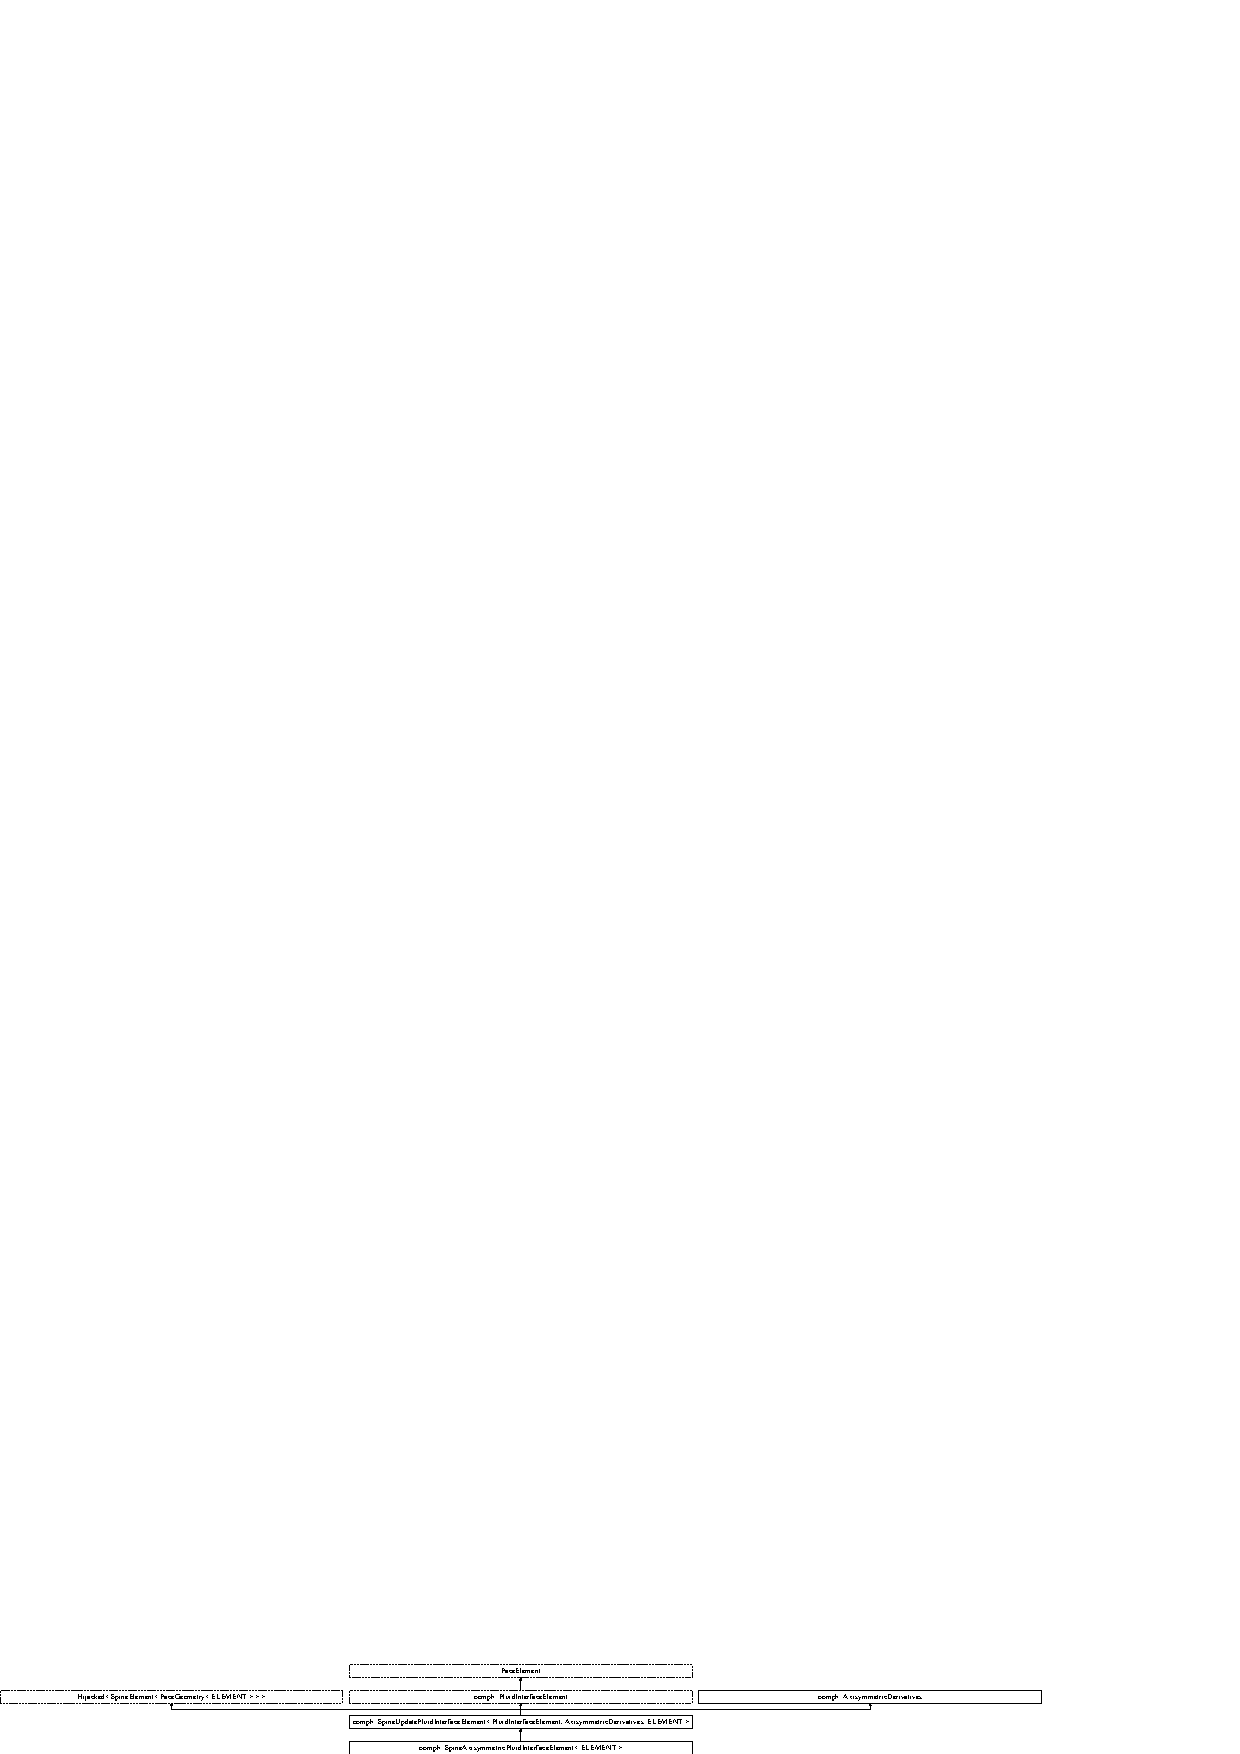
\includegraphics[height=1.454545cm]{classoomph_1_1SpineAxisymmetricFluidInterfaceElement}
\end{center}
\end{figure}
\subsection*{Public Member Functions}
\begin{DoxyCompactItemize}
\item 
\hyperlink{classoomph_1_1SpineAxisymmetricFluidInterfaceElement_a66aaa2581711338cf66660d97663d7cb}{Spine\+Axisymmetric\+Fluid\+Interface\+Element} (\hyperlink{classoomph_1_1FiniteElement}{Finite\+Element} $\ast$const \&element\+\_\+pt, const int \&\hyperlink{classoomph_1_1FaceElement_a478d577ac6db67ecc80f1f02ae3ab170}{face\+\_\+index})
\end{DoxyCompactItemize}
\subsection*{Additional Inherited Members}


\subsection{Detailed Description}
\subsubsection*{template$<$class E\+L\+E\+M\+E\+NT$>$\newline
class oomph\+::\+Spine\+Axisymmetric\+Fluid\+Interface\+Element$<$ E\+L\+E\+M\+E\+N\+T $>$}



Definition at line 525 of file specific\+\_\+node\+\_\+update\+\_\+interface\+\_\+elements.\+h.



\subsection{Constructor \& Destructor Documentation}
\mbox{\Hypertarget{classoomph_1_1SpineAxisymmetricFluidInterfaceElement_a66aaa2581711338cf66660d97663d7cb}\label{classoomph_1_1SpineAxisymmetricFluidInterfaceElement_a66aaa2581711338cf66660d97663d7cb}} 
\index{oomph\+::\+Spine\+Axisymmetric\+Fluid\+Interface\+Element@{oomph\+::\+Spine\+Axisymmetric\+Fluid\+Interface\+Element}!Spine\+Axisymmetric\+Fluid\+Interface\+Element@{Spine\+Axisymmetric\+Fluid\+Interface\+Element}}
\index{Spine\+Axisymmetric\+Fluid\+Interface\+Element@{Spine\+Axisymmetric\+Fluid\+Interface\+Element}!oomph\+::\+Spine\+Axisymmetric\+Fluid\+Interface\+Element@{oomph\+::\+Spine\+Axisymmetric\+Fluid\+Interface\+Element}}
\subsubsection{\texorpdfstring{Spine\+Axisymmetric\+Fluid\+Interface\+Element()}{SpineAxisymmetricFluidInterfaceElement()}}
{\footnotesize\ttfamily template$<$class E\+L\+E\+M\+E\+NT $>$ \\
\hyperlink{classoomph_1_1SpineAxisymmetricFluidInterfaceElement}{oomph\+::\+Spine\+Axisymmetric\+Fluid\+Interface\+Element}$<$ E\+L\+E\+M\+E\+NT $>$\+::\hyperlink{classoomph_1_1SpineAxisymmetricFluidInterfaceElement}{Spine\+Axisymmetric\+Fluid\+Interface\+Element} (\begin{DoxyParamCaption}\item[{\hyperlink{classoomph_1_1FiniteElement}{Finite\+Element} $\ast$const \&}]{element\+\_\+pt,  }\item[{const int \&}]{face\+\_\+index }\end{DoxyParamCaption})\hspace{0.3cm}{\ttfamily [inline]}}



Definition at line 531 of file specific\+\_\+node\+\_\+update\+\_\+interface\+\_\+elements.\+h.



The documentation for this class was generated from the following file\+:\begin{DoxyCompactItemize}
\item 
\hyperlink{specific__node__update__interface__elements_8h}{specific\+\_\+node\+\_\+update\+\_\+interface\+\_\+elements.\+h}\end{DoxyCompactItemize}

\hypertarget{classoomph_1_1SpineAxisymmetricSurfactantTransportInterfaceElement}{}\section{oomph\+:\+:Spine\+Axisymmetric\+Surfactant\+Transport\+Interface\+Element$<$ E\+L\+E\+M\+E\+NT $>$ Class Template Reference}
\label{classoomph_1_1SpineAxisymmetricSurfactantTransportInterfaceElement}\index{oomph\+::\+Spine\+Axisymmetric\+Surfactant\+Transport\+Interface\+Element$<$ E\+L\+E\+M\+E\+N\+T $>$@{oomph\+::\+Spine\+Axisymmetric\+Surfactant\+Transport\+Interface\+Element$<$ E\+L\+E\+M\+E\+N\+T $>$}}


Specialise to the Axisymmetric geometry.  




{\ttfamily \#include $<$surfactant\+\_\+transport\+\_\+elements.\+h$>$}

Inheritance diagram for oomph\+:\+:Spine\+Axisymmetric\+Surfactant\+Transport\+Interface\+Element$<$ E\+L\+E\+M\+E\+NT $>$\+:\begin{figure}[H]
\begin{center}
\leavevmode
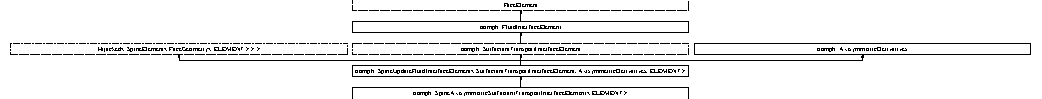
\includegraphics[height=1.280000cm]{classoomph_1_1SpineAxisymmetricSurfactantTransportInterfaceElement}
\end{center}
\end{figure}
\subsection*{Public Member Functions}
\begin{DoxyCompactItemize}
\item 
\hyperlink{classoomph_1_1SpineAxisymmetricSurfactantTransportInterfaceElement_a60ac6b568dc388e584d423d4b4e9438a}{Spine\+Axisymmetric\+Surfactant\+Transport\+Interface\+Element} (\hyperlink{classoomph_1_1FiniteElement}{Finite\+Element} $\ast$const \&element\+\_\+pt, const int \&\hyperlink{classoomph_1_1FaceElement_a478d577ac6db67ecc80f1f02ae3ab170}{face\+\_\+index})
\end{DoxyCompactItemize}
\subsection*{Additional Inherited Members}


\subsection{Detailed Description}
\subsubsection*{template$<$class E\+L\+E\+M\+E\+NT$>$\newline
class oomph\+::\+Spine\+Axisymmetric\+Surfactant\+Transport\+Interface\+Element$<$ E\+L\+E\+M\+E\+N\+T $>$}

Specialise to the Axisymmetric geometry. 

Definition at line 232 of file surfactant\+\_\+transport\+\_\+elements.\+h.



\subsection{Constructor \& Destructor Documentation}
\mbox{\Hypertarget{classoomph_1_1SpineAxisymmetricSurfactantTransportInterfaceElement_a60ac6b568dc388e584d423d4b4e9438a}\label{classoomph_1_1SpineAxisymmetricSurfactantTransportInterfaceElement_a60ac6b568dc388e584d423d4b4e9438a}} 
\index{oomph\+::\+Spine\+Axisymmetric\+Surfactant\+Transport\+Interface\+Element@{oomph\+::\+Spine\+Axisymmetric\+Surfactant\+Transport\+Interface\+Element}!Spine\+Axisymmetric\+Surfactant\+Transport\+Interface\+Element@{Spine\+Axisymmetric\+Surfactant\+Transport\+Interface\+Element}}
\index{Spine\+Axisymmetric\+Surfactant\+Transport\+Interface\+Element@{Spine\+Axisymmetric\+Surfactant\+Transport\+Interface\+Element}!oomph\+::\+Spine\+Axisymmetric\+Surfactant\+Transport\+Interface\+Element@{oomph\+::\+Spine\+Axisymmetric\+Surfactant\+Transport\+Interface\+Element}}
\subsubsection{\texorpdfstring{Spine\+Axisymmetric\+Surfactant\+Transport\+Interface\+Element()}{SpineAxisymmetricSurfactantTransportInterfaceElement()}}
{\footnotesize\ttfamily template$<$class E\+L\+E\+M\+E\+NT $>$ \\
\hyperlink{classoomph_1_1SpineAxisymmetricSurfactantTransportInterfaceElement}{oomph\+::\+Spine\+Axisymmetric\+Surfactant\+Transport\+Interface\+Element}$<$ E\+L\+E\+M\+E\+NT $>$\+::\hyperlink{classoomph_1_1SpineAxisymmetricSurfactantTransportInterfaceElement}{Spine\+Axisymmetric\+Surfactant\+Transport\+Interface\+Element} (\begin{DoxyParamCaption}\item[{\hyperlink{classoomph_1_1FiniteElement}{Finite\+Element} $\ast$const \&}]{element\+\_\+pt,  }\item[{const int \&}]{face\+\_\+index }\end{DoxyParamCaption})\hspace{0.3cm}{\ttfamily [inline]}}



Definition at line 238 of file surfactant\+\_\+transport\+\_\+elements.\+h.



The documentation for this class was generated from the following file\+:\begin{DoxyCompactItemize}
\item 
\hyperlink{surfactant__transport__elements_8h}{surfactant\+\_\+transport\+\_\+elements.\+h}\end{DoxyCompactItemize}

\hypertarget{classoomph_1_1SpineAxisymmetricVolumeConstraintBoundingElement}{}\section{oomph\+:\+:Spine\+Axisymmetric\+Volume\+Constraint\+Bounding\+Element$<$ E\+L\+E\+M\+E\+NT $>$ Class Template Reference}
\label{classoomph_1_1SpineAxisymmetricVolumeConstraintBoundingElement}\index{oomph\+::\+Spine\+Axisymmetric\+Volume\+Constraint\+Bounding\+Element$<$ E\+L\+E\+M\+E\+N\+T $>$@{oomph\+::\+Spine\+Axisymmetric\+Volume\+Constraint\+Bounding\+Element$<$ E\+L\+E\+M\+E\+N\+T $>$}}


{\ttfamily \#include $<$constrained\+\_\+volume\+\_\+elements.\+h$>$}

Inheritance diagram for oomph\+:\+:Spine\+Axisymmetric\+Volume\+Constraint\+Bounding\+Element$<$ E\+L\+E\+M\+E\+NT $>$\+:\begin{figure}[H]
\begin{center}
\leavevmode
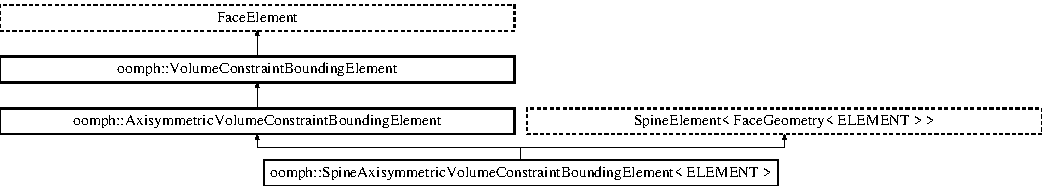
\includegraphics[height=1.631068cm]{classoomph_1_1SpineAxisymmetricVolumeConstraintBoundingElement}
\end{center}
\end{figure}
\subsection*{Public Member Functions}
\begin{DoxyCompactItemize}
\item 
\hyperlink{classoomph_1_1SpineAxisymmetricVolumeConstraintBoundingElement_a5b9c09e04e27442d00950c9bf513657e}{Spine\+Axisymmetric\+Volume\+Constraint\+Bounding\+Element} (\hyperlink{classoomph_1_1FiniteElement}{Finite\+Element} $\ast$const \&element\+\_\+pt, const int \&\hyperlink{classoomph_1_1FaceElement_a478d577ac6db67ecc80f1f02ae3ab170}{face\+\_\+index})
\begin{DoxyCompactList}\small\item\em Contructor\+: Specify bulk element and index of face to which this face element is to be attached. \end{DoxyCompactList}\item 
void \hyperlink{classoomph_1_1SpineAxisymmetricVolumeConstraintBoundingElement_a5813860802c0474ef6ff5f249ca7141f}{fill\+\_\+in\+\_\+contribution\+\_\+to\+\_\+jacobian} (\hyperlink{classoomph_1_1Vector}{Vector}$<$ double $>$ \&residuals, \hyperlink{classoomph_1_1DenseMatrix}{Dense\+Matrix}$<$ double $>$ \&jacobian)
\item 
double \hyperlink{classoomph_1_1SpineAxisymmetricVolumeConstraintBoundingElement_ae15b2d0563f79ea10d23a1286831143a}{zeta\+\_\+nodal} (const unsigned \&n, const unsigned \&k, const unsigned \&\hyperlink{cfortran_8h_adb50e893b86b3e55e751a42eab3cba82}{i}) const
\begin{DoxyCompactList}\small\item\em The \char`\"{}global\char`\"{} intrinsic coordinate of the element when viewed as part of a geometric object should be given by the \hyperlink{classoomph_1_1FaceElement}{Face\+Element} representation, by default. \end{DoxyCompactList}\end{DoxyCompactItemize}
\subsection*{Additional Inherited Members}


\subsection{Detailed Description}
\subsubsection*{template$<$class E\+L\+E\+M\+E\+NT$>$\newline
class oomph\+::\+Spine\+Axisymmetric\+Volume\+Constraint\+Bounding\+Element$<$ E\+L\+E\+M\+E\+N\+T $>$}

The axisymmetric (one-\/dimensional) interface elements that allow imposition of a volume constraint specialised for the case when the nodal positions of the bulk elements are adjusted using Spines. To enforce that a fluid volume has a certain volume, attach these elements to all faces of the (2D axisymmetric) bulk fluid elements (of type E\+L\+E\+M\+E\+NT) that bound that region and then specify the \char`\"{}pressure\char`\"{} value that is traded for the constraint. 

Definition at line 667 of file constrained\+\_\+volume\+\_\+elements.\+h.



\subsection{Constructor \& Destructor Documentation}
\mbox{\Hypertarget{classoomph_1_1SpineAxisymmetricVolumeConstraintBoundingElement_a5b9c09e04e27442d00950c9bf513657e}\label{classoomph_1_1SpineAxisymmetricVolumeConstraintBoundingElement_a5b9c09e04e27442d00950c9bf513657e}} 
\index{oomph\+::\+Spine\+Axisymmetric\+Volume\+Constraint\+Bounding\+Element@{oomph\+::\+Spine\+Axisymmetric\+Volume\+Constraint\+Bounding\+Element}!Spine\+Axisymmetric\+Volume\+Constraint\+Bounding\+Element@{Spine\+Axisymmetric\+Volume\+Constraint\+Bounding\+Element}}
\index{Spine\+Axisymmetric\+Volume\+Constraint\+Bounding\+Element@{Spine\+Axisymmetric\+Volume\+Constraint\+Bounding\+Element}!oomph\+::\+Spine\+Axisymmetric\+Volume\+Constraint\+Bounding\+Element@{oomph\+::\+Spine\+Axisymmetric\+Volume\+Constraint\+Bounding\+Element}}
\subsubsection{\texorpdfstring{Spine\+Axisymmetric\+Volume\+Constraint\+Bounding\+Element()}{SpineAxisymmetricVolumeConstraintBoundingElement()}}
{\footnotesize\ttfamily template$<$class E\+L\+E\+M\+E\+NT $>$ \\
\hyperlink{classoomph_1_1SpineAxisymmetricVolumeConstraintBoundingElement}{oomph\+::\+Spine\+Axisymmetric\+Volume\+Constraint\+Bounding\+Element}$<$ E\+L\+E\+M\+E\+NT $>$\+::\hyperlink{classoomph_1_1SpineAxisymmetricVolumeConstraintBoundingElement}{Spine\+Axisymmetric\+Volume\+Constraint\+Bounding\+Element} (\begin{DoxyParamCaption}\item[{\hyperlink{classoomph_1_1FiniteElement}{Finite\+Element} $\ast$const \&}]{element\+\_\+pt,  }\item[{const int \&}]{face\+\_\+index }\end{DoxyParamCaption})\hspace{0.3cm}{\ttfamily [inline]}}



Contructor\+: Specify bulk element and index of face to which this face element is to be attached. 



Definition at line 676 of file constrained\+\_\+volume\+\_\+elements.\+h.



References oomph\+::\+Finite\+Element\+::build\+\_\+face\+\_\+element().



\subsection{Member Function Documentation}
\mbox{\Hypertarget{classoomph_1_1SpineAxisymmetricVolumeConstraintBoundingElement_a5813860802c0474ef6ff5f249ca7141f}\label{classoomph_1_1SpineAxisymmetricVolumeConstraintBoundingElement_a5813860802c0474ef6ff5f249ca7141f}} 
\index{oomph\+::\+Spine\+Axisymmetric\+Volume\+Constraint\+Bounding\+Element@{oomph\+::\+Spine\+Axisymmetric\+Volume\+Constraint\+Bounding\+Element}!fill\+\_\+in\+\_\+contribution\+\_\+to\+\_\+jacobian@{fill\+\_\+in\+\_\+contribution\+\_\+to\+\_\+jacobian}}
\index{fill\+\_\+in\+\_\+contribution\+\_\+to\+\_\+jacobian@{fill\+\_\+in\+\_\+contribution\+\_\+to\+\_\+jacobian}!oomph\+::\+Spine\+Axisymmetric\+Volume\+Constraint\+Bounding\+Element@{oomph\+::\+Spine\+Axisymmetric\+Volume\+Constraint\+Bounding\+Element}}
\subsubsection{\texorpdfstring{fill\+\_\+in\+\_\+contribution\+\_\+to\+\_\+jacobian()}{fill\_in\_contribution\_to\_jacobian()}}
{\footnotesize\ttfamily template$<$class E\+L\+E\+M\+E\+NT $>$ \\
void \hyperlink{classoomph_1_1SpineAxisymmetricVolumeConstraintBoundingElement}{oomph\+::\+Spine\+Axisymmetric\+Volume\+Constraint\+Bounding\+Element}$<$ E\+L\+E\+M\+E\+NT $>$\+::fill\+\_\+in\+\_\+contribution\+\_\+to\+\_\+jacobian (\begin{DoxyParamCaption}\item[{\hyperlink{classoomph_1_1Vector}{Vector}$<$ double $>$ \&}]{residuals,  }\item[{\hyperlink{classoomph_1_1DenseMatrix}{Dense\+Matrix}$<$ double $>$ \&}]{jacobian }\end{DoxyParamCaption})\hspace{0.3cm}{\ttfamily [inline]}, {\ttfamily [virtual]}}

Fill in contribution to residuals and Jacobian. This is specific to spine based elements in which the shape derivatives are evaluated using geometric data 

Reimplemented from \hyperlink{classoomph_1_1GeneralisedElement_a6ae09fc0d68e4309ac1b03583d252845}{oomph\+::\+Generalised\+Element}.



Definition at line 690 of file constrained\+\_\+volume\+\_\+elements.\+h.

\mbox{\Hypertarget{classoomph_1_1SpineAxisymmetricVolumeConstraintBoundingElement_ae15b2d0563f79ea10d23a1286831143a}\label{classoomph_1_1SpineAxisymmetricVolumeConstraintBoundingElement_ae15b2d0563f79ea10d23a1286831143a}} 
\index{oomph\+::\+Spine\+Axisymmetric\+Volume\+Constraint\+Bounding\+Element@{oomph\+::\+Spine\+Axisymmetric\+Volume\+Constraint\+Bounding\+Element}!zeta\+\_\+nodal@{zeta\+\_\+nodal}}
\index{zeta\+\_\+nodal@{zeta\+\_\+nodal}!oomph\+::\+Spine\+Axisymmetric\+Volume\+Constraint\+Bounding\+Element@{oomph\+::\+Spine\+Axisymmetric\+Volume\+Constraint\+Bounding\+Element}}
\subsubsection{\texorpdfstring{zeta\+\_\+nodal()}{zeta\_nodal()}}
{\footnotesize\ttfamily template$<$class E\+L\+E\+M\+E\+NT $>$ \\
double \hyperlink{classoomph_1_1SpineAxisymmetricVolumeConstraintBoundingElement}{oomph\+::\+Spine\+Axisymmetric\+Volume\+Constraint\+Bounding\+Element}$<$ E\+L\+E\+M\+E\+NT $>$\+::zeta\+\_\+nodal (\begin{DoxyParamCaption}\item[{const unsigned \&}]{n,  }\item[{const unsigned \&}]{k,  }\item[{const unsigned \&}]{i }\end{DoxyParamCaption}) const\hspace{0.3cm}{\ttfamily [inline]}, {\ttfamily [virtual]}}



The \char`\"{}global\char`\"{} intrinsic coordinate of the element when viewed as part of a geometric object should be given by the \hyperlink{classoomph_1_1FaceElement}{Face\+Element} representation, by default. 



Reimplemented from \hyperlink{classoomph_1_1FiniteElement_a849561c5fbcbc07dc49d2dc6cca68559}{oomph\+::\+Finite\+Element}.



Definition at line 703 of file constrained\+\_\+volume\+\_\+elements.\+h.



References oomph\+::\+Face\+Element\+::zeta\+\_\+nodal().



The documentation for this class was generated from the following file\+:\begin{DoxyCompactItemize}
\item 
\hyperlink{constrained__volume__elements_8h}{constrained\+\_\+volume\+\_\+elements.\+h}\end{DoxyCompactItemize}

\hypertarget{classoomph_1_1SpineLineFluidInterfaceBoundingElement}{}\section{oomph\+:\+:Spine\+Line\+Fluid\+Interface\+Bounding\+Element$<$ E\+L\+E\+M\+E\+NT $>$ Class Template Reference}
\label{classoomph_1_1SpineLineFluidInterfaceBoundingElement}\index{oomph\+::\+Spine\+Line\+Fluid\+Interface\+Bounding\+Element$<$ E\+L\+E\+M\+E\+N\+T $>$@{oomph\+::\+Spine\+Line\+Fluid\+Interface\+Bounding\+Element$<$ E\+L\+E\+M\+E\+N\+T $>$}}


\hyperlink{classoomph_1_1Spine}{Spine} version of the \hyperlink{classoomph_1_1LineFluidInterfaceBoundingElement}{Line\+Fluid\+Interface\+Bounding\+Element}.  




{\ttfamily \#include $<$specific\+\_\+node\+\_\+update\+\_\+interface\+\_\+elements.\+h$>$}

Inheritance diagram for oomph\+:\+:Spine\+Line\+Fluid\+Interface\+Bounding\+Element$<$ E\+L\+E\+M\+E\+NT $>$\+:\begin{figure}[H]
\begin{center}
\leavevmode
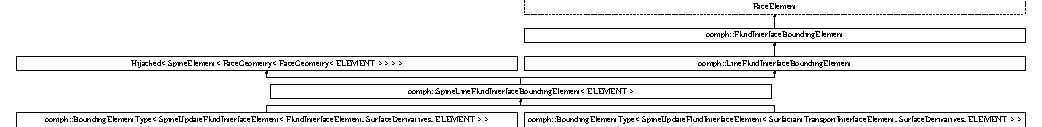
\includegraphics[height=1.092683cm]{classoomph_1_1SpineLineFluidInterfaceBoundingElement}
\end{center}
\end{figure}
\subsection*{Public Member Functions}
\begin{DoxyCompactItemize}
\item 
\hyperlink{classoomph_1_1SpineLineFluidInterfaceBoundingElement_a27c79d149485d2269ed42136914635e1}{Spine\+Line\+Fluid\+Interface\+Bounding\+Element} ()
\begin{DoxyCompactList}\small\item\em Constructor. \end{DoxyCompactList}\item 
void \hyperlink{classoomph_1_1SpineLineFluidInterfaceBoundingElement_a5c074690d693fa7fb349b22e926064b4}{output} (std\+::ostream \&outfile)
\begin{DoxyCompactList}\small\item\em Overload the output function. \end{DoxyCompactList}\item 
void \hyperlink{classoomph_1_1SpineLineFluidInterfaceBoundingElement_a77acf17ce730f50acd0d850e7460fc4d}{output} (std\+::ostream \&outfile, const unsigned \&n\+\_\+plot)
\begin{DoxyCompactList}\small\item\em Output the element. \end{DoxyCompactList}\item 
void \hyperlink{classoomph_1_1SpineLineFluidInterfaceBoundingElement_ab34fbdcd7785ab6a731a3b5d50896829}{output} (F\+I\+LE $\ast$file\+\_\+pt)
\begin{DoxyCompactList}\small\item\em Overload the C-\/style output function. \end{DoxyCompactList}\item 
void \hyperlink{classoomph_1_1SpineLineFluidInterfaceBoundingElement_ab1dbf8b8c22f78d08d431e06db80793a}{output} (F\+I\+LE $\ast$file\+\_\+pt, const unsigned \&n\+\_\+plot)
\begin{DoxyCompactList}\small\item\em C-\/style Output function. \end{DoxyCompactList}\item 
void \hyperlink{classoomph_1_1SpineLineFluidInterfaceBoundingElement_a3f44f30b5cdc47b997dbc3fd463d2038}{fill\+\_\+in\+\_\+contribution\+\_\+to\+\_\+jacobian} (\hyperlink{classoomph_1_1Vector}{Vector}$<$ double $>$ \&residuals, \hyperlink{classoomph_1_1DenseMatrix}{Dense\+Matrix}$<$ double $>$ \&jacobian)
\begin{DoxyCompactList}\small\item\em Calculate the jacobian. \end{DoxyCompactList}\item 
int \hyperlink{classoomph_1_1SpineLineFluidInterfaceBoundingElement_a0c31dba3e151540261753679b431b04a}{kinematic\+\_\+local\+\_\+eqn} (const unsigned \&n)
\begin{DoxyCompactList}\small\item\em Local eqn number of the kinematic bc associated with local node n. \end{DoxyCompactList}\end{DoxyCompactItemize}
\subsection*{Additional Inherited Members}


\subsection{Detailed Description}
\subsubsection*{template$<$class E\+L\+E\+M\+E\+NT$>$\newline
class oomph\+::\+Spine\+Line\+Fluid\+Interface\+Bounding\+Element$<$ E\+L\+E\+M\+E\+N\+T $>$}

\hyperlink{classoomph_1_1Spine}{Spine} version of the \hyperlink{classoomph_1_1LineFluidInterfaceBoundingElement}{Line\+Fluid\+Interface\+Bounding\+Element}. 

Definition at line 438 of file specific\+\_\+node\+\_\+update\+\_\+interface\+\_\+elements.\+h.



\subsection{Constructor \& Destructor Documentation}
\mbox{\Hypertarget{classoomph_1_1SpineLineFluidInterfaceBoundingElement_a27c79d149485d2269ed42136914635e1}\label{classoomph_1_1SpineLineFluidInterfaceBoundingElement_a27c79d149485d2269ed42136914635e1}} 
\index{oomph\+::\+Spine\+Line\+Fluid\+Interface\+Bounding\+Element@{oomph\+::\+Spine\+Line\+Fluid\+Interface\+Bounding\+Element}!Spine\+Line\+Fluid\+Interface\+Bounding\+Element@{Spine\+Line\+Fluid\+Interface\+Bounding\+Element}}
\index{Spine\+Line\+Fluid\+Interface\+Bounding\+Element@{Spine\+Line\+Fluid\+Interface\+Bounding\+Element}!oomph\+::\+Spine\+Line\+Fluid\+Interface\+Bounding\+Element@{oomph\+::\+Spine\+Line\+Fluid\+Interface\+Bounding\+Element}}
\subsubsection{\texorpdfstring{Spine\+Line\+Fluid\+Interface\+Bounding\+Element()}{SpineLineFluidInterfaceBoundingElement()}}
{\footnotesize\ttfamily template$<$class E\+L\+E\+M\+E\+NT $>$ \\
\hyperlink{classoomph_1_1SpineLineFluidInterfaceBoundingElement}{oomph\+::\+Spine\+Line\+Fluid\+Interface\+Bounding\+Element}$<$ E\+L\+E\+M\+E\+NT $>$\+::\hyperlink{classoomph_1_1SpineLineFluidInterfaceBoundingElement}{Spine\+Line\+Fluid\+Interface\+Bounding\+Element} (\begin{DoxyParamCaption}{ }\end{DoxyParamCaption})\hspace{0.3cm}{\ttfamily [inline]}}



Constructor. 



Definition at line 446 of file specific\+\_\+node\+\_\+update\+\_\+interface\+\_\+elements.\+h.



\subsection{Member Function Documentation}
\mbox{\Hypertarget{classoomph_1_1SpineLineFluidInterfaceBoundingElement_a3f44f30b5cdc47b997dbc3fd463d2038}\label{classoomph_1_1SpineLineFluidInterfaceBoundingElement_a3f44f30b5cdc47b997dbc3fd463d2038}} 
\index{oomph\+::\+Spine\+Line\+Fluid\+Interface\+Bounding\+Element@{oomph\+::\+Spine\+Line\+Fluid\+Interface\+Bounding\+Element}!fill\+\_\+in\+\_\+contribution\+\_\+to\+\_\+jacobian@{fill\+\_\+in\+\_\+contribution\+\_\+to\+\_\+jacobian}}
\index{fill\+\_\+in\+\_\+contribution\+\_\+to\+\_\+jacobian@{fill\+\_\+in\+\_\+contribution\+\_\+to\+\_\+jacobian}!oomph\+::\+Spine\+Line\+Fluid\+Interface\+Bounding\+Element@{oomph\+::\+Spine\+Line\+Fluid\+Interface\+Bounding\+Element}}
\subsubsection{\texorpdfstring{fill\+\_\+in\+\_\+contribution\+\_\+to\+\_\+jacobian()}{fill\_in\_contribution\_to\_jacobian()}}
{\footnotesize\ttfamily template$<$class E\+L\+E\+M\+E\+NT $>$ \\
void \hyperlink{classoomph_1_1SpineLineFluidInterfaceBoundingElement}{oomph\+::\+Spine\+Line\+Fluid\+Interface\+Bounding\+Element}$<$ E\+L\+E\+M\+E\+NT $>$\+::fill\+\_\+in\+\_\+contribution\+\_\+to\+\_\+jacobian (\begin{DoxyParamCaption}\item[{\hyperlink{classoomph_1_1Vector}{Vector}$<$ double $>$ \&}]{residuals,  }\item[{\hyperlink{classoomph_1_1DenseMatrix}{Dense\+Matrix}$<$ double $>$ \&}]{jacobian }\end{DoxyParamCaption})\hspace{0.3cm}{\ttfamily [inline]}, {\ttfamily [virtual]}}



Calculate the jacobian. 



Reimplemented from \hyperlink{classoomph_1_1GeneralisedElement_a6ae09fc0d68e4309ac1b03583d252845}{oomph\+::\+Generalised\+Element}.



Definition at line 466 of file specific\+\_\+node\+\_\+update\+\_\+interface\+\_\+elements.\+h.

\mbox{\Hypertarget{classoomph_1_1SpineLineFluidInterfaceBoundingElement_a0c31dba3e151540261753679b431b04a}\label{classoomph_1_1SpineLineFluidInterfaceBoundingElement_a0c31dba3e151540261753679b431b04a}} 
\index{oomph\+::\+Spine\+Line\+Fluid\+Interface\+Bounding\+Element@{oomph\+::\+Spine\+Line\+Fluid\+Interface\+Bounding\+Element}!kinematic\+\_\+local\+\_\+eqn@{kinematic\+\_\+local\+\_\+eqn}}
\index{kinematic\+\_\+local\+\_\+eqn@{kinematic\+\_\+local\+\_\+eqn}!oomph\+::\+Spine\+Line\+Fluid\+Interface\+Bounding\+Element@{oomph\+::\+Spine\+Line\+Fluid\+Interface\+Bounding\+Element}}
\subsubsection{\texorpdfstring{kinematic\+\_\+local\+\_\+eqn()}{kinematic\_local\_eqn()}}
{\footnotesize\ttfamily template$<$class E\+L\+E\+M\+E\+NT $>$ \\
int \hyperlink{classoomph_1_1SpineLineFluidInterfaceBoundingElement}{oomph\+::\+Spine\+Line\+Fluid\+Interface\+Bounding\+Element}$<$ E\+L\+E\+M\+E\+NT $>$\+::kinematic\+\_\+local\+\_\+eqn (\begin{DoxyParamCaption}\item[{const unsigned \&}]{n }\end{DoxyParamCaption})\hspace{0.3cm}{\ttfamily [inline]}, {\ttfamily [virtual]}}



Local eqn number of the kinematic bc associated with local node n. 



Implements \hyperlink{classoomph_1_1FluidInterfaceBoundingElement_a12a0a6d7c3c1c1a5a0f42a57e60eab34}{oomph\+::\+Fluid\+Interface\+Bounding\+Element}.



Definition at line 481 of file specific\+\_\+node\+\_\+update\+\_\+interface\+\_\+elements.\+h.

\mbox{\Hypertarget{classoomph_1_1SpineLineFluidInterfaceBoundingElement_a5c074690d693fa7fb349b22e926064b4}\label{classoomph_1_1SpineLineFluidInterfaceBoundingElement_a5c074690d693fa7fb349b22e926064b4}} 
\index{oomph\+::\+Spine\+Line\+Fluid\+Interface\+Bounding\+Element@{oomph\+::\+Spine\+Line\+Fluid\+Interface\+Bounding\+Element}!output@{output}}
\index{output@{output}!oomph\+::\+Spine\+Line\+Fluid\+Interface\+Bounding\+Element@{oomph\+::\+Spine\+Line\+Fluid\+Interface\+Bounding\+Element}}
\subsubsection{\texorpdfstring{output()}{output()}\hspace{0.1cm}{\footnotesize\ttfamily [1/4]}}
{\footnotesize\ttfamily template$<$class E\+L\+E\+M\+E\+NT $>$ \\
void \hyperlink{classoomph_1_1SpineLineFluidInterfaceBoundingElement}{oomph\+::\+Spine\+Line\+Fluid\+Interface\+Bounding\+Element}$<$ E\+L\+E\+M\+E\+NT $>$\+::output (\begin{DoxyParamCaption}\item[{std\+::ostream \&}]{outfile }\end{DoxyParamCaption})\hspace{0.3cm}{\ttfamily [inline]}, {\ttfamily [virtual]}}



Overload the output function. 



Reimplemented from \hyperlink{classoomph_1_1FluidInterfaceBoundingElement_a81adc5ae89ddfa120f587c61b972622f}{oomph\+::\+Fluid\+Interface\+Bounding\+Element}.



Definition at line 451 of file specific\+\_\+node\+\_\+update\+\_\+interface\+\_\+elements.\+h.



References oomph\+::\+Finite\+Element\+::output().

\mbox{\Hypertarget{classoomph_1_1SpineLineFluidInterfaceBoundingElement_a77acf17ce730f50acd0d850e7460fc4d}\label{classoomph_1_1SpineLineFluidInterfaceBoundingElement_a77acf17ce730f50acd0d850e7460fc4d}} 
\index{oomph\+::\+Spine\+Line\+Fluid\+Interface\+Bounding\+Element@{oomph\+::\+Spine\+Line\+Fluid\+Interface\+Bounding\+Element}!output@{output}}
\index{output@{output}!oomph\+::\+Spine\+Line\+Fluid\+Interface\+Bounding\+Element@{oomph\+::\+Spine\+Line\+Fluid\+Interface\+Bounding\+Element}}
\subsubsection{\texorpdfstring{output()}{output()}\hspace{0.1cm}{\footnotesize\ttfamily [2/4]}}
{\footnotesize\ttfamily template$<$class E\+L\+E\+M\+E\+NT $>$ \\
void \hyperlink{classoomph_1_1SpineLineFluidInterfaceBoundingElement}{oomph\+::\+Spine\+Line\+Fluid\+Interface\+Bounding\+Element}$<$ E\+L\+E\+M\+E\+NT $>$\+::output (\begin{DoxyParamCaption}\item[{std\+::ostream \&}]{outfile,  }\item[{const unsigned \&}]{n\+\_\+plot }\end{DoxyParamCaption})\hspace{0.3cm}{\ttfamily [inline]}, {\ttfamily [virtual]}}



Output the element. 



Reimplemented from \hyperlink{classoomph_1_1FluidInterfaceBoundingElement_af2c821d51d506221976a0c17e1615ac3}{oomph\+::\+Fluid\+Interface\+Bounding\+Element}.



Definition at line 454 of file specific\+\_\+node\+\_\+update\+\_\+interface\+\_\+elements.\+h.



References oomph\+::\+Fluid\+Interface\+Bounding\+Element\+::output().

\mbox{\Hypertarget{classoomph_1_1SpineLineFluidInterfaceBoundingElement_ab34fbdcd7785ab6a731a3b5d50896829}\label{classoomph_1_1SpineLineFluidInterfaceBoundingElement_ab34fbdcd7785ab6a731a3b5d50896829}} 
\index{oomph\+::\+Spine\+Line\+Fluid\+Interface\+Bounding\+Element@{oomph\+::\+Spine\+Line\+Fluid\+Interface\+Bounding\+Element}!output@{output}}
\index{output@{output}!oomph\+::\+Spine\+Line\+Fluid\+Interface\+Bounding\+Element@{oomph\+::\+Spine\+Line\+Fluid\+Interface\+Bounding\+Element}}
\subsubsection{\texorpdfstring{output()}{output()}\hspace{0.1cm}{\footnotesize\ttfamily [3/4]}}
{\footnotesize\ttfamily template$<$class E\+L\+E\+M\+E\+NT $>$ \\
void \hyperlink{classoomph_1_1SpineLineFluidInterfaceBoundingElement}{oomph\+::\+Spine\+Line\+Fluid\+Interface\+Bounding\+Element}$<$ E\+L\+E\+M\+E\+NT $>$\+::output (\begin{DoxyParamCaption}\item[{F\+I\+LE $\ast$}]{file\+\_\+pt }\end{DoxyParamCaption})\hspace{0.3cm}{\ttfamily [inline]}, {\ttfamily [virtual]}}



Overload the C-\/style output function. 



Reimplemented from \hyperlink{classoomph_1_1FluidInterfaceBoundingElement_a85cc62405429744e3e3585894315cb9e}{oomph\+::\+Fluid\+Interface\+Bounding\+Element}.



Definition at line 458 of file specific\+\_\+node\+\_\+update\+\_\+interface\+\_\+elements.\+h.



References oomph\+::\+Finite\+Element\+::output().

\mbox{\Hypertarget{classoomph_1_1SpineLineFluidInterfaceBoundingElement_ab1dbf8b8c22f78d08d431e06db80793a}\label{classoomph_1_1SpineLineFluidInterfaceBoundingElement_ab1dbf8b8c22f78d08d431e06db80793a}} 
\index{oomph\+::\+Spine\+Line\+Fluid\+Interface\+Bounding\+Element@{oomph\+::\+Spine\+Line\+Fluid\+Interface\+Bounding\+Element}!output@{output}}
\index{output@{output}!oomph\+::\+Spine\+Line\+Fluid\+Interface\+Bounding\+Element@{oomph\+::\+Spine\+Line\+Fluid\+Interface\+Bounding\+Element}}
\subsubsection{\texorpdfstring{output()}{output()}\hspace{0.1cm}{\footnotesize\ttfamily [4/4]}}
{\footnotesize\ttfamily template$<$class E\+L\+E\+M\+E\+NT $>$ \\
void \hyperlink{classoomph_1_1SpineLineFluidInterfaceBoundingElement}{oomph\+::\+Spine\+Line\+Fluid\+Interface\+Bounding\+Element}$<$ E\+L\+E\+M\+E\+NT $>$\+::output (\begin{DoxyParamCaption}\item[{F\+I\+LE $\ast$}]{file\+\_\+pt,  }\item[{const unsigned \&}]{n\+\_\+plot }\end{DoxyParamCaption})\hspace{0.3cm}{\ttfamily [inline]}, {\ttfamily [virtual]}}



C-\/style Output function. 



Reimplemented from \hyperlink{classoomph_1_1FluidInterfaceBoundingElement_ae85ea987a06275a03ad6d0e3710871da}{oomph\+::\+Fluid\+Interface\+Bounding\+Element}.



Definition at line 461 of file specific\+\_\+node\+\_\+update\+\_\+interface\+\_\+elements.\+h.



References oomph\+::\+Fluid\+Interface\+Bounding\+Element\+::output().



The documentation for this class was generated from the following file\+:\begin{DoxyCompactItemize}
\item 
\hyperlink{specific__node__update__interface__elements_8h}{specific\+\_\+node\+\_\+update\+\_\+interface\+\_\+elements.\+h}\end{DoxyCompactItemize}

\hypertarget{classoomph_1_1SpineLineFluidInterfaceElement}{}\section{oomph\+:\+:Spine\+Line\+Fluid\+Interface\+Element$<$ E\+L\+E\+M\+E\+NT $>$ Class Template Reference}
\label{classoomph_1_1SpineLineFluidInterfaceElement}\index{oomph\+::\+Spine\+Line\+Fluid\+Interface\+Element$<$ E\+L\+E\+M\+E\+N\+T $>$@{oomph\+::\+Spine\+Line\+Fluid\+Interface\+Element$<$ E\+L\+E\+M\+E\+N\+T $>$}}


{\ttfamily \#include $<$specific\+\_\+node\+\_\+update\+\_\+interface\+\_\+elements.\+h$>$}

Inheritance diagram for oomph\+:\+:Spine\+Line\+Fluid\+Interface\+Element$<$ E\+L\+E\+M\+E\+NT $>$\+:\begin{figure}[H]
\begin{center}
\leavevmode
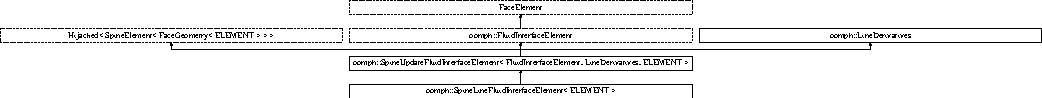
\includegraphics[height=1.583039cm]{classoomph_1_1SpineLineFluidInterfaceElement}
\end{center}
\end{figure}
\subsection*{Public Member Functions}
\begin{DoxyCompactItemize}
\item 
\hyperlink{classoomph_1_1SpineLineFluidInterfaceElement_aaafc180606b418920b0588532f8bfbec}{Spine\+Line\+Fluid\+Interface\+Element} (\hyperlink{classoomph_1_1FiniteElement}{Finite\+Element} $\ast$const \&element\+\_\+pt, const int \&\hyperlink{classoomph_1_1FaceElement_a478d577ac6db67ecc80f1f02ae3ab170}{face\+\_\+index})
\end{DoxyCompactItemize}
\subsection*{Additional Inherited Members}


\subsection{Detailed Description}
\subsubsection*{template$<$class E\+L\+E\+M\+E\+NT$>$\newline
class oomph\+::\+Spine\+Line\+Fluid\+Interface\+Element$<$ E\+L\+E\+M\+E\+N\+T $>$}



Definition at line 495 of file specific\+\_\+node\+\_\+update\+\_\+interface\+\_\+elements.\+h.



\subsection{Constructor \& Destructor Documentation}
\mbox{\Hypertarget{classoomph_1_1SpineLineFluidInterfaceElement_aaafc180606b418920b0588532f8bfbec}\label{classoomph_1_1SpineLineFluidInterfaceElement_aaafc180606b418920b0588532f8bfbec}} 
\index{oomph\+::\+Spine\+Line\+Fluid\+Interface\+Element@{oomph\+::\+Spine\+Line\+Fluid\+Interface\+Element}!Spine\+Line\+Fluid\+Interface\+Element@{Spine\+Line\+Fluid\+Interface\+Element}}
\index{Spine\+Line\+Fluid\+Interface\+Element@{Spine\+Line\+Fluid\+Interface\+Element}!oomph\+::\+Spine\+Line\+Fluid\+Interface\+Element@{oomph\+::\+Spine\+Line\+Fluid\+Interface\+Element}}
\subsubsection{\texorpdfstring{Spine\+Line\+Fluid\+Interface\+Element()}{SpineLineFluidInterfaceElement()}}
{\footnotesize\ttfamily template$<$class E\+L\+E\+M\+E\+NT $>$ \\
\hyperlink{classoomph_1_1SpineLineFluidInterfaceElement}{oomph\+::\+Spine\+Line\+Fluid\+Interface\+Element}$<$ E\+L\+E\+M\+E\+NT $>$\+::\hyperlink{classoomph_1_1SpineLineFluidInterfaceElement}{Spine\+Line\+Fluid\+Interface\+Element} (\begin{DoxyParamCaption}\item[{\hyperlink{classoomph_1_1FiniteElement}{Finite\+Element} $\ast$const \&}]{element\+\_\+pt,  }\item[{const int \&}]{face\+\_\+index }\end{DoxyParamCaption})\hspace{0.3cm}{\ttfamily [inline]}}



Definition at line 501 of file specific\+\_\+node\+\_\+update\+\_\+interface\+\_\+elements.\+h.



The documentation for this class was generated from the following file\+:\begin{DoxyCompactItemize}
\item 
\hyperlink{specific__node__update__interface__elements_8h}{specific\+\_\+node\+\_\+update\+\_\+interface\+\_\+elements.\+h}\end{DoxyCompactItemize}

\hypertarget{classoomph_1_1SpineLineSurfactantTransportInterfaceElement}{}\section{oomph\+:\+:Spine\+Line\+Surfactant\+Transport\+Interface\+Element$<$ E\+L\+E\+M\+E\+NT $>$ Class Template Reference}
\label{classoomph_1_1SpineLineSurfactantTransportInterfaceElement}\index{oomph\+::\+Spine\+Line\+Surfactant\+Transport\+Interface\+Element$<$ E\+L\+E\+M\+E\+N\+T $>$@{oomph\+::\+Spine\+Line\+Surfactant\+Transport\+Interface\+Element$<$ E\+L\+E\+M\+E\+N\+T $>$}}


Specialise to the Line geometry.  




{\ttfamily \#include $<$surfactant\+\_\+transport\+\_\+elements.\+h$>$}

Inheritance diagram for oomph\+:\+:Spine\+Line\+Surfactant\+Transport\+Interface\+Element$<$ E\+L\+E\+M\+E\+NT $>$\+:\begin{figure}[H]
\begin{center}
\leavevmode
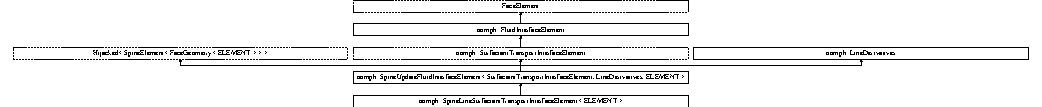
\includegraphics[height=1.435897cm]{classoomph_1_1SpineLineSurfactantTransportInterfaceElement}
\end{center}
\end{figure}
\subsection*{Public Member Functions}
\begin{DoxyCompactItemize}
\item 
\hyperlink{classoomph_1_1SpineLineSurfactantTransportInterfaceElement_a0b9ae72a734043e18ef9fc55629de3b6}{Spine\+Line\+Surfactant\+Transport\+Interface\+Element} (Finite\+Element $\ast$const \&element\+\_\+pt, const int \&face\+\_\+index)
\end{DoxyCompactItemize}
\subsection*{Additional Inherited Members}


\subsection{Detailed Description}
\subsubsection*{template$<$class E\+L\+E\+M\+E\+NT$>$\newline
class oomph\+::\+Spine\+Line\+Surfactant\+Transport\+Interface\+Element$<$ E\+L\+E\+M\+E\+N\+T $>$}

Specialise to the Line geometry. 

Definition at line 202 of file surfactant\+\_\+transport\+\_\+elements.\+h.



\subsection{Constructor \& Destructor Documentation}
\mbox{\Hypertarget{classoomph_1_1SpineLineSurfactantTransportInterfaceElement_a0b9ae72a734043e18ef9fc55629de3b6}\label{classoomph_1_1SpineLineSurfactantTransportInterfaceElement_a0b9ae72a734043e18ef9fc55629de3b6}} 
\index{oomph\+::\+Spine\+Line\+Surfactant\+Transport\+Interface\+Element@{oomph\+::\+Spine\+Line\+Surfactant\+Transport\+Interface\+Element}!Spine\+Line\+Surfactant\+Transport\+Interface\+Element@{Spine\+Line\+Surfactant\+Transport\+Interface\+Element}}
\index{Spine\+Line\+Surfactant\+Transport\+Interface\+Element@{Spine\+Line\+Surfactant\+Transport\+Interface\+Element}!oomph\+::\+Spine\+Line\+Surfactant\+Transport\+Interface\+Element@{oomph\+::\+Spine\+Line\+Surfactant\+Transport\+Interface\+Element}}
\subsubsection{\texorpdfstring{Spine\+Line\+Surfactant\+Transport\+Interface\+Element()}{SpineLineSurfactantTransportInterfaceElement()}}
{\footnotesize\ttfamily template$<$class E\+L\+E\+M\+E\+NT $>$ \\
\hyperlink{classoomph_1_1SpineLineSurfactantTransportInterfaceElement}{oomph\+::\+Spine\+Line\+Surfactant\+Transport\+Interface\+Element}$<$ E\+L\+E\+M\+E\+NT $>$\+::\hyperlink{classoomph_1_1SpineLineSurfactantTransportInterfaceElement}{Spine\+Line\+Surfactant\+Transport\+Interface\+Element} (\begin{DoxyParamCaption}\item[{Finite\+Element $\ast$const \&}]{element\+\_\+pt,  }\item[{const int \&}]{face\+\_\+index }\end{DoxyParamCaption})\hspace{0.3cm}{\ttfamily [inline]}}



Definition at line 208 of file surfactant\+\_\+transport\+\_\+elements.\+h.



The documentation for this class was generated from the following file\+:\begin{DoxyCompactItemize}
\item 
\hyperlink{surfactant__transport__elements_8h}{surfactant\+\_\+transport\+\_\+elements.\+h}\end{DoxyCompactItemize}

\hypertarget{classoomph_1_1SpineLineVolumeConstraintBoundingElement}{}\section{oomph\+:\+:Spine\+Line\+Volume\+Constraint\+Bounding\+Element$<$ E\+L\+E\+M\+E\+NT $>$ Class Template Reference}
\label{classoomph_1_1SpineLineVolumeConstraintBoundingElement}\index{oomph\+::\+Spine\+Line\+Volume\+Constraint\+Bounding\+Element$<$ E\+L\+E\+M\+E\+N\+T $>$@{oomph\+::\+Spine\+Line\+Volume\+Constraint\+Bounding\+Element$<$ E\+L\+E\+M\+E\+N\+T $>$}}


{\ttfamily \#include $<$constrained\+\_\+volume\+\_\+elements.\+h$>$}

Inheritance diagram for oomph\+:\+:Spine\+Line\+Volume\+Constraint\+Bounding\+Element$<$ E\+L\+E\+M\+E\+NT $>$\+:\begin{figure}[H]
\begin{center}
\leavevmode
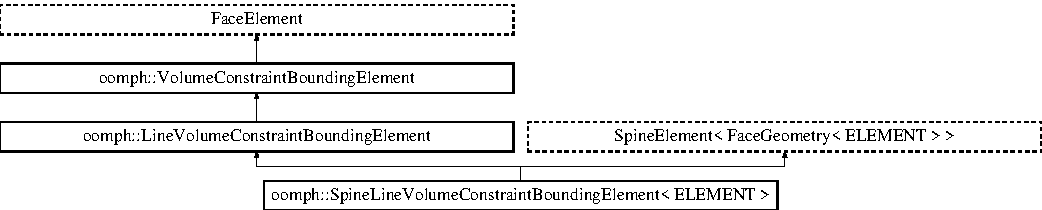
\includegraphics[height=2.821159cm]{classoomph_1_1SpineLineVolumeConstraintBoundingElement}
\end{center}
\end{figure}
\subsection*{Public Member Functions}
\begin{DoxyCompactItemize}
\item 
\hyperlink{classoomph_1_1SpineLineVolumeConstraintBoundingElement_a5b8bb4a60ee78615103eb6b9fa3eb397}{Spine\+Line\+Volume\+Constraint\+Bounding\+Element} (Finite\+Element $\ast$const \&element\+\_\+pt, const int \&face\+\_\+index)
\begin{DoxyCompactList}\small\item\em Contructor\+: Specify bulk element and index of face to which this face element is to be attached. \end{DoxyCompactList}\item 
void \hyperlink{classoomph_1_1SpineLineVolumeConstraintBoundingElement_a9b23d5b98dc459a918045d2a8e221728}{fill\+\_\+in\+\_\+contribution\+\_\+to\+\_\+jacobian} (Vector$<$ double $>$ \&residuals, Dense\+Matrix$<$ double $>$ \&jacobian)
\item 
double \hyperlink{classoomph_1_1SpineLineVolumeConstraintBoundingElement_ab299a1b0cec3d35f5bd6ef683a244db6}{zeta\+\_\+nodal} (const unsigned \&n, const unsigned \&k, const unsigned \&i) const
\begin{DoxyCompactList}\small\item\em The \char`\"{}global\char`\"{} intrinsic coordinate of the element when viewed as part of a geometric object should be given by the Face\+Element representation, by default. \end{DoxyCompactList}\end{DoxyCompactItemize}
\subsection*{Additional Inherited Members}


\subsection{Detailed Description}
\subsubsection*{template$<$class E\+L\+E\+M\+E\+NT$>$\newline
class oomph\+::\+Spine\+Line\+Volume\+Constraint\+Bounding\+Element$<$ E\+L\+E\+M\+E\+N\+T $>$}

The one-\/dimensional interface elements that allow imposition of a volume constraint specialised for the case when the nodal positions of the bulk elements are adjusted using Spines. To enforce that a fluid volume has a certain volume, attach these elements to all faces of the (2D cartesian) bulk fluid elements (of type E\+L\+E\+M\+E\+NT) that bound that region and then specify the \char`\"{}pressure\char`\"{} value that is traded for the constraint. 

Definition at line 433 of file constrained\+\_\+volume\+\_\+elements.\+h.



\subsection{Constructor \& Destructor Documentation}
\mbox{\Hypertarget{classoomph_1_1SpineLineVolumeConstraintBoundingElement_a5b8bb4a60ee78615103eb6b9fa3eb397}\label{classoomph_1_1SpineLineVolumeConstraintBoundingElement_a5b8bb4a60ee78615103eb6b9fa3eb397}} 
\index{oomph\+::\+Spine\+Line\+Volume\+Constraint\+Bounding\+Element@{oomph\+::\+Spine\+Line\+Volume\+Constraint\+Bounding\+Element}!Spine\+Line\+Volume\+Constraint\+Bounding\+Element@{Spine\+Line\+Volume\+Constraint\+Bounding\+Element}}
\index{Spine\+Line\+Volume\+Constraint\+Bounding\+Element@{Spine\+Line\+Volume\+Constraint\+Bounding\+Element}!oomph\+::\+Spine\+Line\+Volume\+Constraint\+Bounding\+Element@{oomph\+::\+Spine\+Line\+Volume\+Constraint\+Bounding\+Element}}
\subsubsection{\texorpdfstring{Spine\+Line\+Volume\+Constraint\+Bounding\+Element()}{SpineLineVolumeConstraintBoundingElement()}}
{\footnotesize\ttfamily template$<$class E\+L\+E\+M\+E\+NT $>$ \\
\hyperlink{classoomph_1_1SpineLineVolumeConstraintBoundingElement}{oomph\+::\+Spine\+Line\+Volume\+Constraint\+Bounding\+Element}$<$ E\+L\+E\+M\+E\+NT $>$\+::\hyperlink{classoomph_1_1SpineLineVolumeConstraintBoundingElement}{Spine\+Line\+Volume\+Constraint\+Bounding\+Element} (\begin{DoxyParamCaption}\item[{Finite\+Element $\ast$const \&}]{element\+\_\+pt,  }\item[{const int \&}]{face\+\_\+index }\end{DoxyParamCaption})\hspace{0.3cm}{\ttfamily [inline]}}



Contructor\+: Specify bulk element and index of face to which this face element is to be attached. 



Definition at line 442 of file constrained\+\_\+volume\+\_\+elements.\+h.



\subsection{Member Function Documentation}
\mbox{\Hypertarget{classoomph_1_1SpineLineVolumeConstraintBoundingElement_a9b23d5b98dc459a918045d2a8e221728}\label{classoomph_1_1SpineLineVolumeConstraintBoundingElement_a9b23d5b98dc459a918045d2a8e221728}} 
\index{oomph\+::\+Spine\+Line\+Volume\+Constraint\+Bounding\+Element@{oomph\+::\+Spine\+Line\+Volume\+Constraint\+Bounding\+Element}!fill\+\_\+in\+\_\+contribution\+\_\+to\+\_\+jacobian@{fill\+\_\+in\+\_\+contribution\+\_\+to\+\_\+jacobian}}
\index{fill\+\_\+in\+\_\+contribution\+\_\+to\+\_\+jacobian@{fill\+\_\+in\+\_\+contribution\+\_\+to\+\_\+jacobian}!oomph\+::\+Spine\+Line\+Volume\+Constraint\+Bounding\+Element@{oomph\+::\+Spine\+Line\+Volume\+Constraint\+Bounding\+Element}}
\subsubsection{\texorpdfstring{fill\+\_\+in\+\_\+contribution\+\_\+to\+\_\+jacobian()}{fill\_in\_contribution\_to\_jacobian()}}
{\footnotesize\ttfamily template$<$class E\+L\+E\+M\+E\+NT $>$ \\
void \hyperlink{classoomph_1_1SpineLineVolumeConstraintBoundingElement}{oomph\+::\+Spine\+Line\+Volume\+Constraint\+Bounding\+Element}$<$ E\+L\+E\+M\+E\+NT $>$\+::fill\+\_\+in\+\_\+contribution\+\_\+to\+\_\+jacobian (\begin{DoxyParamCaption}\item[{Vector$<$ double $>$ \&}]{residuals,  }\item[{Dense\+Matrix$<$ double $>$ \&}]{jacobian }\end{DoxyParamCaption})\hspace{0.3cm}{\ttfamily [inline]}}

Fill in contribution to residuals and Jacobian. This is specific to spine based elements in which the shape derivatives are evaluated using geometric data 

Definition at line 456 of file constrained\+\_\+volume\+\_\+elements.\+h.

\mbox{\Hypertarget{classoomph_1_1SpineLineVolumeConstraintBoundingElement_ab299a1b0cec3d35f5bd6ef683a244db6}\label{classoomph_1_1SpineLineVolumeConstraintBoundingElement_ab299a1b0cec3d35f5bd6ef683a244db6}} 
\index{oomph\+::\+Spine\+Line\+Volume\+Constraint\+Bounding\+Element@{oomph\+::\+Spine\+Line\+Volume\+Constraint\+Bounding\+Element}!zeta\+\_\+nodal@{zeta\+\_\+nodal}}
\index{zeta\+\_\+nodal@{zeta\+\_\+nodal}!oomph\+::\+Spine\+Line\+Volume\+Constraint\+Bounding\+Element@{oomph\+::\+Spine\+Line\+Volume\+Constraint\+Bounding\+Element}}
\subsubsection{\texorpdfstring{zeta\+\_\+nodal()}{zeta\_nodal()}}
{\footnotesize\ttfamily template$<$class E\+L\+E\+M\+E\+NT $>$ \\
double \hyperlink{classoomph_1_1SpineLineVolumeConstraintBoundingElement}{oomph\+::\+Spine\+Line\+Volume\+Constraint\+Bounding\+Element}$<$ E\+L\+E\+M\+E\+NT $>$\+::zeta\+\_\+nodal (\begin{DoxyParamCaption}\item[{const unsigned \&}]{n,  }\item[{const unsigned \&}]{k,  }\item[{const unsigned \&}]{i }\end{DoxyParamCaption}) const\hspace{0.3cm}{\ttfamily [inline]}}



The \char`\"{}global\char`\"{} intrinsic coordinate of the element when viewed as part of a geometric object should be given by the Face\+Element representation, by default. 



Definition at line 469 of file constrained\+\_\+volume\+\_\+elements.\+h.



The documentation for this class was generated from the following file\+:\begin{DoxyCompactItemize}
\item 
\hyperlink{constrained__volume__elements_8h}{constrained\+\_\+volume\+\_\+elements.\+h}\end{DoxyCompactItemize}

\hypertarget{classoomph_1_1SpinePointFluidInterfaceBoundingElement}{}\section{oomph\+:\+:Spine\+Point\+Fluid\+Interface\+Bounding\+Element$<$ E\+L\+E\+M\+E\+NT $>$ Class Template Reference}
\label{classoomph_1_1SpinePointFluidInterfaceBoundingElement}\index{oomph\+::\+Spine\+Point\+Fluid\+Interface\+Bounding\+Element$<$ E\+L\+E\+M\+E\+N\+T $>$@{oomph\+::\+Spine\+Point\+Fluid\+Interface\+Bounding\+Element$<$ E\+L\+E\+M\+E\+N\+T $>$}}


\hyperlink{classoomph_1_1Spine}{Spine} version of the \hyperlink{classoomph_1_1PointFluidInterfaceBoundingElement}{Point\+Fluid\+Interface\+Bounding\+Element}.  




{\ttfamily \#include $<$specific\+\_\+node\+\_\+update\+\_\+interface\+\_\+elements.\+h$>$}

Inheritance diagram for oomph\+:\+:Spine\+Point\+Fluid\+Interface\+Bounding\+Element$<$ E\+L\+E\+M\+E\+NT $>$\+:\begin{figure}[H]
\begin{center}
\leavevmode
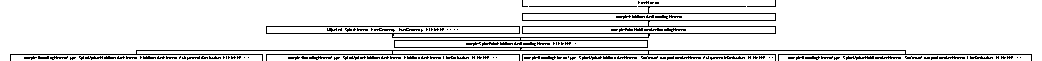
\includegraphics[height=1.055359cm]{classoomph_1_1SpinePointFluidInterfaceBoundingElement}
\end{center}
\end{figure}
\subsection*{Public Member Functions}
\begin{DoxyCompactItemize}
\item 
\hyperlink{classoomph_1_1SpinePointFluidInterfaceBoundingElement_a4cda221f4ee0528cc89076809f54c64e}{Spine\+Point\+Fluid\+Interface\+Bounding\+Element} ()
\begin{DoxyCompactList}\small\item\em Constructor. \end{DoxyCompactList}\item 
void \hyperlink{classoomph_1_1SpinePointFluidInterfaceBoundingElement_ac35833173407cde9359c8163a0eba35c}{output} (std\+::ostream \&outfile)
\begin{DoxyCompactList}\small\item\em Overload the output function. \end{DoxyCompactList}\item 
void \hyperlink{classoomph_1_1SpinePointFluidInterfaceBoundingElement_a05a5383f07c840e07d8c2279cce80aaa}{output} (std\+::ostream \&outfile, const unsigned \&n\+\_\+plot)
\begin{DoxyCompactList}\small\item\em Output the element. \end{DoxyCompactList}\item 
void \hyperlink{classoomph_1_1SpinePointFluidInterfaceBoundingElement_a2435b4b786ede183808834b4d0c5210c}{output} (F\+I\+LE $\ast$file\+\_\+pt)
\begin{DoxyCompactList}\small\item\em Overload the C-\/style output function. \end{DoxyCompactList}\item 
void \hyperlink{classoomph_1_1SpinePointFluidInterfaceBoundingElement_a75a530620bfa2a983fec2e1c7f801db2}{output} (F\+I\+LE $\ast$file\+\_\+pt, const unsigned \&n\+\_\+plot)
\begin{DoxyCompactList}\small\item\em C-\/style Output function. \end{DoxyCompactList}\item 
void \hyperlink{classoomph_1_1SpinePointFluidInterfaceBoundingElement_afe714a2a2b9f741558376cc144e19232}{fill\+\_\+in\+\_\+contribution\+\_\+to\+\_\+jacobian} (\hyperlink{classoomph_1_1Vector}{Vector}$<$ double $>$ \&residuals, \hyperlink{classoomph_1_1DenseMatrix}{Dense\+Matrix}$<$ double $>$ \&jacobian)
\begin{DoxyCompactList}\small\item\em Calculate the elemental residual vector and the Jacobian. \end{DoxyCompactList}\item 
int \hyperlink{classoomph_1_1SpinePointFluidInterfaceBoundingElement_a7c1c2f31b1d9f9c925889ad199a78947}{kinematic\+\_\+local\+\_\+eqn} (const unsigned \&n)
\begin{DoxyCompactList}\small\item\em Return local equation number associated with the kinematic constraint for local node n. \end{DoxyCompactList}\end{DoxyCompactItemize}
\subsection*{Additional Inherited Members}


\subsection{Detailed Description}
\subsubsection*{template$<$class E\+L\+E\+M\+E\+NT$>$\newline
class oomph\+::\+Spine\+Point\+Fluid\+Interface\+Bounding\+Element$<$ E\+L\+E\+M\+E\+N\+T $>$}

\hyperlink{classoomph_1_1Spine}{Spine} version of the \hyperlink{classoomph_1_1PointFluidInterfaceBoundingElement}{Point\+Fluid\+Interface\+Bounding\+Element}. 

Definition at line 384 of file specific\+\_\+node\+\_\+update\+\_\+interface\+\_\+elements.\+h.



\subsection{Constructor \& Destructor Documentation}
\mbox{\Hypertarget{classoomph_1_1SpinePointFluidInterfaceBoundingElement_a4cda221f4ee0528cc89076809f54c64e}\label{classoomph_1_1SpinePointFluidInterfaceBoundingElement_a4cda221f4ee0528cc89076809f54c64e}} 
\index{oomph\+::\+Spine\+Point\+Fluid\+Interface\+Bounding\+Element@{oomph\+::\+Spine\+Point\+Fluid\+Interface\+Bounding\+Element}!Spine\+Point\+Fluid\+Interface\+Bounding\+Element@{Spine\+Point\+Fluid\+Interface\+Bounding\+Element}}
\index{Spine\+Point\+Fluid\+Interface\+Bounding\+Element@{Spine\+Point\+Fluid\+Interface\+Bounding\+Element}!oomph\+::\+Spine\+Point\+Fluid\+Interface\+Bounding\+Element@{oomph\+::\+Spine\+Point\+Fluid\+Interface\+Bounding\+Element}}
\subsubsection{\texorpdfstring{Spine\+Point\+Fluid\+Interface\+Bounding\+Element()}{SpinePointFluidInterfaceBoundingElement()}}
{\footnotesize\ttfamily template$<$class E\+L\+E\+M\+E\+NT $>$ \\
\hyperlink{classoomph_1_1SpinePointFluidInterfaceBoundingElement}{oomph\+::\+Spine\+Point\+Fluid\+Interface\+Bounding\+Element}$<$ E\+L\+E\+M\+E\+NT $>$\+::\hyperlink{classoomph_1_1SpinePointFluidInterfaceBoundingElement}{Spine\+Point\+Fluid\+Interface\+Bounding\+Element} (\begin{DoxyParamCaption}{ }\end{DoxyParamCaption})\hspace{0.3cm}{\ttfamily [inline]}}



Constructor. 



Definition at line 393 of file specific\+\_\+node\+\_\+update\+\_\+interface\+\_\+elements.\+h.



\subsection{Member Function Documentation}
\mbox{\Hypertarget{classoomph_1_1SpinePointFluidInterfaceBoundingElement_afe714a2a2b9f741558376cc144e19232}\label{classoomph_1_1SpinePointFluidInterfaceBoundingElement_afe714a2a2b9f741558376cc144e19232}} 
\index{oomph\+::\+Spine\+Point\+Fluid\+Interface\+Bounding\+Element@{oomph\+::\+Spine\+Point\+Fluid\+Interface\+Bounding\+Element}!fill\+\_\+in\+\_\+contribution\+\_\+to\+\_\+jacobian@{fill\+\_\+in\+\_\+contribution\+\_\+to\+\_\+jacobian}}
\index{fill\+\_\+in\+\_\+contribution\+\_\+to\+\_\+jacobian@{fill\+\_\+in\+\_\+contribution\+\_\+to\+\_\+jacobian}!oomph\+::\+Spine\+Point\+Fluid\+Interface\+Bounding\+Element@{oomph\+::\+Spine\+Point\+Fluid\+Interface\+Bounding\+Element}}
\subsubsection{\texorpdfstring{fill\+\_\+in\+\_\+contribution\+\_\+to\+\_\+jacobian()}{fill\_in\_contribution\_to\_jacobian()}}
{\footnotesize\ttfamily template$<$class E\+L\+E\+M\+E\+NT $>$ \\
void \hyperlink{classoomph_1_1SpinePointFluidInterfaceBoundingElement}{oomph\+::\+Spine\+Point\+Fluid\+Interface\+Bounding\+Element}$<$ E\+L\+E\+M\+E\+NT $>$\+::fill\+\_\+in\+\_\+contribution\+\_\+to\+\_\+jacobian (\begin{DoxyParamCaption}\item[{\hyperlink{classoomph_1_1Vector}{Vector}$<$ double $>$ \&}]{residuals,  }\item[{\hyperlink{classoomph_1_1DenseMatrix}{Dense\+Matrix}$<$ double $>$ \&}]{jacobian }\end{DoxyParamCaption})\hspace{0.3cm}{\ttfamily [inline]}, {\ttfamily [virtual]}}



Calculate the elemental residual vector and the Jacobian. 



Reimplemented from \hyperlink{classoomph_1_1GeneralisedElement_a6ae09fc0d68e4309ac1b03583d252845}{oomph\+::\+Generalised\+Element}.



Definition at line 412 of file specific\+\_\+node\+\_\+update\+\_\+interface\+\_\+elements.\+h.

\mbox{\Hypertarget{classoomph_1_1SpinePointFluidInterfaceBoundingElement_a7c1c2f31b1d9f9c925889ad199a78947}\label{classoomph_1_1SpinePointFluidInterfaceBoundingElement_a7c1c2f31b1d9f9c925889ad199a78947}} 
\index{oomph\+::\+Spine\+Point\+Fluid\+Interface\+Bounding\+Element@{oomph\+::\+Spine\+Point\+Fluid\+Interface\+Bounding\+Element}!kinematic\+\_\+local\+\_\+eqn@{kinematic\+\_\+local\+\_\+eqn}}
\index{kinematic\+\_\+local\+\_\+eqn@{kinematic\+\_\+local\+\_\+eqn}!oomph\+::\+Spine\+Point\+Fluid\+Interface\+Bounding\+Element@{oomph\+::\+Spine\+Point\+Fluid\+Interface\+Bounding\+Element}}
\subsubsection{\texorpdfstring{kinematic\+\_\+local\+\_\+eqn()}{kinematic\_local\_eqn()}}
{\footnotesize\ttfamily template$<$class E\+L\+E\+M\+E\+NT $>$ \\
int \hyperlink{classoomph_1_1SpinePointFluidInterfaceBoundingElement}{oomph\+::\+Spine\+Point\+Fluid\+Interface\+Bounding\+Element}$<$ E\+L\+E\+M\+E\+NT $>$\+::kinematic\+\_\+local\+\_\+eqn (\begin{DoxyParamCaption}\item[{const unsigned \&}]{n }\end{DoxyParamCaption})\hspace{0.3cm}{\ttfamily [inline]}, {\ttfamily [virtual]}}



Return local equation number associated with the kinematic constraint for local node n. 



Implements \hyperlink{classoomph_1_1FluidInterfaceBoundingElement_a12a0a6d7c3c1c1a5a0f42a57e60eab34}{oomph\+::\+Fluid\+Interface\+Bounding\+Element}.



Definition at line 427 of file specific\+\_\+node\+\_\+update\+\_\+interface\+\_\+elements.\+h.

\mbox{\Hypertarget{classoomph_1_1SpinePointFluidInterfaceBoundingElement_ac35833173407cde9359c8163a0eba35c}\label{classoomph_1_1SpinePointFluidInterfaceBoundingElement_ac35833173407cde9359c8163a0eba35c}} 
\index{oomph\+::\+Spine\+Point\+Fluid\+Interface\+Bounding\+Element@{oomph\+::\+Spine\+Point\+Fluid\+Interface\+Bounding\+Element}!output@{output}}
\index{output@{output}!oomph\+::\+Spine\+Point\+Fluid\+Interface\+Bounding\+Element@{oomph\+::\+Spine\+Point\+Fluid\+Interface\+Bounding\+Element}}
\subsubsection{\texorpdfstring{output()}{output()}\hspace{0.1cm}{\footnotesize\ttfamily [1/4]}}
{\footnotesize\ttfamily template$<$class E\+L\+E\+M\+E\+NT $>$ \\
void \hyperlink{classoomph_1_1SpinePointFluidInterfaceBoundingElement}{oomph\+::\+Spine\+Point\+Fluid\+Interface\+Bounding\+Element}$<$ E\+L\+E\+M\+E\+NT $>$\+::output (\begin{DoxyParamCaption}\item[{std\+::ostream \&}]{outfile }\end{DoxyParamCaption})\hspace{0.3cm}{\ttfamily [inline]}, {\ttfamily [virtual]}}



Overload the output function. 



Reimplemented from \hyperlink{classoomph_1_1FluidInterfaceBoundingElement_a81adc5ae89ddfa120f587c61b972622f}{oomph\+::\+Fluid\+Interface\+Bounding\+Element}.



Definition at line 398 of file specific\+\_\+node\+\_\+update\+\_\+interface\+\_\+elements.\+h.



References oomph\+::\+Finite\+Element\+::output().

\mbox{\Hypertarget{classoomph_1_1SpinePointFluidInterfaceBoundingElement_a05a5383f07c840e07d8c2279cce80aaa}\label{classoomph_1_1SpinePointFluidInterfaceBoundingElement_a05a5383f07c840e07d8c2279cce80aaa}} 
\index{oomph\+::\+Spine\+Point\+Fluid\+Interface\+Bounding\+Element@{oomph\+::\+Spine\+Point\+Fluid\+Interface\+Bounding\+Element}!output@{output}}
\index{output@{output}!oomph\+::\+Spine\+Point\+Fluid\+Interface\+Bounding\+Element@{oomph\+::\+Spine\+Point\+Fluid\+Interface\+Bounding\+Element}}
\subsubsection{\texorpdfstring{output()}{output()}\hspace{0.1cm}{\footnotesize\ttfamily [2/4]}}
{\footnotesize\ttfamily template$<$class E\+L\+E\+M\+E\+NT $>$ \\
void \hyperlink{classoomph_1_1SpinePointFluidInterfaceBoundingElement}{oomph\+::\+Spine\+Point\+Fluid\+Interface\+Bounding\+Element}$<$ E\+L\+E\+M\+E\+NT $>$\+::output (\begin{DoxyParamCaption}\item[{std\+::ostream \&}]{outfile,  }\item[{const unsigned \&}]{n\+\_\+plot }\end{DoxyParamCaption})\hspace{0.3cm}{\ttfamily [inline]}, {\ttfamily [virtual]}}



Output the element. 



Reimplemented from \hyperlink{classoomph_1_1FluidInterfaceBoundingElement_af2c821d51d506221976a0c17e1615ac3}{oomph\+::\+Fluid\+Interface\+Bounding\+Element}.



Definition at line 401 of file specific\+\_\+node\+\_\+update\+\_\+interface\+\_\+elements.\+h.



References oomph\+::\+Fluid\+Interface\+Bounding\+Element\+::output().

\mbox{\Hypertarget{classoomph_1_1SpinePointFluidInterfaceBoundingElement_a2435b4b786ede183808834b4d0c5210c}\label{classoomph_1_1SpinePointFluidInterfaceBoundingElement_a2435b4b786ede183808834b4d0c5210c}} 
\index{oomph\+::\+Spine\+Point\+Fluid\+Interface\+Bounding\+Element@{oomph\+::\+Spine\+Point\+Fluid\+Interface\+Bounding\+Element}!output@{output}}
\index{output@{output}!oomph\+::\+Spine\+Point\+Fluid\+Interface\+Bounding\+Element@{oomph\+::\+Spine\+Point\+Fluid\+Interface\+Bounding\+Element}}
\subsubsection{\texorpdfstring{output()}{output()}\hspace{0.1cm}{\footnotesize\ttfamily [3/4]}}
{\footnotesize\ttfamily template$<$class E\+L\+E\+M\+E\+NT $>$ \\
void \hyperlink{classoomph_1_1SpinePointFluidInterfaceBoundingElement}{oomph\+::\+Spine\+Point\+Fluid\+Interface\+Bounding\+Element}$<$ E\+L\+E\+M\+E\+NT $>$\+::output (\begin{DoxyParamCaption}\item[{F\+I\+LE $\ast$}]{file\+\_\+pt }\end{DoxyParamCaption})\hspace{0.3cm}{\ttfamily [inline]}, {\ttfamily [virtual]}}



Overload the C-\/style output function. 



Reimplemented from \hyperlink{classoomph_1_1FluidInterfaceBoundingElement_a85cc62405429744e3e3585894315cb9e}{oomph\+::\+Fluid\+Interface\+Bounding\+Element}.



Definition at line 405 of file specific\+\_\+node\+\_\+update\+\_\+interface\+\_\+elements.\+h.



References oomph\+::\+Finite\+Element\+::output().

\mbox{\Hypertarget{classoomph_1_1SpinePointFluidInterfaceBoundingElement_a75a530620bfa2a983fec2e1c7f801db2}\label{classoomph_1_1SpinePointFluidInterfaceBoundingElement_a75a530620bfa2a983fec2e1c7f801db2}} 
\index{oomph\+::\+Spine\+Point\+Fluid\+Interface\+Bounding\+Element@{oomph\+::\+Spine\+Point\+Fluid\+Interface\+Bounding\+Element}!output@{output}}
\index{output@{output}!oomph\+::\+Spine\+Point\+Fluid\+Interface\+Bounding\+Element@{oomph\+::\+Spine\+Point\+Fluid\+Interface\+Bounding\+Element}}
\subsubsection{\texorpdfstring{output()}{output()}\hspace{0.1cm}{\footnotesize\ttfamily [4/4]}}
{\footnotesize\ttfamily template$<$class E\+L\+E\+M\+E\+NT $>$ \\
void \hyperlink{classoomph_1_1SpinePointFluidInterfaceBoundingElement}{oomph\+::\+Spine\+Point\+Fluid\+Interface\+Bounding\+Element}$<$ E\+L\+E\+M\+E\+NT $>$\+::output (\begin{DoxyParamCaption}\item[{F\+I\+LE $\ast$}]{file\+\_\+pt,  }\item[{const unsigned \&}]{n\+\_\+plot }\end{DoxyParamCaption})\hspace{0.3cm}{\ttfamily [inline]}, {\ttfamily [virtual]}}



C-\/style Output function. 



Reimplemented from \hyperlink{classoomph_1_1FluidInterfaceBoundingElement_ae85ea987a06275a03ad6d0e3710871da}{oomph\+::\+Fluid\+Interface\+Bounding\+Element}.



Definition at line 408 of file specific\+\_\+node\+\_\+update\+\_\+interface\+\_\+elements.\+h.



References oomph\+::\+Fluid\+Interface\+Bounding\+Element\+::output().



The documentation for this class was generated from the following file\+:\begin{DoxyCompactItemize}
\item 
\hyperlink{specific__node__update__interface__elements_8h}{specific\+\_\+node\+\_\+update\+\_\+interface\+\_\+elements.\+h}\end{DoxyCompactItemize}

\hypertarget{classoomph_1_1SpineSurfaceFluidInterfaceElement}{}\section{oomph\+:\+:Spine\+Surface\+Fluid\+Interface\+Element$<$ E\+L\+E\+M\+E\+NT $>$ Class Template Reference}
\label{classoomph_1_1SpineSurfaceFluidInterfaceElement}\index{oomph\+::\+Spine\+Surface\+Fluid\+Interface\+Element$<$ E\+L\+E\+M\+E\+N\+T $>$@{oomph\+::\+Spine\+Surface\+Fluid\+Interface\+Element$<$ E\+L\+E\+M\+E\+N\+T $>$}}


{\ttfamily \#include $<$specific\+\_\+node\+\_\+update\+\_\+interface\+\_\+elements.\+h$>$}

Inheritance diagram for oomph\+:\+:Spine\+Surface\+Fluid\+Interface\+Element$<$ E\+L\+E\+M\+E\+NT $>$\+:\begin{figure}[H]
\begin{center}
\leavevmode
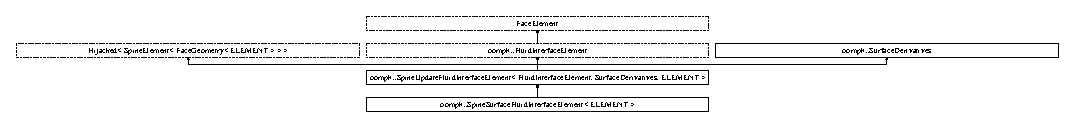
\includegraphics[height=1.272004cm]{classoomph_1_1SpineSurfaceFluidInterfaceElement}
\end{center}
\end{figure}
\subsection*{Public Member Functions}
\begin{DoxyCompactItemize}
\item 
\hyperlink{classoomph_1_1SpineSurfaceFluidInterfaceElement_aa1d52a09e4f50085b957463a0da22d4a}{Spine\+Surface\+Fluid\+Interface\+Element} (Finite\+Element $\ast$const \&element\+\_\+pt, const int \&face\+\_\+index)
\end{DoxyCompactItemize}
\subsection*{Additional Inherited Members}


\subsection{Detailed Description}
\subsubsection*{template$<$class E\+L\+E\+M\+E\+NT$>$\newline
class oomph\+::\+Spine\+Surface\+Fluid\+Interface\+Element$<$ E\+L\+E\+M\+E\+N\+T $>$}



Definition at line 553 of file specific\+\_\+node\+\_\+update\+\_\+interface\+\_\+elements.\+h.



\subsection{Constructor \& Destructor Documentation}
\mbox{\Hypertarget{classoomph_1_1SpineSurfaceFluidInterfaceElement_aa1d52a09e4f50085b957463a0da22d4a}\label{classoomph_1_1SpineSurfaceFluidInterfaceElement_aa1d52a09e4f50085b957463a0da22d4a}} 
\index{oomph\+::\+Spine\+Surface\+Fluid\+Interface\+Element@{oomph\+::\+Spine\+Surface\+Fluid\+Interface\+Element}!Spine\+Surface\+Fluid\+Interface\+Element@{Spine\+Surface\+Fluid\+Interface\+Element}}
\index{Spine\+Surface\+Fluid\+Interface\+Element@{Spine\+Surface\+Fluid\+Interface\+Element}!oomph\+::\+Spine\+Surface\+Fluid\+Interface\+Element@{oomph\+::\+Spine\+Surface\+Fluid\+Interface\+Element}}
\subsubsection{\texorpdfstring{Spine\+Surface\+Fluid\+Interface\+Element()}{SpineSurfaceFluidInterfaceElement()}}
{\footnotesize\ttfamily template$<$class E\+L\+E\+M\+E\+NT $>$ \\
\hyperlink{classoomph_1_1SpineSurfaceFluidInterfaceElement}{oomph\+::\+Spine\+Surface\+Fluid\+Interface\+Element}$<$ E\+L\+E\+M\+E\+NT $>$\+::\hyperlink{classoomph_1_1SpineSurfaceFluidInterfaceElement}{Spine\+Surface\+Fluid\+Interface\+Element} (\begin{DoxyParamCaption}\item[{Finite\+Element $\ast$const \&}]{element\+\_\+pt,  }\item[{const int \&}]{face\+\_\+index }\end{DoxyParamCaption})\hspace{0.3cm}{\ttfamily [inline]}}



Definition at line 559 of file specific\+\_\+node\+\_\+update\+\_\+interface\+\_\+elements.\+h.



The documentation for this class was generated from the following file\+:\begin{DoxyCompactItemize}
\item 
\hyperlink{specific__node__update__interface__elements_8h}{specific\+\_\+node\+\_\+update\+\_\+interface\+\_\+elements.\+h}\end{DoxyCompactItemize}

\hypertarget{classoomph_1_1SpineSurfaceSurfactantTransportInterfaceElement}{}\section{oomph\+:\+:Spine\+Surface\+Surfactant\+Transport\+Interface\+Element$<$ E\+L\+E\+M\+E\+NT $>$ Class Template Reference}
\label{classoomph_1_1SpineSurfaceSurfactantTransportInterfaceElement}\index{oomph\+::\+Spine\+Surface\+Surfactant\+Transport\+Interface\+Element$<$ E\+L\+E\+M\+E\+N\+T $>$@{oomph\+::\+Spine\+Surface\+Surfactant\+Transport\+Interface\+Element$<$ E\+L\+E\+M\+E\+N\+T $>$}}


Specialise to surface geometry.  




{\ttfamily \#include $<$surfactant\+\_\+transport\+\_\+elements.\+h$>$}

Inheritance diagram for oomph\+:\+:Spine\+Surface\+Surfactant\+Transport\+Interface\+Element$<$ E\+L\+E\+M\+E\+NT $>$\+:\begin{figure}[H]
\begin{center}
\leavevmode
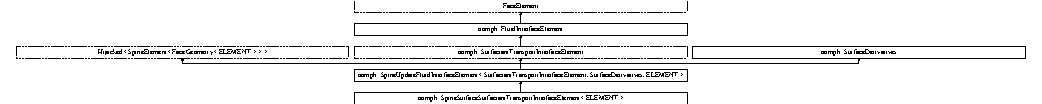
\includegraphics[height=1.390959cm]{classoomph_1_1SpineSurfaceSurfactantTransportInterfaceElement}
\end{center}
\end{figure}
\subsection*{Public Member Functions}
\begin{DoxyCompactItemize}
\item 
\hyperlink{classoomph_1_1SpineSurfaceSurfactantTransportInterfaceElement_aa3014e796ec7e0bfa26824fc42184d06}{Spine\+Surface\+Surfactant\+Transport\+Interface\+Element} (Finite\+Element $\ast$const \&element\+\_\+pt, const int \&face\+\_\+index)
\end{DoxyCompactItemize}
\subsection*{Additional Inherited Members}


\subsection{Detailed Description}
\subsubsection*{template$<$class E\+L\+E\+M\+E\+NT$>$\newline
class oomph\+::\+Spine\+Surface\+Surfactant\+Transport\+Interface\+Element$<$ E\+L\+E\+M\+E\+N\+T $>$}

Specialise to surface geometry. 

Definition at line 291 of file surfactant\+\_\+transport\+\_\+elements.\+h.



\subsection{Constructor \& Destructor Documentation}
\mbox{\Hypertarget{classoomph_1_1SpineSurfaceSurfactantTransportInterfaceElement_aa3014e796ec7e0bfa26824fc42184d06}\label{classoomph_1_1SpineSurfaceSurfactantTransportInterfaceElement_aa3014e796ec7e0bfa26824fc42184d06}} 
\index{oomph\+::\+Spine\+Surface\+Surfactant\+Transport\+Interface\+Element@{oomph\+::\+Spine\+Surface\+Surfactant\+Transport\+Interface\+Element}!Spine\+Surface\+Surfactant\+Transport\+Interface\+Element@{Spine\+Surface\+Surfactant\+Transport\+Interface\+Element}}
\index{Spine\+Surface\+Surfactant\+Transport\+Interface\+Element@{Spine\+Surface\+Surfactant\+Transport\+Interface\+Element}!oomph\+::\+Spine\+Surface\+Surfactant\+Transport\+Interface\+Element@{oomph\+::\+Spine\+Surface\+Surfactant\+Transport\+Interface\+Element}}
\subsubsection{\texorpdfstring{Spine\+Surface\+Surfactant\+Transport\+Interface\+Element()}{SpineSurfaceSurfactantTransportInterfaceElement()}}
{\footnotesize\ttfamily template$<$class E\+L\+E\+M\+E\+NT $>$ \\
\hyperlink{classoomph_1_1SpineSurfaceSurfactantTransportInterfaceElement}{oomph\+::\+Spine\+Surface\+Surfactant\+Transport\+Interface\+Element}$<$ E\+L\+E\+M\+E\+NT $>$\+::\hyperlink{classoomph_1_1SpineSurfaceSurfactantTransportInterfaceElement}{Spine\+Surface\+Surfactant\+Transport\+Interface\+Element} (\begin{DoxyParamCaption}\item[{Finite\+Element $\ast$const \&}]{element\+\_\+pt,  }\item[{const int \&}]{face\+\_\+index }\end{DoxyParamCaption})\hspace{0.3cm}{\ttfamily [inline]}}



Definition at line 297 of file surfactant\+\_\+transport\+\_\+elements.\+h.



The documentation for this class was generated from the following file\+:\begin{DoxyCompactItemize}
\item 
\hyperlink{surfactant__transport__elements_8h}{surfactant\+\_\+transport\+\_\+elements.\+h}\end{DoxyCompactItemize}

\hypertarget{classoomph_1_1SpineSurfaceVolumeConstraintBoundingElement}{}\section{oomph\+:\+:Spine\+Surface\+Volume\+Constraint\+Bounding\+Element$<$ E\+L\+E\+M\+E\+NT $>$ Class Template Reference}
\label{classoomph_1_1SpineSurfaceVolumeConstraintBoundingElement}\index{oomph\+::\+Spine\+Surface\+Volume\+Constraint\+Bounding\+Element$<$ E\+L\+E\+M\+E\+N\+T $>$@{oomph\+::\+Spine\+Surface\+Volume\+Constraint\+Bounding\+Element$<$ E\+L\+E\+M\+E\+N\+T $>$}}


{\ttfamily \#include $<$constrained\+\_\+volume\+\_\+elements.\+h$>$}

Inheritance diagram for oomph\+:\+:Spine\+Surface\+Volume\+Constraint\+Bounding\+Element$<$ E\+L\+E\+M\+E\+NT $>$\+:\begin{figure}[H]
\begin{center}
\leavevmode
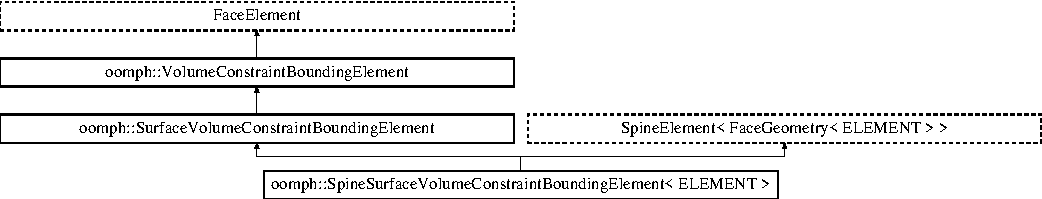
\includegraphics[height=2.679426cm]{classoomph_1_1SpineSurfaceVolumeConstraintBoundingElement}
\end{center}
\end{figure}
\subsection*{Public Member Functions}
\begin{DoxyCompactItemize}
\item 
\hyperlink{classoomph_1_1SpineSurfaceVolumeConstraintBoundingElement_a1426f4750d43008e7c33526cf01f23f3}{Spine\+Surface\+Volume\+Constraint\+Bounding\+Element} (Finite\+Element $\ast$const \&element\+\_\+pt, const int \&face\+\_\+index)
\begin{DoxyCompactList}\small\item\em Contructor\+: Specify bulk element and index of face to which this face element is to be attached. \end{DoxyCompactList}\item 
void \hyperlink{classoomph_1_1SpineSurfaceVolumeConstraintBoundingElement_a5eec2e025f24120c6f2a959da70bb5b1}{fill\+\_\+in\+\_\+contribution\+\_\+to\+\_\+jacobian} (Vector$<$ double $>$ \&residuals, Dense\+Matrix$<$ double $>$ \&jacobian)
\item 
double \hyperlink{classoomph_1_1SpineSurfaceVolumeConstraintBoundingElement_aa252629ad8c455a83b5f2e9643a36e94}{zeta\+\_\+nodal} (const unsigned \&n, const unsigned \&k, const unsigned \&i) const
\begin{DoxyCompactList}\small\item\em The \char`\"{}global\char`\"{} intrinsic coordinate of the element when viewed as part of a geometric object should be given by the Face\+Element representation, by default. \end{DoxyCompactList}\end{DoxyCompactItemize}
\subsection*{Additional Inherited Members}


\subsection{Detailed Description}
\subsubsection*{template$<$class E\+L\+E\+M\+E\+NT$>$\newline
class oomph\+::\+Spine\+Surface\+Volume\+Constraint\+Bounding\+Element$<$ E\+L\+E\+M\+E\+N\+T $>$}

The Two-\/dimensional interface elements that allow the application of a volume constraint specialised for the case when the nodal positions of the bulk elements are adjusted using spines. To enforce that a fluid volume has a certain volume, attach these elements to all faces of the (3D Cartesian) bulk fluid elements (of type E\+L\+E\+M\+E\+NT) that bound that region and then specify the \char`\"{}pressure\char`\"{} value that is traded for the constraint. 

Definition at line 829 of file constrained\+\_\+volume\+\_\+elements.\+h.



\subsection{Constructor \& Destructor Documentation}
\mbox{\Hypertarget{classoomph_1_1SpineSurfaceVolumeConstraintBoundingElement_a1426f4750d43008e7c33526cf01f23f3}\label{classoomph_1_1SpineSurfaceVolumeConstraintBoundingElement_a1426f4750d43008e7c33526cf01f23f3}} 
\index{oomph\+::\+Spine\+Surface\+Volume\+Constraint\+Bounding\+Element@{oomph\+::\+Spine\+Surface\+Volume\+Constraint\+Bounding\+Element}!Spine\+Surface\+Volume\+Constraint\+Bounding\+Element@{Spine\+Surface\+Volume\+Constraint\+Bounding\+Element}}
\index{Spine\+Surface\+Volume\+Constraint\+Bounding\+Element@{Spine\+Surface\+Volume\+Constraint\+Bounding\+Element}!oomph\+::\+Spine\+Surface\+Volume\+Constraint\+Bounding\+Element@{oomph\+::\+Spine\+Surface\+Volume\+Constraint\+Bounding\+Element}}
\subsubsection{\texorpdfstring{Spine\+Surface\+Volume\+Constraint\+Bounding\+Element()}{SpineSurfaceVolumeConstraintBoundingElement()}}
{\footnotesize\ttfamily template$<$class E\+L\+E\+M\+E\+NT $>$ \\
\hyperlink{classoomph_1_1SpineSurfaceVolumeConstraintBoundingElement}{oomph\+::\+Spine\+Surface\+Volume\+Constraint\+Bounding\+Element}$<$ E\+L\+E\+M\+E\+NT $>$\+::\hyperlink{classoomph_1_1SpineSurfaceVolumeConstraintBoundingElement}{Spine\+Surface\+Volume\+Constraint\+Bounding\+Element} (\begin{DoxyParamCaption}\item[{Finite\+Element $\ast$const \&}]{element\+\_\+pt,  }\item[{const int \&}]{face\+\_\+index }\end{DoxyParamCaption})\hspace{0.3cm}{\ttfamily [inline]}}



Contructor\+: Specify bulk element and index of face to which this face element is to be attached. 



Definition at line 838 of file constrained\+\_\+volume\+\_\+elements.\+h.



\subsection{Member Function Documentation}
\mbox{\Hypertarget{classoomph_1_1SpineSurfaceVolumeConstraintBoundingElement_a5eec2e025f24120c6f2a959da70bb5b1}\label{classoomph_1_1SpineSurfaceVolumeConstraintBoundingElement_a5eec2e025f24120c6f2a959da70bb5b1}} 
\index{oomph\+::\+Spine\+Surface\+Volume\+Constraint\+Bounding\+Element@{oomph\+::\+Spine\+Surface\+Volume\+Constraint\+Bounding\+Element}!fill\+\_\+in\+\_\+contribution\+\_\+to\+\_\+jacobian@{fill\+\_\+in\+\_\+contribution\+\_\+to\+\_\+jacobian}}
\index{fill\+\_\+in\+\_\+contribution\+\_\+to\+\_\+jacobian@{fill\+\_\+in\+\_\+contribution\+\_\+to\+\_\+jacobian}!oomph\+::\+Spine\+Surface\+Volume\+Constraint\+Bounding\+Element@{oomph\+::\+Spine\+Surface\+Volume\+Constraint\+Bounding\+Element}}
\subsubsection{\texorpdfstring{fill\+\_\+in\+\_\+contribution\+\_\+to\+\_\+jacobian()}{fill\_in\_contribution\_to\_jacobian()}}
{\footnotesize\ttfamily template$<$class E\+L\+E\+M\+E\+NT $>$ \\
void \hyperlink{classoomph_1_1SpineSurfaceVolumeConstraintBoundingElement}{oomph\+::\+Spine\+Surface\+Volume\+Constraint\+Bounding\+Element}$<$ E\+L\+E\+M\+E\+NT $>$\+::fill\+\_\+in\+\_\+contribution\+\_\+to\+\_\+jacobian (\begin{DoxyParamCaption}\item[{Vector$<$ double $>$ \&}]{residuals,  }\item[{Dense\+Matrix$<$ double $>$ \&}]{jacobian }\end{DoxyParamCaption})\hspace{0.3cm}{\ttfamily [inline]}}

Fill in contribution to residuals and Jacobian. This is specific to spine based elements in which the shape derivatives are evaluated using geometric data 

Definition at line 853 of file constrained\+\_\+volume\+\_\+elements.\+h.

\mbox{\Hypertarget{classoomph_1_1SpineSurfaceVolumeConstraintBoundingElement_aa252629ad8c455a83b5f2e9643a36e94}\label{classoomph_1_1SpineSurfaceVolumeConstraintBoundingElement_aa252629ad8c455a83b5f2e9643a36e94}} 
\index{oomph\+::\+Spine\+Surface\+Volume\+Constraint\+Bounding\+Element@{oomph\+::\+Spine\+Surface\+Volume\+Constraint\+Bounding\+Element}!zeta\+\_\+nodal@{zeta\+\_\+nodal}}
\index{zeta\+\_\+nodal@{zeta\+\_\+nodal}!oomph\+::\+Spine\+Surface\+Volume\+Constraint\+Bounding\+Element@{oomph\+::\+Spine\+Surface\+Volume\+Constraint\+Bounding\+Element}}
\subsubsection{\texorpdfstring{zeta\+\_\+nodal()}{zeta\_nodal()}}
{\footnotesize\ttfamily template$<$class E\+L\+E\+M\+E\+NT $>$ \\
double \hyperlink{classoomph_1_1SpineSurfaceVolumeConstraintBoundingElement}{oomph\+::\+Spine\+Surface\+Volume\+Constraint\+Bounding\+Element}$<$ E\+L\+E\+M\+E\+NT $>$\+::zeta\+\_\+nodal (\begin{DoxyParamCaption}\item[{const unsigned \&}]{n,  }\item[{const unsigned \&}]{k,  }\item[{const unsigned \&}]{i }\end{DoxyParamCaption}) const\hspace{0.3cm}{\ttfamily [inline]}}



The \char`\"{}global\char`\"{} intrinsic coordinate of the element when viewed as part of a geometric object should be given by the Face\+Element representation, by default. 



Definition at line 867 of file constrained\+\_\+volume\+\_\+elements.\+h.



The documentation for this class was generated from the following file\+:\begin{DoxyCompactItemize}
\item 
\hyperlink{constrained__volume__elements_8h}{constrained\+\_\+volume\+\_\+elements.\+h}\end{DoxyCompactItemize}

\hypertarget{classoomph_1_1SpineUpdateFluidInterfaceElement}{}\section{oomph\+:\+:Spine\+Update\+Fluid\+Interface\+Element$<$ E\+Q\+U\+A\+T\+I\+O\+N\+\_\+\+C\+L\+A\+SS, D\+E\+R\+I\+V\+A\+T\+I\+V\+E\+\_\+\+C\+L\+A\+SS, E\+L\+E\+M\+E\+NT $>$ Class Template Reference}
\label{classoomph_1_1SpineUpdateFluidInterfaceElement}\index{oomph\+::\+Spine\+Update\+Fluid\+Interface\+Element$<$ E\+Q\+U\+A\+T\+I\+O\+N\+\_\+\+C\+L\+A\+S\+S, D\+E\+R\+I\+V\+A\+T\+I\+V\+E\+\_\+\+C\+L\+A\+S\+S, E\+L\+E\+M\+E\+N\+T $>$@{oomph\+::\+Spine\+Update\+Fluid\+Interface\+Element$<$ E\+Q\+U\+A\+T\+I\+O\+N\+\_\+\+C\+L\+A\+S\+S, D\+E\+R\+I\+V\+A\+T\+I\+V\+E\+\_\+\+C\+L\+A\+S\+S, E\+L\+E\+M\+E\+N\+T $>$}}


Generic \hyperlink{classoomph_1_1Spine}{Spine} node update interface template class that can be combined with a given surface equations class and surface derivative class to provide a concrete implementation of any surface element that uses spines.  




{\ttfamily \#include $<$specific\+\_\+node\+\_\+update\+\_\+interface\+\_\+elements.\+h$>$}

Inheritance diagram for oomph\+:\+:Spine\+Update\+Fluid\+Interface\+Element$<$ E\+Q\+U\+A\+T\+I\+O\+N\+\_\+\+C\+L\+A\+SS, D\+E\+R\+I\+V\+A\+T\+I\+V\+E\+\_\+\+C\+L\+A\+SS, E\+L\+E\+M\+E\+NT $>$\+:\begin{figure}[H]
\begin{center}
\leavevmode
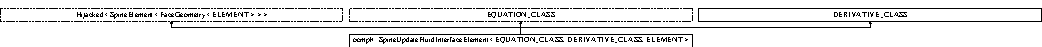
\includegraphics[height=1.331070cm]{classoomph_1_1SpineUpdateFluidInterfaceElement}
\end{center}
\end{figure}
\subsection*{Public Member Functions}
\begin{DoxyCompactItemize}
\item 
\hyperlink{classoomph_1_1SpineUpdateFluidInterfaceElement_a2cc44705997f9fb44abf56ddb5f0cde0}{Spine\+Update\+Fluid\+Interface\+Element} (\hyperlink{classoomph_1_1FiniteElement}{Finite\+Element} $\ast$const \&element\+\_\+pt, const int \&face\+\_\+index, const unsigned \&id=0)
\begin{DoxyCompactList}\small\item\em Constructor, the arguments are a pointer to the \char`\"{}bulk\char`\"{} element and the index of the face to be created. \end{DoxyCompactList}\item 
void \hyperlink{classoomph_1_1SpineUpdateFluidInterfaceElement_a457ca93343689e34535054cf829a9499}{fill\+\_\+in\+\_\+contribution\+\_\+to\+\_\+jacobian} (\hyperlink{classoomph_1_1Vector}{Vector}$<$ double $>$ \&residuals, \hyperlink{classoomph_1_1DenseMatrix}{Dense\+Matrix}$<$ double $>$ \&jacobian)
\begin{DoxyCompactList}\small\item\em Calculate the contribution to the residuals and the jacobian. \end{DoxyCompactList}\item 
void \hyperlink{classoomph_1_1SpineUpdateFluidInterfaceElement_a3958845051cafecd8e73745fc04c7a78}{add\+\_\+additional\+\_\+residual\+\_\+contributions\+\_\+interface} (\hyperlink{classoomph_1_1Vector}{Vector}$<$ double $>$ \&residuals, \hyperlink{classoomph_1_1DenseMatrix}{Dense\+Matrix}$<$ double $>$ \&jacobian, const unsigned \&flag, const \hyperlink{classoomph_1_1Shape}{Shape} \&psif, const \hyperlink{classoomph_1_1DShape}{D\+Shape} \&dpsifds, const \hyperlink{classoomph_1_1DShape}{D\+Shape} \&dpsifdS, const \hyperlink{classoomph_1_1DShape}{D\+Shape} \&dpsifd\+S\+\_\+div, const \hyperlink{classoomph_1_1Vector}{Vector}$<$ double $>$ \&\hyperlink{cfortran_8h_ab7123126e4885ef647dd9c6e3807a21c}{s}, const \hyperlink{classoomph_1_1Vector}{Vector}$<$ double $>$ \&\hyperlink{classoomph_1_1FiniteElement_a5a9c1ead9819cd17603096e63087020f}{interpolated\+\_\+x}, const \hyperlink{classoomph_1_1Vector}{Vector}$<$ double $>$ \&interpolated\+\_\+n, const double \&W, const double \&J)
\begin{DoxyCompactList}\small\item\em Helper function to calculate the additional contributions These are those filled in by the particular equations. \end{DoxyCompactList}\item 
void \hyperlink{classoomph_1_1SpineUpdateFluidInterfaceElement_ae2875e70d1f8eacc229ea3d4318f7de4}{output} (std\+::ostream \&outfile)
\begin{DoxyCompactList}\small\item\em Overload the output function. \end{DoxyCompactList}\item 
void \hyperlink{classoomph_1_1SpineUpdateFluidInterfaceElement_a3c9c00def11f68f48db0f46004f1e6fe}{output} (std\+::ostream \&outfile, const unsigned \&n\+\_\+plot)
\begin{DoxyCompactList}\small\item\em Output the element. \end{DoxyCompactList}\item 
void \hyperlink{classoomph_1_1SpineUpdateFluidInterfaceElement_a963fdd8b603e563da9fb966e0c429457}{output} (F\+I\+LE $\ast$file\+\_\+pt)
\begin{DoxyCompactList}\small\item\em Overload the C-\/style output function. \end{DoxyCompactList}\item 
void \hyperlink{classoomph_1_1SpineUpdateFluidInterfaceElement_af876d90d19b6faa253260193ded3f175}{output} (F\+I\+LE $\ast$file\+\_\+pt, const unsigned \&n\+\_\+plot)
\begin{DoxyCompactList}\small\item\em C-\/style Output function. \end{DoxyCompactList}\item 
virtual \hyperlink{classoomph_1_1FluidInterfaceBoundingElement}{Fluid\+Interface\+Bounding\+Element} $\ast$ \hyperlink{classoomph_1_1SpineUpdateFluidInterfaceElement_a8e464c689a19ce2d6fbff2c167dcc41a}{make\+\_\+bounding\+\_\+element} (const int \&face\+\_\+index)
\begin{DoxyCompactList}\small\item\em Create an \char`\"{}bounding\char`\"{} element of the type specified by the \hyperlink{classoomph_1_1BoundingElementType}{Bounding\+Element\+Type} policy class Here, this allows the application of a contact angle boundary condition on the the specified face. \end{DoxyCompactList}\end{DoxyCompactItemize}
\subsection*{Protected Member Functions}
\begin{DoxyCompactItemize}
\item 
double \hyperlink{classoomph_1_1SpineUpdateFluidInterfaceElement_a75debcd348674d5ea58bfefc0e72b737}{compute\+\_\+surface\+\_\+derivatives} (const \hyperlink{classoomph_1_1Shape}{Shape} \&psi, const \hyperlink{classoomph_1_1DShape}{D\+Shape} \&dpsids, const \hyperlink{classoomph_1_1DenseMatrix}{Dense\+Matrix}$<$ double $>$ \&interpolated\+\_\+t, const \hyperlink{classoomph_1_1Vector}{Vector}$<$ double $>$ \&\hyperlink{classoomph_1_1FiniteElement_a5a9c1ead9819cd17603096e63087020f}{interpolated\+\_\+x}, \hyperlink{classoomph_1_1DShape}{D\+Shape} \&surface\+\_\+gradient, \hyperlink{classoomph_1_1DShape}{D\+Shape} \&surface\+\_\+divergence)
\begin{DoxyCompactList}\small\item\em Fill in the specific surface derivative calculations by calling the appropriate class function. \end{DoxyCompactList}\end{DoxyCompactItemize}
\subsection*{Private Member Functions}
\begin{DoxyCompactItemize}
\item 
int \hyperlink{classoomph_1_1SpineUpdateFluidInterfaceElement_a94f737e046cb2796cb2b2dd5534bd3cd}{kinematic\+\_\+local\+\_\+eqn} (const unsigned \&n)
\begin{DoxyCompactList}\small\item\em In spine elements, the kinematic condition is the equation used to determine the unknown spine heights. Overload the function accordingly. \end{DoxyCompactList}\item 
void \hyperlink{classoomph_1_1SpineUpdateFluidInterfaceElement_aafe4d848b76bb62c987bdb9852c117bb}{hijack\+\_\+kinematic\+\_\+conditions} (const \hyperlink{classoomph_1_1Vector}{Vector}$<$ unsigned $>$ \&bulk\+\_\+node\+\_\+number)
\begin{DoxyCompactList}\small\item\em Hijacking the kinematic condition corresponds to hijacking the variables associated with the spine heights. \end{DoxyCompactList}\end{DoxyCompactItemize}
\subsection*{Additional Inherited Members}


\subsection{Detailed Description}
\subsubsection*{template$<$class E\+Q\+U\+A\+T\+I\+O\+N\+\_\+\+C\+L\+A\+SS, class D\+E\+R\+I\+V\+A\+T\+I\+V\+E\+\_\+\+C\+L\+A\+SS, class E\+L\+E\+M\+E\+NT$>$\newline
class oomph\+::\+Spine\+Update\+Fluid\+Interface\+Element$<$ E\+Q\+U\+A\+T\+I\+O\+N\+\_\+\+C\+L\+A\+S\+S, D\+E\+R\+I\+V\+A\+T\+I\+V\+E\+\_\+\+C\+L\+A\+S\+S, E\+L\+E\+M\+E\+N\+T $>$}

Generic \hyperlink{classoomph_1_1Spine}{Spine} node update interface template class that can be combined with a given surface equations class and surface derivative class to provide a concrete implementation of any surface element that uses spines. 

Definition at line 153 of file specific\+\_\+node\+\_\+update\+\_\+interface\+\_\+elements.\+h.



\subsection{Constructor \& Destructor Documentation}
\mbox{\Hypertarget{classoomph_1_1SpineUpdateFluidInterfaceElement_a2cc44705997f9fb44abf56ddb5f0cde0}\label{classoomph_1_1SpineUpdateFluidInterfaceElement_a2cc44705997f9fb44abf56ddb5f0cde0}} 
\index{oomph\+::\+Spine\+Update\+Fluid\+Interface\+Element@{oomph\+::\+Spine\+Update\+Fluid\+Interface\+Element}!Spine\+Update\+Fluid\+Interface\+Element@{Spine\+Update\+Fluid\+Interface\+Element}}
\index{Spine\+Update\+Fluid\+Interface\+Element@{Spine\+Update\+Fluid\+Interface\+Element}!oomph\+::\+Spine\+Update\+Fluid\+Interface\+Element@{oomph\+::\+Spine\+Update\+Fluid\+Interface\+Element}}
\subsubsection{\texorpdfstring{Spine\+Update\+Fluid\+Interface\+Element()}{SpineUpdateFluidInterfaceElement()}}
{\footnotesize\ttfamily template$<$class E\+Q\+U\+A\+T\+I\+O\+N\+\_\+\+C\+L\+A\+SS, class D\+E\+R\+I\+V\+A\+T\+I\+V\+E\+\_\+\+C\+L\+A\+SS, class E\+L\+E\+M\+E\+NT$>$ \\
\hyperlink{classoomph_1_1SpineUpdateFluidInterfaceElement}{oomph\+::\+Spine\+Update\+Fluid\+Interface\+Element}$<$ E\+Q\+U\+A\+T\+I\+O\+N\+\_\+\+C\+L\+A\+SS, D\+E\+R\+I\+V\+A\+T\+I\+V\+E\+\_\+\+C\+L\+A\+SS, E\+L\+E\+M\+E\+NT $>$\+::\hyperlink{classoomph_1_1SpineUpdateFluidInterfaceElement}{Spine\+Update\+Fluid\+Interface\+Element} (\begin{DoxyParamCaption}\item[{\hyperlink{classoomph_1_1FiniteElement}{Finite\+Element} $\ast$const \&}]{element\+\_\+pt,  }\item[{const int \&}]{face\+\_\+index,  }\item[{const unsigned \&}]{id = {\ttfamily 0} }\end{DoxyParamCaption})\hspace{0.3cm}{\ttfamily [inline]}}



Constructor, the arguments are a pointer to the \char`\"{}bulk\char`\"{} element and the index of the face to be created. 



Definition at line 197 of file specific\+\_\+node\+\_\+update\+\_\+interface\+\_\+elements.\+h.



\subsection{Member Function Documentation}
\mbox{\Hypertarget{classoomph_1_1SpineUpdateFluidInterfaceElement_a3958845051cafecd8e73745fc04c7a78}\label{classoomph_1_1SpineUpdateFluidInterfaceElement_a3958845051cafecd8e73745fc04c7a78}} 
\index{oomph\+::\+Spine\+Update\+Fluid\+Interface\+Element@{oomph\+::\+Spine\+Update\+Fluid\+Interface\+Element}!add\+\_\+additional\+\_\+residual\+\_\+contributions\+\_\+interface@{add\+\_\+additional\+\_\+residual\+\_\+contributions\+\_\+interface}}
\index{add\+\_\+additional\+\_\+residual\+\_\+contributions\+\_\+interface@{add\+\_\+additional\+\_\+residual\+\_\+contributions\+\_\+interface}!oomph\+::\+Spine\+Update\+Fluid\+Interface\+Element@{oomph\+::\+Spine\+Update\+Fluid\+Interface\+Element}}
\subsubsection{\texorpdfstring{add\+\_\+additional\+\_\+residual\+\_\+contributions\+\_\+interface()}{add\_additional\_residual\_contributions\_interface()}}
{\footnotesize\ttfamily template$<$class E\+Q\+U\+A\+T\+I\+O\+N\+\_\+\+C\+L\+A\+SS, class D\+E\+R\+I\+V\+A\+T\+I\+V\+E\+\_\+\+C\+L\+A\+SS, class E\+L\+E\+M\+E\+NT$>$ \\
void \hyperlink{classoomph_1_1SpineUpdateFluidInterfaceElement}{oomph\+::\+Spine\+Update\+Fluid\+Interface\+Element}$<$ E\+Q\+U\+A\+T\+I\+O\+N\+\_\+\+C\+L\+A\+SS, D\+E\+R\+I\+V\+A\+T\+I\+V\+E\+\_\+\+C\+L\+A\+SS, E\+L\+E\+M\+E\+NT $>$\+::add\+\_\+additional\+\_\+residual\+\_\+contributions\+\_\+interface (\begin{DoxyParamCaption}\item[{\hyperlink{classoomph_1_1Vector}{Vector}$<$ double $>$ \&}]{residuals,  }\item[{\hyperlink{classoomph_1_1DenseMatrix}{Dense\+Matrix}$<$ double $>$ \&}]{jacobian,  }\item[{const unsigned \&}]{flag,  }\item[{const \hyperlink{classoomph_1_1Shape}{Shape} \&}]{psif,  }\item[{const \hyperlink{classoomph_1_1DShape}{D\+Shape} \&}]{dpsifds,  }\item[{const \hyperlink{classoomph_1_1DShape}{D\+Shape} \&}]{dpsifdS,  }\item[{const \hyperlink{classoomph_1_1DShape}{D\+Shape} \&}]{dpsifd\+S\+\_\+div,  }\item[{const \hyperlink{classoomph_1_1Vector}{Vector}$<$ double $>$ \&}]{s,  }\item[{const \hyperlink{classoomph_1_1Vector}{Vector}$<$ double $>$ \&}]{interpolated\+\_\+x,  }\item[{const \hyperlink{classoomph_1_1Vector}{Vector}$<$ double $>$ \&}]{interpolated\+\_\+n,  }\item[{const double \&}]{W,  }\item[{const double \&}]{J }\end{DoxyParamCaption})\hspace{0.3cm}{\ttfamily [inline]}}



Helper function to calculate the additional contributions These are those filled in by the particular equations. 



Definition at line 282 of file specific\+\_\+node\+\_\+update\+\_\+interface\+\_\+elements.\+h.

\mbox{\Hypertarget{classoomph_1_1SpineUpdateFluidInterfaceElement_a75debcd348674d5ea58bfefc0e72b737}\label{classoomph_1_1SpineUpdateFluidInterfaceElement_a75debcd348674d5ea58bfefc0e72b737}} 
\index{oomph\+::\+Spine\+Update\+Fluid\+Interface\+Element@{oomph\+::\+Spine\+Update\+Fluid\+Interface\+Element}!compute\+\_\+surface\+\_\+derivatives@{compute\+\_\+surface\+\_\+derivatives}}
\index{compute\+\_\+surface\+\_\+derivatives@{compute\+\_\+surface\+\_\+derivatives}!oomph\+::\+Spine\+Update\+Fluid\+Interface\+Element@{oomph\+::\+Spine\+Update\+Fluid\+Interface\+Element}}
\subsubsection{\texorpdfstring{compute\+\_\+surface\+\_\+derivatives()}{compute\_surface\_derivatives()}}
{\footnotesize\ttfamily template$<$class E\+Q\+U\+A\+T\+I\+O\+N\+\_\+\+C\+L\+A\+SS, class D\+E\+R\+I\+V\+A\+T\+I\+V\+E\+\_\+\+C\+L\+A\+SS, class E\+L\+E\+M\+E\+NT$>$ \\
double \hyperlink{classoomph_1_1SpineUpdateFluidInterfaceElement}{oomph\+::\+Spine\+Update\+Fluid\+Interface\+Element}$<$ E\+Q\+U\+A\+T\+I\+O\+N\+\_\+\+C\+L\+A\+SS, D\+E\+R\+I\+V\+A\+T\+I\+V\+E\+\_\+\+C\+L\+A\+SS, E\+L\+E\+M\+E\+NT $>$\+::compute\+\_\+surface\+\_\+derivatives (\begin{DoxyParamCaption}\item[{const \hyperlink{classoomph_1_1Shape}{Shape} \&}]{psi,  }\item[{const \hyperlink{classoomph_1_1DShape}{D\+Shape} \&}]{dpsids,  }\item[{const \hyperlink{classoomph_1_1DenseMatrix}{Dense\+Matrix}$<$ double $>$ \&}]{interpolated\+\_\+t,  }\item[{const \hyperlink{classoomph_1_1Vector}{Vector}$<$ double $>$ \&}]{interpolated\+\_\+x,  }\item[{\hyperlink{classoomph_1_1DShape}{D\+Shape} \&}]{surface\+\_\+gradient,  }\item[{\hyperlink{classoomph_1_1DShape}{D\+Shape} \&}]{surface\+\_\+divergence }\end{DoxyParamCaption})\hspace{0.3cm}{\ttfamily [inline]}, {\ttfamily [protected]}}



Fill in the specific surface derivative calculations by calling the appropriate class function. 



Definition at line 182 of file specific\+\_\+node\+\_\+update\+\_\+interface\+\_\+elements.\+h.

\mbox{\Hypertarget{classoomph_1_1SpineUpdateFluidInterfaceElement_a457ca93343689e34535054cf829a9499}\label{classoomph_1_1SpineUpdateFluidInterfaceElement_a457ca93343689e34535054cf829a9499}} 
\index{oomph\+::\+Spine\+Update\+Fluid\+Interface\+Element@{oomph\+::\+Spine\+Update\+Fluid\+Interface\+Element}!fill\+\_\+in\+\_\+contribution\+\_\+to\+\_\+jacobian@{fill\+\_\+in\+\_\+contribution\+\_\+to\+\_\+jacobian}}
\index{fill\+\_\+in\+\_\+contribution\+\_\+to\+\_\+jacobian@{fill\+\_\+in\+\_\+contribution\+\_\+to\+\_\+jacobian}!oomph\+::\+Spine\+Update\+Fluid\+Interface\+Element@{oomph\+::\+Spine\+Update\+Fluid\+Interface\+Element}}
\subsubsection{\texorpdfstring{fill\+\_\+in\+\_\+contribution\+\_\+to\+\_\+jacobian()}{fill\_in\_contribution\_to\_jacobian()}}
{\footnotesize\ttfamily template$<$class E\+Q\+U\+A\+T\+I\+O\+N\+\_\+\+C\+L\+A\+SS, class D\+E\+R\+I\+V\+A\+T\+I\+V\+E\+\_\+\+C\+L\+A\+SS, class E\+L\+E\+M\+E\+NT$>$ \\
void \hyperlink{classoomph_1_1SpineUpdateFluidInterfaceElement}{oomph\+::\+Spine\+Update\+Fluid\+Interface\+Element}$<$ E\+Q\+U\+A\+T\+I\+O\+N\+\_\+\+C\+L\+A\+SS, D\+E\+R\+I\+V\+A\+T\+I\+V\+E\+\_\+\+C\+L\+A\+SS, E\+L\+E\+M\+E\+NT $>$\+::fill\+\_\+in\+\_\+contribution\+\_\+to\+\_\+jacobian (\begin{DoxyParamCaption}\item[{\hyperlink{classoomph_1_1Vector}{Vector}$<$ double $>$ \&}]{residuals,  }\item[{\hyperlink{classoomph_1_1DenseMatrix}{Dense\+Matrix}$<$ double $>$ \&}]{jacobian }\end{DoxyParamCaption})\hspace{0.3cm}{\ttfamily [inline]}, {\ttfamily [virtual]}}



Calculate the contribution to the residuals and the jacobian. 



Reimplemented from \hyperlink{classoomph_1_1GeneralisedElement_a6ae09fc0d68e4309ac1b03583d252845}{oomph\+::\+Generalised\+Element}.



Definition at line 269 of file specific\+\_\+node\+\_\+update\+\_\+interface\+\_\+elements.\+h.

\mbox{\Hypertarget{classoomph_1_1SpineUpdateFluidInterfaceElement_aafe4d848b76bb62c987bdb9852c117bb}\label{classoomph_1_1SpineUpdateFluidInterfaceElement_aafe4d848b76bb62c987bdb9852c117bb}} 
\index{oomph\+::\+Spine\+Update\+Fluid\+Interface\+Element@{oomph\+::\+Spine\+Update\+Fluid\+Interface\+Element}!hijack\+\_\+kinematic\+\_\+conditions@{hijack\+\_\+kinematic\+\_\+conditions}}
\index{hijack\+\_\+kinematic\+\_\+conditions@{hijack\+\_\+kinematic\+\_\+conditions}!oomph\+::\+Spine\+Update\+Fluid\+Interface\+Element@{oomph\+::\+Spine\+Update\+Fluid\+Interface\+Element}}
\subsubsection{\texorpdfstring{hijack\+\_\+kinematic\+\_\+conditions()}{hijack\_kinematic\_conditions()}}
{\footnotesize\ttfamily template$<$class E\+Q\+U\+A\+T\+I\+O\+N\+\_\+\+C\+L\+A\+SS, class D\+E\+R\+I\+V\+A\+T\+I\+V\+E\+\_\+\+C\+L\+A\+SS, class E\+L\+E\+M\+E\+NT$>$ \\
void \hyperlink{classoomph_1_1SpineUpdateFluidInterfaceElement}{oomph\+::\+Spine\+Update\+Fluid\+Interface\+Element}$<$ E\+Q\+U\+A\+T\+I\+O\+N\+\_\+\+C\+L\+A\+SS, D\+E\+R\+I\+V\+A\+T\+I\+V\+E\+\_\+\+C\+L\+A\+SS, E\+L\+E\+M\+E\+NT $>$\+::hijack\+\_\+kinematic\+\_\+conditions (\begin{DoxyParamCaption}\item[{const \hyperlink{classoomph_1_1Vector}{Vector}$<$ unsigned $>$ \&}]{bulk\+\_\+node\+\_\+number }\end{DoxyParamCaption})\hspace{0.3cm}{\ttfamily [inline]}, {\ttfamily [private]}}



Hijacking the kinematic condition corresponds to hijacking the variables associated with the spine heights. 



Definition at line 167 of file specific\+\_\+node\+\_\+update\+\_\+interface\+\_\+elements.\+h.

\mbox{\Hypertarget{classoomph_1_1SpineUpdateFluidInterfaceElement_a94f737e046cb2796cb2b2dd5534bd3cd}\label{classoomph_1_1SpineUpdateFluidInterfaceElement_a94f737e046cb2796cb2b2dd5534bd3cd}} 
\index{oomph\+::\+Spine\+Update\+Fluid\+Interface\+Element@{oomph\+::\+Spine\+Update\+Fluid\+Interface\+Element}!kinematic\+\_\+local\+\_\+eqn@{kinematic\+\_\+local\+\_\+eqn}}
\index{kinematic\+\_\+local\+\_\+eqn@{kinematic\+\_\+local\+\_\+eqn}!oomph\+::\+Spine\+Update\+Fluid\+Interface\+Element@{oomph\+::\+Spine\+Update\+Fluid\+Interface\+Element}}
\subsubsection{\texorpdfstring{kinematic\+\_\+local\+\_\+eqn()}{kinematic\_local\_eqn()}}
{\footnotesize\ttfamily template$<$class E\+Q\+U\+A\+T\+I\+O\+N\+\_\+\+C\+L\+A\+SS, class D\+E\+R\+I\+V\+A\+T\+I\+V\+E\+\_\+\+C\+L\+A\+SS, class E\+L\+E\+M\+E\+NT$>$ \\
int \hyperlink{classoomph_1_1SpineUpdateFluidInterfaceElement}{oomph\+::\+Spine\+Update\+Fluid\+Interface\+Element}$<$ E\+Q\+U\+A\+T\+I\+O\+N\+\_\+\+C\+L\+A\+SS, D\+E\+R\+I\+V\+A\+T\+I\+V\+E\+\_\+\+C\+L\+A\+SS, E\+L\+E\+M\+E\+NT $>$\+::kinematic\+\_\+local\+\_\+eqn (\begin{DoxyParamCaption}\item[{const unsigned \&}]{n }\end{DoxyParamCaption})\hspace{0.3cm}{\ttfamily [inline]}, {\ttfamily [private]}}



In spine elements, the kinematic condition is the equation used to determine the unknown spine heights. Overload the function accordingly. 



Definition at line 162 of file specific\+\_\+node\+\_\+update\+\_\+interface\+\_\+elements.\+h.

\mbox{\Hypertarget{classoomph_1_1SpineUpdateFluidInterfaceElement_a8e464c689a19ce2d6fbff2c167dcc41a}\label{classoomph_1_1SpineUpdateFluidInterfaceElement_a8e464c689a19ce2d6fbff2c167dcc41a}} 
\index{oomph\+::\+Spine\+Update\+Fluid\+Interface\+Element@{oomph\+::\+Spine\+Update\+Fluid\+Interface\+Element}!make\+\_\+bounding\+\_\+element@{make\+\_\+bounding\+\_\+element}}
\index{make\+\_\+bounding\+\_\+element@{make\+\_\+bounding\+\_\+element}!oomph\+::\+Spine\+Update\+Fluid\+Interface\+Element@{oomph\+::\+Spine\+Update\+Fluid\+Interface\+Element}}
\subsubsection{\texorpdfstring{make\+\_\+bounding\+\_\+element()}{make\_bounding\_element()}}
{\footnotesize\ttfamily template$<$class E\+Q\+U\+A\+T\+I\+O\+N\+\_\+\+C\+L\+A\+SS, class D\+E\+R\+I\+V\+A\+T\+I\+V\+E\+\_\+\+C\+L\+A\+SS, class E\+L\+E\+M\+E\+NT$>$ \\
virtual \hyperlink{classoomph_1_1FluidInterfaceBoundingElement}{Fluid\+Interface\+Bounding\+Element}$\ast$ \hyperlink{classoomph_1_1SpineUpdateFluidInterfaceElement}{oomph\+::\+Spine\+Update\+Fluid\+Interface\+Element}$<$ E\+Q\+U\+A\+T\+I\+O\+N\+\_\+\+C\+L\+A\+SS, D\+E\+R\+I\+V\+A\+T\+I\+V\+E\+\_\+\+C\+L\+A\+SS, E\+L\+E\+M\+E\+NT $>$\+::make\+\_\+bounding\+\_\+element (\begin{DoxyParamCaption}\item[{const int \&}]{face\+\_\+index }\end{DoxyParamCaption})\hspace{0.3cm}{\ttfamily [inline]}, {\ttfamily [virtual]}}



Create an \char`\"{}bounding\char`\"{} element of the type specified by the \hyperlink{classoomph_1_1BoundingElementType}{Bounding\+Element\+Type} policy class Here, this allows the application of a contact angle boundary condition on the the specified face. 



Definition at line 320 of file specific\+\_\+node\+\_\+update\+\_\+interface\+\_\+elements.\+h.

\mbox{\Hypertarget{classoomph_1_1SpineUpdateFluidInterfaceElement_ae2875e70d1f8eacc229ea3d4318f7de4}\label{classoomph_1_1SpineUpdateFluidInterfaceElement_ae2875e70d1f8eacc229ea3d4318f7de4}} 
\index{oomph\+::\+Spine\+Update\+Fluid\+Interface\+Element@{oomph\+::\+Spine\+Update\+Fluid\+Interface\+Element}!output@{output}}
\index{output@{output}!oomph\+::\+Spine\+Update\+Fluid\+Interface\+Element@{oomph\+::\+Spine\+Update\+Fluid\+Interface\+Element}}
\subsubsection{\texorpdfstring{output()}{output()}\hspace{0.1cm}{\footnotesize\ttfamily [1/4]}}
{\footnotesize\ttfamily template$<$class E\+Q\+U\+A\+T\+I\+O\+N\+\_\+\+C\+L\+A\+SS, class D\+E\+R\+I\+V\+A\+T\+I\+V\+E\+\_\+\+C\+L\+A\+SS, class E\+L\+E\+M\+E\+NT$>$ \\
void \hyperlink{classoomph_1_1SpineUpdateFluidInterfaceElement}{oomph\+::\+Spine\+Update\+Fluid\+Interface\+Element}$<$ E\+Q\+U\+A\+T\+I\+O\+N\+\_\+\+C\+L\+A\+SS, D\+E\+R\+I\+V\+A\+T\+I\+V\+E\+\_\+\+C\+L\+A\+SS, E\+L\+E\+M\+E\+NT $>$\+::output (\begin{DoxyParamCaption}\item[{std\+::ostream \&}]{outfile }\end{DoxyParamCaption})\hspace{0.3cm}{\ttfamily [inline]}, {\ttfamily [virtual]}}



Overload the output function. 



Reimplemented from \hyperlink{classoomph_1_1FiniteElement_a2ad98a3d2ef4999f1bef62c0ff13f2a7}{oomph\+::\+Finite\+Element}.



Definition at line 301 of file specific\+\_\+node\+\_\+update\+\_\+interface\+\_\+elements.\+h.

\mbox{\Hypertarget{classoomph_1_1SpineUpdateFluidInterfaceElement_a3c9c00def11f68f48db0f46004f1e6fe}\label{classoomph_1_1SpineUpdateFluidInterfaceElement_a3c9c00def11f68f48db0f46004f1e6fe}} 
\index{oomph\+::\+Spine\+Update\+Fluid\+Interface\+Element@{oomph\+::\+Spine\+Update\+Fluid\+Interface\+Element}!output@{output}}
\index{output@{output}!oomph\+::\+Spine\+Update\+Fluid\+Interface\+Element@{oomph\+::\+Spine\+Update\+Fluid\+Interface\+Element}}
\subsubsection{\texorpdfstring{output()}{output()}\hspace{0.1cm}{\footnotesize\ttfamily [2/4]}}
{\footnotesize\ttfamily template$<$class E\+Q\+U\+A\+T\+I\+O\+N\+\_\+\+C\+L\+A\+SS, class D\+E\+R\+I\+V\+A\+T\+I\+V\+E\+\_\+\+C\+L\+A\+SS, class E\+L\+E\+M\+E\+NT$>$ \\
void \hyperlink{classoomph_1_1SpineUpdateFluidInterfaceElement}{oomph\+::\+Spine\+Update\+Fluid\+Interface\+Element}$<$ E\+Q\+U\+A\+T\+I\+O\+N\+\_\+\+C\+L\+A\+SS, D\+E\+R\+I\+V\+A\+T\+I\+V\+E\+\_\+\+C\+L\+A\+SS, E\+L\+E\+M\+E\+NT $>$\+::output (\begin{DoxyParamCaption}\item[{std\+::ostream \&}]{outfile,  }\item[{const unsigned \&}]{n\+\_\+plot }\end{DoxyParamCaption})\hspace{0.3cm}{\ttfamily [inline]}, {\ttfamily [virtual]}}



Output the element. 



Reimplemented from \hyperlink{classoomph_1_1FiniteElement_afa9d9b2670f999b43e6679c9dd28c457}{oomph\+::\+Finite\+Element}.



Definition at line 304 of file specific\+\_\+node\+\_\+update\+\_\+interface\+\_\+elements.\+h.

\mbox{\Hypertarget{classoomph_1_1SpineUpdateFluidInterfaceElement_a963fdd8b603e563da9fb966e0c429457}\label{classoomph_1_1SpineUpdateFluidInterfaceElement_a963fdd8b603e563da9fb966e0c429457}} 
\index{oomph\+::\+Spine\+Update\+Fluid\+Interface\+Element@{oomph\+::\+Spine\+Update\+Fluid\+Interface\+Element}!output@{output}}
\index{output@{output}!oomph\+::\+Spine\+Update\+Fluid\+Interface\+Element@{oomph\+::\+Spine\+Update\+Fluid\+Interface\+Element}}
\subsubsection{\texorpdfstring{output()}{output()}\hspace{0.1cm}{\footnotesize\ttfamily [3/4]}}
{\footnotesize\ttfamily template$<$class E\+Q\+U\+A\+T\+I\+O\+N\+\_\+\+C\+L\+A\+SS, class D\+E\+R\+I\+V\+A\+T\+I\+V\+E\+\_\+\+C\+L\+A\+SS, class E\+L\+E\+M\+E\+NT$>$ \\
void \hyperlink{classoomph_1_1SpineUpdateFluidInterfaceElement}{oomph\+::\+Spine\+Update\+Fluid\+Interface\+Element}$<$ E\+Q\+U\+A\+T\+I\+O\+N\+\_\+\+C\+L\+A\+SS, D\+E\+R\+I\+V\+A\+T\+I\+V\+E\+\_\+\+C\+L\+A\+SS, E\+L\+E\+M\+E\+NT $>$\+::output (\begin{DoxyParamCaption}\item[{F\+I\+LE $\ast$}]{file\+\_\+pt }\end{DoxyParamCaption})\hspace{0.3cm}{\ttfamily [inline]}, {\ttfamily [virtual]}}



Overload the C-\/style output function. 



Reimplemented from \hyperlink{classoomph_1_1FiniteElement_a72cddd09f8ddbee1a20a1ff404c6943e}{oomph\+::\+Finite\+Element}.



Definition at line 308 of file specific\+\_\+node\+\_\+update\+\_\+interface\+\_\+elements.\+h.

\mbox{\Hypertarget{classoomph_1_1SpineUpdateFluidInterfaceElement_af876d90d19b6faa253260193ded3f175}\label{classoomph_1_1SpineUpdateFluidInterfaceElement_af876d90d19b6faa253260193ded3f175}} 
\index{oomph\+::\+Spine\+Update\+Fluid\+Interface\+Element@{oomph\+::\+Spine\+Update\+Fluid\+Interface\+Element}!output@{output}}
\index{output@{output}!oomph\+::\+Spine\+Update\+Fluid\+Interface\+Element@{oomph\+::\+Spine\+Update\+Fluid\+Interface\+Element}}
\subsubsection{\texorpdfstring{output()}{output()}\hspace{0.1cm}{\footnotesize\ttfamily [4/4]}}
{\footnotesize\ttfamily template$<$class E\+Q\+U\+A\+T\+I\+O\+N\+\_\+\+C\+L\+A\+SS, class D\+E\+R\+I\+V\+A\+T\+I\+V\+E\+\_\+\+C\+L\+A\+SS, class E\+L\+E\+M\+E\+NT$>$ \\
void \hyperlink{classoomph_1_1SpineUpdateFluidInterfaceElement}{oomph\+::\+Spine\+Update\+Fluid\+Interface\+Element}$<$ E\+Q\+U\+A\+T\+I\+O\+N\+\_\+\+C\+L\+A\+SS, D\+E\+R\+I\+V\+A\+T\+I\+V\+E\+\_\+\+C\+L\+A\+SS, E\+L\+E\+M\+E\+NT $>$\+::output (\begin{DoxyParamCaption}\item[{F\+I\+LE $\ast$}]{file\+\_\+pt,  }\item[{const unsigned \&}]{n\+\_\+plot }\end{DoxyParamCaption})\hspace{0.3cm}{\ttfamily [inline]}, {\ttfamily [virtual]}}



C-\/style Output function. 



Reimplemented from \hyperlink{classoomph_1_1FiniteElement_adfaee690bb0608f03320eeb9d110d48c}{oomph\+::\+Finite\+Element}.



Definition at line 311 of file specific\+\_\+node\+\_\+update\+\_\+interface\+\_\+elements.\+h.



The documentation for this class was generated from the following file\+:\begin{DoxyCompactItemize}
\item 
\hyperlink{specific__node__update__interface__elements_8h}{specific\+\_\+node\+\_\+update\+\_\+interface\+\_\+elements.\+h}\end{DoxyCompactItemize}

\hypertarget{classoomph_1_1SurfaceDerivatives}{}\section{oomph\+:\+:Surface\+Derivatives Class Reference}
\label{classoomph_1_1SurfaceDerivatives}\index{oomph\+::\+Surface\+Derivatives@{oomph\+::\+Surface\+Derivatives}}


{\ttfamily \#include $<$interface\+\_\+elements.\+h$>$}

Inheritance diagram for oomph\+:\+:Surface\+Derivatives\+:\begin{figure}[H]
\begin{center}
\leavevmode
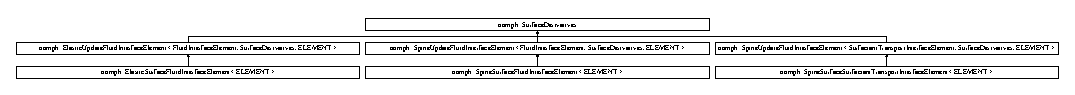
\includegraphics[height=0.834575cm]{classoomph_1_1SurfaceDerivatives}
\end{center}
\end{figure}
\subsection*{Public Member Functions}
\begin{DoxyCompactItemize}
\item 
\hyperlink{classoomph_1_1SurfaceDerivatives_a7bd520c805a4444073f5b05501d747fd}{Surface\+Derivatives} ()
\end{DoxyCompactItemize}
\subsection*{Protected Member Functions}
\begin{DoxyCompactItemize}
\item 
double \hyperlink{classoomph_1_1SurfaceDerivatives_a44e841bfa4ad82dcb87e672c821ffde7}{compute\+\_\+surface\+\_\+derivatives} (const \hyperlink{classoomph_1_1Shape}{Shape} \&psi, const \hyperlink{classoomph_1_1DShape}{D\+Shape} \&dpsids, const \hyperlink{classoomph_1_1DenseMatrix}{Dense\+Matrix}$<$ double $>$ \&interpolated\+\_\+t, const \hyperlink{classoomph_1_1Vector}{Vector}$<$ double $>$ \&interpolated\+\_\+x, \hyperlink{classoomph_1_1DShape}{D\+Shape} \&surface\+\_\+gradient, \hyperlink{classoomph_1_1DShape}{D\+Shape} \&surface\+\_\+divergence)
\begin{DoxyCompactList}\small\item\em Fill in the specific surface derivative calculations. \end{DoxyCompactList}\end{DoxyCompactItemize}


\subsection{Detailed Description}
Class that establishes the surface derivative functions for Surface\+Interface\+Elements (2D surfaces in 3D space) These are defined in a separate class so that they can be used by other interface equation-\/type classes. 

Definition at line 694 of file interface\+\_\+elements.\+h.



\subsection{Constructor \& Destructor Documentation}
\mbox{\Hypertarget{classoomph_1_1SurfaceDerivatives_a7bd520c805a4444073f5b05501d747fd}\label{classoomph_1_1SurfaceDerivatives_a7bd520c805a4444073f5b05501d747fd}} 
\index{oomph\+::\+Surface\+Derivatives@{oomph\+::\+Surface\+Derivatives}!Surface\+Derivatives@{Surface\+Derivatives}}
\index{Surface\+Derivatives@{Surface\+Derivatives}!oomph\+::\+Surface\+Derivatives@{oomph\+::\+Surface\+Derivatives}}
\subsubsection{\texorpdfstring{Surface\+Derivatives()}{SurfaceDerivatives()}}
{\footnotesize\ttfamily oomph\+::\+Surface\+Derivatives\+::\+Surface\+Derivatives (\begin{DoxyParamCaption}{ }\end{DoxyParamCaption})\hspace{0.3cm}{\ttfamily [inline]}}



Definition at line 698 of file interface\+\_\+elements.\+h.



References oomph\+::\+Face\+Element\+::interpolated\+\_\+x().



\subsection{Member Function Documentation}
\mbox{\Hypertarget{classoomph_1_1SurfaceDerivatives_a44e841bfa4ad82dcb87e672c821ffde7}\label{classoomph_1_1SurfaceDerivatives_a44e841bfa4ad82dcb87e672c821ffde7}} 
\index{oomph\+::\+Surface\+Derivatives@{oomph\+::\+Surface\+Derivatives}!compute\+\_\+surface\+\_\+derivatives@{compute\+\_\+surface\+\_\+derivatives}}
\index{compute\+\_\+surface\+\_\+derivatives@{compute\+\_\+surface\+\_\+derivatives}!oomph\+::\+Surface\+Derivatives@{oomph\+::\+Surface\+Derivatives}}
\subsubsection{\texorpdfstring{compute\+\_\+surface\+\_\+derivatives()}{compute\_surface\_derivatives()}}
{\footnotesize\ttfamily double oomph\+::\+Surface\+Derivatives\+::compute\+\_\+surface\+\_\+derivatives (\begin{DoxyParamCaption}\item[{const \hyperlink{classoomph_1_1Shape}{Shape} \&}]{psi,  }\item[{const \hyperlink{classoomph_1_1DShape}{D\+Shape} \&}]{dpsids,  }\item[{const \hyperlink{classoomph_1_1DenseMatrix}{Dense\+Matrix}$<$ double $>$ \&}]{interpolated\+\_\+t,  }\item[{const \hyperlink{classoomph_1_1Vector}{Vector}$<$ double $>$ \&}]{interpolated\+\_\+x,  }\item[{\hyperlink{classoomph_1_1DShape}{D\+Shape} \&}]{surface\+\_\+gradient,  }\item[{\hyperlink{classoomph_1_1DShape}{D\+Shape} \&}]{surface\+\_\+divergence }\end{DoxyParamCaption})\hspace{0.3cm}{\ttfamily [protected]}}



Fill in the specific surface derivative calculations. 

Specialise the surface derivatives for 2D surface case. 

Definition at line 851 of file interface\+\_\+elements.\+cc.



References i, and oomph\+::\+Shape\+::nindex1().



The documentation for this class was generated from the following files\+:\begin{DoxyCompactItemize}
\item 
\hyperlink{interface__elements_8h}{interface\+\_\+elements.\+h}\item 
\hyperlink{interface__elements_8cc}{interface\+\_\+elements.\+cc}\end{DoxyCompactItemize}

\hypertarget{classoomph_1_1SurfaceVolumeConstraintBoundingElement}{}\section{oomph\+:\+:Surface\+Volume\+Constraint\+Bounding\+Element Class Reference}
\label{classoomph_1_1SurfaceVolumeConstraintBoundingElement}\index{oomph\+::\+Surface\+Volume\+Constraint\+Bounding\+Element@{oomph\+::\+Surface\+Volume\+Constraint\+Bounding\+Element}}


{\ttfamily \#include $<$constrained\+\_\+volume\+\_\+elements.\+h$>$}

Inheritance diagram for oomph\+:\+:Surface\+Volume\+Constraint\+Bounding\+Element\+:\begin{figure}[H]
\begin{center}
\leavevmode
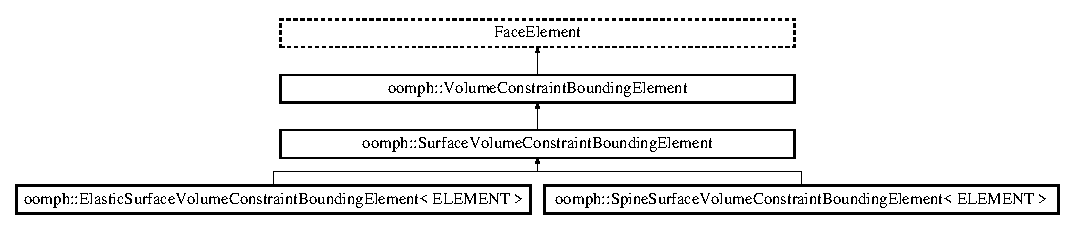
\includegraphics[height=2.647754cm]{classoomph_1_1SurfaceVolumeConstraintBoundingElement}
\end{center}
\end{figure}
\subsection*{Public Member Functions}
\begin{DoxyCompactItemize}
\item 
\hyperlink{classoomph_1_1SurfaceVolumeConstraintBoundingElement_a1dc9bb792bbce8f69f063a33934fc84e}{Surface\+Volume\+Constraint\+Bounding\+Element} ()
\begin{DoxyCompactList}\small\item\em Empty Contructor. \end{DoxyCompactList}\item 
\hyperlink{classoomph_1_1SurfaceVolumeConstraintBoundingElement_a9545195abf877c791208081022f30672}{$\sim$\+Surface\+Volume\+Constraint\+Bounding\+Element} ()
\begin{DoxyCompactList}\small\item\em Empty Desctructor. \end{DoxyCompactList}\end{DoxyCompactItemize}
\subsection*{Protected Member Functions}
\begin{DoxyCompactItemize}
\item 
void \hyperlink{classoomph_1_1SurfaceVolumeConstraintBoundingElement_a5813fa65063eb55a5b264539d77cac88}{fill\+\_\+in\+\_\+generic\+\_\+residual\+\_\+contribution\+\_\+volume\+\_\+constraint} (Vector$<$ double $>$ \&residuals)
\begin{DoxyCompactList}\small\item\em Helper function to fill in contributions to residuals (remember that part of the residual is added by the the associated \hyperlink{classoomph_1_1VolumeConstraintElement}{Volume\+Constraint\+Element}). This is specific for 2D surface elements that bound 3D cartesian fluid elements. \end{DoxyCompactList}\end{DoxyCompactItemize}
\subsection*{Additional Inherited Members}


\subsection{Detailed Description}
Two-\/dimensional interface elements that allow the application of a volume constraint on the region bounded by these elements. The volume is computed by integrating x.\+n around the boundary of the domain and then dividing by three. The sign is chosen so that the volume will be positive when the elements surround a fluid domain.

These elements must be used together with the associated \hyperlink{classoomph_1_1VolumeConstraintElement}{Volume\+Constraint\+Element}, which stores the value of the target volume. 

Definition at line 728 of file constrained\+\_\+volume\+\_\+elements.\+h.



\subsection{Constructor \& Destructor Documentation}
\mbox{\Hypertarget{classoomph_1_1SurfaceVolumeConstraintBoundingElement_a1dc9bb792bbce8f69f063a33934fc84e}\label{classoomph_1_1SurfaceVolumeConstraintBoundingElement_a1dc9bb792bbce8f69f063a33934fc84e}} 
\index{oomph\+::\+Surface\+Volume\+Constraint\+Bounding\+Element@{oomph\+::\+Surface\+Volume\+Constraint\+Bounding\+Element}!Surface\+Volume\+Constraint\+Bounding\+Element@{Surface\+Volume\+Constraint\+Bounding\+Element}}
\index{Surface\+Volume\+Constraint\+Bounding\+Element@{Surface\+Volume\+Constraint\+Bounding\+Element}!oomph\+::\+Surface\+Volume\+Constraint\+Bounding\+Element@{oomph\+::\+Surface\+Volume\+Constraint\+Bounding\+Element}}
\subsubsection{\texorpdfstring{Surface\+Volume\+Constraint\+Bounding\+Element()}{SurfaceVolumeConstraintBoundingElement()}}
{\footnotesize\ttfamily oomph\+::\+Surface\+Volume\+Constraint\+Bounding\+Element\+::\+Surface\+Volume\+Constraint\+Bounding\+Element (\begin{DoxyParamCaption}{ }\end{DoxyParamCaption})\hspace{0.3cm}{\ttfamily [inline]}}



Empty Contructor. 



Definition at line 744 of file constrained\+\_\+volume\+\_\+elements.\+h.

\mbox{\Hypertarget{classoomph_1_1SurfaceVolumeConstraintBoundingElement_a9545195abf877c791208081022f30672}\label{classoomph_1_1SurfaceVolumeConstraintBoundingElement_a9545195abf877c791208081022f30672}} 
\index{oomph\+::\+Surface\+Volume\+Constraint\+Bounding\+Element@{oomph\+::\+Surface\+Volume\+Constraint\+Bounding\+Element}!````~Surface\+Volume\+Constraint\+Bounding\+Element@{$\sim$\+Surface\+Volume\+Constraint\+Bounding\+Element}}
\index{````~Surface\+Volume\+Constraint\+Bounding\+Element@{$\sim$\+Surface\+Volume\+Constraint\+Bounding\+Element}!oomph\+::\+Surface\+Volume\+Constraint\+Bounding\+Element@{oomph\+::\+Surface\+Volume\+Constraint\+Bounding\+Element}}
\subsubsection{\texorpdfstring{$\sim$\+Surface\+Volume\+Constraint\+Bounding\+Element()}{~SurfaceVolumeConstraintBoundingElement()}}
{\footnotesize\ttfamily oomph\+::\+Surface\+Volume\+Constraint\+Bounding\+Element\+::$\sim$\+Surface\+Volume\+Constraint\+Bounding\+Element (\begin{DoxyParamCaption}{ }\end{DoxyParamCaption})\hspace{0.3cm}{\ttfamily [inline]}}



Empty Desctructor. 



Definition at line 748 of file constrained\+\_\+volume\+\_\+elements.\+h.



\subsection{Member Function Documentation}
\mbox{\Hypertarget{classoomph_1_1SurfaceVolumeConstraintBoundingElement_a5813fa65063eb55a5b264539d77cac88}\label{classoomph_1_1SurfaceVolumeConstraintBoundingElement_a5813fa65063eb55a5b264539d77cac88}} 
\index{oomph\+::\+Surface\+Volume\+Constraint\+Bounding\+Element@{oomph\+::\+Surface\+Volume\+Constraint\+Bounding\+Element}!fill\+\_\+in\+\_\+generic\+\_\+residual\+\_\+contribution\+\_\+volume\+\_\+constraint@{fill\+\_\+in\+\_\+generic\+\_\+residual\+\_\+contribution\+\_\+volume\+\_\+constraint}}
\index{fill\+\_\+in\+\_\+generic\+\_\+residual\+\_\+contribution\+\_\+volume\+\_\+constraint@{fill\+\_\+in\+\_\+generic\+\_\+residual\+\_\+contribution\+\_\+volume\+\_\+constraint}!oomph\+::\+Surface\+Volume\+Constraint\+Bounding\+Element@{oomph\+::\+Surface\+Volume\+Constraint\+Bounding\+Element}}
\subsubsection{\texorpdfstring{fill\+\_\+in\+\_\+generic\+\_\+residual\+\_\+contribution\+\_\+volume\+\_\+constraint()}{fill\_in\_generic\_residual\_contribution\_volume\_constraint()}}
{\footnotesize\ttfamily void oomph\+::\+Surface\+Volume\+Constraint\+Bounding\+Element\+::fill\+\_\+in\+\_\+generic\+\_\+residual\+\_\+contribution\+\_\+volume\+\_\+constraint (\begin{DoxyParamCaption}\item[{Vector$<$ double $>$ \&}]{residuals }\end{DoxyParamCaption})\hspace{0.3cm}{\ttfamily [protected]}, {\ttfamily [virtual]}}



Helper function to fill in contributions to residuals (remember that part of the residual is added by the the associated \hyperlink{classoomph_1_1VolumeConstraintElement}{Volume\+Constraint\+Element}). This is specific for 2D surface elements that bound 3D cartesian fluid elements. 



Implements \hyperlink{classoomph_1_1VolumeConstraintBoundingElement_a717f1085709bd8820b8043ff94ecb0c5}{oomph\+::\+Volume\+Constraint\+Bounding\+Element}.



Definition at line 442 of file constrained\+\_\+volume\+\_\+elements.\+cc.



References oomph\+::\+Volume\+Constraint\+Element\+::ptraded\+\_\+local\+\_\+eqn().



Referenced by oomph\+::\+Axisymmetric\+Volume\+Constraint\+Bounding\+Element\+::fill\+\_\+in\+\_\+generic\+\_\+residual\+\_\+contribution\+\_\+volume\+\_\+constraint().



The documentation for this class was generated from the following files\+:\begin{DoxyCompactItemize}
\item 
\hyperlink{constrained__volume__elements_8h}{constrained\+\_\+volume\+\_\+elements.\+h}\item 
\hyperlink{constrained__volume__elements_8cc}{constrained\+\_\+volume\+\_\+elements.\+cc}\end{DoxyCompactItemize}

\hypertarget{classoomph_1_1SurfactantTransportInterfaceElement}{}\section{oomph\+:\+:Surfactant\+Transport\+Interface\+Element Class Reference}
\label{classoomph_1_1SurfactantTransportInterfaceElement}\index{oomph\+::\+Surfactant\+Transport\+Interface\+Element@{oomph\+::\+Surfactant\+Transport\+Interface\+Element}}


{\ttfamily \#include $<$surfactant\+\_\+transport\+\_\+elements.\+h$>$}

Inheritance diagram for oomph\+:\+:Surfactant\+Transport\+Interface\+Element\+:\begin{figure}[H]
\begin{center}
\leavevmode
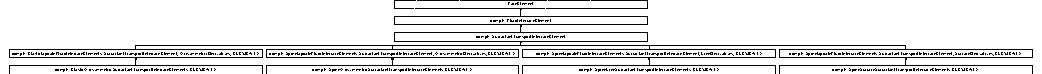
\includegraphics[height=0.992908cm]{classoomph_1_1SurfactantTransportInterfaceElement}
\end{center}
\end{figure}
\subsection*{Public Member Functions}
\begin{DoxyCompactItemize}
\item 
\hyperlink{classoomph_1_1SurfactantTransportInterfaceElement_a8934ab8e723427ed39298c592b2876a5}{Surfactant\+Transport\+Interface\+Element} ()
\item 
void \hyperlink{classoomph_1_1SurfactantTransportInterfaceElement_aaf7988dfac3e02018c591f2f9e34f644}{set\+\_\+c\+\_\+index} (const Vector$<$ unsigned $>$ \&c\+\_\+index)
\item 
double \hyperlink{classoomph_1_1SurfactantTransportInterfaceElement_a79003d87401ad6106b8d10373ff12e73}{beta} ()
\begin{DoxyCompactList}\small\item\em Return the Elasticity number. \end{DoxyCompactList}\item 
double \hyperlink{classoomph_1_1SurfactantTransportInterfaceElement_ac945c28401b92a061e3e245e83541c55}{peclet\+\_\+s} ()
\begin{DoxyCompactList}\small\item\em Return the surface peclect number. \end{DoxyCompactList}\item 
double \hyperlink{classoomph_1_1SurfactantTransportInterfaceElement_acb4ff16ed90e79ffe9e4156ef030d689}{peclet\+\_\+strouhal\+\_\+s} ()
\begin{DoxyCompactList}\small\item\em Return the surface peclect strouhal number. \end{DoxyCompactList}\item 
double $\ast$\& \hyperlink{classoomph_1_1SurfactantTransportInterfaceElement_a7f64f64c3b5ad3abe6e09bb10a039298}{beta\+\_\+pt} ()
\begin{DoxyCompactList}\small\item\em Access function for pointer to the Elasticity number. \end{DoxyCompactList}\item 
double $\ast$\& \hyperlink{classoomph_1_1SurfactantTransportInterfaceElement_a3ce30a3705a18034585c80d2f9757099}{peclet\+\_\+s\+\_\+pt} ()
\begin{DoxyCompactList}\small\item\em Access function for pointer to the surface Peclet number. \end{DoxyCompactList}\item 
double $\ast$\& \hyperlink{classoomph_1_1SurfactantTransportInterfaceElement_a422fa3f65ca6635b6bfbe993e01bce72}{peclet\+\_\+strouhal\+\_\+s\+\_\+pt} ()
\begin{DoxyCompactList}\small\item\em Access function for pointer to the surface Peclet x Strouhal number. \end{DoxyCompactList}\item 
void \hyperlink{classoomph_1_1SurfactantTransportInterfaceElement_a280f065d9cb85438c0fe4f7cd95d14b3}{output} (std\+::ostream \&outfile)
\begin{DoxyCompactList}\small\item\em Overload the output function. \end{DoxyCompactList}\item 
void \hyperlink{classoomph_1_1SurfactantTransportInterfaceElement_aebc3ed4954b636f4992a212c7973c670}{output} (std\+::ostream \&outfile, const unsigned \&n\+\_\+plot)
\begin{DoxyCompactList}\small\item\em Overload the output function. \end{DoxyCompactList}\item 
void \hyperlink{classoomph_1_1SurfactantTransportInterfaceElement_a32ae151a017b122dd7a4c03511afbcc9}{output} (F\+I\+LE $\ast$file\+\_\+pt)
\begin{DoxyCompactList}\small\item\em Overload the C-\/style output function. \end{DoxyCompactList}\item 
void \hyperlink{classoomph_1_1SurfactantTransportInterfaceElement_ad41354dbe1ae8291e3330b3752b525f8}{output} (F\+I\+LE $\ast$file\+\_\+pt, const unsigned \&n\+\_\+plot)
\begin{DoxyCompactList}\small\item\em C-\/style Output function. \end{DoxyCompactList}\item 
double \hyperlink{classoomph_1_1SurfactantTransportInterfaceElement_a703c35a6da2925926c976957f2da77c4}{integrate\+\_\+c} ()
\begin{DoxyCompactList}\small\item\em Compute the concentration intergated over the surface area. \end{DoxyCompactList}\end{DoxyCompactItemize}
\subsection*{Protected Member Functions}
\begin{DoxyCompactItemize}
\item 
double \hyperlink{classoomph_1_1SurfactantTransportInterfaceElement_a9da12df06b20e5f1ce0736acfc7e8d83}{interpolated\+\_\+C} (const Vector$<$ double $>$ \&s)
\begin{DoxyCompactList}\small\item\em Get the surfactant concentration. \end{DoxyCompactList}\item 
double \hyperlink{classoomph_1_1SurfactantTransportInterfaceElement_a7b5cc851b94d836a3caa2130cbf45bec}{dcdt\+\_\+surface} (const unsigned \&l) const
\begin{DoxyCompactList}\small\item\em The time derivative of the surface concentration. \end{DoxyCompactList}\item 
double \hyperlink{classoomph_1_1SurfactantTransportInterfaceElement_a1710057c610ccccc06ef41f34f086aae}{sigma} (const Vector$<$ double $>$ \&s)
\item 
double \hyperlink{classoomph_1_1SurfactantTransportInterfaceElement_ad39e6040101db7d9338928b3c2343623}{dsigma\+\_\+dC} (const Vector$<$ double $>$ \&s)
\item 
void \hyperlink{classoomph_1_1SurfactantTransportInterfaceElement_adedf33390efdf652e169f8bd38eb2350}{add\+\_\+additional\+\_\+residual\+\_\+contributions\+\_\+interface} (Vector$<$ double $>$ \&residuals, Dense\+Matrix$<$ double $>$ \&jacobian, const unsigned \&flag, const Shape \&psif, const D\+Shape \&dpsifds, const D\+Shape \&dpsifdS, const D\+Shape \&dpsifd\+S\+\_\+div, const Vector$<$ double $>$ \&s, const Vector$<$ double $>$ \&interpolated\+\_\+x, const Vector$<$ double $>$ \&interpolated\+\_\+n, const double \&W, const double \&J)
\begin{DoxyCompactList}\small\item\em Overload the Helper function to calculate the residuals and jacobian entries. This particular function ensures that the additional entries are calculated inside the integration loop. \end{DoxyCompactList}\item 
void \hyperlink{classoomph_1_1SurfactantTransportInterfaceElement_a7c0f9b63cea887a4a65abbe9aeb3b3cf}{fill\+\_\+in\+\_\+contribution\+\_\+to\+\_\+jacobian\+\_\+and\+\_\+mass\+\_\+matrix} (Vector$<$ double $>$ \&residuals, Dense\+Matrix$<$ double $>$ \&jacobian, Dense\+Matrix$<$ double $>$ \&mass\+\_\+matrix)
\end{DoxyCompactItemize}
\subsection*{Protected Attributes}
\begin{DoxyCompactItemize}
\item 
Vector$<$ unsigned $>$ \hyperlink{classoomph_1_1SurfactantTransportInterfaceElement_a26727fb7b57f88d3e1bdf4f2dd9f3b02}{C\+\_\+index}
\end{DoxyCompactItemize}
\subsection*{Static Protected Attributes}
\begin{DoxyCompactItemize}
\item 
static double \hyperlink{classoomph_1_1SurfactantTransportInterfaceElement_ae2c6f40fd7bc427636ac25c23d816e74}{Default\+\_\+\+Physical\+\_\+\+Constant\+\_\+\+Value} = 1.\+0
\begin{DoxyCompactList}\small\item\em Default value of the physical constants. \end{DoxyCompactList}\end{DoxyCompactItemize}
\subsection*{Private Attributes}
\begin{DoxyCompactItemize}
\item 
double $\ast$ \hyperlink{classoomph_1_1SurfactantTransportInterfaceElement_ab5140eb5a576820321032b10a894b530}{Beta\+\_\+pt}
\begin{DoxyCompactList}\small\item\em Pointer to an Elasticity number. \end{DoxyCompactList}\item 
double $\ast$ \hyperlink{classoomph_1_1SurfactantTransportInterfaceElement_a50b4771707337535c081324f2f0d8c30}{Peclet\+\_\+\+S\+\_\+pt}
\begin{DoxyCompactList}\small\item\em Pointer to Surface Peclet number. \end{DoxyCompactList}\item 
double $\ast$ \hyperlink{classoomph_1_1SurfactantTransportInterfaceElement_a3c4a6abcb3795ee53baff49864cd0020}{Peclet\+\_\+\+Strouhal\+\_\+\+S\+\_\+pt}
\begin{DoxyCompactList}\small\item\em Pointer to the surface Peclect Strouhal number. \end{DoxyCompactList}\end{DoxyCompactItemize}


\subsection{Detailed Description}
Generic surfactant transport equations implemented independently of the dimension and then specialised using the generic mechanisms introduce in the Fluid\+Interface\+Elements 

Definition at line 53 of file surfactant\+\_\+transport\+\_\+elements.\+h.



\subsection{Constructor \& Destructor Documentation}
\mbox{\Hypertarget{classoomph_1_1SurfactantTransportInterfaceElement_a8934ab8e723427ed39298c592b2876a5}\label{classoomph_1_1SurfactantTransportInterfaceElement_a8934ab8e723427ed39298c592b2876a5}} 
\index{oomph\+::\+Surfactant\+Transport\+Interface\+Element@{oomph\+::\+Surfactant\+Transport\+Interface\+Element}!Surfactant\+Transport\+Interface\+Element@{Surfactant\+Transport\+Interface\+Element}}
\index{Surfactant\+Transport\+Interface\+Element@{Surfactant\+Transport\+Interface\+Element}!oomph\+::\+Surfactant\+Transport\+Interface\+Element@{oomph\+::\+Surfactant\+Transport\+Interface\+Element}}
\subsubsection{\texorpdfstring{Surfactant\+Transport\+Interface\+Element()}{SurfactantTransportInterfaceElement()}}
{\footnotesize\ttfamily oomph\+::\+Surfactant\+Transport\+Interface\+Element\+::\+Surfactant\+Transport\+Interface\+Element (\begin{DoxyParamCaption}{ }\end{DoxyParamCaption})\hspace{0.3cm}{\ttfamily [inline]}}

Constructor that passes the bulk element and face index down to the underlying 

Definition at line 119 of file surfactant\+\_\+transport\+\_\+elements.\+h.



References Default\+\_\+\+Physical\+\_\+\+Constant\+\_\+\+Value.



\subsection{Member Function Documentation}
\mbox{\Hypertarget{classoomph_1_1SurfactantTransportInterfaceElement_adedf33390efdf652e169f8bd38eb2350}\label{classoomph_1_1SurfactantTransportInterfaceElement_adedf33390efdf652e169f8bd38eb2350}} 
\index{oomph\+::\+Surfactant\+Transport\+Interface\+Element@{oomph\+::\+Surfactant\+Transport\+Interface\+Element}!add\+\_\+additional\+\_\+residual\+\_\+contributions\+\_\+interface@{add\+\_\+additional\+\_\+residual\+\_\+contributions\+\_\+interface}}
\index{add\+\_\+additional\+\_\+residual\+\_\+contributions\+\_\+interface@{add\+\_\+additional\+\_\+residual\+\_\+contributions\+\_\+interface}!oomph\+::\+Surfactant\+Transport\+Interface\+Element@{oomph\+::\+Surfactant\+Transport\+Interface\+Element}}
\subsubsection{\texorpdfstring{add\+\_\+additional\+\_\+residual\+\_\+contributions\+\_\+interface()}{add\_additional\_residual\_contributions\_interface()}}
{\footnotesize\ttfamily void oomph\+::\+Surfactant\+Transport\+Interface\+Element\+::add\+\_\+additional\+\_\+residual\+\_\+contributions\+\_\+interface (\begin{DoxyParamCaption}\item[{Vector$<$ double $>$ \&}]{residuals,  }\item[{Dense\+Matrix$<$ double $>$ \&}]{jacobian,  }\item[{const unsigned \&}]{flag,  }\item[{const Shape \&}]{psif,  }\item[{const D\+Shape \&}]{dpsifds,  }\item[{const D\+Shape \&}]{dpsifdS,  }\item[{const D\+Shape \&}]{dpsifd\+S\+\_\+div,  }\item[{const Vector$<$ double $>$ \&}]{s,  }\item[{const Vector$<$ double $>$ \&}]{interpolated\+\_\+x,  }\item[{const Vector$<$ double $>$ \&}]{interpolated\+\_\+n,  }\item[{const double \&}]{W,  }\item[{const double \&}]{J }\end{DoxyParamCaption})\hspace{0.3cm}{\ttfamily [protected]}, {\ttfamily [virtual]}}



Overload the Helper function to calculate the residuals and jacobian entries. This particular function ensures that the additional entries are calculated inside the integration loop. 



Reimplemented from \hyperlink{classoomph_1_1FluidInterfaceElement_a0bc278bb201b861f47dc846453be4c06}{oomph\+::\+Fluid\+Interface\+Element}.



Reimplemented in \hyperlink{classoomph_1_1ElasticUpdateFluidInterfaceElement_a15c3d2912325ace17676366c1469121f}{oomph\+::\+Elastic\+Update\+Fluid\+Interface\+Element$<$ Surfactant\+Transport\+Interface\+Element, Axisymmetric\+Derivatives, E\+L\+E\+M\+E\+N\+T $>$}, \hyperlink{classoomph_1_1SpineUpdateFluidInterfaceElement_a3958845051cafecd8e73745fc04c7a78}{oomph\+::\+Spine\+Update\+Fluid\+Interface\+Element$<$ Surfactant\+Transport\+Interface\+Element, Line\+Derivatives, E\+L\+E\+M\+E\+N\+T $>$}, \hyperlink{classoomph_1_1SpineUpdateFluidInterfaceElement_a3958845051cafecd8e73745fc04c7a78}{oomph\+::\+Spine\+Update\+Fluid\+Interface\+Element$<$ Surfactant\+Transport\+Interface\+Element, Axisymmetric\+Derivatives, E\+L\+E\+M\+E\+N\+T $>$}, and \hyperlink{classoomph_1_1SpineUpdateFluidInterfaceElement_a3958845051cafecd8e73745fc04c7a78}{oomph\+::\+Spine\+Update\+Fluid\+Interface\+Element$<$ Surfactant\+Transport\+Interface\+Element, Surface\+Derivatives, E\+L\+E\+M\+E\+N\+T $>$}.



Definition at line 122 of file surfactant\+\_\+transport\+\_\+elements.\+cc.



References C\+\_\+index, oomph\+::\+Fluid\+Interface\+Element\+::ca(), dcdt\+\_\+surface(), dsigma\+\_\+d\+C(), interpolated\+\_\+\+C(), oomph\+::\+Fluid\+Interface\+Element\+::interpolated\+\_\+u(), peclet\+\_\+s(), and oomph\+::\+Fluid\+Interface\+Element\+::\+U\+\_\+index\+\_\+interface.



Referenced by dsigma\+\_\+d\+C().

\mbox{\Hypertarget{classoomph_1_1SurfactantTransportInterfaceElement_a79003d87401ad6106b8d10373ff12e73}\label{classoomph_1_1SurfactantTransportInterfaceElement_a79003d87401ad6106b8d10373ff12e73}} 
\index{oomph\+::\+Surfactant\+Transport\+Interface\+Element@{oomph\+::\+Surfactant\+Transport\+Interface\+Element}!beta@{beta}}
\index{beta@{beta}!oomph\+::\+Surfactant\+Transport\+Interface\+Element@{oomph\+::\+Surfactant\+Transport\+Interface\+Element}}
\subsubsection{\texorpdfstring{beta()}{beta()}}
{\footnotesize\ttfamily double oomph\+::\+Surfactant\+Transport\+Interface\+Element\+::beta (\begin{DoxyParamCaption}{ }\end{DoxyParamCaption})\hspace{0.3cm}{\ttfamily [inline]}}



Return the Elasticity number. 



Definition at line 131 of file surfactant\+\_\+transport\+\_\+elements.\+h.



References Beta\+\_\+pt.



Referenced by dsigma\+\_\+d\+C(), and sigma().

\mbox{\Hypertarget{classoomph_1_1SurfactantTransportInterfaceElement_a7f64f64c3b5ad3abe6e09bb10a039298}\label{classoomph_1_1SurfactantTransportInterfaceElement_a7f64f64c3b5ad3abe6e09bb10a039298}} 
\index{oomph\+::\+Surfactant\+Transport\+Interface\+Element@{oomph\+::\+Surfactant\+Transport\+Interface\+Element}!beta\+\_\+pt@{beta\+\_\+pt}}
\index{beta\+\_\+pt@{beta\+\_\+pt}!oomph\+::\+Surfactant\+Transport\+Interface\+Element@{oomph\+::\+Surfactant\+Transport\+Interface\+Element}}
\subsubsection{\texorpdfstring{beta\+\_\+pt()}{beta\_pt()}}
{\footnotesize\ttfamily double$\ast$ \& oomph\+::\+Surfactant\+Transport\+Interface\+Element\+::beta\+\_\+pt (\begin{DoxyParamCaption}{ }\end{DoxyParamCaption})\hspace{0.3cm}{\ttfamily [inline]}}



Access function for pointer to the Elasticity number. 



Definition at line 140 of file surfactant\+\_\+transport\+\_\+elements.\+h.



References Beta\+\_\+pt.

\mbox{\Hypertarget{classoomph_1_1SurfactantTransportInterfaceElement_a7b5cc851b94d836a3caa2130cbf45bec}\label{classoomph_1_1SurfactantTransportInterfaceElement_a7b5cc851b94d836a3caa2130cbf45bec}} 
\index{oomph\+::\+Surfactant\+Transport\+Interface\+Element@{oomph\+::\+Surfactant\+Transport\+Interface\+Element}!dcdt\+\_\+surface@{dcdt\+\_\+surface}}
\index{dcdt\+\_\+surface@{dcdt\+\_\+surface}!oomph\+::\+Surfactant\+Transport\+Interface\+Element@{oomph\+::\+Surfactant\+Transport\+Interface\+Element}}
\subsubsection{\texorpdfstring{dcdt\+\_\+surface()}{dcdt\_surface()}}
{\footnotesize\ttfamily double oomph\+::\+Surfactant\+Transport\+Interface\+Element\+::dcdt\+\_\+surface (\begin{DoxyParamCaption}\item[{const unsigned \&}]{l }\end{DoxyParamCaption}) const\hspace{0.3cm}{\ttfamily [protected]}}



The time derivative of the surface concentration. 



Definition at line 71 of file surfactant\+\_\+transport\+\_\+elements.\+cc.



References C\+\_\+index.



Referenced by add\+\_\+additional\+\_\+residual\+\_\+contributions\+\_\+interface().

\mbox{\Hypertarget{classoomph_1_1SurfactantTransportInterfaceElement_ad39e6040101db7d9338928b3c2343623}\label{classoomph_1_1SurfactantTransportInterfaceElement_ad39e6040101db7d9338928b3c2343623}} 
\index{oomph\+::\+Surfactant\+Transport\+Interface\+Element@{oomph\+::\+Surfactant\+Transport\+Interface\+Element}!dsigma\+\_\+dC@{dsigma\+\_\+dC}}
\index{dsigma\+\_\+dC@{dsigma\+\_\+dC}!oomph\+::\+Surfactant\+Transport\+Interface\+Element@{oomph\+::\+Surfactant\+Transport\+Interface\+Element}}
\subsubsection{\texorpdfstring{dsigma\+\_\+d\+C()}{dsigma\_dC()}}
{\footnotesize\ttfamily double oomph\+::\+Surfactant\+Transport\+Interface\+Element\+::dsigma\+\_\+dC (\begin{DoxyParamCaption}\item[{const Vector$<$ double $>$ \&}]{s }\end{DoxyParamCaption})\hspace{0.3cm}{\ttfamily [inline]}, {\ttfamily [protected]}}

Return the derivative of sigma with respect to C For use in computing the Jacobian 

Definition at line 89 of file surfactant\+\_\+transport\+\_\+elements.\+h.



References add\+\_\+additional\+\_\+residual\+\_\+contributions\+\_\+interface(), and beta().



Referenced by add\+\_\+additional\+\_\+residual\+\_\+contributions\+\_\+interface().

\mbox{\Hypertarget{classoomph_1_1SurfactantTransportInterfaceElement_a7c0f9b63cea887a4a65abbe9aeb3b3cf}\label{classoomph_1_1SurfactantTransportInterfaceElement_a7c0f9b63cea887a4a65abbe9aeb3b3cf}} 
\index{oomph\+::\+Surfactant\+Transport\+Interface\+Element@{oomph\+::\+Surfactant\+Transport\+Interface\+Element}!fill\+\_\+in\+\_\+contribution\+\_\+to\+\_\+jacobian\+\_\+and\+\_\+mass\+\_\+matrix@{fill\+\_\+in\+\_\+contribution\+\_\+to\+\_\+jacobian\+\_\+and\+\_\+mass\+\_\+matrix}}
\index{fill\+\_\+in\+\_\+contribution\+\_\+to\+\_\+jacobian\+\_\+and\+\_\+mass\+\_\+matrix@{fill\+\_\+in\+\_\+contribution\+\_\+to\+\_\+jacobian\+\_\+and\+\_\+mass\+\_\+matrix}!oomph\+::\+Surfactant\+Transport\+Interface\+Element@{oomph\+::\+Surfactant\+Transport\+Interface\+Element}}
\subsubsection{\texorpdfstring{fill\+\_\+in\+\_\+contribution\+\_\+to\+\_\+jacobian\+\_\+and\+\_\+mass\+\_\+matrix()}{fill\_in\_contribution\_to\_jacobian\_and\_mass\_matrix()}}
{\footnotesize\ttfamily void oomph\+::\+Surfactant\+Transport\+Interface\+Element\+::fill\+\_\+in\+\_\+contribution\+\_\+to\+\_\+jacobian\+\_\+and\+\_\+mass\+\_\+matrix (\begin{DoxyParamCaption}\item[{Vector$<$ double $>$ \&}]{residuals,  }\item[{Dense\+Matrix$<$ double $>$ \&}]{jacobian,  }\item[{Dense\+Matrix$<$ double $>$ \&}]{mass\+\_\+matrix }\end{DoxyParamCaption})\hspace{0.3cm}{\ttfamily [inline]}, {\ttfamily [protected]}}

Add the element\textquotesingle{}s contribution to its residuals vector, jacobian matrix and mass matrix 

Definition at line 106 of file surfactant\+\_\+transport\+\_\+elements.\+h.

\mbox{\Hypertarget{classoomph_1_1SurfactantTransportInterfaceElement_a703c35a6da2925926c976957f2da77c4}\label{classoomph_1_1SurfactantTransportInterfaceElement_a703c35a6da2925926c976957f2da77c4}} 
\index{oomph\+::\+Surfactant\+Transport\+Interface\+Element@{oomph\+::\+Surfactant\+Transport\+Interface\+Element}!integrate\+\_\+c@{integrate\+\_\+c}}
\index{integrate\+\_\+c@{integrate\+\_\+c}!oomph\+::\+Surfactant\+Transport\+Interface\+Element@{oomph\+::\+Surfactant\+Transport\+Interface\+Element}}
\subsubsection{\texorpdfstring{integrate\+\_\+c()}{integrate\_c()}}
{\footnotesize\ttfamily double oomph\+::\+Surfactant\+Transport\+Interface\+Element\+::integrate\+\_\+c (\begin{DoxyParamCaption}{ }\end{DoxyParamCaption})}



Compute the concentration intergated over the surface area. 



Definition at line 347 of file surfactant\+\_\+transport\+\_\+elements.\+cc.



References C\+\_\+index, and oomph\+::\+Fluid\+Interface\+Element\+::compute\+\_\+surface\+\_\+derivatives().



Referenced by output().

\mbox{\Hypertarget{classoomph_1_1SurfactantTransportInterfaceElement_a9da12df06b20e5f1ce0736acfc7e8d83}\label{classoomph_1_1SurfactantTransportInterfaceElement_a9da12df06b20e5f1ce0736acfc7e8d83}} 
\index{oomph\+::\+Surfactant\+Transport\+Interface\+Element@{oomph\+::\+Surfactant\+Transport\+Interface\+Element}!interpolated\+\_\+C@{interpolated\+\_\+C}}
\index{interpolated\+\_\+C@{interpolated\+\_\+C}!oomph\+::\+Surfactant\+Transport\+Interface\+Element@{oomph\+::\+Surfactant\+Transport\+Interface\+Element}}
\subsubsection{\texorpdfstring{interpolated\+\_\+\+C()}{interpolated\_C()}}
{\footnotesize\ttfamily double oomph\+::\+Surfactant\+Transport\+Interface\+Element\+::interpolated\+\_\+C (\begin{DoxyParamCaption}\item[{const Vector$<$ double $>$ \&}]{s }\end{DoxyParamCaption})\hspace{0.3cm}{\ttfamily [protected]}}



Get the surfactant concentration. 



Definition at line 45 of file surfactant\+\_\+transport\+\_\+elements.\+cc.



References C\+\_\+index.



Referenced by add\+\_\+additional\+\_\+residual\+\_\+contributions\+\_\+interface(), and output().

\mbox{\Hypertarget{classoomph_1_1SurfactantTransportInterfaceElement_a280f065d9cb85438c0fe4f7cd95d14b3}\label{classoomph_1_1SurfactantTransportInterfaceElement_a280f065d9cb85438c0fe4f7cd95d14b3}} 
\index{oomph\+::\+Surfactant\+Transport\+Interface\+Element@{oomph\+::\+Surfactant\+Transport\+Interface\+Element}!output@{output}}
\index{output@{output}!oomph\+::\+Surfactant\+Transport\+Interface\+Element@{oomph\+::\+Surfactant\+Transport\+Interface\+Element}}
\subsubsection{\texorpdfstring{output()}{output()}\hspace{0.1cm}{\footnotesize\ttfamily [1/4]}}
{\footnotesize\ttfamily void oomph\+::\+Surfactant\+Transport\+Interface\+Element\+::output (\begin{DoxyParamCaption}\item[{std\+::ostream \&}]{outfile }\end{DoxyParamCaption})\hspace{0.3cm}{\ttfamily [inline]}}



Overload the output function. 



Definition at line 150 of file surfactant\+\_\+transport\+\_\+elements.\+h.

\mbox{\Hypertarget{classoomph_1_1SurfactantTransportInterfaceElement_aebc3ed4954b636f4992a212c7973c670}\label{classoomph_1_1SurfactantTransportInterfaceElement_aebc3ed4954b636f4992a212c7973c670}} 
\index{oomph\+::\+Surfactant\+Transport\+Interface\+Element@{oomph\+::\+Surfactant\+Transport\+Interface\+Element}!output@{output}}
\index{output@{output}!oomph\+::\+Surfactant\+Transport\+Interface\+Element@{oomph\+::\+Surfactant\+Transport\+Interface\+Element}}
\subsubsection{\texorpdfstring{output()}{output()}\hspace{0.1cm}{\footnotesize\ttfamily [2/4]}}
{\footnotesize\ttfamily void oomph\+::\+Surfactant\+Transport\+Interface\+Element\+::output (\begin{DoxyParamCaption}\item[{std\+::ostream \&}]{outfile,  }\item[{const unsigned \&}]{n\+\_\+plot }\end{DoxyParamCaption})}



Overload the output function. 



Definition at line 290 of file surfactant\+\_\+transport\+\_\+elements.\+cc.



References interpolated\+\_\+\+C(), oomph\+::\+Fluid\+Interface\+Element\+::interpolated\+\_\+u(), sigma(), oomph\+::\+Fluid\+Interface\+Element\+::u(), and oomph\+::\+Fluid\+Interface\+Element\+::\+U\+\_\+index\+\_\+interface.

\mbox{\Hypertarget{classoomph_1_1SurfactantTransportInterfaceElement_a32ae151a017b122dd7a4c03511afbcc9}\label{classoomph_1_1SurfactantTransportInterfaceElement_a32ae151a017b122dd7a4c03511afbcc9}} 
\index{oomph\+::\+Surfactant\+Transport\+Interface\+Element@{oomph\+::\+Surfactant\+Transport\+Interface\+Element}!output@{output}}
\index{output@{output}!oomph\+::\+Surfactant\+Transport\+Interface\+Element@{oomph\+::\+Surfactant\+Transport\+Interface\+Element}}
\subsubsection{\texorpdfstring{output()}{output()}\hspace{0.1cm}{\footnotesize\ttfamily [3/4]}}
{\footnotesize\ttfamily void oomph\+::\+Surfactant\+Transport\+Interface\+Element\+::output (\begin{DoxyParamCaption}\item[{F\+I\+LE $\ast$}]{file\+\_\+pt }\end{DoxyParamCaption})\hspace{0.3cm}{\ttfamily [inline]}}



Overload the C-\/style output function. 



Definition at line 155 of file surfactant\+\_\+transport\+\_\+elements.\+h.

\mbox{\Hypertarget{classoomph_1_1SurfactantTransportInterfaceElement_ad41354dbe1ae8291e3330b3752b525f8}\label{classoomph_1_1SurfactantTransportInterfaceElement_ad41354dbe1ae8291e3330b3752b525f8}} 
\index{oomph\+::\+Surfactant\+Transport\+Interface\+Element@{oomph\+::\+Surfactant\+Transport\+Interface\+Element}!output@{output}}
\index{output@{output}!oomph\+::\+Surfactant\+Transport\+Interface\+Element@{oomph\+::\+Surfactant\+Transport\+Interface\+Element}}
\subsubsection{\texorpdfstring{output()}{output()}\hspace{0.1cm}{\footnotesize\ttfamily [4/4]}}
{\footnotesize\ttfamily void oomph\+::\+Surfactant\+Transport\+Interface\+Element\+::output (\begin{DoxyParamCaption}\item[{F\+I\+LE $\ast$}]{file\+\_\+pt,  }\item[{const unsigned \&}]{n\+\_\+plot }\end{DoxyParamCaption})\hspace{0.3cm}{\ttfamily [inline]}}



C-\/style Output function. 



Definition at line 158 of file surfactant\+\_\+transport\+\_\+elements.\+h.



References integrate\+\_\+c().

\mbox{\Hypertarget{classoomph_1_1SurfactantTransportInterfaceElement_ac945c28401b92a061e3e245e83541c55}\label{classoomph_1_1SurfactantTransportInterfaceElement_ac945c28401b92a061e3e245e83541c55}} 
\index{oomph\+::\+Surfactant\+Transport\+Interface\+Element@{oomph\+::\+Surfactant\+Transport\+Interface\+Element}!peclet\+\_\+s@{peclet\+\_\+s}}
\index{peclet\+\_\+s@{peclet\+\_\+s}!oomph\+::\+Surfactant\+Transport\+Interface\+Element@{oomph\+::\+Surfactant\+Transport\+Interface\+Element}}
\subsubsection{\texorpdfstring{peclet\+\_\+s()}{peclet\_s()}}
{\footnotesize\ttfamily double oomph\+::\+Surfactant\+Transport\+Interface\+Element\+::peclet\+\_\+s (\begin{DoxyParamCaption}{ }\end{DoxyParamCaption})\hspace{0.3cm}{\ttfamily [inline]}}



Return the surface peclect number. 



Definition at line 134 of file surfactant\+\_\+transport\+\_\+elements.\+h.



References Peclet\+\_\+\+S\+\_\+pt.



Referenced by add\+\_\+additional\+\_\+residual\+\_\+contributions\+\_\+interface().

\mbox{\Hypertarget{classoomph_1_1SurfactantTransportInterfaceElement_a3ce30a3705a18034585c80d2f9757099}\label{classoomph_1_1SurfactantTransportInterfaceElement_a3ce30a3705a18034585c80d2f9757099}} 
\index{oomph\+::\+Surfactant\+Transport\+Interface\+Element@{oomph\+::\+Surfactant\+Transport\+Interface\+Element}!peclet\+\_\+s\+\_\+pt@{peclet\+\_\+s\+\_\+pt}}
\index{peclet\+\_\+s\+\_\+pt@{peclet\+\_\+s\+\_\+pt}!oomph\+::\+Surfactant\+Transport\+Interface\+Element@{oomph\+::\+Surfactant\+Transport\+Interface\+Element}}
\subsubsection{\texorpdfstring{peclet\+\_\+s\+\_\+pt()}{peclet\_s\_pt()}}
{\footnotesize\ttfamily double$\ast$ \& oomph\+::\+Surfactant\+Transport\+Interface\+Element\+::peclet\+\_\+s\+\_\+pt (\begin{DoxyParamCaption}{ }\end{DoxyParamCaption})\hspace{0.3cm}{\ttfamily [inline]}}



Access function for pointer to the surface Peclet number. 



Definition at line 143 of file surfactant\+\_\+transport\+\_\+elements.\+h.



References Peclet\+\_\+\+S\+\_\+pt.

\mbox{\Hypertarget{classoomph_1_1SurfactantTransportInterfaceElement_acb4ff16ed90e79ffe9e4156ef030d689}\label{classoomph_1_1SurfactantTransportInterfaceElement_acb4ff16ed90e79ffe9e4156ef030d689}} 
\index{oomph\+::\+Surfactant\+Transport\+Interface\+Element@{oomph\+::\+Surfactant\+Transport\+Interface\+Element}!peclet\+\_\+strouhal\+\_\+s@{peclet\+\_\+strouhal\+\_\+s}}
\index{peclet\+\_\+strouhal\+\_\+s@{peclet\+\_\+strouhal\+\_\+s}!oomph\+::\+Surfactant\+Transport\+Interface\+Element@{oomph\+::\+Surfactant\+Transport\+Interface\+Element}}
\subsubsection{\texorpdfstring{peclet\+\_\+strouhal\+\_\+s()}{peclet\_strouhal\_s()}}
{\footnotesize\ttfamily double oomph\+::\+Surfactant\+Transport\+Interface\+Element\+::peclet\+\_\+strouhal\+\_\+s (\begin{DoxyParamCaption}{ }\end{DoxyParamCaption})\hspace{0.3cm}{\ttfamily [inline]}}



Return the surface peclect strouhal number. 



Definition at line 137 of file surfactant\+\_\+transport\+\_\+elements.\+h.



References Peclet\+\_\+\+Strouhal\+\_\+\+S\+\_\+pt.

\mbox{\Hypertarget{classoomph_1_1SurfactantTransportInterfaceElement_a422fa3f65ca6635b6bfbe993e01bce72}\label{classoomph_1_1SurfactantTransportInterfaceElement_a422fa3f65ca6635b6bfbe993e01bce72}} 
\index{oomph\+::\+Surfactant\+Transport\+Interface\+Element@{oomph\+::\+Surfactant\+Transport\+Interface\+Element}!peclet\+\_\+strouhal\+\_\+s\+\_\+pt@{peclet\+\_\+strouhal\+\_\+s\+\_\+pt}}
\index{peclet\+\_\+strouhal\+\_\+s\+\_\+pt@{peclet\+\_\+strouhal\+\_\+s\+\_\+pt}!oomph\+::\+Surfactant\+Transport\+Interface\+Element@{oomph\+::\+Surfactant\+Transport\+Interface\+Element}}
\subsubsection{\texorpdfstring{peclet\+\_\+strouhal\+\_\+s\+\_\+pt()}{peclet\_strouhal\_s\_pt()}}
{\footnotesize\ttfamily double$\ast$ \& oomph\+::\+Surfactant\+Transport\+Interface\+Element\+::peclet\+\_\+strouhal\+\_\+s\+\_\+pt (\begin{DoxyParamCaption}{ }\end{DoxyParamCaption})\hspace{0.3cm}{\ttfamily [inline]}}



Access function for pointer to the surface Peclet x Strouhal number. 



Definition at line 146 of file surfactant\+\_\+transport\+\_\+elements.\+h.



References Peclet\+\_\+\+Strouhal\+\_\+\+S\+\_\+pt.

\mbox{\Hypertarget{classoomph_1_1SurfactantTransportInterfaceElement_aaf7988dfac3e02018c591f2f9e34f644}\label{classoomph_1_1SurfactantTransportInterfaceElement_aaf7988dfac3e02018c591f2f9e34f644}} 
\index{oomph\+::\+Surfactant\+Transport\+Interface\+Element@{oomph\+::\+Surfactant\+Transport\+Interface\+Element}!set\+\_\+c\+\_\+index@{set\+\_\+c\+\_\+index}}
\index{set\+\_\+c\+\_\+index@{set\+\_\+c\+\_\+index}!oomph\+::\+Surfactant\+Transport\+Interface\+Element@{oomph\+::\+Surfactant\+Transport\+Interface\+Element}}
\subsubsection{\texorpdfstring{set\+\_\+c\+\_\+index()}{set\_c\_index()}}
{\footnotesize\ttfamily void oomph\+::\+Surfactant\+Transport\+Interface\+Element\+::set\+\_\+c\+\_\+index (\begin{DoxyParamCaption}\item[{const Vector$<$ unsigned $>$ \&}]{c\+\_\+index }\end{DoxyParamCaption})\hspace{0.3cm}{\ttfamily [inline]}}



Definition at line 128 of file surfactant\+\_\+transport\+\_\+elements.\+h.



Referenced by oomph\+::\+Fluid\+Interface\+Additional\+Values$<$ Surfactant\+Transport\+Interface\+Element $>$\+::setup\+\_\+equation\+\_\+indices().

\mbox{\Hypertarget{classoomph_1_1SurfactantTransportInterfaceElement_a1710057c610ccccc06ef41f34f086aae}\label{classoomph_1_1SurfactantTransportInterfaceElement_a1710057c610ccccc06ef41f34f086aae}} 
\index{oomph\+::\+Surfactant\+Transport\+Interface\+Element@{oomph\+::\+Surfactant\+Transport\+Interface\+Element}!sigma@{sigma}}
\index{sigma@{sigma}!oomph\+::\+Surfactant\+Transport\+Interface\+Element@{oomph\+::\+Surfactant\+Transport\+Interface\+Element}}
\subsubsection{\texorpdfstring{sigma()}{sigma()}}
{\footnotesize\ttfamily double oomph\+::\+Surfactant\+Transport\+Interface\+Element\+::sigma (\begin{DoxyParamCaption}\item[{const Vector$<$ double $>$ \&}]{s }\end{DoxyParamCaption})\hspace{0.3cm}{\ttfamily [protected]}, {\ttfamily [virtual]}}

The surface tension function is linear in the concentration with constant of proportionality equal to the elasticity number. 

Reimplemented from \hyperlink{classoomph_1_1FluidInterfaceElement_a7e5c3ca1eba5d4dd44c0eab9be252c2a}{oomph\+::\+Fluid\+Interface\+Element}.



Definition at line 97 of file surfactant\+\_\+transport\+\_\+elements.\+cc.



References beta(), and C\+\_\+index.



Referenced by output().



\subsection{Member Data Documentation}
\mbox{\Hypertarget{classoomph_1_1SurfactantTransportInterfaceElement_ab5140eb5a576820321032b10a894b530}\label{classoomph_1_1SurfactantTransportInterfaceElement_ab5140eb5a576820321032b10a894b530}} 
\index{oomph\+::\+Surfactant\+Transport\+Interface\+Element@{oomph\+::\+Surfactant\+Transport\+Interface\+Element}!Beta\+\_\+pt@{Beta\+\_\+pt}}
\index{Beta\+\_\+pt@{Beta\+\_\+pt}!oomph\+::\+Surfactant\+Transport\+Interface\+Element@{oomph\+::\+Surfactant\+Transport\+Interface\+Element}}
\subsubsection{\texorpdfstring{Beta\+\_\+pt}{Beta\_pt}}
{\footnotesize\ttfamily double$\ast$ oomph\+::\+Surfactant\+Transport\+Interface\+Element\+::\+Beta\+\_\+pt\hspace{0.3cm}{\ttfamily [private]}}



Pointer to an Elasticity number. 



Definition at line 58 of file surfactant\+\_\+transport\+\_\+elements.\+h.



Referenced by beta(), and beta\+\_\+pt().

\mbox{\Hypertarget{classoomph_1_1SurfactantTransportInterfaceElement_a26727fb7b57f88d3e1bdf4f2dd9f3b02}\label{classoomph_1_1SurfactantTransportInterfaceElement_a26727fb7b57f88d3e1bdf4f2dd9f3b02}} 
\index{oomph\+::\+Surfactant\+Transport\+Interface\+Element@{oomph\+::\+Surfactant\+Transport\+Interface\+Element}!C\+\_\+index@{C\+\_\+index}}
\index{C\+\_\+index@{C\+\_\+index}!oomph\+::\+Surfactant\+Transport\+Interface\+Element@{oomph\+::\+Surfactant\+Transport\+Interface\+Element}}
\subsubsection{\texorpdfstring{C\+\_\+index}{C\_index}}
{\footnotesize\ttfamily Vector$<$unsigned$>$ oomph\+::\+Surfactant\+Transport\+Interface\+Element\+::\+C\+\_\+index\hspace{0.3cm}{\ttfamily [protected]}}

Index at which the surfactant concentration is stored at the nodes 

Definition at line 70 of file surfactant\+\_\+transport\+\_\+elements.\+h.



Referenced by add\+\_\+additional\+\_\+residual\+\_\+contributions\+\_\+interface(), dcdt\+\_\+surface(), integrate\+\_\+c(), interpolated\+\_\+\+C(), and sigma().

\mbox{\Hypertarget{classoomph_1_1SurfactantTransportInterfaceElement_ae2c6f40fd7bc427636ac25c23d816e74}\label{classoomph_1_1SurfactantTransportInterfaceElement_ae2c6f40fd7bc427636ac25c23d816e74}} 
\index{oomph\+::\+Surfactant\+Transport\+Interface\+Element@{oomph\+::\+Surfactant\+Transport\+Interface\+Element}!Default\+\_\+\+Physical\+\_\+\+Constant\+\_\+\+Value@{Default\+\_\+\+Physical\+\_\+\+Constant\+\_\+\+Value}}
\index{Default\+\_\+\+Physical\+\_\+\+Constant\+\_\+\+Value@{Default\+\_\+\+Physical\+\_\+\+Constant\+\_\+\+Value}!oomph\+::\+Surfactant\+Transport\+Interface\+Element@{oomph\+::\+Surfactant\+Transport\+Interface\+Element}}
\subsubsection{\texorpdfstring{Default\+\_\+\+Physical\+\_\+\+Constant\+\_\+\+Value}{Default\_Physical\_Constant\_Value}}
{\footnotesize\ttfamily double oomph\+::\+Surfactant\+Transport\+Interface\+Element\+::\+Default\+\_\+\+Physical\+\_\+\+Constant\+\_\+\+Value = 1.\+0\hspace{0.3cm}{\ttfamily [static]}, {\ttfamily [protected]}}



Default value of the physical constants. 



Definition at line 74 of file surfactant\+\_\+transport\+\_\+elements.\+h.



Referenced by Surfactant\+Transport\+Interface\+Element().

\mbox{\Hypertarget{classoomph_1_1SurfactantTransportInterfaceElement_a50b4771707337535c081324f2f0d8c30}\label{classoomph_1_1SurfactantTransportInterfaceElement_a50b4771707337535c081324f2f0d8c30}} 
\index{oomph\+::\+Surfactant\+Transport\+Interface\+Element@{oomph\+::\+Surfactant\+Transport\+Interface\+Element}!Peclet\+\_\+\+S\+\_\+pt@{Peclet\+\_\+\+S\+\_\+pt}}
\index{Peclet\+\_\+\+S\+\_\+pt@{Peclet\+\_\+\+S\+\_\+pt}!oomph\+::\+Surfactant\+Transport\+Interface\+Element@{oomph\+::\+Surfactant\+Transport\+Interface\+Element}}
\subsubsection{\texorpdfstring{Peclet\+\_\+\+S\+\_\+pt}{Peclet\_S\_pt}}
{\footnotesize\ttfamily double$\ast$ oomph\+::\+Surfactant\+Transport\+Interface\+Element\+::\+Peclet\+\_\+\+S\+\_\+pt\hspace{0.3cm}{\ttfamily [private]}}



Pointer to Surface Peclet number. 



Definition at line 61 of file surfactant\+\_\+transport\+\_\+elements.\+h.



Referenced by peclet\+\_\+s(), and peclet\+\_\+s\+\_\+pt().

\mbox{\Hypertarget{classoomph_1_1SurfactantTransportInterfaceElement_a3c4a6abcb3795ee53baff49864cd0020}\label{classoomph_1_1SurfactantTransportInterfaceElement_a3c4a6abcb3795ee53baff49864cd0020}} 
\index{oomph\+::\+Surfactant\+Transport\+Interface\+Element@{oomph\+::\+Surfactant\+Transport\+Interface\+Element}!Peclet\+\_\+\+Strouhal\+\_\+\+S\+\_\+pt@{Peclet\+\_\+\+Strouhal\+\_\+\+S\+\_\+pt}}
\index{Peclet\+\_\+\+Strouhal\+\_\+\+S\+\_\+pt@{Peclet\+\_\+\+Strouhal\+\_\+\+S\+\_\+pt}!oomph\+::\+Surfactant\+Transport\+Interface\+Element@{oomph\+::\+Surfactant\+Transport\+Interface\+Element}}
\subsubsection{\texorpdfstring{Peclet\+\_\+\+Strouhal\+\_\+\+S\+\_\+pt}{Peclet\_Strouhal\_S\_pt}}
{\footnotesize\ttfamily double$\ast$ oomph\+::\+Surfactant\+Transport\+Interface\+Element\+::\+Peclet\+\_\+\+Strouhal\+\_\+\+S\+\_\+pt\hspace{0.3cm}{\ttfamily [private]}}



Pointer to the surface Peclect Strouhal number. 



Definition at line 64 of file surfactant\+\_\+transport\+\_\+elements.\+h.



Referenced by peclet\+\_\+strouhal\+\_\+s(), and peclet\+\_\+strouhal\+\_\+s\+\_\+pt().



The documentation for this class was generated from the following files\+:\begin{DoxyCompactItemize}
\item 
\hyperlink{surfactant__transport__elements_8h}{surfactant\+\_\+transport\+\_\+elements.\+h}\item 
\hyperlink{surfactant__transport__elements_8cc}{surfactant\+\_\+transport\+\_\+elements.\+cc}\end{DoxyCompactItemize}

\hypertarget{classoomph_1_1VolumeConstraintBoundingElement}{}\section{oomph\+:\+:Volume\+Constraint\+Bounding\+Element Class Reference}
\label{classoomph_1_1VolumeConstraintBoundingElement}\index{oomph\+::\+Volume\+Constraint\+Bounding\+Element@{oomph\+::\+Volume\+Constraint\+Bounding\+Element}}


{\ttfamily \#include $<$constrained\+\_\+volume\+\_\+elements.\+h$>$}

Inheritance diagram for oomph\+:\+:Volume\+Constraint\+Bounding\+Element\+:\begin{figure}[H]
\begin{center}
\leavevmode
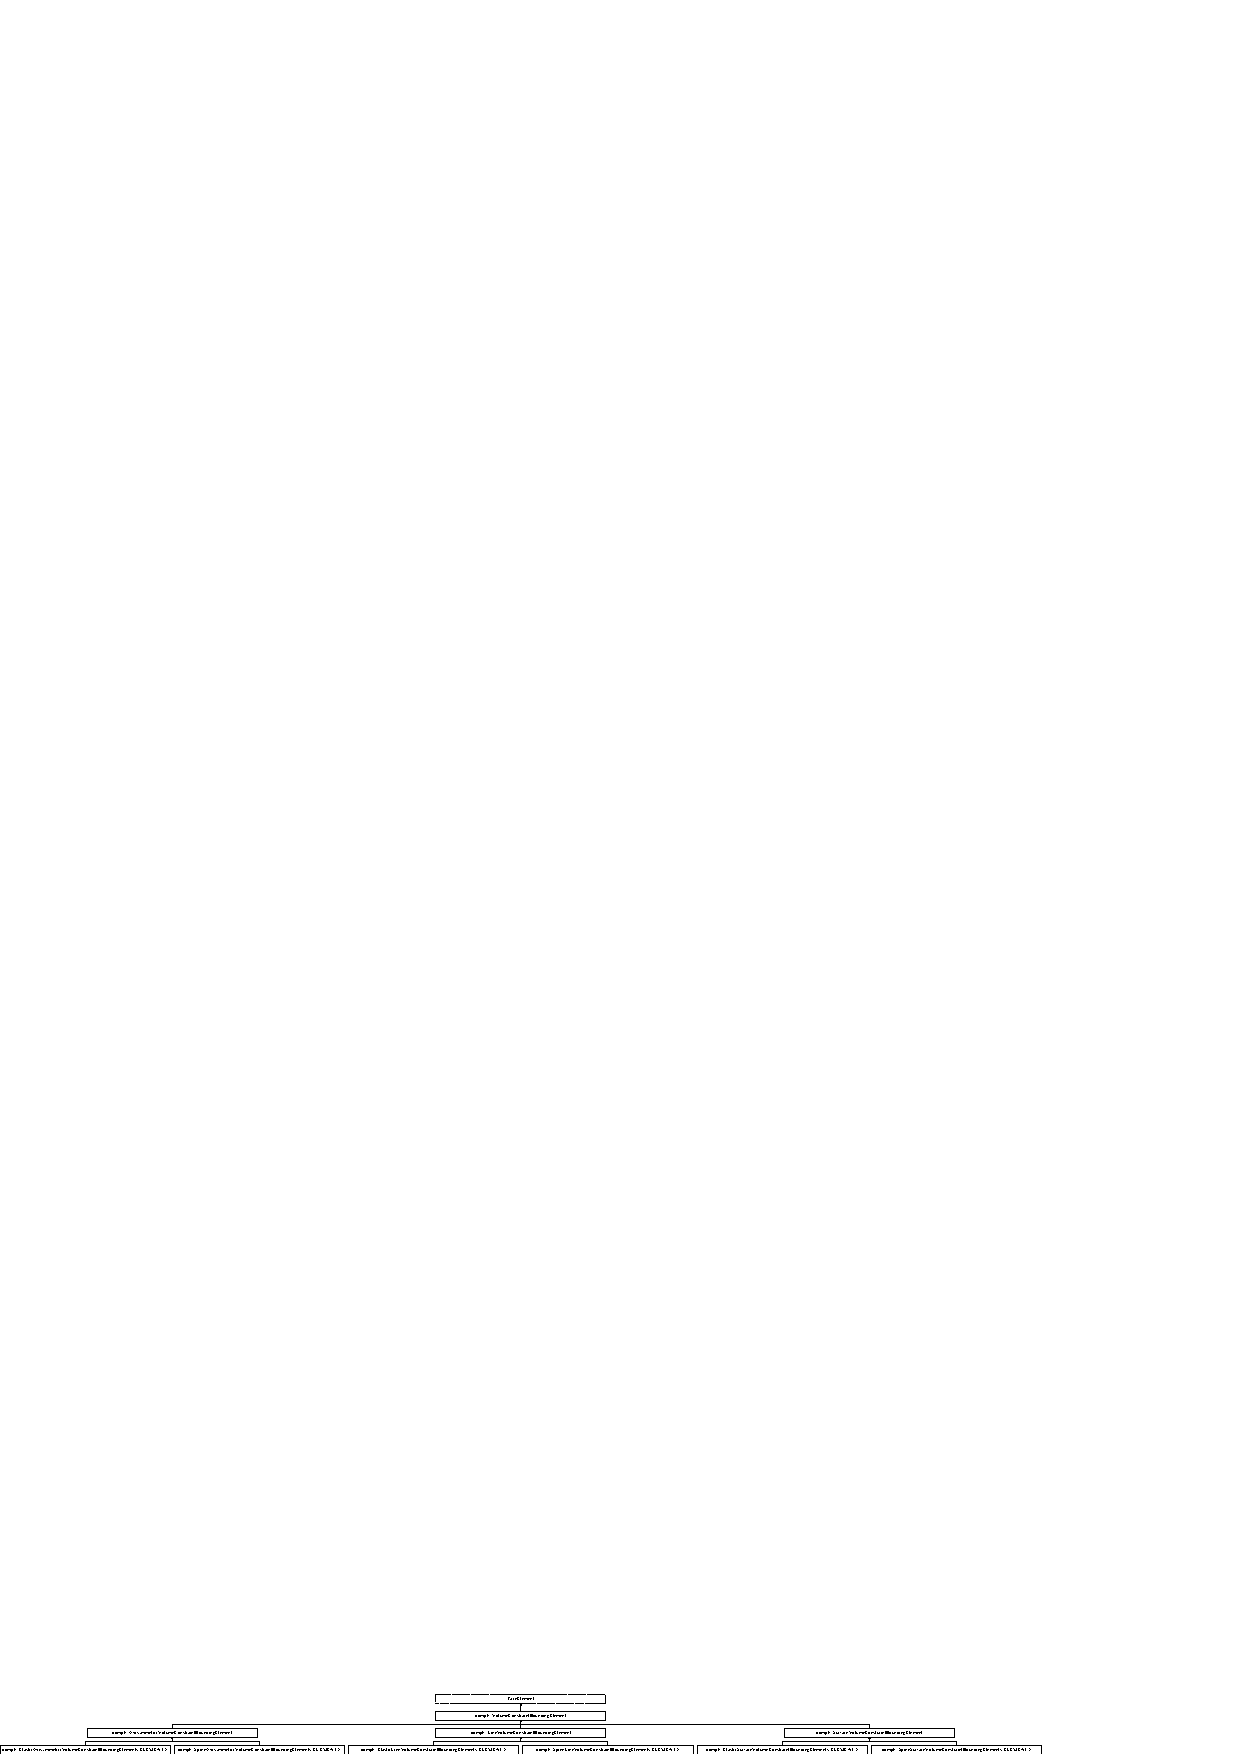
\includegraphics[height=1.238938cm]{classoomph_1_1VolumeConstraintBoundingElement}
\end{center}
\end{figure}
\subsection*{Public Member Functions}
\begin{DoxyCompactItemize}
\item 
\hyperlink{classoomph_1_1VolumeConstraintBoundingElement_a423139995a5543fda59d36cf230edb44}{Volume\+Constraint\+Bounding\+Element} ()
\begin{DoxyCompactList}\small\item\em Constructor initialise the boolean flag We expect the traded pressure data to be stored externally. \end{DoxyCompactList}\item 
\hyperlink{classoomph_1_1VolumeConstraintBoundingElement_a6a54150611ce06f05ea47ba99cf9e132}{$\sim$\+Volume\+Constraint\+Bounding\+Element} ()
\begin{DoxyCompactList}\small\item\em Empty Destructor. \end{DoxyCompactList}\item 
void \hyperlink{classoomph_1_1VolumeConstraintBoundingElement_a0ae62125450a5d203bc6d26b0d24be22}{fill\+\_\+in\+\_\+contribution\+\_\+to\+\_\+residuals} (\hyperlink{classoomph_1_1Vector}{Vector}$<$ double $>$ \&residuals)
\begin{DoxyCompactList}\small\item\em Fill in contribution to residuals and Jacobian. \end{DoxyCompactList}\item 
void \hyperlink{classoomph_1_1VolumeConstraintBoundingElement_a310fbaeb9a024406e4f769886e9f902a}{set\+\_\+volume\+\_\+constraint\+\_\+element} (\hyperlink{classoomph_1_1VolumeConstraintElement}{Volume\+Constraint\+Element} $\ast$const \&vol\+\_\+constraint\+\_\+el\+\_\+pt, const bool \&check\+\_\+nodal\+\_\+data=true)
\begin{DoxyCompactList}\small\item\em Set the \char`\"{}master\char`\"{} volume constraint element The setup here is a bit more complicated than one might expect because if an internal pressure on a boundary is hijacked in Taylor\+Hood elements then that the \char`\"{}traded\char`\"{} value may already be stored as nodal data in this element. This causes no problems apart from when running with P\+A\+R\+A\+N\+O\+ID in which case the resulting repeated local equation numbers are spotted and an error is thrown. The check is a finite amount of work and so can be avoided if the boolean flag check\+\_\+nodal\+\_\+data is set to false. \end{DoxyCompactList}\end{DoxyCompactItemize}
\subsection*{Protected Member Functions}
\begin{DoxyCompactItemize}
\item 
int \hyperlink{classoomph_1_1VolumeConstraintBoundingElement_ae5262edeb9cd3bcbc1ae4265b08c7f07}{ptraded\+\_\+local\+\_\+eqn} ()
\begin{DoxyCompactList}\small\item\em The local eqn number for the traded pressure. \end{DoxyCompactList}\item 
virtual void \hyperlink{classoomph_1_1VolumeConstraintBoundingElement_a717f1085709bd8820b8043ff94ecb0c5}{fill\+\_\+in\+\_\+generic\+\_\+residual\+\_\+contribution\+\_\+volume\+\_\+constraint} (\hyperlink{classoomph_1_1Vector}{Vector}$<$ double $>$ \&residuals)=0
\begin{DoxyCompactList}\small\item\em Helper function to fill in contributions to residuals (remember that part of the residual is added by the the associated \hyperlink{classoomph_1_1VolumeConstraintElement}{Volume\+Constraint\+Element}). This is dimension/geometry specific and must be implemented in derived classes for 1D line, 2D surface and axisymmetric fluid boundaries. \end{DoxyCompactList}\end{DoxyCompactItemize}
\subsection*{Protected Attributes}
\begin{DoxyCompactItemize}
\item 
unsigned \hyperlink{classoomph_1_1VolumeConstraintBoundingElement_afd35462188f27b6851416ab49ec5df5a}{Data\+\_\+number\+\_\+of\+\_\+traded\+\_\+pressure}
\begin{DoxyCompactList}\small\item\em The \hyperlink{classoomph_1_1Data}{Data} that contains the traded pressure is usually stored as external \hyperlink{classoomph_1_1Data}{Data} for this element, but may also be nodal \hyperlink{classoomph_1_1Data}{Data} Which \hyperlink{classoomph_1_1Data}{Data} item is it? \end{DoxyCompactList}\item 
unsigned \hyperlink{classoomph_1_1VolumeConstraintBoundingElement_a40f5ebebeaf633515951a2d08060ec15}{Index\+\_\+of\+\_\+traded\+\_\+pressure\+\_\+value}
\item 
bool \hyperlink{classoomph_1_1VolumeConstraintBoundingElement_a8f9aa94f106fd443fa690851a0268720}{Traded\+\_\+pressure\+\_\+stored\+\_\+at\+\_\+node}
\begin{DoxyCompactList}\small\item\em Boolean to indicate whether the traded pressure is stored externally or at a node (this can happen in Taylor-\/\+Hood elements) \end{DoxyCompactList}\end{DoxyCompactItemize}
\subsection*{Additional Inherited Members}


\subsection{Detailed Description}
Base class for interface elements that allow the application of a volume constraint on the region bounded by these elements. The elements must be used together with the associated \hyperlink{classoomph_1_1VolumeConstraintElement}{Volume\+Constraint\+Element} which stores the value of the target volume. Common functionality is provided in this base for storing the external \char`\"{}pressure\char`\"{} value that is traded for the volume constraint. 

Definition at line 200 of file constrained\+\_\+volume\+\_\+elements.\+h.



\subsection{Constructor \& Destructor Documentation}
\mbox{\Hypertarget{classoomph_1_1VolumeConstraintBoundingElement_a423139995a5543fda59d36cf230edb44}\label{classoomph_1_1VolumeConstraintBoundingElement_a423139995a5543fda59d36cf230edb44}} 
\index{oomph\+::\+Volume\+Constraint\+Bounding\+Element@{oomph\+::\+Volume\+Constraint\+Bounding\+Element}!Volume\+Constraint\+Bounding\+Element@{Volume\+Constraint\+Bounding\+Element}}
\index{Volume\+Constraint\+Bounding\+Element@{Volume\+Constraint\+Bounding\+Element}!oomph\+::\+Volume\+Constraint\+Bounding\+Element@{oomph\+::\+Volume\+Constraint\+Bounding\+Element}}
\subsubsection{\texorpdfstring{Volume\+Constraint\+Bounding\+Element()}{VolumeConstraintBoundingElement()}}
{\footnotesize\ttfamily oomph\+::\+Volume\+Constraint\+Bounding\+Element\+::\+Volume\+Constraint\+Bounding\+Element (\begin{DoxyParamCaption}{ }\end{DoxyParamCaption})\hspace{0.3cm}{\ttfamily [inline]}}



Constructor initialise the boolean flag We expect the traded pressure data to be stored externally. 



Definition at line 247 of file constrained\+\_\+volume\+\_\+elements.\+h.

\mbox{\Hypertarget{classoomph_1_1VolumeConstraintBoundingElement_a6a54150611ce06f05ea47ba99cf9e132}\label{classoomph_1_1VolumeConstraintBoundingElement_a6a54150611ce06f05ea47ba99cf9e132}} 
\index{oomph\+::\+Volume\+Constraint\+Bounding\+Element@{oomph\+::\+Volume\+Constraint\+Bounding\+Element}!````~Volume\+Constraint\+Bounding\+Element@{$\sim$\+Volume\+Constraint\+Bounding\+Element}}
\index{````~Volume\+Constraint\+Bounding\+Element@{$\sim$\+Volume\+Constraint\+Bounding\+Element}!oomph\+::\+Volume\+Constraint\+Bounding\+Element@{oomph\+::\+Volume\+Constraint\+Bounding\+Element}}
\subsubsection{\texorpdfstring{$\sim$\+Volume\+Constraint\+Bounding\+Element()}{~VolumeConstraintBoundingElement()}}
{\footnotesize\ttfamily oomph\+::\+Volume\+Constraint\+Bounding\+Element\+::$\sim$\+Volume\+Constraint\+Bounding\+Element (\begin{DoxyParamCaption}{ }\end{DoxyParamCaption})\hspace{0.3cm}{\ttfamily [inline]}}



Empty Destructor. 



Definition at line 251 of file constrained\+\_\+volume\+\_\+elements.\+h.



\subsection{Member Function Documentation}
\mbox{\Hypertarget{classoomph_1_1VolumeConstraintBoundingElement_a0ae62125450a5d203bc6d26b0d24be22}\label{classoomph_1_1VolumeConstraintBoundingElement_a0ae62125450a5d203bc6d26b0d24be22}} 
\index{oomph\+::\+Volume\+Constraint\+Bounding\+Element@{oomph\+::\+Volume\+Constraint\+Bounding\+Element}!fill\+\_\+in\+\_\+contribution\+\_\+to\+\_\+residuals@{fill\+\_\+in\+\_\+contribution\+\_\+to\+\_\+residuals}}
\index{fill\+\_\+in\+\_\+contribution\+\_\+to\+\_\+residuals@{fill\+\_\+in\+\_\+contribution\+\_\+to\+\_\+residuals}!oomph\+::\+Volume\+Constraint\+Bounding\+Element@{oomph\+::\+Volume\+Constraint\+Bounding\+Element}}
\subsubsection{\texorpdfstring{fill\+\_\+in\+\_\+contribution\+\_\+to\+\_\+residuals()}{fill\_in\_contribution\_to\_residuals()}}
{\footnotesize\ttfamily void oomph\+::\+Volume\+Constraint\+Bounding\+Element\+::fill\+\_\+in\+\_\+contribution\+\_\+to\+\_\+residuals (\begin{DoxyParamCaption}\item[{\hyperlink{classoomph_1_1Vector}{Vector}$<$ double $>$ \&}]{residuals }\end{DoxyParamCaption})\hspace{0.3cm}{\ttfamily [inline]}, {\ttfamily [virtual]}}



Fill in contribution to residuals and Jacobian. 



Reimplemented from \hyperlink{classoomph_1_1GeneralisedElement_a310c97f515e8504a48179c0e72c550d7}{oomph\+::\+Generalised\+Element}.



Definition at line 254 of file constrained\+\_\+volume\+\_\+elements.\+h.

\mbox{\Hypertarget{classoomph_1_1VolumeConstraintBoundingElement_a717f1085709bd8820b8043ff94ecb0c5}\label{classoomph_1_1VolumeConstraintBoundingElement_a717f1085709bd8820b8043ff94ecb0c5}} 
\index{oomph\+::\+Volume\+Constraint\+Bounding\+Element@{oomph\+::\+Volume\+Constraint\+Bounding\+Element}!fill\+\_\+in\+\_\+generic\+\_\+residual\+\_\+contribution\+\_\+volume\+\_\+constraint@{fill\+\_\+in\+\_\+generic\+\_\+residual\+\_\+contribution\+\_\+volume\+\_\+constraint}}
\index{fill\+\_\+in\+\_\+generic\+\_\+residual\+\_\+contribution\+\_\+volume\+\_\+constraint@{fill\+\_\+in\+\_\+generic\+\_\+residual\+\_\+contribution\+\_\+volume\+\_\+constraint}!oomph\+::\+Volume\+Constraint\+Bounding\+Element@{oomph\+::\+Volume\+Constraint\+Bounding\+Element}}
\subsubsection{\texorpdfstring{fill\+\_\+in\+\_\+generic\+\_\+residual\+\_\+contribution\+\_\+volume\+\_\+constraint()}{fill\_in\_generic\_residual\_contribution\_volume\_constraint()}}
{\footnotesize\ttfamily virtual void oomph\+::\+Volume\+Constraint\+Bounding\+Element\+::fill\+\_\+in\+\_\+generic\+\_\+residual\+\_\+contribution\+\_\+volume\+\_\+constraint (\begin{DoxyParamCaption}\item[{\hyperlink{classoomph_1_1Vector}{Vector}$<$ double $>$ \&}]{residuals }\end{DoxyParamCaption})\hspace{0.3cm}{\ttfamily [protected]}, {\ttfamily [pure virtual]}}



Helper function to fill in contributions to residuals (remember that part of the residual is added by the the associated \hyperlink{classoomph_1_1VolumeConstraintElement}{Volume\+Constraint\+Element}). This is dimension/geometry specific and must be implemented in derived classes for 1D line, 2D surface and axisymmetric fluid boundaries. 



Implemented in \hyperlink{classoomph_1_1SurfaceVolumeConstraintBoundingElement_a5813fa65063eb55a5b264539d77cac88}{oomph\+::\+Surface\+Volume\+Constraint\+Bounding\+Element}, \hyperlink{classoomph_1_1AxisymmetricVolumeConstraintBoundingElement_a2a3f3b86079f27d52679f357f5276d91}{oomph\+::\+Axisymmetric\+Volume\+Constraint\+Bounding\+Element}, and \hyperlink{classoomph_1_1LineVolumeConstraintBoundingElement_a03145a064e559d786f730c85000f9fb4}{oomph\+::\+Line\+Volume\+Constraint\+Bounding\+Element}.

\mbox{\Hypertarget{classoomph_1_1VolumeConstraintBoundingElement_ae5262edeb9cd3bcbc1ae4265b08c7f07}\label{classoomph_1_1VolumeConstraintBoundingElement_ae5262edeb9cd3bcbc1ae4265b08c7f07}} 
\index{oomph\+::\+Volume\+Constraint\+Bounding\+Element@{oomph\+::\+Volume\+Constraint\+Bounding\+Element}!ptraded\+\_\+local\+\_\+eqn@{ptraded\+\_\+local\+\_\+eqn}}
\index{ptraded\+\_\+local\+\_\+eqn@{ptraded\+\_\+local\+\_\+eqn}!oomph\+::\+Volume\+Constraint\+Bounding\+Element@{oomph\+::\+Volume\+Constraint\+Bounding\+Element}}
\subsubsection{\texorpdfstring{ptraded\+\_\+local\+\_\+eqn()}{ptraded\_local\_eqn()}}
{\footnotesize\ttfamily int oomph\+::\+Volume\+Constraint\+Bounding\+Element\+::ptraded\+\_\+local\+\_\+eqn (\begin{DoxyParamCaption}{ }\end{DoxyParamCaption})\hspace{0.3cm}{\ttfamily [inline]}, {\ttfamily [protected]}}



The local eqn number for the traded pressure. 



Definition at line 220 of file constrained\+\_\+volume\+\_\+elements.\+h.



References oomph\+::\+Generalised\+Element\+::external\+\_\+local\+\_\+eqn().

\mbox{\Hypertarget{classoomph_1_1VolumeConstraintBoundingElement_a310fbaeb9a024406e4f769886e9f902a}\label{classoomph_1_1VolumeConstraintBoundingElement_a310fbaeb9a024406e4f769886e9f902a}} 
\index{oomph\+::\+Volume\+Constraint\+Bounding\+Element@{oomph\+::\+Volume\+Constraint\+Bounding\+Element}!set\+\_\+volume\+\_\+constraint\+\_\+element@{set\+\_\+volume\+\_\+constraint\+\_\+element}}
\index{set\+\_\+volume\+\_\+constraint\+\_\+element@{set\+\_\+volume\+\_\+constraint\+\_\+element}!oomph\+::\+Volume\+Constraint\+Bounding\+Element@{oomph\+::\+Volume\+Constraint\+Bounding\+Element}}
\subsubsection{\texorpdfstring{set\+\_\+volume\+\_\+constraint\+\_\+element()}{set\_volume\_constraint\_element()}}
{\footnotesize\ttfamily void oomph\+::\+Volume\+Constraint\+Bounding\+Element\+::set\+\_\+volume\+\_\+constraint\+\_\+element (\begin{DoxyParamCaption}\item[{\hyperlink{classoomph_1_1VolumeConstraintElement}{Volume\+Constraint\+Element} $\ast$const \&}]{vol\+\_\+constraint\+\_\+el\+\_\+pt,  }\item[{const bool \&}]{check\+\_\+nodal\+\_\+data = {\ttfamily true} }\end{DoxyParamCaption})\hspace{0.3cm}{\ttfamily [inline]}}



Set the \char`\"{}master\char`\"{} volume constraint element The setup here is a bit more complicated than one might expect because if an internal pressure on a boundary is hijacked in Taylor\+Hood elements then that the \char`\"{}traded\char`\"{} value may already be stored as nodal data in this element. This causes no problems apart from when running with P\+A\+R\+A\+N\+O\+ID in which case the resulting repeated local equation numbers are spotted and an error is thrown. The check is a finite amount of work and so can be avoided if the boolean flag check\+\_\+nodal\+\_\+data is set to false. 



Definition at line 270 of file constrained\+\_\+volume\+\_\+elements.\+h.



References oomph\+::\+Generalised\+Element\+::add\+\_\+external\+\_\+data(), oomph\+::\+Data\+::eqn\+\_\+number\+\_\+pt(), i, oomph\+::\+Volume\+Constraint\+Element\+::index\+\_\+of\+\_\+traded\+\_\+pressure(), oomph\+::\+Data\+::nvalue(), and oomph\+::\+Volume\+Constraint\+Element\+::p\+\_\+traded\+\_\+data\+\_\+pt().



\subsection{Member Data Documentation}
\mbox{\Hypertarget{classoomph_1_1VolumeConstraintBoundingElement_afd35462188f27b6851416ab49ec5df5a}\label{classoomph_1_1VolumeConstraintBoundingElement_afd35462188f27b6851416ab49ec5df5a}} 
\index{oomph\+::\+Volume\+Constraint\+Bounding\+Element@{oomph\+::\+Volume\+Constraint\+Bounding\+Element}!Data\+\_\+number\+\_\+of\+\_\+traded\+\_\+pressure@{Data\+\_\+number\+\_\+of\+\_\+traded\+\_\+pressure}}
\index{Data\+\_\+number\+\_\+of\+\_\+traded\+\_\+pressure@{Data\+\_\+number\+\_\+of\+\_\+traded\+\_\+pressure}!oomph\+::\+Volume\+Constraint\+Bounding\+Element@{oomph\+::\+Volume\+Constraint\+Bounding\+Element}}
\subsubsection{\texorpdfstring{Data\+\_\+number\+\_\+of\+\_\+traded\+\_\+pressure}{Data\_number\_of\_traded\_pressure}}
{\footnotesize\ttfamily unsigned oomph\+::\+Volume\+Constraint\+Bounding\+Element\+::\+Data\+\_\+number\+\_\+of\+\_\+traded\+\_\+pressure\hspace{0.3cm}{\ttfamily [protected]}}



The \hyperlink{classoomph_1_1Data}{Data} that contains the traded pressure is usually stored as external \hyperlink{classoomph_1_1Data}{Data} for this element, but may also be nodal \hyperlink{classoomph_1_1Data}{Data} Which \hyperlink{classoomph_1_1Data}{Data} item is it? 



Definition at line 208 of file constrained\+\_\+volume\+\_\+elements.\+h.

\mbox{\Hypertarget{classoomph_1_1VolumeConstraintBoundingElement_a40f5ebebeaf633515951a2d08060ec15}\label{classoomph_1_1VolumeConstraintBoundingElement_a40f5ebebeaf633515951a2d08060ec15}} 
\index{oomph\+::\+Volume\+Constraint\+Bounding\+Element@{oomph\+::\+Volume\+Constraint\+Bounding\+Element}!Index\+\_\+of\+\_\+traded\+\_\+pressure\+\_\+value@{Index\+\_\+of\+\_\+traded\+\_\+pressure\+\_\+value}}
\index{Index\+\_\+of\+\_\+traded\+\_\+pressure\+\_\+value@{Index\+\_\+of\+\_\+traded\+\_\+pressure\+\_\+value}!oomph\+::\+Volume\+Constraint\+Bounding\+Element@{oomph\+::\+Volume\+Constraint\+Bounding\+Element}}
\subsubsection{\texorpdfstring{Index\+\_\+of\+\_\+traded\+\_\+pressure\+\_\+value}{Index\_of\_traded\_pressure\_value}}
{\footnotesize\ttfamily unsigned oomph\+::\+Volume\+Constraint\+Bounding\+Element\+::\+Index\+\_\+of\+\_\+traded\+\_\+pressure\+\_\+value\hspace{0.3cm}{\ttfamily [protected]}}

Index of the value in traded pressure data that corresponds to the traded pressure 

Definition at line 212 of file constrained\+\_\+volume\+\_\+elements.\+h.

\mbox{\Hypertarget{classoomph_1_1VolumeConstraintBoundingElement_a8f9aa94f106fd443fa690851a0268720}\label{classoomph_1_1VolumeConstraintBoundingElement_a8f9aa94f106fd443fa690851a0268720}} 
\index{oomph\+::\+Volume\+Constraint\+Bounding\+Element@{oomph\+::\+Volume\+Constraint\+Bounding\+Element}!Traded\+\_\+pressure\+\_\+stored\+\_\+at\+\_\+node@{Traded\+\_\+pressure\+\_\+stored\+\_\+at\+\_\+node}}
\index{Traded\+\_\+pressure\+\_\+stored\+\_\+at\+\_\+node@{Traded\+\_\+pressure\+\_\+stored\+\_\+at\+\_\+node}!oomph\+::\+Volume\+Constraint\+Bounding\+Element@{oomph\+::\+Volume\+Constraint\+Bounding\+Element}}
\subsubsection{\texorpdfstring{Traded\+\_\+pressure\+\_\+stored\+\_\+at\+\_\+node}{Traded\_pressure\_stored\_at\_node}}
{\footnotesize\ttfamily bool oomph\+::\+Volume\+Constraint\+Bounding\+Element\+::\+Traded\+\_\+pressure\+\_\+stored\+\_\+at\+\_\+node\hspace{0.3cm}{\ttfamily [protected]}}



Boolean to indicate whether the traded pressure is stored externally or at a node (this can happen in Taylor-\/\+Hood elements) 



Definition at line 217 of file constrained\+\_\+volume\+\_\+elements.\+h.



The documentation for this class was generated from the following file\+:\begin{DoxyCompactItemize}
\item 
\hyperlink{constrained__volume__elements_8h}{constrained\+\_\+volume\+\_\+elements.\+h}\end{DoxyCompactItemize}

\hypertarget{classoomph_1_1VolumeConstraintElement}{}\section{oomph\+:\+:Volume\+Constraint\+Element Class Reference}
\label{classoomph_1_1VolumeConstraintElement}\index{oomph\+::\+Volume\+Constraint\+Element@{oomph\+::\+Volume\+Constraint\+Element}}


{\ttfamily \#include $<$constrained\+\_\+volume\+\_\+elements.\+h$>$}

Inheritance diagram for oomph\+:\+:Volume\+Constraint\+Element\+:\begin{figure}[H]
\begin{center}
\leavevmode
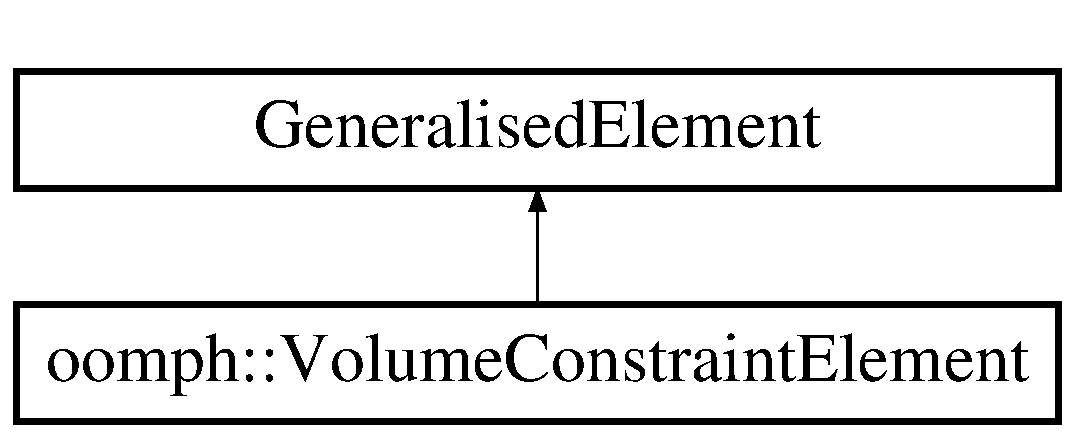
\includegraphics[height=2.000000cm]{classoomph_1_1VolumeConstraintElement}
\end{center}
\end{figure}
\subsection*{Public Member Functions}
\begin{DoxyCompactItemize}
\item 
\hyperlink{classoomph_1_1VolumeConstraintElement_a641eea5633b1ddd2d9f79e5731947660}{Volume\+Constraint\+Element} (double $\ast$prescribed\+\_\+volume\+\_\+pt)
\begin{DoxyCompactList}\small\item\em Constructor\+: Pass pointer to target volume. \char`\"{}\+Pressure\char`\"{} value that \char`\"{}traded\char`\"{} for the volume contraint is created internally (as a Data item with a single pressure value) \end{DoxyCompactList}\item 
\hyperlink{classoomph_1_1VolumeConstraintElement_adc0fc16f4fc708fb09d70cb791a6c6b9}{Volume\+Constraint\+Element} (double $\ast$prescribed\+\_\+volume\+\_\+pt, Data $\ast$\hyperlink{classoomph_1_1VolumeConstraintElement_a60d17437a54648747c956b7a7067c592}{p\+\_\+traded\+\_\+data\+\_\+pt}, const unsigned \&\hyperlink{classoomph_1_1VolumeConstraintElement_ada831157effca052df0fae723c21c426}{index\+\_\+of\+\_\+traded\+\_\+pressure})
\begin{DoxyCompactList}\small\item\em Constructor\+: Pass pointer to target volume, pointer to Data item whose value specified by index\+\_\+of\+\_\+traded\+\_\+pressure represents the \char`\"{}\+Pressure\char`\"{} value that \char`\"{}traded\char`\"{} for the volume contraint. The Data is stored as external Data for this element. \end{DoxyCompactList}\item 
\hyperlink{classoomph_1_1VolumeConstraintElement_a160b5edcca9ce59bbd6afe90c3729bbb}{$\sim$\+Volume\+Constraint\+Element} ()
\begin{DoxyCompactList}\small\item\em Empty destructor. \end{DoxyCompactList}\item 
Data $\ast$ \hyperlink{classoomph_1_1VolumeConstraintElement_a60d17437a54648747c956b7a7067c592}{p\+\_\+traded\+\_\+data\+\_\+pt} ()
\begin{DoxyCompactList}\small\item\em Access to Data that contains the traded pressure. \end{DoxyCompactList}\item 
double \hyperlink{classoomph_1_1VolumeConstraintElement_aab138c0a3af1e72089d5bed31a633974}{p\+\_\+traded} ()
\begin{DoxyCompactList}\small\item\em Return the traded pressure value. \end{DoxyCompactList}\item 
unsigned \hyperlink{classoomph_1_1VolumeConstraintElement_ada831157effca052df0fae723c21c426}{index\+\_\+of\+\_\+traded\+\_\+pressure} ()
\begin{DoxyCompactList}\small\item\em Return the index of Data object at which the traded pressure is stored. \end{DoxyCompactList}\item 
void \hyperlink{classoomph_1_1VolumeConstraintElement_a15162ac88c571496cc4f9ab5afa51c52}{fill\+\_\+in\+\_\+contribution\+\_\+to\+\_\+residuals} (Vector$<$ double $>$ \&residuals)
\begin{DoxyCompactList}\small\item\em Fill in the residuals for the volume constraint. \end{DoxyCompactList}\item 
void \hyperlink{classoomph_1_1VolumeConstraintElement_a725474b173e3887f5f7e025acf768b28}{fill\+\_\+in\+\_\+contribution\+\_\+to\+\_\+jacobian} (Vector$<$ double $>$ \&residuals, Dense\+Matrix$<$ double $>$ \&jacobian)
\begin{DoxyCompactList}\small\item\em Fill in the residuals and jacobian for the volume constraint. \end{DoxyCompactList}\item 
void \hyperlink{classoomph_1_1VolumeConstraintElement_af2a5a59f7fa5f2570d2d490f3610de61}{fill\+\_\+in\+\_\+contribution\+\_\+to\+\_\+jacobian\+\_\+and\+\_\+mass\+\_\+matrix} (Vector$<$ double $>$ \&residuals, Dense\+Matrix$<$ double $>$ \&jacobian, Dense\+Matrix$<$ double $>$ \&mass\+\_\+matrix)
\begin{DoxyCompactList}\small\item\em Fill in the residuals, jacobian and mass matrix for the volume constraint. \end{DoxyCompactList}\end{DoxyCompactItemize}
\subsection*{Private Member Functions}
\begin{DoxyCompactItemize}
\item 
int \hyperlink{classoomph_1_1VolumeConstraintElement_ad0dedf705ccfb713848ad960bf1b901d}{ptraded\+\_\+local\+\_\+eqn} ()
\begin{DoxyCompactList}\small\item\em The local eqn number for the traded pressure. \end{DoxyCompactList}\item 
void \hyperlink{classoomph_1_1VolumeConstraintElement_a1139fafaca2b784c0561457606cc307e}{fill\+\_\+in\+\_\+generic\+\_\+contribution\+\_\+to\+\_\+residuals\+\_\+volume\+\_\+constraint} (Vector$<$ double $>$ \&residuals)
\begin{DoxyCompactList}\small\item\em Fill in the residuals for the volume constraint. \end{DoxyCompactList}\end{DoxyCompactItemize}
\subsection*{Private Attributes}
\begin{DoxyCompactItemize}
\item 
double $\ast$ \hyperlink{classoomph_1_1VolumeConstraintElement_ae109f08c27d29b0749b46285703cb16f}{Prescribed\+\_\+volume\+\_\+pt}
\begin{DoxyCompactList}\small\item\em Pointer to the desired value of the volume. \end{DoxyCompactList}\item 
unsigned \hyperlink{classoomph_1_1VolumeConstraintElement_a51d3b504e02842219a50f043e8cd81f3}{External\+\_\+or\+\_\+internal\+\_\+data\+\_\+index\+\_\+of\+\_\+traded\+\_\+pressure}
\begin{DoxyCompactList}\small\item\em The Data that contains the traded pressure is stored as external or internal Data for the element. What is its index in these containers? \end{DoxyCompactList}\item 
bool \hyperlink{classoomph_1_1VolumeConstraintElement_ac4275cd18ae758b71ba4191aa2ff9a28}{Traded\+\_\+pressure\+\_\+stored\+\_\+as\+\_\+internal\+\_\+data}
\begin{DoxyCompactList}\small\item\em The Data that contains the traded pressure is stored as external or internal Data for the element. Which one? \end{DoxyCompactList}\item 
unsigned \hyperlink{classoomph_1_1VolumeConstraintElement_a4f2dd24f0ae52cc665daab425bf94745}{Index\+\_\+of\+\_\+traded\+\_\+pressure\+\_\+value}
\end{DoxyCompactItemize}


\subsection{Detailed Description}
A class that is used to implement the constraint that the fluid volume in a region bounded by associated Face\+Elements (attached, e.\+g., to the mesh boundaries that enclose a bubble) must take a specific value. This Generalised\+Element is used only to store the desired volume and a pointer to the (usually pressure) freedom that must be traded for the volume constraint. 

Definition at line 70 of file constrained\+\_\+volume\+\_\+elements.\+h.



\subsection{Constructor \& Destructor Documentation}
\mbox{\Hypertarget{classoomph_1_1VolumeConstraintElement_a641eea5633b1ddd2d9f79e5731947660}\label{classoomph_1_1VolumeConstraintElement_a641eea5633b1ddd2d9f79e5731947660}} 
\index{oomph\+::\+Volume\+Constraint\+Element@{oomph\+::\+Volume\+Constraint\+Element}!Volume\+Constraint\+Element@{Volume\+Constraint\+Element}}
\index{Volume\+Constraint\+Element@{Volume\+Constraint\+Element}!oomph\+::\+Volume\+Constraint\+Element@{oomph\+::\+Volume\+Constraint\+Element}}
\subsubsection{\texorpdfstring{Volume\+Constraint\+Element()}{VolumeConstraintElement()}\hspace{0.1cm}{\footnotesize\ttfamily [1/2]}}
{\footnotesize\ttfamily oomph\+::\+Volume\+Constraint\+Element\+::\+Volume\+Constraint\+Element (\begin{DoxyParamCaption}\item[{double $\ast$}]{prescribed\+\_\+volume\+\_\+pt }\end{DoxyParamCaption})}



Constructor\+: Pass pointer to target volume. \char`\"{}\+Pressure\char`\"{} value that \char`\"{}traded\char`\"{} for the volume contraint is created internally (as a Data item with a single pressure value) 



Definition at line 65 of file constrained\+\_\+volume\+\_\+elements.\+cc.



References External\+\_\+or\+\_\+internal\+\_\+data\+\_\+index\+\_\+of\+\_\+traded\+\_\+pressure, Index\+\_\+of\+\_\+traded\+\_\+pressure\+\_\+value, Prescribed\+\_\+volume\+\_\+pt, and Traded\+\_\+pressure\+\_\+stored\+\_\+as\+\_\+internal\+\_\+data.



Referenced by ptraded\+\_\+local\+\_\+eqn().

\mbox{\Hypertarget{classoomph_1_1VolumeConstraintElement_adc0fc16f4fc708fb09d70cb791a6c6b9}\label{classoomph_1_1VolumeConstraintElement_adc0fc16f4fc708fb09d70cb791a6c6b9}} 
\index{oomph\+::\+Volume\+Constraint\+Element@{oomph\+::\+Volume\+Constraint\+Element}!Volume\+Constraint\+Element@{Volume\+Constraint\+Element}}
\index{Volume\+Constraint\+Element@{Volume\+Constraint\+Element}!oomph\+::\+Volume\+Constraint\+Element@{oomph\+::\+Volume\+Constraint\+Element}}
\subsubsection{\texorpdfstring{Volume\+Constraint\+Element()}{VolumeConstraintElement()}\hspace{0.1cm}{\footnotesize\ttfamily [2/2]}}
{\footnotesize\ttfamily oomph\+::\+Volume\+Constraint\+Element\+::\+Volume\+Constraint\+Element (\begin{DoxyParamCaption}\item[{double $\ast$}]{prescribed\+\_\+volume\+\_\+pt,  }\item[{Data $\ast$}]{p\+\_\+traded\+\_\+data\+\_\+pt,  }\item[{const unsigned \&}]{index\+\_\+of\+\_\+traded\+\_\+pressure }\end{DoxyParamCaption})}



Constructor\+: Pass pointer to target volume, pointer to Data item whose value specified by index\+\_\+of\+\_\+traded\+\_\+pressure represents the \char`\"{}\+Pressure\char`\"{} value that \char`\"{}traded\char`\"{} for the volume contraint. The Data is stored as external Data for this element. 



Definition at line 88 of file constrained\+\_\+volume\+\_\+elements.\+cc.



References External\+\_\+or\+\_\+internal\+\_\+data\+\_\+index\+\_\+of\+\_\+traded\+\_\+pressure, oomph\+::\+Line\+Volume\+Constraint\+Bounding\+Element\+::fill\+\_\+in\+\_\+generic\+\_\+residual\+\_\+contribution\+\_\+volume\+\_\+constraint(), index\+\_\+of\+\_\+traded\+\_\+pressure(), Index\+\_\+of\+\_\+traded\+\_\+pressure\+\_\+value, Prescribed\+\_\+volume\+\_\+pt, and Traded\+\_\+pressure\+\_\+stored\+\_\+as\+\_\+internal\+\_\+data.

\mbox{\Hypertarget{classoomph_1_1VolumeConstraintElement_a160b5edcca9ce59bbd6afe90c3729bbb}\label{classoomph_1_1VolumeConstraintElement_a160b5edcca9ce59bbd6afe90c3729bbb}} 
\index{oomph\+::\+Volume\+Constraint\+Element@{oomph\+::\+Volume\+Constraint\+Element}!````~Volume\+Constraint\+Element@{$\sim$\+Volume\+Constraint\+Element}}
\index{````~Volume\+Constraint\+Element@{$\sim$\+Volume\+Constraint\+Element}!oomph\+::\+Volume\+Constraint\+Element@{oomph\+::\+Volume\+Constraint\+Element}}
\subsubsection{\texorpdfstring{$\sim$\+Volume\+Constraint\+Element()}{~VolumeConstraintElement()}}
{\footnotesize\ttfamily oomph\+::\+Volume\+Constraint\+Element\+::$\sim$\+Volume\+Constraint\+Element (\begin{DoxyParamCaption}{ }\end{DoxyParamCaption})\hspace{0.3cm}{\ttfamily [inline]}}



Empty destructor. 



Definition at line 130 of file constrained\+\_\+volume\+\_\+elements.\+h.



\subsection{Member Function Documentation}
\mbox{\Hypertarget{classoomph_1_1VolumeConstraintElement_a725474b173e3887f5f7e025acf768b28}\label{classoomph_1_1VolumeConstraintElement_a725474b173e3887f5f7e025acf768b28}} 
\index{oomph\+::\+Volume\+Constraint\+Element@{oomph\+::\+Volume\+Constraint\+Element}!fill\+\_\+in\+\_\+contribution\+\_\+to\+\_\+jacobian@{fill\+\_\+in\+\_\+contribution\+\_\+to\+\_\+jacobian}}
\index{fill\+\_\+in\+\_\+contribution\+\_\+to\+\_\+jacobian@{fill\+\_\+in\+\_\+contribution\+\_\+to\+\_\+jacobian}!oomph\+::\+Volume\+Constraint\+Element@{oomph\+::\+Volume\+Constraint\+Element}}
\subsubsection{\texorpdfstring{fill\+\_\+in\+\_\+contribution\+\_\+to\+\_\+jacobian()}{fill\_in\_contribution\_to\_jacobian()}}
{\footnotesize\ttfamily void oomph\+::\+Volume\+Constraint\+Element\+::fill\+\_\+in\+\_\+contribution\+\_\+to\+\_\+jacobian (\begin{DoxyParamCaption}\item[{Vector$<$ double $>$ \&}]{residuals,  }\item[{Dense\+Matrix$<$ double $>$ \&}]{jacobian }\end{DoxyParamCaption})\hspace{0.3cm}{\ttfamily [inline]}}



Fill in the residuals and jacobian for the volume constraint. 



Definition at line 164 of file constrained\+\_\+volume\+\_\+elements.\+h.



References fill\+\_\+in\+\_\+generic\+\_\+contribution\+\_\+to\+\_\+residuals\+\_\+volume\+\_\+constraint().

\mbox{\Hypertarget{classoomph_1_1VolumeConstraintElement_af2a5a59f7fa5f2570d2d490f3610de61}\label{classoomph_1_1VolumeConstraintElement_af2a5a59f7fa5f2570d2d490f3610de61}} 
\index{oomph\+::\+Volume\+Constraint\+Element@{oomph\+::\+Volume\+Constraint\+Element}!fill\+\_\+in\+\_\+contribution\+\_\+to\+\_\+jacobian\+\_\+and\+\_\+mass\+\_\+matrix@{fill\+\_\+in\+\_\+contribution\+\_\+to\+\_\+jacobian\+\_\+and\+\_\+mass\+\_\+matrix}}
\index{fill\+\_\+in\+\_\+contribution\+\_\+to\+\_\+jacobian\+\_\+and\+\_\+mass\+\_\+matrix@{fill\+\_\+in\+\_\+contribution\+\_\+to\+\_\+jacobian\+\_\+and\+\_\+mass\+\_\+matrix}!oomph\+::\+Volume\+Constraint\+Element@{oomph\+::\+Volume\+Constraint\+Element}}
\subsubsection{\texorpdfstring{fill\+\_\+in\+\_\+contribution\+\_\+to\+\_\+jacobian\+\_\+and\+\_\+mass\+\_\+matrix()}{fill\_in\_contribution\_to\_jacobian\_and\_mass\_matrix()}}
{\footnotesize\ttfamily void oomph\+::\+Volume\+Constraint\+Element\+::fill\+\_\+in\+\_\+contribution\+\_\+to\+\_\+jacobian\+\_\+and\+\_\+mass\+\_\+matrix (\begin{DoxyParamCaption}\item[{Vector$<$ double $>$ \&}]{residuals,  }\item[{Dense\+Matrix$<$ double $>$ \&}]{jacobian,  }\item[{Dense\+Matrix$<$ double $>$ \&}]{mass\+\_\+matrix }\end{DoxyParamCaption})\hspace{0.3cm}{\ttfamily [inline]}}



Fill in the residuals, jacobian and mass matrix for the volume constraint. 



Definition at line 174 of file constrained\+\_\+volume\+\_\+elements.\+h.



References fill\+\_\+in\+\_\+generic\+\_\+contribution\+\_\+to\+\_\+residuals\+\_\+volume\+\_\+constraint().

\mbox{\Hypertarget{classoomph_1_1VolumeConstraintElement_a15162ac88c571496cc4f9ab5afa51c52}\label{classoomph_1_1VolumeConstraintElement_a15162ac88c571496cc4f9ab5afa51c52}} 
\index{oomph\+::\+Volume\+Constraint\+Element@{oomph\+::\+Volume\+Constraint\+Element}!fill\+\_\+in\+\_\+contribution\+\_\+to\+\_\+residuals@{fill\+\_\+in\+\_\+contribution\+\_\+to\+\_\+residuals}}
\index{fill\+\_\+in\+\_\+contribution\+\_\+to\+\_\+residuals@{fill\+\_\+in\+\_\+contribution\+\_\+to\+\_\+residuals}!oomph\+::\+Volume\+Constraint\+Element@{oomph\+::\+Volume\+Constraint\+Element}}
\subsubsection{\texorpdfstring{fill\+\_\+in\+\_\+contribution\+\_\+to\+\_\+residuals()}{fill\_in\_contribution\_to\_residuals()}}
{\footnotesize\ttfamily void oomph\+::\+Volume\+Constraint\+Element\+::fill\+\_\+in\+\_\+contribution\+\_\+to\+\_\+residuals (\begin{DoxyParamCaption}\item[{Vector$<$ double $>$ \&}]{residuals }\end{DoxyParamCaption})\hspace{0.3cm}{\ttfamily [inline]}}



Fill in the residuals for the volume constraint. 



Definition at line 157 of file constrained\+\_\+volume\+\_\+elements.\+h.



References fill\+\_\+in\+\_\+generic\+\_\+contribution\+\_\+to\+\_\+residuals\+\_\+volume\+\_\+constraint().

\mbox{\Hypertarget{classoomph_1_1VolumeConstraintElement_a1139fafaca2b784c0561457606cc307e}\label{classoomph_1_1VolumeConstraintElement_a1139fafaca2b784c0561457606cc307e}} 
\index{oomph\+::\+Volume\+Constraint\+Element@{oomph\+::\+Volume\+Constraint\+Element}!fill\+\_\+in\+\_\+generic\+\_\+contribution\+\_\+to\+\_\+residuals\+\_\+volume\+\_\+constraint@{fill\+\_\+in\+\_\+generic\+\_\+contribution\+\_\+to\+\_\+residuals\+\_\+volume\+\_\+constraint}}
\index{fill\+\_\+in\+\_\+generic\+\_\+contribution\+\_\+to\+\_\+residuals\+\_\+volume\+\_\+constraint@{fill\+\_\+in\+\_\+generic\+\_\+contribution\+\_\+to\+\_\+residuals\+\_\+volume\+\_\+constraint}!oomph\+::\+Volume\+Constraint\+Element@{oomph\+::\+Volume\+Constraint\+Element}}
\subsubsection{\texorpdfstring{fill\+\_\+in\+\_\+generic\+\_\+contribution\+\_\+to\+\_\+residuals\+\_\+volume\+\_\+constraint()}{fill\_in\_generic\_contribution\_to\_residuals\_volume\_constraint()}}
{\footnotesize\ttfamily void oomph\+::\+Volume\+Constraint\+Element\+::fill\+\_\+in\+\_\+generic\+\_\+contribution\+\_\+to\+\_\+residuals\+\_\+volume\+\_\+constraint (\begin{DoxyParamCaption}\item[{Vector$<$ double $>$ \&}]{residuals }\end{DoxyParamCaption})\hspace{0.3cm}{\ttfamily [private]}}



Fill in the residuals for the volume constraint. 



Definition at line 43 of file constrained\+\_\+volume\+\_\+elements.\+cc.



References Prescribed\+\_\+volume\+\_\+pt, and ptraded\+\_\+local\+\_\+eqn().



Referenced by fill\+\_\+in\+\_\+contribution\+\_\+to\+\_\+jacobian(), fill\+\_\+in\+\_\+contribution\+\_\+to\+\_\+jacobian\+\_\+and\+\_\+mass\+\_\+matrix(), fill\+\_\+in\+\_\+contribution\+\_\+to\+\_\+residuals(), and ptraded\+\_\+local\+\_\+eqn().

\mbox{\Hypertarget{classoomph_1_1VolumeConstraintElement_ada831157effca052df0fae723c21c426}\label{classoomph_1_1VolumeConstraintElement_ada831157effca052df0fae723c21c426}} 
\index{oomph\+::\+Volume\+Constraint\+Element@{oomph\+::\+Volume\+Constraint\+Element}!index\+\_\+of\+\_\+traded\+\_\+pressure@{index\+\_\+of\+\_\+traded\+\_\+pressure}}
\index{index\+\_\+of\+\_\+traded\+\_\+pressure@{index\+\_\+of\+\_\+traded\+\_\+pressure}!oomph\+::\+Volume\+Constraint\+Element@{oomph\+::\+Volume\+Constraint\+Element}}
\subsubsection{\texorpdfstring{index\+\_\+of\+\_\+traded\+\_\+pressure()}{index\_of\_traded\_pressure()}}
{\footnotesize\ttfamily unsigned oomph\+::\+Volume\+Constraint\+Element\+::index\+\_\+of\+\_\+traded\+\_\+pressure (\begin{DoxyParamCaption}{ }\end{DoxyParamCaption})\hspace{0.3cm}{\ttfamily [inline]}}



Return the index of Data object at which the traded pressure is stored. 



Definition at line 152 of file constrained\+\_\+volume\+\_\+elements.\+h.



References Index\+\_\+of\+\_\+traded\+\_\+pressure\+\_\+value.



Referenced by ptraded\+\_\+local\+\_\+eqn(), oomph\+::\+Volume\+Constraint\+Bounding\+Element\+::set\+\_\+volume\+\_\+constraint\+\_\+element(), and Volume\+Constraint\+Element().

\mbox{\Hypertarget{classoomph_1_1VolumeConstraintElement_aab138c0a3af1e72089d5bed31a633974}\label{classoomph_1_1VolumeConstraintElement_aab138c0a3af1e72089d5bed31a633974}} 
\index{oomph\+::\+Volume\+Constraint\+Element@{oomph\+::\+Volume\+Constraint\+Element}!p\+\_\+traded@{p\+\_\+traded}}
\index{p\+\_\+traded@{p\+\_\+traded}!oomph\+::\+Volume\+Constraint\+Element@{oomph\+::\+Volume\+Constraint\+Element}}
\subsubsection{\texorpdfstring{p\+\_\+traded()}{p\_traded()}}
{\footnotesize\ttfamily double oomph\+::\+Volume\+Constraint\+Element\+::p\+\_\+traded (\begin{DoxyParamCaption}{ }\end{DoxyParamCaption})\hspace{0.3cm}{\ttfamily [inline]}}



Return the traded pressure value. 



Definition at line 148 of file constrained\+\_\+volume\+\_\+elements.\+h.



References p\+\_\+traded\+\_\+data\+\_\+pt().

\mbox{\Hypertarget{classoomph_1_1VolumeConstraintElement_a60d17437a54648747c956b7a7067c592}\label{classoomph_1_1VolumeConstraintElement_a60d17437a54648747c956b7a7067c592}} 
\index{oomph\+::\+Volume\+Constraint\+Element@{oomph\+::\+Volume\+Constraint\+Element}!p\+\_\+traded\+\_\+data\+\_\+pt@{p\+\_\+traded\+\_\+data\+\_\+pt}}
\index{p\+\_\+traded\+\_\+data\+\_\+pt@{p\+\_\+traded\+\_\+data\+\_\+pt}!oomph\+::\+Volume\+Constraint\+Element@{oomph\+::\+Volume\+Constraint\+Element}}
\subsubsection{\texorpdfstring{p\+\_\+traded\+\_\+data\+\_\+pt()}{p\_traded\_data\_pt()}}
{\footnotesize\ttfamily Data$\ast$ oomph\+::\+Volume\+Constraint\+Element\+::p\+\_\+traded\+\_\+data\+\_\+pt (\begin{DoxyParamCaption}{ }\end{DoxyParamCaption})\hspace{0.3cm}{\ttfamily [inline]}}



Access to Data that contains the traded pressure. 



Definition at line 133 of file constrained\+\_\+volume\+\_\+elements.\+h.



Referenced by p\+\_\+traded(), ptraded\+\_\+local\+\_\+eqn(), and oomph\+::\+Volume\+Constraint\+Bounding\+Element\+::set\+\_\+volume\+\_\+constraint\+\_\+element().

\mbox{\Hypertarget{classoomph_1_1VolumeConstraintElement_ad0dedf705ccfb713848ad960bf1b901d}\label{classoomph_1_1VolumeConstraintElement_ad0dedf705ccfb713848ad960bf1b901d}} 
\index{oomph\+::\+Volume\+Constraint\+Element@{oomph\+::\+Volume\+Constraint\+Element}!ptraded\+\_\+local\+\_\+eqn@{ptraded\+\_\+local\+\_\+eqn}}
\index{ptraded\+\_\+local\+\_\+eqn@{ptraded\+\_\+local\+\_\+eqn}!oomph\+::\+Volume\+Constraint\+Element@{oomph\+::\+Volume\+Constraint\+Element}}
\subsubsection{\texorpdfstring{ptraded\+\_\+local\+\_\+eqn()}{ptraded\_local\_eqn()}}
{\footnotesize\ttfamily int oomph\+::\+Volume\+Constraint\+Element\+::ptraded\+\_\+local\+\_\+eqn (\begin{DoxyParamCaption}{ }\end{DoxyParamCaption})\hspace{0.3cm}{\ttfamily [inline]}, {\ttfamily [private]}}



The local eqn number for the traded pressure. 



Definition at line 91 of file constrained\+\_\+volume\+\_\+elements.\+h.



References fill\+\_\+in\+\_\+generic\+\_\+contribution\+\_\+to\+\_\+residuals\+\_\+volume\+\_\+constraint(), index\+\_\+of\+\_\+traded\+\_\+pressure(), p\+\_\+traded\+\_\+data\+\_\+pt(), and Volume\+Constraint\+Element().



Referenced by fill\+\_\+in\+\_\+generic\+\_\+contribution\+\_\+to\+\_\+residuals\+\_\+volume\+\_\+constraint(), oomph\+::\+Line\+Volume\+Constraint\+Bounding\+Element\+::fill\+\_\+in\+\_\+generic\+\_\+residual\+\_\+contribution\+\_\+volume\+\_\+constraint(), oomph\+::\+Axisymmetric\+Volume\+Constraint\+Bounding\+Element\+::fill\+\_\+in\+\_\+generic\+\_\+residual\+\_\+contribution\+\_\+volume\+\_\+constraint(), and oomph\+::\+Surface\+Volume\+Constraint\+Bounding\+Element\+::fill\+\_\+in\+\_\+generic\+\_\+residual\+\_\+contribution\+\_\+volume\+\_\+constraint().



\subsection{Member Data Documentation}
\mbox{\Hypertarget{classoomph_1_1VolumeConstraintElement_a51d3b504e02842219a50f043e8cd81f3}\label{classoomph_1_1VolumeConstraintElement_a51d3b504e02842219a50f043e8cd81f3}} 
\index{oomph\+::\+Volume\+Constraint\+Element@{oomph\+::\+Volume\+Constraint\+Element}!External\+\_\+or\+\_\+internal\+\_\+data\+\_\+index\+\_\+of\+\_\+traded\+\_\+pressure@{External\+\_\+or\+\_\+internal\+\_\+data\+\_\+index\+\_\+of\+\_\+traded\+\_\+pressure}}
\index{External\+\_\+or\+\_\+internal\+\_\+data\+\_\+index\+\_\+of\+\_\+traded\+\_\+pressure@{External\+\_\+or\+\_\+internal\+\_\+data\+\_\+index\+\_\+of\+\_\+traded\+\_\+pressure}!oomph\+::\+Volume\+Constraint\+Element@{oomph\+::\+Volume\+Constraint\+Element}}
\subsubsection{\texorpdfstring{External\+\_\+or\+\_\+internal\+\_\+data\+\_\+index\+\_\+of\+\_\+traded\+\_\+pressure}{External\_or\_internal\_data\_index\_of\_traded\_pressure}}
{\footnotesize\ttfamily unsigned oomph\+::\+Volume\+Constraint\+Element\+::\+External\+\_\+or\+\_\+internal\+\_\+data\+\_\+index\+\_\+of\+\_\+traded\+\_\+pressure\hspace{0.3cm}{\ttfamily [private]}}



The Data that contains the traded pressure is stored as external or internal Data for the element. What is its index in these containers? 



Definition at line 80 of file constrained\+\_\+volume\+\_\+elements.\+h.



Referenced by Volume\+Constraint\+Element().

\mbox{\Hypertarget{classoomph_1_1VolumeConstraintElement_a4f2dd24f0ae52cc665daab425bf94745}\label{classoomph_1_1VolumeConstraintElement_a4f2dd24f0ae52cc665daab425bf94745}} 
\index{oomph\+::\+Volume\+Constraint\+Element@{oomph\+::\+Volume\+Constraint\+Element}!Index\+\_\+of\+\_\+traded\+\_\+pressure\+\_\+value@{Index\+\_\+of\+\_\+traded\+\_\+pressure\+\_\+value}}
\index{Index\+\_\+of\+\_\+traded\+\_\+pressure\+\_\+value@{Index\+\_\+of\+\_\+traded\+\_\+pressure\+\_\+value}!oomph\+::\+Volume\+Constraint\+Element@{oomph\+::\+Volume\+Constraint\+Element}}
\subsubsection{\texorpdfstring{Index\+\_\+of\+\_\+traded\+\_\+pressure\+\_\+value}{Index\_of\_traded\_pressure\_value}}
{\footnotesize\ttfamily unsigned oomph\+::\+Volume\+Constraint\+Element\+::\+Index\+\_\+of\+\_\+traded\+\_\+pressure\+\_\+value\hspace{0.3cm}{\ttfamily [private]}}

Index of the value in traded pressure data that corresponds to the traded pressure 

Definition at line 88 of file constrained\+\_\+volume\+\_\+elements.\+h.



Referenced by index\+\_\+of\+\_\+traded\+\_\+pressure(), and Volume\+Constraint\+Element().

\mbox{\Hypertarget{classoomph_1_1VolumeConstraintElement_ae109f08c27d29b0749b46285703cb16f}\label{classoomph_1_1VolumeConstraintElement_ae109f08c27d29b0749b46285703cb16f}} 
\index{oomph\+::\+Volume\+Constraint\+Element@{oomph\+::\+Volume\+Constraint\+Element}!Prescribed\+\_\+volume\+\_\+pt@{Prescribed\+\_\+volume\+\_\+pt}}
\index{Prescribed\+\_\+volume\+\_\+pt@{Prescribed\+\_\+volume\+\_\+pt}!oomph\+::\+Volume\+Constraint\+Element@{oomph\+::\+Volume\+Constraint\+Element}}
\subsubsection{\texorpdfstring{Prescribed\+\_\+volume\+\_\+pt}{Prescribed\_volume\_pt}}
{\footnotesize\ttfamily double$\ast$ oomph\+::\+Volume\+Constraint\+Element\+::\+Prescribed\+\_\+volume\+\_\+pt\hspace{0.3cm}{\ttfamily [private]}}



Pointer to the desired value of the volume. 



Definition at line 75 of file constrained\+\_\+volume\+\_\+elements.\+h.



Referenced by fill\+\_\+in\+\_\+generic\+\_\+contribution\+\_\+to\+\_\+residuals\+\_\+volume\+\_\+constraint(), and Volume\+Constraint\+Element().

\mbox{\Hypertarget{classoomph_1_1VolumeConstraintElement_ac4275cd18ae758b71ba4191aa2ff9a28}\label{classoomph_1_1VolumeConstraintElement_ac4275cd18ae758b71ba4191aa2ff9a28}} 
\index{oomph\+::\+Volume\+Constraint\+Element@{oomph\+::\+Volume\+Constraint\+Element}!Traded\+\_\+pressure\+\_\+stored\+\_\+as\+\_\+internal\+\_\+data@{Traded\+\_\+pressure\+\_\+stored\+\_\+as\+\_\+internal\+\_\+data}}
\index{Traded\+\_\+pressure\+\_\+stored\+\_\+as\+\_\+internal\+\_\+data@{Traded\+\_\+pressure\+\_\+stored\+\_\+as\+\_\+internal\+\_\+data}!oomph\+::\+Volume\+Constraint\+Element@{oomph\+::\+Volume\+Constraint\+Element}}
\subsubsection{\texorpdfstring{Traded\+\_\+pressure\+\_\+stored\+\_\+as\+\_\+internal\+\_\+data}{Traded\_pressure\_stored\_as\_internal\_data}}
{\footnotesize\ttfamily bool oomph\+::\+Volume\+Constraint\+Element\+::\+Traded\+\_\+pressure\+\_\+stored\+\_\+as\+\_\+internal\+\_\+data\hspace{0.3cm}{\ttfamily [private]}}



The Data that contains the traded pressure is stored as external or internal Data for the element. Which one? 



Definition at line 84 of file constrained\+\_\+volume\+\_\+elements.\+h.



Referenced by Volume\+Constraint\+Element().



The documentation for this class was generated from the following files\+:\begin{DoxyCompactItemize}
\item 
\hyperlink{constrained__volume__elements_8h}{constrained\+\_\+volume\+\_\+elements.\+h}\item 
\hyperlink{constrained__volume__elements_8cc}{constrained\+\_\+volume\+\_\+elements.\+cc}\end{DoxyCompactItemize}

\chapter{File Documentation}
\hypertarget{constrained__volume__elements_8cc}{}\section{constrained\+\_\+volume\+\_\+elements.\+cc File Reference}
\label{constrained__volume__elements_8cc}\index{constrained\+\_\+volume\+\_\+elements.\+cc@{constrained\+\_\+volume\+\_\+elements.\+cc}}
\subsection*{Namespaces}
\begin{DoxyCompactItemize}
\item 
 \hyperlink{namespaceoomph}{oomph}
\end{DoxyCompactItemize}

\hypertarget{constrained__volume__elements_8h}{}\section{constrained\+\_\+volume\+\_\+elements.\+h File Reference}
\label{constrained__volume__elements_8h}\index{constrained\+\_\+volume\+\_\+elements.\+h@{constrained\+\_\+volume\+\_\+elements.\+h}}
\subsection*{Classes}
\begin{DoxyCompactItemize}
\item 
class \hyperlink{classoomph_1_1VolumeConstraintElement}{oomph\+::\+Volume\+Constraint\+Element}
\item 
class \hyperlink{classoomph_1_1VolumeConstraintBoundingElement}{oomph\+::\+Volume\+Constraint\+Bounding\+Element}
\item 
class \hyperlink{classoomph_1_1LineVolumeConstraintBoundingElement}{oomph\+::\+Line\+Volume\+Constraint\+Bounding\+Element}
\item 
class \hyperlink{classoomph_1_1ElasticLineVolumeConstraintBoundingElement}{oomph\+::\+Elastic\+Line\+Volume\+Constraint\+Bounding\+Element$<$ E\+L\+E\+M\+E\+N\+T $>$}
\item 
class \hyperlink{classoomph_1_1SpineLineVolumeConstraintBoundingElement}{oomph\+::\+Spine\+Line\+Volume\+Constraint\+Bounding\+Element$<$ E\+L\+E\+M\+E\+N\+T $>$}
\item 
class \hyperlink{classoomph_1_1AxisymmetricVolumeConstraintBoundingElement}{oomph\+::\+Axisymmetric\+Volume\+Constraint\+Bounding\+Element}
\item 
class \hyperlink{classoomph_1_1ElasticAxisymmetricVolumeConstraintBoundingElement}{oomph\+::\+Elastic\+Axisymmetric\+Volume\+Constraint\+Bounding\+Element$<$ E\+L\+E\+M\+E\+N\+T $>$}
\item 
class \hyperlink{classoomph_1_1SpineAxisymmetricVolumeConstraintBoundingElement}{oomph\+::\+Spine\+Axisymmetric\+Volume\+Constraint\+Bounding\+Element$<$ E\+L\+E\+M\+E\+N\+T $>$}
\item 
class \hyperlink{classoomph_1_1SurfaceVolumeConstraintBoundingElement}{oomph\+::\+Surface\+Volume\+Constraint\+Bounding\+Element}
\item 
class \hyperlink{classoomph_1_1ElasticSurfaceVolumeConstraintBoundingElement}{oomph\+::\+Elastic\+Surface\+Volume\+Constraint\+Bounding\+Element$<$ E\+L\+E\+M\+E\+N\+T $>$}
\item 
class \hyperlink{classoomph_1_1SpineSurfaceVolumeConstraintBoundingElement}{oomph\+::\+Spine\+Surface\+Volume\+Constraint\+Bounding\+Element$<$ E\+L\+E\+M\+E\+N\+T $>$}
\end{DoxyCompactItemize}
\subsection*{Namespaces}
\begin{DoxyCompactItemize}
\item 
 \hyperlink{namespaceoomph}{oomph}
\end{DoxyCompactItemize}

\hypertarget{fluid__interface_8h}{}\section{fluid\+\_\+interface.\+h File Reference}
\label{fluid__interface_8h}\index{fluid\+\_\+interface.\+h@{fluid\+\_\+interface.\+h}}

\hypertarget{interface__elements_8cc}{}\section{interface\+\_\+elements.\+cc File Reference}
\label{interface__elements_8cc}\index{interface\+\_\+elements.\+cc@{interface\+\_\+elements.\+cc}}
\subsection*{Namespaces}
\begin{DoxyCompactItemize}
\item 
 \hyperlink{namespaceoomph}{oomph}
\end{DoxyCompactItemize}

\hypertarget{interface__elements_8h}{}\section{interface\+\_\+elements.\+h File Reference}
\label{interface__elements_8h}\index{interface\+\_\+elements.\+h@{interface\+\_\+elements.\+h}}
\subsection*{Classes}
\begin{DoxyCompactItemize}
\item 
class \hyperlink{classoomph_1_1FluidInterfaceBoundingElement}{oomph\+::\+Fluid\+Interface\+Bounding\+Element}
\item 
class \hyperlink{classoomph_1_1PointFluidInterfaceBoundingElement}{oomph\+::\+Point\+Fluid\+Interface\+Bounding\+Element}
\begin{DoxyCompactList}\small\item\em Specialisation of the interface boundary constraint to a point. \end{DoxyCompactList}\item 
class \hyperlink{classoomph_1_1LineFluidInterfaceBoundingElement}{oomph\+::\+Line\+Fluid\+Interface\+Bounding\+Element}
\begin{DoxyCompactList}\small\item\em Specialisation of the interface boundary constraint to a line. \end{DoxyCompactList}\item 
class \hyperlink{classoomph_1_1FluidInterfaceElement}{oomph\+::\+Fluid\+Interface\+Element}
\item 
class \hyperlink{classoomph_1_1LineDerivatives}{oomph\+::\+Line\+Derivatives}
\item 
class \hyperlink{classoomph_1_1AxisymmetricDerivatives}{oomph\+::\+Axisymmetric\+Derivatives}
\item 
class \hyperlink{classoomph_1_1SurfaceDerivatives}{oomph\+::\+Surface\+Derivatives}
\end{DoxyCompactItemize}
\subsection*{Namespaces}
\begin{DoxyCompactItemize}
\item 
 \hyperlink{namespaceoomph}{oomph}
\end{DoxyCompactItemize}

\hypertarget{specific__node__update__interface__elements_8h}{}\section{specific\+\_\+node\+\_\+update\+\_\+interface\+\_\+elements.\+h File Reference}
\label{specific__node__update__interface__elements_8h}\index{specific\+\_\+node\+\_\+update\+\_\+interface\+\_\+elements.\+h@{specific\+\_\+node\+\_\+update\+\_\+interface\+\_\+elements.\+h}}
\subsection*{Classes}
\begin{DoxyCompactItemize}
\item 
class \hyperlink{classoomph_1_1BoundingElementType}{oomph\+::\+Bounding\+Element\+Type$<$ E\+L\+E\+M\+E\+N\+T $>$}
\begin{DoxyCompactList}\small\item\em This policy class is used to associate specific bounding elements with specific Fluid\+Interface elements. It must be filled in for every class that uses the Spine\+Update\+Fluid\+Interface$<$...$>$ or Elastic\+Update\+Fluid\+Interface$<$....$>$ generic template classes. Examples for our default Line, Axisymmetric and Surface types are included below. \end{DoxyCompactList}\item 
class \hyperlink{classoomph_1_1FluidInterfaceAdditionalValues}{oomph\+::\+Fluid\+Interface\+Additional\+Values$<$ E\+L\+E\+M\+E\+N\+T $>$}
\begin{DoxyCompactList}\small\item\em This policy class is used to allow additional values to be added to the nodes from new surface equations, for examples of usage see the Surfactant\+Transport\+Fluid\+Interface\+Elements. The use of this class avoids issues with calling virtual functions in constructors and avoids having a global look-\/up able, although it functions in much the same way. Typically, this will only be filled in by \char`\"{}expert users\char`\"{} and is only required if you want to write generic surface-\/element classes. Specific classes can always be overloaded on a case-\/by-\/case basis. \end{DoxyCompactList}\item 
class \hyperlink{classoomph_1_1FluidInterfaceAdditionalValues_3_01FluidInterfaceElement_01_4}{oomph\+::\+Fluid\+Interface\+Additional\+Values$<$ Fluid\+Interface\+Element $>$}
\begin{DoxyCompactList}\small\item\em Specific policy class for the Fluid\+Interface\+Elemetnts, which do not require any additional values at the nodes. \end{DoxyCompactList}\item 
class \hyperlink{classoomph_1_1SpineUpdateFluidInterfaceElement}{oomph\+::\+Spine\+Update\+Fluid\+Interface\+Element$<$ E\+Q\+U\+A\+T\+I\+O\+N\+\_\+\+C\+L\+A\+S\+S, D\+E\+R\+I\+V\+A\+T\+I\+V\+E\+\_\+\+C\+L\+A\+S\+S, E\+L\+E\+M\+E\+N\+T $>$}
\begin{DoxyCompactList}\small\item\em Generic Spine node update interface template class that can be combined with a given surface equations class and surface derivative class to provide a concrete implementation of any surface element that uses spines. \end{DoxyCompactList}\item 
class \hyperlink{classoomph_1_1SpinePointFluidInterfaceBoundingElement}{oomph\+::\+Spine\+Point\+Fluid\+Interface\+Bounding\+Element$<$ E\+L\+E\+M\+E\+N\+T $>$}
\begin{DoxyCompactList}\small\item\em Spine version of the \hyperlink{classoomph_1_1PointFluidInterfaceBoundingElement}{Point\+Fluid\+Interface\+Bounding\+Element}. \end{DoxyCompactList}\item 
class \hyperlink{classoomph_1_1SpineLineFluidInterfaceBoundingElement}{oomph\+::\+Spine\+Line\+Fluid\+Interface\+Bounding\+Element$<$ E\+L\+E\+M\+E\+N\+T $>$}
\begin{DoxyCompactList}\small\item\em Spine version of the \hyperlink{classoomph_1_1LineFluidInterfaceBoundingElement}{Line\+Fluid\+Interface\+Bounding\+Element}. \end{DoxyCompactList}\item 
class \hyperlink{classoomph_1_1SpineLineFluidInterfaceElement}{oomph\+::\+Spine\+Line\+Fluid\+Interface\+Element$<$ E\+L\+E\+M\+E\+N\+T $>$}
\item 
class \hyperlink{classoomph_1_1BoundingElementType_3_01SpineUpdateFluidInterfaceElement_3_01FluidInterfaceElement0079ff469c68e949ddcf7a17f32ba6a9}{oomph\+::\+Bounding\+Element\+Type$<$ Spine\+Update\+Fluid\+Interface\+Element$<$ Fluid\+Interface\+Element, Line\+Derivatives, E\+L\+E\+M\+E\+N\+T $>$ $>$}
\item 
class \hyperlink{classoomph_1_1SpineAxisymmetricFluidInterfaceElement}{oomph\+::\+Spine\+Axisymmetric\+Fluid\+Interface\+Element$<$ E\+L\+E\+M\+E\+N\+T $>$}
\item 
class \hyperlink{classoomph_1_1BoundingElementType_3_01SpineUpdateFluidInterfaceElement_3_01FluidInterfaceElement7e4c3b8d4bf0b8ea24b4420ab41b2522}{oomph\+::\+Bounding\+Element\+Type$<$ Spine\+Update\+Fluid\+Interface\+Element$<$ Fluid\+Interface\+Element, Axisymmetric\+Derivatives, E\+L\+E\+M\+E\+N\+T $>$ $>$}
\item 
class \hyperlink{classoomph_1_1SpineSurfaceFluidInterfaceElement}{oomph\+::\+Spine\+Surface\+Fluid\+Interface\+Element$<$ E\+L\+E\+M\+E\+N\+T $>$}
\item 
class \hyperlink{classoomph_1_1BoundingElementType_3_01SpineUpdateFluidInterfaceElement_3_01FluidInterfaceElement967a9cdd4c55a2ab80dbfbe6be84b5ab}{oomph\+::\+Bounding\+Element\+Type$<$ Spine\+Update\+Fluid\+Interface\+Element$<$ Fluid\+Interface\+Element, Surface\+Derivatives, E\+L\+E\+M\+E\+N\+T $>$ $>$}
\item 
class \hyperlink{classoomph_1_1ElasticUpdateFluidInterfaceElement}{oomph\+::\+Elastic\+Update\+Fluid\+Interface\+Element$<$ E\+Q\+U\+A\+T\+I\+O\+N\+\_\+\+C\+L\+A\+S\+S, D\+E\+R\+I\+V\+A\+T\+I\+V\+E\+\_\+\+C\+L\+A\+S\+S, E\+L\+E\+M\+E\+N\+T $>$}
\begin{DoxyCompactList}\small\item\em Generic Elastic node update interface template class that can be combined with a given surface equations class and surface derivative class to provide a concrete implementation of any surface element that uses elastic node updates. \end{DoxyCompactList}\item 
class \hyperlink{classoomph_1_1ElasticPointFluidInterfaceBoundingElement}{oomph\+::\+Elastic\+Point\+Fluid\+Interface\+Bounding\+Element$<$ E\+L\+E\+M\+E\+N\+T $>$}
\begin{DoxyCompactList}\small\item\em Pseudo-\/elasticity version of the \hyperlink{classoomph_1_1PointFluidInterfaceBoundingElement}{Point\+Fluid\+Interface\+Bounding\+Element}. \end{DoxyCompactList}\item 
class \hyperlink{classoomph_1_1ElasticLineFluidInterfaceBoundingElement}{oomph\+::\+Elastic\+Line\+Fluid\+Interface\+Bounding\+Element$<$ E\+L\+E\+M\+E\+N\+T $>$}
\begin{DoxyCompactList}\small\item\em Pseudo-\/elasticity version of the \hyperlink{classoomph_1_1LineFluidInterfaceBoundingElement}{Line\+Fluid\+Interface\+Bounding\+Element}. \end{DoxyCompactList}\item 
class \hyperlink{classoomph_1_1ElasticLineFluidInterfaceElement}{oomph\+::\+Elastic\+Line\+Fluid\+Interface\+Element$<$ E\+L\+E\+M\+E\+N\+T $>$}
\begin{DoxyCompactList}\small\item\em Specialise the elastic update template class to concrete 1D case. \end{DoxyCompactList}\item 
class \hyperlink{classoomph_1_1BoundingElementType_3_01ElasticUpdateFluidInterfaceElement_3_01FluidInterfaceEleme25258208c656cd18bb5e78a946d0c1ca}{oomph\+::\+Bounding\+Element\+Type$<$ Elastic\+Update\+Fluid\+Interface\+Element$<$ Fluid\+Interface\+Element, Line\+Derivatives, E\+L\+E\+M\+E\+N\+T $>$ $>$}
\begin{DoxyCompactList}\small\item\em Define the Bounding\+Element type associated with the 1D surface element. \end{DoxyCompactList}\item 
class \hyperlink{classoomph_1_1ElasticAxisymmetricFluidInterfaceElement}{oomph\+::\+Elastic\+Axisymmetric\+Fluid\+Interface\+Element$<$ E\+L\+E\+M\+E\+N\+T $>$}
\begin{DoxyCompactList}\small\item\em Specialise the Elastic update case to axisymmetric equations. \end{DoxyCompactList}\item 
class \hyperlink{classoomph_1_1BoundingElementType_3_01ElasticUpdateFluidInterfaceElement_3_01FluidInterfaceEleme3184fbb3565ba21902c1c3c09e7b1c72}{oomph\+::\+Bounding\+Element\+Type$<$ Elastic\+Update\+Fluid\+Interface\+Element$<$ Fluid\+Interface\+Element, Axisymmetric\+Derivatives, E\+L\+E\+M\+E\+N\+T $>$ $>$}
\item 
class \hyperlink{classoomph_1_1ElasticSurfaceFluidInterfaceElement}{oomph\+::\+Elastic\+Surface\+Fluid\+Interface\+Element$<$ E\+L\+E\+M\+E\+N\+T $>$}
\begin{DoxyCompactList}\small\item\em Specialise Elastic update case to the concrete 2D case. \end{DoxyCompactList}\item 
class \hyperlink{classoomph_1_1BoundingElementType_3_01ElasticUpdateFluidInterfaceElement_3_01FluidInterfaceEleme0e022f57b173f7bea5703185db24e722}{oomph\+::\+Bounding\+Element\+Type$<$ Elastic\+Update\+Fluid\+Interface\+Element$<$ Fluid\+Interface\+Element, Surface\+Derivatives, E\+L\+E\+M\+E\+N\+T $>$ $>$}
\end{DoxyCompactItemize}
\subsection*{Namespaces}
\begin{DoxyCompactItemize}
\item 
 \hyperlink{namespaceoomph}{oomph}
\end{DoxyCompactItemize}

\hypertarget{surface__theory_8txt__doxygenified_8h}{}\section{surface\+\_\+theory.\+txt\+\_\+doxygenified.\+h File Reference}
\label{surface__theory_8txt__doxygenified_8h}\index{surface\+\_\+theory.\+txt\+\_\+doxygenified.\+h@{surface\+\_\+theory.\+txt\+\_\+doxygenified.\+h}}

\hypertarget{surfactant__transport__elements_8cc}{}\section{surfactant\+\_\+transport\+\_\+elements.\+cc File Reference}
\label{surfactant__transport__elements_8cc}\index{surfactant\+\_\+transport\+\_\+elements.\+cc@{surfactant\+\_\+transport\+\_\+elements.\+cc}}
\subsection*{Namespaces}
\begin{DoxyCompactItemize}
\item 
 \hyperlink{namespaceoomph}{oomph}
\end{DoxyCompactItemize}

\hypertarget{surfactant__transport__elements_8h}{}\section{surfactant\+\_\+transport\+\_\+elements.\+h File Reference}
\label{surfactant__transport__elements_8h}\index{surfactant\+\_\+transport\+\_\+elements.\+h@{surfactant\+\_\+transport\+\_\+elements.\+h}}
\subsection*{Classes}
\begin{DoxyCompactItemize}
\item 
class \hyperlink{classoomph_1_1SurfactantTransportInterfaceElement}{oomph\+::\+Surfactant\+Transport\+Interface\+Element}
\item 
class \hyperlink{classoomph_1_1FluidInterfaceAdditionalValues_3_01SurfactantTransportInterfaceElement_01_4}{oomph\+::\+Fluid\+Interface\+Additional\+Values$<$ Surfactant\+Transport\+Interface\+Element $>$}
\item 
class \hyperlink{classoomph_1_1SpineLineSurfactantTransportInterfaceElement}{oomph\+::\+Spine\+Line\+Surfactant\+Transport\+Interface\+Element$<$ E\+L\+E\+M\+E\+N\+T $>$}
\begin{DoxyCompactList}\small\item\em Specialise to the Line geometry. \end{DoxyCompactList}\item 
class \hyperlink{classoomph_1_1BoundingElementType_3_01SpineUpdateFluidInterfaceElement_3_01SurfactantTransportIn1a79ed5e636f8826f4a8a00ba9f037b4}{oomph\+::\+Bounding\+Element\+Type$<$ Spine\+Update\+Fluid\+Interface\+Element$<$ Surfactant\+Transport\+Interface\+Element, Line\+Derivatives, E\+L\+E\+M\+E\+N\+T $>$ $>$}
\item 
class \hyperlink{classoomph_1_1SpineAxisymmetricSurfactantTransportInterfaceElement}{oomph\+::\+Spine\+Axisymmetric\+Surfactant\+Transport\+Interface\+Element$<$ E\+L\+E\+M\+E\+N\+T $>$}
\begin{DoxyCompactList}\small\item\em Specialise to the Axisymmetric geometry. \end{DoxyCompactList}\item 
class \hyperlink{classoomph_1_1BoundingElementType_3_01SpineUpdateFluidInterfaceElement_3_01SurfactantTransportIn96bc27501b38520de44b2adcd1d39239}{oomph\+::\+Bounding\+Element\+Type$<$ Spine\+Update\+Fluid\+Interface\+Element$<$ Surfactant\+Transport\+Interface\+Element, Axisymmetric\+Derivatives, E\+L\+E\+M\+E\+N\+T $>$ $>$}
\item 
class \hyperlink{classoomph_1_1ElasticAxisymmetricSurfactantTransportInterfaceElement}{oomph\+::\+Elastic\+Axisymmetric\+Surfactant\+Transport\+Interface\+Element$<$ E\+L\+E\+M\+E\+N\+T $>$}
\begin{DoxyCompactList}\small\item\em Specialise to the Axisymmetric geometry. \end{DoxyCompactList}\item 
class \hyperlink{classoomph_1_1BoundingElementType_3_01ElasticUpdateFluidInterfaceElement_3_01SurfactantTransportdc53e7a70087d96a28c80f422fe03679}{oomph\+::\+Bounding\+Element\+Type$<$ Elastic\+Update\+Fluid\+Interface\+Element$<$ Surfactant\+Transport\+Interface\+Element, Axisymmetric\+Derivatives, E\+L\+E\+M\+E\+N\+T $>$ $>$}
\item 
class \hyperlink{classoomph_1_1SpineSurfaceSurfactantTransportInterfaceElement}{oomph\+::\+Spine\+Surface\+Surfactant\+Transport\+Interface\+Element$<$ E\+L\+E\+M\+E\+N\+T $>$}
\begin{DoxyCompactList}\small\item\em Specialise to surface geometry. \end{DoxyCompactList}\item 
class \hyperlink{classoomph_1_1BoundingElementType_3_01SpineUpdateFluidInterfaceElement_3_01SurfactantTransportIn0aa155ddfcfcc4520e061f144b3ee14d}{oomph\+::\+Bounding\+Element\+Type$<$ Spine\+Update\+Fluid\+Interface\+Element$<$ Surfactant\+Transport\+Interface\+Element, Surface\+Derivatives, E\+L\+E\+M\+E\+N\+T $>$ $>$}
\end{DoxyCompactItemize}
\subsection*{Namespaces}
\begin{DoxyCompactItemize}
\item 
 \hyperlink{namespaceoomph}{oomph}
\end{DoxyCompactItemize}

%--- End generated contents ---

% Index
\backmatter
\newpage
\phantomsection
\clearemptydoublepage
\addcontentsline{toc}{chapter}{Index}
\printindex

\end{document}
